\documentclass[10pt]{article}
\usepackage[colorlinks]{hyperref}
\usepackage[slovak]{babel}
\usepackage[utf8]{inputenc}
\usepackage{a4wide}
\usepackage{amsmath}
\usepackage{amssymb}
\usepackage{array}
\usepackage{booktabs}
\usepackage{epigraph}
\usepackage{etoolbox}
\usepackage{fancyvrb}
\usepackage{footnote}
\usepackage{graphicx}
\usepackage{listings}
\usepackage{ltablex}
\usepackage{multirow}
\usepackage{pgffor}
\usepackage{pgfplotstable}
\usepackage{pgfplots}
\usepackage{pgf}
\usepackage{scrextend}
\usepackage{tikz,tikz-3dplot}
\usepackage{xcolor}
\usepackage{xparse}
\usepackage{xspace}
\usepackage{utfsym}

%\usepackage[export]{adjustbox} %includegraphics[valign=t]{...}
\tikzset{
brace/.style args = {#1/#2}{
            decorate,
            decoration={brace, amplitude=5pt,
                        pre=moveto,pre length=1pt,post=moveto,post length=1pt,
                        raise=#1,
                        #2,% for mirroring of brace
                        }
                      , thin}}

\makesavenoteenv{tabular}
\AtBeginDocument{\shorthandoff{-}}
\pgfplotsset{compat=1.6} 

\deffootnote[0em]{0em}{0em}{\textsuperscript{\thefootnotemark}\;\enskip}
\def\arraystretch{1.2}
\def\rootpath{https://beda.dcs.fmph.uniba.sk/programovanie}

% invoke with: pdflatex -shell-escape -output-dir=/tmp <thisfile>
\if11
\usepgfplotslibrary{external} 
\tikzexternalize
\fi

\usepgflibrary{fpu}
\usetikzlibrary{%
  arrows,matrix,
  arrows.meta,
  positioning,decorations,
  decorations.pathreplacing,
  decorations.pathmorphing,
  decorations.markings,decorations.text,
  decorations.shapes,intersections,
  patterns,calligraphy,calc,
  shapes.multipart,
  shapes.arrows,
  fit, shapes, backgrounds, 
  svg.path, angles
}


\NewDocumentCommand{\calc}{O{} m}{%
\pgfkeys{
    /pgf/fpu = true,
    /pgf/number format/.cd,
    precision=0,
    fixed,
    %fixed zerofill,
    %use comma,
    1000 sep={},
    #1
}
\pgfmathparse{#2}
\pgfmathprintnumber{\pgfmathresult}
}

% geometria
\def\set#1#2{\pgfmathsetmacro{#1}{#2}}
\def\len#1#2#3#4{\set{#1}{sqrt(((#2)*(#2))+((#3)*(#3))+((#4)*(#4)))}}
\def\normalize#1#2#3{
  \len{\tmp}{#1}{#2}{#3}
  \set{#1}{#1/\tmp}
  \set{#2}{#2/\tmp}
  \set{#3}{#3/\tmp}
}
\def\cross#1#2#3#4#5#6#7#8#9{%
  \set{#1}{#5*#9-#6*#8}
  \set{#2}{#6*#7-#4*#9}
  \set{#3}{#4*#8-#5*#7}
}
\def\rotz[#1]#2#3#4{
  \set{\tmp}{#2}
  \set{#2}{#2*cos(#1)-#3*sin(#1)}
  \set{#3}{\tmp*sin(#1)+#3*cos(#1)}
}
\def\rotx[#1]#2#3#4{
  \set{\tmp}{#3}
  \set{#3}{#3*cos(#1)-#4*sin(#1)}
  \set{#4}{\tmp*sin(#1)+#4*cos(#1)}
}


\def\prg{\lstinline}
\def\ods{\vspace*{10pt}}
\def\link#1#2{\href[pdfnewwindow=true]{#1}{#2\footnote{\nolinkurl{#1}}}}
\def\linkk#1#2#3{\href[pdfnewwindow=true]{#1}{#2\footnote{\nolinkurl{#1}, #3}}}
\long\def\IGNORE#1{}
\long\def\cmd#1{{\em\color[rgb]{0.12,0.4,0.3}#1}}

\newtheorem{uloha}{Úloha}
\let\angle\measuredangle
\newsavebox{\TmpBox}

\def\bp{\begin{minipage}[t]{0.45\textwidth}\vspace{0pt}}
\def\ep{\end{minipage}}
\def\inp{{\rm Vstup:}\\[-4.2ex]}
\def\outp{{\rm Výstup:}\\[-4.2ex]}

\def\nrm#1{\Vert{#1}\Vert}
% sections on/off

%% ALL ON
\if10
\def\secti{1}    % rychly uvod
\def\sectii{1}   % podmienky 
\def\sectiii{1}  % cykly
\def\sectiv{1}   % polia
\def\sectv{1}    % dalsie cykly
\def\sectvi{1}   % algoritmicke ulohy a prikazovy riadok
\def\sectvii{1}  % cisla, znaky, retazce
\def\sectviii{1} % dvojrozmerne polia
\def\sectix{1}   % ciernobiele obrazky
\def\sectx{1}    % funkcie
\def\sectxi{1}   % rekurzia
\def\longSierp{1}
\def\sectxii{1}  % zlozitost
\def\longCharts{1}
\def\sectxiii{1}  % datove struktury: stack
\def\sectxiv{1}  % vlastne typy
\def\sectxv{1}  % (ne)realne cisla
\def\sectxvi{1} % graficky editor
\def\sectxvii{1} % adresy a smerniky
\def\sectxviii{1} % polia 2
\def\sectxix{1} % zasobnik ako typ
\def\sectxx{1} % STL <vector>
\def\sectxxi{1} % syntakticky cukor
\def\sectxxii{1} % binarne vyhladavanie
\def\sectxxiii{1} % algoritmy v STL
\def\sectxxiv{1} % komplexne cisla
\def\sectxxv{1} % set a map, stromy
\def\sectxxvi{1} % binarne subory a kompresia
\def\sectxxvii{1} % pravdepodobnost a nahoda
\def\sectxxviii{1} % cas a static
\def\sectxxix{1} % ostrovy
\fi

%% ALL OFF
\if11
\def\secti{0}    % rychly uvod
\def\sectii{0}   % podmienky 
\def\sectiii{0}  % cykly
\def\sectiv{0}   % polia
\def\sectv{0}    % dalsie cykly
\def\sectvi{0}   % algoritmicke ulohy a prikazovy riadok
\def\sectvii{0}  % cisla, znaky, retazce
\def\sectviii{0} % dvojrozmerne polia
\def\sectix{0}   % ciernobiele obrazky
\def\sectx{0}    % funkcie
\def\sectxi{0}   % rekurzia
\def\longSierp{0}
\def\sectxii{0}  % zlozitost
\def\longCharts{0}
\def\sectxiii{0}  % datove struktury: stack
\def\sectxiv{0}  % vlastne typy
\def\sectxv{0}  % (ne)realne cisla
\def\sectxvi{0} % graficky editor
\def\sectxvii{0} % adresy a smerniky
\def\sectxviii{0} % polia 2
\def\sectxix{0} % zasobnik ako typ
\def\sectxx{0} % STL <vector>
\def\sectxxi{0} % syntakticky cukor
\def\sectxxii{0} % binarne vyhladavanie
\def\sectxxiii{0} % algoritmy v STL
\def\sectxxiv{0} % komplexne cisla
\def\sectxxv{0} % set a map, stromy
\def\sectxxvi{0} %binarne subory a kompresia
\def\sectxxvii{0} % pravdepodobnost a nahoda
\def\sectxxviii{0} % cas a static
\def\sectxxix{0} % ostrovy
\fi

\def\sectxxvii{1} % pravdepodobnost a nahoda
\def\sectxxviii{1} % cas a static
\def\sectxxix{1} % ostrovy


\begin{document}
\definecolor{stringcolor}{rgb}{0.8,0.5,0.3}
\lstset{language=C++,
                basicstyle=\rm\ttfamily,
                lineskip=-1pt,
                keywordstyle=\color[rgb]{0,0.5,1}\ttfamily,
                stringstyle=\color{stringcolor}\ttfamily,
                commentstyle=\color[rgb]{0.4,0.4,0.6}\ttfamily,
                morecomment=[l][\color{magenta}]{\#},
                emph={cout,endl,cin},emphstyle={\color{magenta}\ttfamily},
                extendedchars=true,
                inputencoding=utf8,
                alsoletter={&\%},
                literate={ĺ}{{\'l}}1{ľ}{{\'l}}1{ý}{{\'y}}1{ž}{{\v{z}}}1{á}{{\'a}}1{č}{{\v{c}}}1{í}{{\'\i}}1{ú}{{\'u}}1{š}{{\v{s}}}1{ň}{{\v{n}}}1{é}{{\'e}}1
}
\parindent=0pt
\title{\bfseries\sffamily Programovanie v C++}
\author{
\includegraphics[width=1cm]{data/profile.jpg}}
\date{\sffamily\today}
\maketitle
\renewcommand{\abstractname}{Čo je toto?}
\begin{abstract}
  \noindent
  Tento tutoriál som napísal pre moje deti, lebo sa ma spýtali, ako sa programuje. 
  Ale poteším sa, ak si ho prečíta ktokoľvek. Text aj riešenia úloh sú voľne prístupné
  na \link{https://github.com/pocestny/programovanie.git}{Githube}. 
  Tam je aj časť {\sf Discussions}, kde môžeš napísať, ak máš k niečomu
  otázky alebo chceš nechať feedback.
\end{abstract}
\epigraphhead[1ex]{\epigraph{Cimrman se však nespokojuje jen s kritikou, ale dává příklad vlastními tvůrčími činy. Tady je nutno přiznat, že řada jeho pohádek vzbudila odpor, zejména u dětí.}{%
  \begin{flushright}{\em --- Divadlo Járy Cimrmana\\ Dlouhý, Široký a Krátkozraký}
  \end{flushright}    }}


%%%%%%%%%%%%%%%%%%%%%%%%%%%%%%%%%%%%%%%%%%%%%%%%%%%%%%%%%%%%%%%%%%%%%%%%%%%%
\if\secti1
\section{Rýchly úvod}

Aby sme mohli rýchlo začať programovať,
spravíme si základnú kostru programu. Čo v nej je si vysvetlíme neskôr, zatiaľ
ju budeme používať bez vysvetlenia:

\begin{lstlisting}[]
#include <iostream>
using namespace std;
int main() {
  // Riadok začínajúci sa // je komentár.
  // Tu bude náš program
}
\end{lstlisting}

Na spustenie sa dá použiť nejaké prostredie (napr.
\link{https://www.codeblocks.org/}{Code::Blocks}), alebo linuxový terminál. V
hocijakom editore (napr. \link{https://atom.io/}{Atom}) 
napíšeme súbor s programom, ktorý nazveme napr. \prg!program.cc! a skompilujeme ho
napr. \prg!g++ program.cc -o program! (týmto hovoríme kompilátoru\footnote{%
Kompilátor je program, ktorý z textu programu vyrobí spustiteľný kód. V linuxe sú
najrozšírenejšie kompilátory \prg~g++~ a \prg~clang++~. Samozrejme, kompilátor je 
program, ako každý iný a treba ho mať nainštalovaný, aby fungoval.
} 
\prg!g++!, aby
zobral program \prg!program.cc! a vyrobil spustiteľný súbor (binárku) 
\prg~program~). Potom môžeme spustiť
\prg~./program~
Keby náš program mal chybu, kompilátor vypíše chybovú hlášku a binárku nevyrobí.
Keby sme napríklad namiesto \prg!using! napísali \prg!fusakla!, chybová hláška by mohla
vyzerať nejak takto:

\begin{Verbatim}[commandchars=\\\{\}]
program.cc:2:1: \textcolor{red}{error:} ‘fusakla’ does not name a type
    2 | \textcolor{red}{fusakla} namespace std;
      | \textcolor{red}{^~~~~~}
\end{Verbatim}

Vidíme, že chyba je v súbore \prg!program.cc! na riadku 2 a nasleduje aj opis chyby.
Prostredia ako Code::Blocks chybu zvyčajne vypíšu v samostatnom okne a zvýraznia v texte
programu. Keď už vieš, ako program skompilovať a spustiť, môžeme začať programovať.

\ods Základný stavebný prvok programu je {\em výraz}. Výraz je príklad, ktorý
sa počas behu programu vyráta a zistí sa jeho výsledok ({\em hodnota výrazu}). 
Napr. \prg~3*(2+5)~ je
výraz, ktorého hodnota (výsledok) je \prg~21~.  Druhý stavebný prvok je {\em príkaz}.
Príkaz hovorí, čo sa má s hodnotou výrazu urobiť. 
Príkaz je vždy ukončený bodkočiarkou.  Najjednoduchší
príkaz nerobí nič: \prg~3*(2+5);~ hovorí \cmd{Vyrátaj príklad $3\cdot(2+5)$ a
výsledok zahoď.} Príkaz na vypísanie hodnoty na konzolu je \prg~cout<<~ takže
\prg~cout << 3*(2+5);~ znamená \cmd{Vypočítaj príklad $3\cdot(2 + 5)$ a výsledok
vypíš.} Špeciálny výraz je \prg ~endl~, ktorého hodnota je 'koniec riadku'.

\ods Prvý program teda vyzerá takto :

\vbox{
\begin{lstlisting}[]
#include <iostream>
using namespace std;
int main() {
  cout << 3 * (2 + 5);
  cout << endl;
}
\end{lstlisting}
}
Keď ho spustíme, vypíše sa 21.

\ods Samozrejme nechceme, aby sme pre každý príklad písali samostatný program, ale chceme,
aby jeden program rátal veľa rôznych príkladov. Na to slúžia {\em premenné}. Premenná
je krabička, ktorá má meno a môže v nej byť uložená nejaká hodnota. Každú premennú treba
najprv vyrobiť a pritom treba povedať, aké hodnoty v nej môžu byť uložené (tomu sa hovorí
{\em typ} premennej). Základný typ je \prg~int~. Premenné typu \prg~int~ vedia ukladať celé 
čísla ({\em integer}). Meno typu je zároveň aj príkaz na vyrobenie premennej.
Takže \prg~int x;~ je príkaz, ktorý hovorí \cmd{Vyrob premennú, ktorá sa bude volať 
\prg~x~ a budú sa v nej dať ukladať celé čísla.} Premennú si môžeš nazvať hocijako, ale
meno sa musí skladať z veľkých a malých písmen (bez diakritiky) a podčiarkovníkov ({\tt \_}).
Môžu v ňom byť aj čísla, ale nesmie sa číslom začínať. Napr. {\tt u3\_prachDoma} je
dobré meno premennej. Príkaz \prg~=~ slúži na uloženie
výsledku do premennej. Takže \prg~x = 3 * (2 + 5);~ hovorí \cmd{Vypočítaj príklad $3\cdot(2+5)$
a výsledok ulož do premennej, ktorá sa volá \prg~x~}. Po vykonaní tohto príkazu
teda v premennej \prg~x~ bude uložená hodnota \prg~21~. Samotné meno premennej
je výraz (t.j. príklad), ktorého hodnota (t.j. výsledok) je číslo, 
ktoré je v nej práve uložené. Čo urobí nasledovný program?
\begin{lstlisting}[]
#include <iostream>
using namespace std;
int main() {
  int x;
  x = 2 + 5;
  cout << 3 * x;
  cout << endl;
  x = 9 - 5;
  cout << 3 * x;
  cout << endl;
}
\end{lstlisting}
Prvý príkaz vyrobí premennú \prg~x~, druhý príkaz vyráta príklad $2+5$ a výsledok (teda $7$)
uloží do premennej \prg~x~. Tretí príkaz ráta príklad \cmd{Vynásob číslo $3$ a obsah premennej
\prg~x~}. V premennej \prg~x~ je práve uložená sedmička, takže výsledok príkladu je 
$3\cdot7=21$ a to je číslo, ktoré sa vypíše a vzápätí sa vypíše koniec riadku.
Nasledujúci príkaz do premennej \prg!x! uloží výsledok príkladu $9-5$, teda $4$. 
Šiesty príkaz ráta to isté, čo tretí, t.j.
\cmd{Vynásob číslo $3$ a obsah premennej \prg!x!}. Teraz je ale v premennej \prg!x! uložené
číslo $4$, takže výsledok príkladu je $12$.


\ods Posledný príkaz z tejto časti je
\prg~cin>>~, ktorý čaká, kým používateľ napíše na klávesnici číslo (a stlačí {\tt Enter})
a toto číslo uloží do premennej. Koľko vypíše nasledovný program,
ak mu napíšeš číslo 4? Skús si to najprv vyrátať sám a potom vyskúšať, či si mal pravdu. 

\vbox{
\begin{lstlisting}[]
#include <iostream>
using namespace std;
int main() {
  int x;
  cin >> x;
  x = x + 5;
  cout << 3 * x;
  cout << endl;
}
\end{lstlisting}}

Zopakujme si to. Výraz je príklad, ktorý má výsledok (hodnotu). Videli sme
v ňom vystupovať sčítanie, odčítanie, násobenie, čísla a mená premenných. 
Keď sa počíta výsledok a vo výraze je meno premennej, zoberie sa hodnota, ktorá je v nej 
práve uložená. Toto je dôležité: musíme rozlišovať, medzi tým, čo vieme v čase, keď píšeme 
program ({\em compile-time}) a tým, čo vie program, keď už pracuje ({\em runtime}).
Napr. v predchádzajúcom programe ak zadáme číslo 4, vypíše sa $3\cdot(4+5)$, teda $27$.
Ak zadáme číslo $1$, vypíše sa $3\cdot(1+5)$, teda $18$. Pri písaní programu vieme,
že ak napíšeme na vstupe hocijaké číslo $a$, vypíše sa výsledok príkladu $3\cdot(a+5)$,
ale nevieme dopredu povedať, aké číslo to bude (to bude známe až počas behu programu).

\begin{uloha}
  Pytagoras si ukladal kamienky do obdĺžnika takto:

  \ods
  \centerline{\begin{tikzpicture}
    \foreach \i in {0,...,4} \foreach \j in {0,...,2}
    \filldraw[fill=brown!90!yellow] (\i*4ex,\j*4ex) circle (1ex);
  \end{tikzpicture}}

  \ods
  Napíš program, ktorý prečíta zo vstupu dve čísla: koľko kamienkov má Pytagoras v riadku
  a koľko v stĺpci. Program má vypísať, koľko kamienkov Pytagoras použil.
  Obrázok vyššie má 5 kamienkov v riadku a 3 riadky a Pytagoras v ňom použil 15 kamienkov.
\end{uloha}
\fi

%%%%%%%%%%%%%%%%%%%%%%%%%%%%%%%%%%%%%%%%%%%%%%%%%%%%%%%%%%%%%%%%%%%%%%%%%%%%
\if\sectii1
\section{Podmienky}

Pretože v čase, keď píšeme program, nevieme, čo bude v ktorej premennej uložené,
potrebujeme príkazy, ktoré nám umožnia urobiť rôzne veci, podľa toho, čo sa v premenných
nachádza. Na to si najprv potrebujeme predstaviť iný typ. 
Okrem typu \prg~int~, ktorý znamená celé číslo, 
je aj typ \prg~bool~ ({\em boolean}), ktorý môže mať dve hodnoty: \prg~true~ (pravda)
a \prg~false~ (nepravda). Rovnako, ako môžeme mať príklady (výrazy) s celými číslami,
môžme mať aj príklady s pravdivostnými hodnotami. Napr. \prg~3 > 5~ je výraz, ktorého
hodnota je \prg~false~. Niekoľko operácií, ktoré vieme vo výrazoch používať:

\ods
  \centerline{
    \begin{tabular}{|c|l||c|l|}\hline
      \multicolumn{2}{|c||}{výsledok je \prg~int~}&
    \multicolumn{2}{c|}{výsledok je \prg~bool~}\\\hline
      \prg~+ - *~& napr. \prg~3 + 2~ & \prg~== > < >= <=~ & napr. \prg~5 >= 3~,  \prg!4 == 4!
      \footnote{musíme použiť dva znaky ==, lebo = je príkaz na uloženie výsledku do premennej}\\
      \prg~/~ & delenie bezo zvyšku: \prg~7/2~ je \prg~3~& 
      \prg~!=~ & rôzne: \prg~3 != 4~ je \prg~true~\\
      \prg~\%~ & zvyšok po delení: \prg~7 \% 2~ je \prg~1~ &
      \prg~\&\& || ~ & {\em a zároveň}, {\em alebo}\\
      &&\prg~!~&{\em nie}: \prg~!(2==3)~ je \prg!true! \\\hline
    \end{tabular}
  }
\ods
Pri používaní logických spojok \prg!&&!, \prg!||! má prednosť \prg!&&! (podobne ako násobenie 
pred sčítaním), t.j.
\prg!a || b && c! znamená \prg!a || (b && c)!.

\ods
Príkaz \prg~if~ vyhodnotí podmienku (ktorá musí byť napísaná v zátvorkách)
a vykoná iný príkaz iba vtedy, ak výsledok je \prg~true~.
Napr. \prg~if ( x > 5 ) x = 5;~ hovorí \cmd{Zober si hodnotu teraz uloženú v premennej 
\prg~x~ a zisti, či je viac ako 5. Ak je to pravda, 
ulož do \prg~x~ hodnotu 5. Inak neurob nič.} Aby nebolo treba písať veľakrát tú istú 
podmienku, existuje tzv. {\em zložený príkaz}. Kedykoľvek napíšeme viac príkazov
do kučeravých zátvoriek (\prg~{}~), správajú sa ako jeden príkaz. Tieto dva programy
sú rovnaké:

\bp
\begin{lstlisting}[] 
if (a > 4) x = a;
if (a > 4) x = x + 5;
if (a > 4) cout << x;
\end{lstlisting}
\ep
\hfill
\bp
\begin{lstlisting}[] 
if (a > 4) {
  x = a;
  x = x + 5;
  cout << x;
}
\end{lstlisting}
\ep

Príkaz \prg~if~ má aj rozšírenú verziu so slovom \prg~else~ (inak):

\begin{lstlisting}[] 
if (a >= 0)
  cout << a;
else
  cout << -a;
\end{lstlisting}

Vnáraním podmienok vieme vytvárať rozhodovacie stromy. Povedzme, že máme tri premenné
\prg~a,b,c~ a chceme zistiť, ktorá je najväčšia. To vieme urobiť tak, že sa budeme 
postupne pýtať:

\ods
\begin{tikzpicture}
  \tikzstyle{every node}=[text width=3.2cm,
  draw=brown, thick, fill=yellow!10]
  \tikzstyle{level 1}=[sibling distance=9cm]
  \tikzstyle{level 2}=[sibling distance=4cm]
  \node
  {Platí \prg~a > b~ ?} 
  [level distance =3cm] 
  child{
    node{Ak áno, viem, že \prg~b~ nie je najväčšie, preto 
    najväčšie je \prg~a~ alebo \prg~c~. Stačí mi zistiť, ktoré z nich to je. 
    Opýtam sa, či platí \prg~a > c~.}
    child{node{Ak áno, tak \prg~a~ je najväčšie.}}
    child{node{Ak nie, tak \prg~c~ je najväčšie. }}
  }
  child{
    node{Ak nie, viem, že \prg~a~ nie je najväčšie, preto 
    najväčšie je \prg~b~ alebo \prg~c~. Stačí mi zistiť, ktoré z nich to je. 
    Opýtam sa, či platí \prg~b > c~.}
    child{node{Ak áno, tak \prg~b~ je najväčšie.}}
    child{node{Ak nie, tak \prg~c~ je najväčšie. }}
  }
  ;
  \end{tikzpicture}


Toto viem zapísať do programu :

\vbox{
\begin{lstlisting}[]
#include <iostream>
using namespace std;
int main() {
    int a, b, c;
    cin >> a >> b >> c;
    if (a > b) {      
      if (a > c)
        cout << a;
      else
        cout << c;
    } else {
      if (b > c)
        cout << b;
      else
        cout << c;
    }
    cout << endl;
}
\end{lstlisting}
}

Tu som použil skrátený zápis: namiesto \prg~int a; int b; int c;~ môžem napísať
\prg~int a, b, c;~ a namiesto \prg~cin >> a; cin >> b; cin >> c;~ môžem písať
\prg~cin >> a >> b >> c;~ Tiež si si už asi všimol, že nezáleží na tom, ako
sú v texte programu medzery a riadky. Je rozumné mať text {\em odsadený} tak,
aby sa dal dobre čítať: každý príkaz na zvláštnom riadku a vnorené príkazy 
majú na začiatku riadku viac medzier, aby začínali viac vpravo. 
Rovnako je dobré nazvať premenné tak,
aby bolo z názvu jasné, čo je v nich uložené. 
Ale nie je to nutné. Aj toto\footnote{
  Program je zo súťaže \href{www.ioccc.org}{\nolinkurl{www.ioccc.org}} o 
  najnečitateľnejší C/C++ 
  program\newline
  (\href{https://www.ioccc.org/2011/eastman/hint.html}{%
\nolinkurl{https://www.ioccc.org/2011/eastman/hint.html}}).}
je správny program, ale nie je ľahké zistiť, 
čo vlastne robí:

\vbox{
\begin{lstlisting}[]
#include <stdio.h>
#include <math.h>
#include <unistd.h>
#include <sys/ioctl.h>

             main() {
         short a[4];ioctl
      (0,TIOCGWINSZ,&a);int
    b,c,d=*a,e=a[1];float f,g,
  h,i=d/2+d%2+1,j=d/5-1,k=0,l=e/
 2,m=d/4,n=.01*e,o=0,p=.1;while (
printf("\x1b[H\x1B[?25l"),!usleep(
79383)){for (b=c=0;h=2*(m-c)/i,f=-
.3*(g=(l-b)/i)+.954*h,c<d;c+=(b=++
b%e)==0)printf("\x1B[%dm ",g*g>1-h
*h?c>d-j?b<d-c||d-c>e-b?40:100:b<j
||b>e-j?40:g*(g+.6)+.09+h*h<1?100:
 47:((int)(9-k+(.954*g+.3*h)/sqrt
  (1-f*f))+(int)(2+f*2))%2==0?107
    :101);k+=p,m+=o,o=m>d-2*j?
      -.04*d:o+.002*d;n=(l+=
         n)<i||l>e-i?p=-p
             ,-n:n;}}
\end{lstlisting}
}

\begin{uloha}
 Napíš program, ktorý načíta tri čísla a vypíše prostredné z nich.
\end{uloha}

\begin{uloha}
  Napíš program, ktorý načíta číslo mesiaca (1 pre január, 2 pre február, atď.)
  a vypíše číslo ročného obdobia 
  (1 pre jar, 2 pre leto, 3 pre jeseň a 4 pre zimu).
\end{uloha}
\fi

%%%%%%%%%%%%%%%%%%%%%%%%%%%%%%%%%%%%%%%%%%%%%%%%%%%%%%%%%%%%%%%%%%%%%%%%%%%%
\if\sectiii1
\section{Cykly}

Videli sme už príkazy na načítanie a vypísanie, uloženie výsledku do premennej
a vyhodnotenie podmienky. Ďalšie užitočné príkazy sú tzv. {\em cykly}, ktoré
nejaký príkaz opakujú viackrát. Predstavíme si jeden z nich: \prg~while~.
Príkaz \prg~while~ má, podobne ako \prg~if~, v zátvorkách napísanú
podmienku a za ňou príkaz. \prg ~while ~robí to, že stále dokola vyhodnocuje
podmienku a kým je splnená, vykonáva príkaz. Podobne ako pri \prg!if!
sa dá použiť zložený príkaz: v \prg!{}! uzavretých viac príkazov
sa správa ako jeden. Čo robí tento program?

\begin{lstlisting}[]
#include <iostream>
using namespace std;
int main() {
  int x;
  x = 1;
  while (x < 11) {
    cout << x << endl;
    x = x + 1;
  }
}
\end{lstlisting}

Najprv vyrobí premennú \prg~x~ a uloží do nej jednotku. Potom dokola robí toto:
\cmd{Pozri sa, či \prg~x < 11~. Ak áno, vypíš \prg~x~, ulož do \prg~x~ číslo
o 1 väčšie, ako tam bolo doteraz a celé to zopakuj.} Cyklus teda postupne vypíše riadky s 
číslami 1, 2, 3, 4, 5, 6, 7, 8, 9, 10 a potom skončí. Jedna vec, na ktorú si treba dávať pri 
cykle pozor, je, že sa ľahko môže stať, že nikdy neskončí a program sa {\em zacyklí}.
Keby sme napr. zabudli napísať riadok \prg~x = x + 1;~, \prg~x~ sa nikdy nezmení,
\prg~x < 11~ bude platiť stále a program bude donekonečna vypisovať riadok s číslom 1.

\ods Urobme ešte jeden príklad. Dajme tomu, že používateľ napíše najprv jedno
prirodzené číslo $n$ a potom $n$ prirodzených čísel. Našou úlohou je zistiť,
ktoré z nich je najväčšie. Napr. ak by sme na vstupe napísali \prg!5 6 3 9 12 1!, 
program má vypísať \prg!12!.  Ako to naprogramovať? Najprv si vyrobíme
premennú \prg!int n;! kde si uložíme počet čísel \prg!cin >> n;! Potom
potrebujeme $n$-krát zopakovať toto: \cmd{Prečítaj číslo \prg!x!  a ak je
väčšie, ako doteraz najväčšie, tak doteraz najväčšie číslo je \prg!x!.} Ako
môžme niečo zopakovať $n$-krát? Urobíme cyklus, v ktorom vždy odrátame z
\prg!n!  jednotku.  Keď nám v \prg!n! ostane nula, cyklus skončíme.
Naprogramovať zvyšok už nie je ťažké: budeme mať premennú \prg!int max;!
v ktorej si budeme pamätať doposiaľ najväčšie videné číslo. Vnútri cyklu načítame
jedno číslo zo vstupu a porovnáme ho s \prg!max!. Ostáva vyriešiť jediný problém:
čo dať na začiatku do premennej \prg~max~? A čo sa stane, ak do nej nedáme nič?
V tom prípade hovoríme, že premenná má {\em nedefinovanú hodnotu} a to znamená, že 
v nej môže byť uložené čokoľvek. Nikdy nepíš program, ktorý používa premennú, do ktorej
predtým nič nezapísal. V našom prípade vieme, že používateľ bude zadávať iba prirodzené čísla.
Keď teda na začiatku do \prg!max! uložíme nejaké záporné číslo, máme istotu,
že už prvé načítané číslo bude väčšie. Toto je užitočná technika, ktorej sa hovorí 
{\em zarážka} ({\em sentinel}). 
Celý program teda bude vyzerať takto:



\vbox{
\begin{lstlisting}[]
#include <iostream>
using namespace std;
int main() {
  int n, max, x;
  max = -1;
  cin >> n;
  while (n > 0) {
    cin >> x;
    if (x > max) max = x;
    n = n - 1;
  }
  cout << max << endl;
}
\end{lstlisting}
}

\begin{uloha}
  Používateľ napíše najprv jedno prirodzené číslo $n$
a potom $n$ prirodzených čísel. Napíš program, ktorý vypíše ich súčet.
\end{uloha}

\begin{uloha}
  Pytagoras si znova ukladal kamienky, tentokrát do trojuholníka takto:

  \ods
  \centerline{\begin{tikzpicture}
    \foreach \i in {0,...,3} \foreach \j in {0,...,\i}
    \filldraw[fill=brown!90!yellow] (\i*4ex-\j*2ex,\j*4ex) circle (1ex);
  \end{tikzpicture}}

  \ods
  Napíš program, ktorý prečíta zo vstupu jedno číslo: koľko kamienkov má Pytagoras v 
  spodnom riadku.
  Program má opäť vypísať, koľko kamienkov Pytagoras použil. Vieš ho napísať aj bez 
  použitia cyklu?
\end{uloha}

\begin{uloha}
  Napíš program pre takúto úlohu.
  Používateľ postupne zadáva čísla. Keď napíše párne číslo, vypíš to isté číslo.
  Keď napíše nepárne, vypíš o jedno väčšie.
  Keď napíše -1, program skončí.
\end{uloha}

\begin{uloha}
  Používateľ najprv zadá číslo $n$ a potom $n$ rôznych čísel. Napíš program, ktorý zistí,
  ako ďaleko sú od seba najväčšie a najmenšie číslo.
\end{uloha}

\begin{uloha}
  Používateľ najprv napíše prirodzené číslo $a$ a potom začne písať
  prirodzené čísla (nevieme, koľko). Nakoniec napíše -1.
  Napíš program, ktorý zistí, koľkokrát je medzi napísanými číslami
  číslo $a$. Napr. pre vstup \prg!3 9 3 8 7 3 6 6 7 3 3 7 8 -1!
  má byť odpoveď \prg!4!, lebo trojka sa v zadaných číslach 
  nachádza štyrikrát.
\end{uloha}

\begin{uloha}
  Zoberme si takúto hru: mysli si číslo. Ak je párne, vydeľ ho dvoma. Ak je nepárne,
  vynásob ho tromi a pripočítaj 1. Toto opakuj, až kým sa nedostaneš k jednotke.
  Napríklad keď začneš s číslom $12$ budeš postupne dostávať čísla
  $6, 3, 10, 5, 16, 8, 4, 2, 1$.\footnote{V matematike je známa Collatzova hypotéza, ktorá 
  hovorí, že nech začneš z hocijakého čísla, vždy sa nakoniec k jednotke dostaneš.
  Matematikov veľmi hnevá, že zatiaľ nenašli žiadne číslo, ktoré
  by sa k jednotke nedostalo a to už vyskúšali všetky čísla  po
  $295147905179352825856$. Ale stále nevedia ani dokázať, že také číslo nemôže existovať.}

  \ods
  Napíš program, ktorý prečíta zo vstupu jedno číslo a vypíše, ako dlho trvá, kým
  sa dostaneš k jednotke a aké najväčšie číslo pri tom stretneš. Pre $12$
  má program vypísať $9$ a $16$, lebo k jednote sa dostaneš po $9$ krokoch a 
  najväčšie číslo, ktoré stretneš je 16. Pre $27$ má vypísať $111$ a $9232$.

  \ods
  (Zistiť, či je číslo párne, sa dá jednoducho pomocou operácie \prg!%!, ktorá
  dáva zvyšok po delení. Ak teda chceš urobiť nejaký príkaz, iba ak \prg!n!
  je párne, stačí napísať \prg!if (n % 2 == 0) ...!)
\end{uloha}

\begin{uloha} Používateľ postupne zadáva čísla. Napíš program, ktorý
  po každom zadanom čísle vypíše súčev všetkých čísel od začiatku až doteraz.
  Keď používateľ zadá -1, program skončí.
\end{uloha}

\begin{uloha}
  \label{uloha:Fibonacci}
  Fibonacciho čísla sú postupnosť čísel, ktorú vieme zostrojiť takto: prvé dve
  Fibonacciho čísla sú $0$, $1$. Ďalšie číslo vyrobím tak, že sčítam dve posledné.
  Celá postupnosť teda vyzerá $0,1,1,2,3,5,8,13,21,\ldots$.\footnote{%
   Fibonacciho čísla sú veľmi zaujímavé. Pomer dvoch za sebou idúcich Fibonacciho
   čísel sa blíži k
   tzv. {\em zlatému rezu}. V prírode sa často vyskytujú v rôznych útvaroch, 
   napr. pri špirálach:\newline\newline

    \begin{tikzpicture}[scale=0.15]
      \filldraw[fill=yellow!30!white] (0,0) rectangle node[anchor=center] {$21\times 21$} (21,21);
      \filldraw[fill=green!20!white] (21,21) rectangle node[anchor=center] {$13\times 13$} (34,8);
      \filldraw[fill=red!20!white] (26,8) rectangle node[anchor=center] {$8\times 8$} (34,0);
      \filldraw[fill=blue!20!white] (21,5) rectangle node[anchor=center] {$5\times 5$} (26,0);
      \filldraw[fill=orange!20!white] (21,8) rectangle  (24,5);
      \filldraw[fill=cyan!20!white] (24,8) rectangle  (26,6);
      \filldraw[fill=white] (24,6) rectangle  (25,5);

      \draw[thick,blue] (0,0) 
        arc[start angle=180, end angle=90, radius=21] 
        arc[start angle=90, end angle=0, radius=13] 
        arc[start angle=0, end angle=-90, radius=8] 
        arc[start angle=-90, end angle=-180, radius=5] 
        arc[start angle=180, end angle=90, radius=3] 
        arc[start angle=90, end angle=0, radius=2] 
        arc[start angle=0, end angle=-180, radius=1] 
;
    \end{tikzpicture}
    }
    Napíš program, ktorý pre zadané $n$ vyráta $n$-té Fibonacciho číslo.

\end{uloha}

\ods
Podobne ako podmienky, aj cykly môžu byť vnorené: príkaz, ktorý sa vykonáva v cykle,
môže opäť obsahovať cyklus. Pozrime na na takýto príklad: používateľ na vstupe napíše číslo
$n$. Program má vypísať šachovnicový vzor rozmerov $n\times n$, pričom sa v ňom
striedavo opakujú \prg!0!
a \prg!1!. Napríklad pre vstup \prg!5! by program vypísal

\begin{verbatim}
01010
10101
01010
10101
01010
\end{verbatim}

Ako naprogramovať niečo takéto? Začiatok je ľahký: budeme mať premennú \prg!int r!, v ktorej
vždy bude uložené, ktorý riadok robíme. Začneme s tým, že do nej uložíme nulu a v cykle
ju budeme postupne zväčšovať až po $n$. V rámci cyklu ešte potrebujeme vypísať riadok.
Riadok sa skladá z $n$ znakov, preto môžeme použiť inú premennú, \prg!int s!, v ktorej 
bude uložené, ktorý stĺpec v riadku práve robíme. Na začiatku riadku uložíme do
\prg!s! nulu a v cykle budeme $n$-krát pripočítavať jednotku 
a budeme striedavo vypisovať nulu
a jednotku. Vystriedame ich ľahko: ak \prg!x! je 0, tak \prg!1-x! je 1 a naopak.
Posledná otázka: ako zistíme prvý znak v riadku? Premenná \prg!r! udáva číslo riadku
(začína od 0), takže stačí na začiatku zobrať zvyšok po delení 2. Celý program vyzerá takto:

\vbox{
\begin{lstlisting}[]
#include <iostream>
using namespace std;
int main() {
  int r, s, x, n;
  cin >> n;
  r = 0;
  while (r < n) {    // tento cykus sa zopakuje raz pre každý riadok
    x = r % 2;       // x je začiatočný znak
    s = 0;           
    while (s < n) {  // tento cyklus vypisuje znaky v riadku
      cout << x;
      x = 1 - x;     // zmení vypisovaný znak
      s = s + 1;
    }                // koniec cyklu pre znaky v riadku
    cout << endl;    
    r = r + 1;
  }                  // koniec cyklu pre riadky
}
\end{lstlisting}
}

\begin{uloha}
  Napíš program, ktorý načíta jedno číslo $n$ a vypíše štvorec z núl 
  orámovaný jednotkami, ktorý má $n$ riadkov. Pre $n=5$ má vzor vyzerať takto:
\begin{verbatim}
11111
10001
10001
10001
11111
\end{verbatim}
\end{uloha}

\begin{uloha}
  Napíš program, ktorý načíta jedno číslo $n$ a vypíše štvorec z núl 
  a jednotiek, ktorý má $n+1$ riadkov. Pre $n=5$ má vzor vyzerať takto:
\begin{verbatim}
00000
00001
00011
00111
01111
11111
\end{verbatim}
\end{uloha}

\begin{uloha}
  Napíš program, ktorý načíta jedno číslo $n$ a vypíše trojuholníkový vzor z núl 
  a jednotiek, ktorý má $n$ riadkov. Pre $n=5$ má vzor vyzerať takto:
\begin{verbatim}
000010000
000111000
001111100
011111110
111111111
\end{verbatim}
\end{uloha}
\fi

%%%%%%%%%%%%%%%%%%%%%%%%%%%%%%%%%%%%%%%%%%%%%%%%%%%%%%%%%%%%%%%%%%%%%%%%%%%%
\if\sectiv1
\section{Polia}

Chceme napísať takýto program: používateľ najprv zadá číslo $n$ a potom $n$ prirodzených 
čísel. Nakoniec zadá ešte jedno číslo $a$. Program má vypísať najmenšie zo zadaných čísel,
ktoré je väčšie ako $a$, alebo $a$ ak také číslo neexistuje. 
Napríklad:

\ods
\bp
\inp
\begin{verbatim}
5
1 10 100 1000 10000
427
\end{verbatim}
\ep
\hfill
\bp
\outp
\begin{verbatim}
1000
\end{verbatim}
\ep

\ods
Problém je v tom, že keď načítavame čísla zo vstupu, ešte nevieme, ako ich bude treba 
spracovať, takže by sme si ich potrebovali uložiť do premenných. Keby bol počet čísel
známy v čase písania programu (napr. by bolo povedané, že používateľ zadá päť čísel),
mohli by sme si vyrobiť premennú pre každé číslo. Počet čísel je ale známy až počas behu 
programu. Použijeme preto {\em pole} premenných. Pole je vlastne veľa premenných, ktoré
majú spoločné meno a rozlišujú sa číslom (tzv. {\em indexom}). Pole sa vyrobí podobne,
ako jedna premenná, ale v hranatých zátvorkách je uvedený počet premenných.
Tak napr. \prg!int x[10];! vyrobí pole premenných \prg!x[0]!, \prg!x[1]!, až
\prg!x[9]!, z ktorých každá vie mať uložené celé číslo\footnote{Všimni si, že prvá premenná
má číslo 0, preto ak vyrobíme 10 premenných, posledná má číslo 9.}.
Výhoda je, že keď chceme použiť nejakú premennú z poľa, nemusíme písať jej meno priamo,
napr. \prg!x[5]!, ale na mieste indexu môžeme použiť hocijaký výraz. Takže môžeme
napísať \prg!x[2+3]! a tiež dostaneme hodnotu z premennej \prg!x[5]!. A samozrejme,
výraz môže obsahovať aj mená premenných, takže \prg!x[i+3]! znamená \cmd{Pozri sa,
čo je práve teraz uložené v premennej \prg!i!, pripočítaj k tomu 3, výsledok zober ako
číslo premennej z poľa a vráť hodnotu, ktorá je v nej uložená.} Ak by v \prg!i! bola uložená dvojka, tak \prg!x[i+3]! vráti hodnotu
uloženú v premennej \prg!x[5]!. 
Pole nie je premenná, ale veľa premenných. Preto aj príkaz priradenia funguje
na jednotlivých premenných, ale nie na celom poli. Ak by sme mali premenné
\prg!int a[10], b, c[10], d;!, môžeme napísať \prg!b=d;! aj \prg!a[d]=b;! aj
\prg!c[b+a[d]]=a[d+b]+c[3];!, ale nemôžeme napísať \prg!a=c;! a už vôbec nie
\prg!a=b;!. Rovnako, keďže pole nie je premenná, tak nemôžeme používať ani
operácie ako \prg!a+c! alebo \prg!a==c!, ale musíme ich robiť na jednotlivých premenných 
poľa.

\ods Predpokladajme, že máme pole \prg!int a[10];!. Čo spraví príkaz
\prg!int x=a[22];!? Vyhlási chybu? Problém je v tom, že nie. Príkazom \prg!int a[10];!
si vyhradil miesto na 10 premenných typu \prg!int!, ale program si pamätá len to,
kde v pamäti začínajú, ich počet nie.
Keď napíšeš \prg!a[5]!, znamená to \cmd{šiesta premenná v poli \prg!a!}. Ak napíšeš
\prg!a[22]!, program sa pozrie do pamäte, kde by bola 23. premenná z poľa, keby to 
pole bolo dosť dlhé. Ak je kratšie, môže na tom mieste byť hocičo (napríklad nejaká
iná premenná) a program sa
začne správať veľmi podivne. Chyby tohto typu sa v programe veľmi ťažko hľadajú.
Preto je dobré dávať veľký pozor, na aké miesta poľa pristupuješ.

\ods
Pri pristupovaní do poľa je príjemné, že výrazy typu \prg!bool! sa vyhodnocujú len dovtedy, kým
nie je jasný výsledok, potom sa s počítaním prestane. Napr. pri výraze
\prg!false  && ( zlozita_vec )! je hneď po vyhodnotení prvého \prg!false! jasné, že výsledok bude
\prg!false!, preto sa \prg!zlozita_vec! ani nevykoná. To umožňuje napísať do jednej podmienky napr.
\prg!if (i>=0 && i<10 && a[i]==5)! a viem, že z poľa sa bude čítať iba vtedy, ak je premenná
\prg!i! zo správneho rozsahu

\ods
Vráťme sa k nášmu príkladu. S pomocou poľa a cyklu si vieme zapamätať všetky čísla, ktoré 
používateľ zadá:

\vbox{
\begin{lstlisting}[] 
int i, n;
cin >> n;       // prečítam počet čísel 
int x[n];       // vyrobíme pole potrebnej veľkosti
i = 0;         
while (i < n) { // v cykle prečítame všetky prvky poľa
  cin >> a[i];
  i = i + 1;
}
\end{lstlisting}
}

Keď už budeme mať všetky čísla uložené v poli, prečítame zo vstupu číslo $a$. Ak chceme
zistiť najmenšie číslo, ktoré je väčšie ako $a$, urobíme si ďalšiu premennú \prg!min!,
v ktorej si budeme pamätať doteraz nájdené číslo. V cykle sa pozrieme na každú premennú z 
poľa a zistíme, či je jej hodnota väčšia ako $a$. Ak áno a je zároveň menšia ako
\prg!min!, aktualizujeme \prg!min!. Posledná vec: na začiatku potrebujeme do \prg!min!
dať vhodnú zarážku. Môžeme použiť najväčšie číslo, ktoré si môžeme zistiť priebežne
pri ukladaní vstupného poľa. Celý program by vyzeral takto:

\vbox{
\begin{lstlisting}[]
#include <iostream>
using namespace std;
int main() {
  int n, i, a, min;
  cin >> n;
  int x[n];       // vyrobíme pole správnej dĺžky        
  i = 0;
  min = 0;
  while (i < n) { // načítavame vstup a zároveň počítame maximum
    cin >> x[i];
    if (x[i] > min) min = x[i];
    i = i + 1;
  }
  cin >> a;       // prečítame a
  i = 0;
  while (i < n) { // v cykle nájdeme hľadané číslo
    if (x[i] > a && x[i] < min) min = x[i];
    i = i + 1;
  }
  cout << min << endl;
}
\end{lstlisting}
}

\begin{uloha}
  Používateľ zadá číslo $n$, potom $n$ čísel a nakoniec číslo $a$. Napíš
  program, ktorý zistí, koľkokrát bolo zadané číslo $a$. Napríklad

\ods
\bp
\inp
\begin{verbatim}
9
3 9 3 1 3 2 3 4 5 
3
\end{verbatim}
\ep
\hfill
\bp
\outp
\begin{verbatim}
4
\end{verbatim}
\ep
\end{uloha}

\begin{uloha}
  Používateľ zadá číslo $n$, potom $n$ čísel a nakoniec číslo $a$. Napíš
  program, ktorý vypíše všetkých $n$ čísel, ale zväčšených o $a$.
\end{uloha}

\begin{uloha}
   Používateľ zadá číslo $n$ a potom zoznam $n$ kariet s číslami. 
   Dvaja hráči, $A$ a $B$ hrajú takúto hru. V každom kole sa $A$ pozrie
   na prvú kartu a $B$ na poslednú kartu (ak je v zozname iba jedna karta,
   je zároveň prvá aj posledná; ak je zoznam prázdny, hra sa skončila).
   Ak $A$ vidí väčšie číslo, výsledok kola je $1$ a $B$ zahodí kartu z konca, 
   ak $A$ vidí menšie číslo, výsledok
   je $-1$ a $A$ zahodí kartu zo začiatku, a ak vidia rovnaké, výsledok je $0$
   a zahodí sa karta z konca aj zo začiatku.
   Napíš program, ktorý prečíta začiatočný zoznam a vypíše postupne výsledky
   všetkých kôl. Napr. pre $n=3$ a vstup {\tt 1 2 3} sú výsledky
   kôl {\tt -1 -1 0}.
\end{uloha}

\begin{uloha}
  \label{uloha:sort1}
  Používateľ zadá číslo $n$ a potom $n$ rôznych čísel. Napíš program, ktorý
  najprv vypíše najmenšie číslo a potom vždy najmenšie číslo, ktoré
  je väčšie, ako posledné vypísané. (Všimni si, že program vlastne
  vypíše všetky zadané čísla v utriedenom poradí.)
\end{uloha}

\begin{uloha}
  Používateľ zadá číslo $n$ a potom pole $n$ prirodzených čísel. Napíš program,
  ktorý zistí najväčšie také číslo $k$, že sa v poli nachádza aspoň $k$
  čísel veľkosti aspoň $k$. Napr. pre vstup \prg!9 3 9 1 1 2 2 3 4 5! (prvá
  deviatka znamená 9 čísel, potom nasleduje pole) je odpoveď \prg!3!, lebo
  sú tam aspoň tri čísla väčšie alebo rovné $3$ (je tam $5$ takých: $3, 9, 3, 4, 5$),
  ale nie sú tam štyri čísla väčšie alebo rovné $4$ (sú tam len tri: $9, 4, 5$).
\end{uloha}
\fi

%%%%%%%%%%%%%%%%%%%%%%%%%%%%%%%%%%%%%%%%%%%%%%%%%%%%%%%%%%%%%%%%%%%%%%%%%%%%
\if\sectv1
\section{Ďalšie cykly}

Poznáme už príkaz cyklu \prg!while! a úplne by nám stačil, aby sme s ním mohli 
naprogramovať všetko, čo chceme. Sú ale aj ďalšie príkazy cyklov, ktoré môžeme
použiť, aby sme dostali kratší a čitateľnejší program. Veľakrát sme potrebovali
prejsť pomocou cyklu postupne niečo prechádzať. Na to sme vždy mali premennú,
ktorú sme na začiatku nastavili (napr.) na nulu
a v cykle sme ju zvyšovali nejak takto:

\vbox{
\begin{lstlisting}[] 
int i;
i = 0;
while (i < n) {
  // niečo urob
  i = i + 1;
}
\end{lstlisting}
}

Na skrátenie programu a zlepšenie čitateľnosti je možné vyrobenie premennej
a priradenie do nej urobiť naraz, t.j. môžeme napísať

\vbox{
\begin{lstlisting}[] 
int i = 0;
while (i < n) {
  // niečo urob
  i = i + 1;
}
\end{lstlisting}
}

Tento typ programu sa dá čitateľnejšie zapísať iným príkazom cyklu, \prg!for!.
Príkaz \prg!for! má v zátvorkách tri časti, oddelené bodkočiarkami. Prvá časť
je príkaz, ktorý sa má vykonať na začiatku, druhá časť je podmienka ako vo \prg!while!
cykle a tretia časť je príkaz, ktorý sa má vykonať po každom vykonaní cyklu.
Predchádzajúci príklad by mohol vyzerať:

\vbox{
\begin{lstlisting}[] 
int i;
for (i = 0; i < n; i = i + 1) {
  // niečo urob
}
\end{lstlisting}
}

Rovnako častý je aj príkaz \prg!i = i + 1!, ktorý hovorí \cmd{Zober to, čo je uložené
v premennej \prg!i!, prirátaj 1 a výsledok ulož naspäť do \prg!i!}. Tento príkaz je tak
častý, že má vlastnú skratku, stačí napísať \prg!i++!. Cyklus tvaru
\prg!for (i = 0; i < n; i++) { ... }! 
je veľmi častý. 

Príkaz \prg!while! vyhodnocuje podmienku na začiatku, pred vykonaním príkazu. Niekedy
sa viac hodí, aby sa podmienka vyhodnocovala na konci. Na to slúži príkaz 
\hbox{\prg!do!-\prg!while!}. Dajme tomu, že chceme čítať čísla zo vstupu
a vypisovať o jedno väčšie, až kým neprečítame -1. Môžeme to napísať takto:

\vbox{
\begin{lstlisting}[]
int x;
do {
  cin >> x;
  cout << x + 1 << endl;
} while (x >= 0);
\end{lstlisting}
}

Niekedy je dobré prerušiť vykonávanie cyklu. Na to slúžia príkazy \prg!break! (skonči
vykonávanie celého cyklu) a \prg!continue! (skonči vykonávanie jednej iterácie a prejdi 
na ďalšiu). Napr. nasledujúci program kopíruje čísla zo vstupu na výstup, 
až kým neprečíta $-1$ a potom skončí:

\vbox{
\begin{lstlisting}[] 
while (true) {
  cin >> x;
  if (x == -1) break;
  cout << x << endl;
}
\end{lstlisting}
}

Podobne nasledujúci program vypisuje iba nepárne čísla, až kým neprečíta -1:

\vbox{
\begin{lstlisting}[] 
do {
  cin >> x;
  if (x % 2 == 0) continue;
  cout << x << endl;
} while (x != -1);
\end{lstlisting}
}
\fi

%%%%%%%%%%%%%%%%%%%%%%%%%%%%%%%%%%%%%%%%%%%%%%%%%%%%%%%%%%%%%%%%%%%%%%%%%%%%
\if\sectvi1
\section{Algoritmické úlohy a príkazový riadok}

Všetky úlohy, ktoré si doteraz robil, vyzerali podobne: používateľ niečo napíše na vstupe
(napríklad 7 čísel väčších ako 3),
program s tým má urobiť presne popísanú činnosť (napríklad nájsť najväčšie číslo) a výsledok 
vypísať. Takýmto úlohám, ktoré zo vstupu robia výstup podľa presne stanovených pravidiel
sa hovorí {\em algoritmické úlohy}. Sú dôležité preto, lebo pri nich vieme presne
povedať, kedy je program správny: musí vypísať správny výstup {\bf pre všetky} možné vstupy.
Keby sme napr. v úlohe o hľadaní najväčšieho čísla mali program, ktorý skoro vždy
napíše skutočne najväčšie číslo, ale ak je jedno z čísel na vstupe 12343, 
tak program sa zacyklí,
tak takýto program by bol zlý (aj keby väčšinou fungoval správne).
Aj keď programuješ väčší program, napr. hru, je dobré si ho rozdeliť na menšie, algoritmické,
časti, ktoré sa dajú samostatne skontrolovať. 

\ods Ako sa dajú algoritmické úlohy kontrolovať? Väčšinou nie je možné spustiť program
na všetky možné vstupy, lebo ich je priveľa. Keďže majú presne definované, ako má vyzerať
výstup, je možné o nejakom programe aj matematicky dokázať, že je správny. To býva ale
ťažké, preto sa väčšinou programy {\em testujú}. Snažíme sa vybrať rôzne vstupy a na nich
program spustíme, Keď na všetkých vstupoch dáva správne výsledky, veríme, že je dobrý.
Nájsť dobrú sadu testovacích vstupov býva samo osebe dosť náročné. Je veľa stránok,
kde sa dajú algoritmické úlohy trénovať (napr. 
\link{https://testovac.ksp.sk}{testovac.ksp.sk}, \link{https://www.spoj.com}{SPOJ},
\link{https://codechef.com}{CodeChef}, \link{https://codeforces.com}{CodeForces}
a ďalšie). Tieto stránky majú úlohy s možnosťou testovania: odošleš svoj program, na
stránke sa skompiluje, spustí na veľa rôznych vstupoch a oznámi sa ti výsledok. Je aj
veľa súťaží v riešení algoritmických úloh (napr. 
\link{https://www.ksp.sk/}{KSP}, \link{http://oi.sk/}{slovenská} a 
\link{https://ioinformatics.org/}{medzinárodná} olympiáda, \ldots).

\ods
Ako si môžeš testovať programy aj sám? Keď program číta vstup pomocou \prg!cin>>! a 
vypisuje na výstup pomocou \prg!cout<<!, používa pri tom tzv. {\em štandardný vstup a výstup}.
Za normálnych okolností je to klávesnica a obrazovka, ale je možné ich 
{\em presmerovať}. Keď v linuxovom termináli spustíš 
\prg!./program <vstup >vystup!, program bude čítať vstup namiesto z klávesnice 
zo súboru \prg!vstup! a vypisovať namiesto obrazovky do súboru \prg!vystup!. Môžeš
si teda napísať rôzne vstupné súbory, ktoré si nazveš napr. \prg!1.in!, \prg!2.in!
atď. a k nim si pripravíš výstupné súbory \prg!1.out!, \prg!2.out! atď so správnymi 
odpoveďami.
Potom môžeš spustiť {\tt ./program <1.in >1.prg} a v súbore {\tt 1.prg} bude výstup 
programu zo vstupu {\tt 1.in}. Teraz stačí porovnať, či sú {\tt 1.prg} a {\tt 1.out}
rovnaké. To sa dá aj automaticky, pomocou programu {\tt diff}: napíšeš 
\prg!diff 1.prg 1.out!. 
Ak sú rovnaké, 
nevypíše sa nič, inak sa vypíše, kde sa líšia.

\ods Ďalšia možnosť spájania vstupu a výstupu je tzv. {\em pipe}. Ak napíšeš
\prg!./program1 | ./program2! tak sa spustí {\tt program1} a jeho výstup sa použije
ako vstup pre {\tt program2}.  Z príkazového riadku môžeš automaticky spustiť veľa testov.
Príkaz

{\tt for f in *.in; do ./program <\$f | diff - `basename \$f .in`.out; done}

spustí {\tt program} pre všetky súbory s príponou {\tt .in} a pre každý porovná výstup so
súborom {\tt .out} s rovnakým menom. 
\fi

%%%%%%%%%%%%%%%%%%%%%%%%%%%%%%%%%%%%%%%%%%%%%%%%%%%%%%%%%%%%%%%%%%%%%%%%%%%%
\if\sectvii1
\section{Čísla, znaky, reťazce}
\label{sect:cisla}

Doteraz sme hovorili, že typ \prg!int! obsahuje celé čísla. Je to ale trošku zložitejšie.
Skús si napísať takýto program:

\vbox{
\begin{lstlisting}[] 
#include <iostream>
using namespace std;
int main() {
  int i, n = 1000;
  for (i = 0; i < 20; i++) {
    cout << n << endl;
    n = 10 * n;
  }
}
\end{lstlisting}
}

Čo sa deje? Zo začiatku program vypisuje vždy desaťnásobky čísla, tak ako by si čakal:
{\tt 1000, 10000, 100000, \ldots}. Po čase sa ale namiesto násobkov desiatky začnú objavovať
čudné čísla. Prečo? Súvisí to s tým, ako sú čísla v počítači uložené. Pamäť sa skladá
zo súčiastok, ktoré môžu byť zapnuté alebo vypnuté, takže celá pamäť počítača sa dá predstaviť
ako véééľmi dlhé pole premenných, z ktorých každá môže byť 0 alebo 1. Takéto premenné
sa volajú {\em bity}. Keď chceme zapísať iné číslo, ako 0 alebo 1, musíme ho uložiť
do viacerých bitov. Urobíme to pomocou dvojkovej sústavy.

\ods
Keď zapisujeme čísla, spravidla to robíme v desiatkovej sústave. Pre čísla $0$ až $9$
máme znaky (číslice). Keď potrebujeme zapísať desiatku, na ktorú už nemáme znak, zabalíme
desať jednotiek do jedného balíka a počítame počet balíkov. Číslo $42$ teda znamená 
\cmd{štyri balíky po desať a ešte dve}. Keď sa nám minú číslice pre balíky, začneme
robiť balíky balíkov; počítame stovky a tak ďalej. Robíme to po desať, lebo máme na rukách
10 prstov, ale to isté môžeme robiť s akýmkoľvek číslom. Keď to budeme robiť s dvojkou,
budeme namiesto balíkov po desať robiť balíky po dvoch. Teda budeme počítať $0$, $1$,
potm $10$ (t.j. \cmd{jeden balík po dvoch a žiadna}), $11$, $100$ (t.j. 
\cmd{jeden balík po štyroch a nič iné}), $101$, $110$, $111$, $1000$, atď.
Napr. číslo $90$ zapíšeme v dvojkovej sústave $1011010$, pretože
$90=1\cdot64+0\cdot32+1\cdot16+1\cdot8+0\cdot4+1\cdot2+0\cdot1$

\ods
\centerline{\begin{tikzpicture}
  \foreach \v/\p [count=\i] in { 1/64, 0/32, 1/16, 1/8, 0/4, 1/2, 0/1} {
    \draw[dotted, shorten <= 2ex, shorten >= 2ex] 
    (\i,0) node [color=green!70!black] {{\small \p}}
     -- (\i,-6ex) node {\v};
  }
\end{tikzpicture}}

\ods
Názvy premenných sú len vecou programu; v skompilovanej binárke sú inštrukcie pre procesor,
ktoré hovoria, ako sa majú meniť hodnoty na jednotlivých miestach v pamäti.
Miesto v pamäti sa volá {\em adresa}.
Keď v programe napíšeš \prg!int x;!, kompilátor si nájde nejaké voľné
miesto v pamäti, kde bude uložená
premenná \prg!x!, zapamätá si jej adresu, a potom 
kedykoľvek v programe napíšeš napr. \prg!x=a!, tak 
kompilátor do 
binárky zapíše
inštrukciu pre procesor, aby počas behu programu nastavil bity
v pamäti na mieste, kde je \prg!x! uložené, podľa dvojkového zápisu $a$. 
Problém je v tom, že rôzne veľké čísla 
majú rôzne dlhý zápis. Keby napr. za premennou \prg!x! mala byť uložená premenná
\prg!y!, jej adresa by sa počas behu programu menila podľa toho, aké veľké číslo
je v premennej \prg!x! práve uložené. To by bolo veľmi nepraktické. Preto sa to rieši tak,
že na každú premennú sa vyhradí fixná dĺžka.
Keby si napísal 

\vbox{
\begin{lstlisting}[] 
int x = 5591, a[2], r = 6893;
a[0] = 6802;
a[1] = 6737;
\end{lstlisting}
}

a veľkosť \prg!int! by bola
16 bitov, v pamäti by to mohlo vyzerať napr. takto\footnote{%
  Keď sme hovorili o poliach, vravel som, že treba dávať pozor, aby si
  nepísal za koniec poľa. Keby si v tejto situácii napísal \prg!a[2]=55;!,
  prepísala by sa ti premenná \prg!r! a ty by si netušil, kde sa tá chyba nabrala.
  }

\ods
\centerline{\begin{tikzpicture}[scale=0.2]
  \def\var#1#2#3{%
    \draw[#3] decorate[
       decoration={brace, amplitude=2ex}]{
       (#1,1.8) -- (#1+16,1.8) node [align=center,midway,anchor=south,yshift=2ex] {{\tt #2}}
        };
   \draw[#3,thick] (#1,0) rectangle (#1+16,1.5);

  }
  \foreach \v [count=\i] in {
    0,1,0,0,0,1,0,1,0,1,1,1,0,1,0,1,1,1,0,0,0,1,1,0,1,
    0,1,0,0,1,0,0,1,0,0,0,0,1,1,0,1,0,0,1,0,1,0,0,0,1,
    0,0,0,1,1,0,1,0,1,
    1,1,0,1,1,0,1,0,1
  }{
    \draw (\i,0) rectangle node [anchor=center] {{\scriptsize\ttfamily \v}} (\i+1,1.5);
  }
  \var3x{blue!50!black}
  \var{19}{a[0]}{red!30!black}
  \var{35}{a[1]}{orange!60!black}
  \var{51}{r}{green!30!black}

  \foreach \x/\v/\a in {3.5/x/142, 19.5/a[0]/158, 35.5/a[1]/174, 51.5/r/190 }{
  \draw[dotted] (\x,-0.1) -- (\x,-3) 
  node[draw, anchor = north west]{\scriptsize adresa {\tt \v} je \a};
  }

\end{tikzpicture}}

\ods
Skutočná veľkosť \prg!int! sa líši podľa systému, ale na väčšine súčasných počítačov je to 
32 bitov. Pretože prvý bit je vyhradený na znamienko ($+/-$), najväčšie číslo, aké
si môžeš v premennej typu \prg!int! zapamätať, je $1+2+2^2+2^3+\cdots+2^{30}=2147483647$.
Keby si sa pokúsil ešte pripočítať 1, prvý bit by sa nastavil na 1 a dostal by si záporné 
číslo. 

\ods
Preto existujú rôzne typy čísel: okrem \prg!int! je \prg!long!, ktorý je spravidla
dvakrát tak dlhý, t.j. má 64 bitov, takže najväčšie číslo je 
$1+2+2^2+\cdots+2^{62}=9223372036854775807$. Oba typy môžeš použiť vo verzii bez
znamienka (\prg!unsigned int!, \prg!unsigned long!) vtedy sa najväčšie číslo zdvojnásobí,
ale nedajú sa pamätať záporné čísla. Vyskúšaj si napísať

\vbox{
\begin{lstlisting}[] 
#include <iostream>
using namespace std;
int main() {
  unsigned int x = 0;
  cout << x << endl;
  x = x - 1;
  cout << x << endl;
}
\end{lstlisting}
}

Ako sa dá zapamätať text? Samozrejme, ako čísla. Máme typ \prg!char! (resp. 
\prg!unsigned char!) ktorý je dlhý 8 bitov (t.j. 1 byte). Funguje rovnako ako
typ \prg!int!. Každý znak anglickej abecedy má priradenú číselnú hodnotu podľa
\link{http://www.csc.villanova.edu/~tway/resources/ascii-table.html}{ASCII tabuľky}.
V programe sa dá použiť buď príslušné číslo, alebo znak v apostrofoch.
Keď máš premennú \prg!char x;! tak \prg!x=107;! a \prg!x='k';! urobia to isté.
Keďže je to číslo, dá sa s ním normálne rátať, napr. \prg!'a'+3=='d'! je \prg!true!.

\ods Text sa pamätá ako pole znakov, napr. \prg!char hero[8];! Textu, zloženému
zo znakov, sa zvykne hovoriť {\em reťazec} ({\em string}). Príkaz na vypísanie,
\prg!cout<<! za normálnych okolností neakceptuje polia, ale pre pole znakov má výnimku
a vypíše ho ako text. Takisto, zadávať hodnoty \prg!hero[0]=71;! \prg!hero[1]=97;!\ldots
je nepraktické, preto existuje výnimka: pri vyrábaní poľa znakov sa dá priamo
inicializovať textom, napr. \prg!char hero[8]="Gandalf";! vyrobí pole

\ods
\centerline{\begin{tikzpicture}[scale=0.2]
  \def\var#1#2#3{%
    \draw[#3] decorate[
       decoration={brace, amplitude=2ex}]{
       (#1,1.8) -- (#1+8,1.8) node [align=center,midway,anchor=south,yshift=2ex] {{\tt #2}}
        };
   \draw[#3,thick] (#1,0) rectangle (#1+8,1.5);

  }
  \foreach \v [count=\i] in {
    0,1,
    0,1,0,0,0,1,1,1,
    0,1,1,0,0,0,0,1,
    0,1,1,0,1,1,1,0,
    0,1,1,0,0,1,0,0,
    0,1,1,0,0,0,0,1,
    0,1,1,0,1,1,0,0,
    0,1,1,0,0,1,1,0,
    0,0,0,0,0,0,0,0,
    0,1
  }{
    \draw (\i,0) rectangle node [anchor=center] {{\scriptsize\ttfamily \v}} (\i+1,1.5);
  }
  \var3G{blue!50!black}
  \var{11}a{red!30!black}
  \var{19}{n}{orange!60!black}
  \var{27}{d}{green!30!black}
  \var{35}a{red!30!black}
  \var{43}l{yellow!50!black}
  \var{51}f{brown!50!black}
  \var{59}{0}{brown!50!black}
  
  \draw[dotted] (3.5,-0.1) -- (3.5,-3) 
  node[draw, anchor = north west]{\scriptsize adresa {\tt hero}};
\end{tikzpicture}}

\ods 
Je konvencia, že posledný znak reťazca je nula, tak sa ľahko
zabezpečí, že do poľa viem uložiť aj kratší text než
na aký bolo rezervované. 
Len treba myslieť na to, rezervovať pole aspoň
o 1 dlhšie ako najdlhší plánovaný reťazec. 
Pri priradení reťazca do poľa znakov sa dá dľžka poľa vynechať, ak napíšeš
\prg!char hero[]="Gandalf";!, pole \prg!hero! sa vyrobí s dĺžkou $8$.
Pre vypisovanie existuje aj skratka,
že do príkazu \prg!cout<<! sa napíše priamo reťazec v dvojitých úvodzovkách, napr:

\vbox{
\begin{lstlisting}[] 
#include <iostream>
using namespace std;
int main() {
  char hero[8] = "Gandalf";
  cout << hero << " is a hero" << endl;
}
\end{lstlisting}
}

Príkaz na vypisovanie vypisuje zaradom 
znaky a skončí, keď narazí na znak 0, takže môže vypísať aj kratšie reťazce.
Čo vypíše tento program?

\vbox{
\begin{lstlisting}[] 
#include <iostream>
using namespace std;
int main() {
  char hero[8] = "Gandalf";
  hero[2] = 0;
  cout << "Hero is " << hero << endl;
}
\end{lstlisting}
}

Priradenie do poľa znakov naraz sa dá ale urobiť iba pri jeho vytváraní, takže
napísať neskôr \prg!hero="Batman";! sa nedá.

\ods
S načítavaním textu zo vstupu je to podobné, môžeš napísať

\vbox{
\begin{lstlisting}[] 
char mojText[20];
cin >> mojText;
\end{lstlisting}
}

Zo vstupu sa začnú čítať znaky až po prvú medzeru, tab, alebo koniec riadku\footnote{%
  Znaky medzera, tabulátor a nový riadok sa volajú {\em whitespace}.
Toto je dôležité: \prg!cin>>! prestane na prvom whitespace znaku. Aj pri načítavaní
čísel sa whitespace znaky preskakujú, takže je jedno, či sú vstupné čísla oddelené
medzerami alebo koncami riadkov.
Iná je situácia, ak sa načítava typ \prg!char!, vtedy sa whitespace nepreskakuje.
}a budú
sa ukladať do poľa {\tt mojText}. Toto sa ale prudko neodporúča robiť, 
lebo ak je na vstupe viac znakov,
ako je dĺžka poľa, začnú sa prepisovať ďalšie premenné. Vyskúšaj si
písať rôzne vstupy do tohto programu:

\vbox{
\begin{lstlisting}[] 
#include <iostream>
using namespace std;
int main() {
  char mojText[5];
  char x = '!';
  cin >> mojText;
  cout << mojText << " " << x << endl;
}
\end{lstlisting}
}


\begin{tabular}{@{\hspace*{0pt}}l@{\hspace*{1cm}}lp{10cm}}
Vstup:&Výstup:\\
{\tt pes} & {\tt pes !} &  nič zvláštne \\
{\tt pes a macka} & {\tt pes !} &  pohoda, načítava sa po prvú medzeru \\
{\tt macka} & {\tt macka } &  znak 0 z konca reťazca prepísal premennú \prg!x!\\
{\tt ABCDEFG} & {\tt ABCDEFG F} &  vypisuje sa až po znak 0, premenná \prg!x!
je prepísaná šiestym znakom
\end{tabular}

\ods
Keď na vstupe napíšeš veľmi dlhý text,
asi spôsobíš, že program skončí s chybou {\tt Segmentation fault}: to je chyba, 
keď sa program snaží písať do takej časti pamäte, kde nemá prístup.
Načítavanie reťazcov je teda lepšie riešiť inak, ale o tom budeme hovoriť neskôr.
Nateraz nám toto stačí.

\begin{uloha}
  Používateľ zadá číslo $n$, potom $n$ čísel.
  Cieľom je vypísať ''súčtovú pyramídu'',
napr. 

\ods
\bp
\inp
\begin{verbatim}
6
1 2 3 4 5 6
\end{verbatim}
\ep
\hfill
\bp
\outp
\begin{verbatim}
1 2 3 4 5 6
3 5 7 9 11
8 12 16 20
20 28 36
48 64
112
\end{verbatim}
\ep
\end{uloha}


\begin{uloha}
  Na vstupe je najprv číslo $n$, ktoré udáva počet kôp. Potom nasleduje
  niekoľko príkazov. Príkaz sa skladá z kľúčového slova a prípadných parametrov.
  Príkazy môžu byť:
\begin{itemize}\itemsep=-1mm
    \item \textcolor{magenta}{{\tt pridaj} {\em kam koľko}} 
      pridá {\em koľko} na kopu číslo {\em kam}
    \item \textcolor{magenta}{{\tt uber} {\em odkiaľ koľko}}
      uberie {\em koľko} z kopy číslo {\em kam}
    \item \textcolor{magenta}{\tt max?}
      zisti, aká veľká je najväčšia kopa
    \item \textcolor{magenta}{\tt koniec}
      skonči načítavanie
\end{itemize}
  Napíšte program, ktorý načíta vstup a pri každom príkaze {\tt max?}
  vypíše veľkosť najväčšej kopy. Napr. 

\ods
\bp
\inp
\begin{verbatim}
3
pridaj 1 10
uber 1 6
max?
pridaj 2 7
pridaj 2 3
max?
pridaj 0 11
uber 2 7
max?
uber 0 7
max?
uber 1 2
pridaj 0 5
max?
koniec
\end{verbatim}
\ep
\hfill
\bp
\outp
\begin{verbatim}
4
10
11
4
9
\end{verbatim}
\ep
\end{uloha}

\begin{uloha}
  Na stole sú rôzne geometrické útvary: body, kruhy a úsečky.
  Napíš program, ktorý z opisu predmetov vyráta najmenší obdĺžnik (ktorého
  strany sú rovnobežné s okrajmi stola), v ktorom sú všetky útvary.
  Na začiatku vstupu je počet útvarov $n$, Nasleduje $n$ riadkov,
  každý z nich je jedna z možností
\begin{itemize}\itemsep=-1mm
    \item \textcolor{magenta}{{\tt bod} {\em x y}} 
      bod so súradnicami $[x,y]$
    \item \textcolor{magenta}{{\tt kruh} {\em x y r}}
      kruh so stredom v bode $[x,y]$ a polomerom $r$
    \item \textcolor{magenta}{{\tt usecka} $x_1$ $y_1$ $x_2$ $y_2$}
      úsečka z bodu $[x_1,y_1]$ do bodu $[x_2,y_2]$
\end{itemize}
  \ods
\bp
\inp
\begin{verbatim}
8
kruh 5 5 3
usecka 1 2 3 4
kruh 7 8 2
kruh 4 3 2
bod 10 5
bod 11 3
usecka 3 3 14 9
kruh 16 5 2
\end{verbatim}
\ep
\hfill
\bp
\outp
\begin{verbatim}
1 1 18 10
\end{verbatim}
\ep
 
  \ods
  \begin{tikzpicture}[scale=0.5]
    \def\pp{1pt}
    \def\bb(#1,#2){;\filldraw(#1,#2) circle(2pt);}
    \def\cc(#1,#2)#3{\draw(#1,#2) circle (#3);\filldraw(#1,#2) circle(\pp);}
    \def\ll(#1,#2)(#3,#4){
      \draw(#1,#2) -- (#3,#4);
      \filldraw(#1,#2) circle(\pp);
      \filldraw(#3,#4) circle(\pp);
    }
    \draw[step=1.0,black,thin,dotted] (0,0) grid (19,11);
    \foreach \x in {0,...,19} {
      \node at (\x,-0.5) {{\scriptsize $\x$}};
    }
    \foreach \y in {0,...,11} {
      \node[anchor=east] at (0,\y) {{\scriptsize $\y$}};
    }
    \cc(5,5)3
    \ll(1,2)(3,4)
    \cc(7,8)2
    \cc(4,3)2
    \bb(10,5)
    \bb(11,3)
    \ll(3,3)(14,9)
    \cc(16,5)2
    \draw[blue,thick](1,1) rectangle (18,10);
  \end{tikzpicture}
\end{uloha}
\fi

%%%%%%%%%%%%%%%%%%%%%%%%%%%%%%%%%%%%%%%%%%%%%%%%%%%%%%%%%%%%%%%%%%%%%%%%%%%%
\if\sectviii1
\section{Dvojrozmerné polia}
\label{sect:2dpolia}

Po troch vysvetľujúcich kapitolách poďme naspäť k programovaniu. 
Chceme riešiť takúto úlohu: na vstupe sú dve čísla $r$ a $s$ a potom 
tabuľka čísel s $r$ riadkami a $s$ stĺpcami. Úlohou je napísať program, ktorý
tabuľku otočí takto:

\ods
\bp
\vbox{
Vstup:\\
{\tt
3 4 \\[1ex]
\begin{tabular}{@{\hspace*{0pt}}cccc}
0&1&2&3\\
  4&5&6&7\\
  8&9&10&11
\end{tabular}
}
}
\ep
\hfill
\bp
\vbox{
Výstup:\\
{\tt
\begin{tabular}{@{\hspace*{0pt}}ccc}
  0&4&8\\
  1&5&9 \\
  2&6&10\\
  3&7&11
\end{tabular}
}
}
\ep

\ods
Jeden prístup je prečítať celý vstup do jedného poľa veľkosti $rs$:

\vbox{
\begin{lstlisting}[] 
int r, s, i;
cin >> r >> s;
int a[r * s];
for (i = 0; i < r * s; i++) cin >> a[i];
\end{lstlisting}
}

\ods Fajn, ale ako ho vypísať? Keď si očíslujeme riadky aj stĺpce od 0, tak vidíme,
že číslo v riadku $i$ a stĺpci $j$ bude na pozícii $is+j$: je pred ním $i$ celých
riadkov po $s$ čísel a ešte $j$ čísel z riadku $i$. Napr. v riadku $2$ a stĺpci $1$ je
číslo $10$:

\ods
\centerline{\begin{tikzpicture}[scale=0.5]
  \def\row#1#2#3{%
    \draw[#3] decorate[
       decoration={brace, amplitude=2ex}]{
       (#1,1.1) -- (#1+4,1.1) node [align=center,midway,anchor=south,yshift=2ex] {$#2$}
        };
   \draw[#3,thick] (#1,0) rectangle (#1+4,1);
  }
  \foreach \i in {0,...,2} {
    \foreach \j in {0,...,3} {
       \pgfmathtruncatemacro{\v}{\i*4+\j}
       \draw(\j,-\i) rectangle node[anchor=center] {{\tt \v}}  (\j+1,-\i+1) ;
     }
  \draw[blue, -> ] 
    (-1,-1.5) node[anchor=east]{riadok 2} -- (0,-1.5);
  \draw[blue,->]
  (1.5, 2) node[anchor=south]{stĺpec 1} -- (1.5,1);
  \draw[blue,thick] (1,-2) rectangle (2,-1);
    
  \draw[red] decorate[
       decoration={brace, amplitude=2ex}]{
       (4,-2) -- (0,-2) node [align=center,midway,anchor=north,shift={(0,-0.4)}] {$s$}
        };
 
  \begin{scope}[shift={(8,-2)}]
    \foreach \x in {0,...,11} {
      \draw (\x,0) rectangle node[anchor=center]{{\tt \x}} (\x+1,1);
    }
    \row0{s}{red}  
    \row4{s}{red}  
    \draw[blue,thick] (9,0) rectangle (10,1); 
    \draw[blue, ->] (9.5,3) node[black,anchor=south]{$2s+1$} -- (9.5,1);
    \draw (0,0.5) node[anchor=east] {{\tt a:}};
  \end{scope}

}
\end{tikzpicture}}

Takže vypisovanie vieme urobiť tak, že v jednom cykle (v premennej \prg!j!)
prechádzame po stĺpcoch a pre každý stĺpec ideme v druhom cykle po všetkých
číslach toho stĺpca a vypíšeme ich:

\vbox{
\begin{lstlisting}[] 
for (j = 0; j < s; j++) {
  for (i = 0; i < r; i++)
    cout << a[i * s + j] << " ";
  cout << endl;
}
\end{lstlisting}
}

Aby sa nám takéto výpočty zjednodušili, môžeme použiť dvojrozmerné pole, ktoré
vytvorí tabuľku premenných. Príkaz \prg!int a[3][4];! vyrobí premenné

\ods
\begin{tikzpicture}[xscale=2,yscale=0.5]
  \foreach \i in {0,...,2}
  \foreach \j in {0,...,3} {
    \draw[draw=none] (\j,-\i) rectangle node [anchor=center]{\tt a[\i][\j]} (\j+1,-\i+1);
  }
\end{tikzpicture}

Celý program bude vyzerať takto:

\vbox{
\begin{lstlisting}[] 
#include <iostream>
using namespace std;
int main() {
  int r, s, i, j;
  cin >> r >> s;
  int a[r][s];

  for (i = 0; i < r; i++)    // cyklus pre riadky
    for (j = 0; j < s; j++)  // cyklus pre stĺpce
      cin >> a[i][j];

  for (j = 0; j < s; j++) {  // vypíšeme vymenené riadky a stĺpce
    for (i = 0; i < r; i++) 
      cout << a[i][j] << " ";
    cout << endl;
  }
}
\end{lstlisting}
}

\begin{uloha}
  Na vstupe sú čísla $r$, $s$, $d$ a tabuľka čísel s $r$ riadkami a $s$ stĺpcami.
  Napíšte program, ktorý zistí, či sa v tabuľke vyskytuje štvorec $d\times d$
  zo samých núl.
\end{uloha}
\fi

%%%%%%%%%%%%%%%%%%%%%%%%%%%%%%%%%%%%%%%%%%%%%%%%%%%%%%%%%%%%%%%%%%%%%%%%%%%%
\if\sectix1
\section{Čiernobiele obrázky}
\label{sec:CB obrazky}

Dvojrozmerné pole núl a jednotiek sa dá chápať ako čiernobiely obrázok, kde 1 je biela
a 0 čierna. Aby sa dali lepšie pozerať, môžeš si stiahnuť súbor 
\link{\rootpath/obrazok.h}{obrazok.h}, v ktorom som ti
pripravil\footnote{V skutočnosti som len použil program {\tt lodePNG}, ktorý je
voľne prístupný a vie zapisovať obrázky vo formáte PNG.} 
príkaz na zapísanie dvojrozmerného poľa do obrázku. Ukážem ti, ako sa s ním
pracuje. Povedzme, že chceme urobiť obrázok rozmerov $300\times200$, ktorý bude mať
v strede čierny štvorec rozmerov $80\times80$ takto:

\ods
\centerline{\begin{tikzpicture}[xscale=0.02,yscale=-0.02]
  \def\d{15}
  \def\hl#1{
    \draw[dotted] (-\d,#1) node[anchor=east]{#1} -- (310,#1);
  }
  \def\vl#1{
    \draw[dotted] (#1,-\d)node[anchor=south]{#1} -- (#1,210);
  }
  \draw (0,0) rectangle (300,200);
  \filldraw (110,60) rectangle (190,140);
  \hl0
  \hl{100}
  \hl{200}
  \hl{140}
  \hl{60}
  \vl0
  \vl{300}
  \vl{150}
  \vl{110}
  \vl{190}
\end{tikzpicture}}

Začni tým, že si súbor {\tt obrazok.h} ulož do toho istého adresára, kde máš program
a napíš:

\vbox{
\begin{lstlisting}[] 
#include <iostream>
#include "obrazok.h"

int main() {
  int a[200][300], i, j;
  for (i = 0; i < 200; i++)
    for (j = 0; j < 300; j++)
      if (i >= 60 && i <= 140 && j >= 110 && j <= 190)
        a[i][j] = 0;
      else
        a[i][j] = 1;
  zapis_cb_png(200, 300, a, "vystup.png");
}
\end{lstlisting}
}

V druhom riadku hovoríš, že sa má použiť súbor {\tt obrazok.h}. V poslednom riadku
používaš príkaz {\tt zapis\_cb\_png}, ktorý je naprogramovaný v tom súbore a má tri parametre, ktoré
sa píšu v zátvorkách:
počet riadkov, počet stĺpcov, dvojrozmerné pole núl a jednotiek a meno výstupného
súboru. Zvyšok by mal byť jasný: premennou \prg!i! prechádzame v cykle cez všetky riadky,
pre každý riadok premennou \prg!j! prechádzame cez všetky stĺpce. 
Pre každé políčko poľa zistíme, aká farba tam má byť, a zapíšeme.
Keď program skompiluješ a spustíš, vyrobí ti súbor {\tt vystup.png}, ktorý
sa dá pozrieť v prehliadači obrázkov.

\begin{uloha}
  Napíš program, ktorý načíta čísla $n$ a $d$ a vyrobí štvorcový obrázok rozmerov 
  $n\times n$ s čiernym rámikom hrúbky $d$.
\end{uloha}

\begin{uloha}
  Napíš program, ktorý prečíta číslo $d$ a spraví obrázok rozmerov $d\times d$
  s čiernym trojuholníkom takto:

  \ods
  \centerline{\begin{tikzpicture}[scale=2]
    \draw (0,0) rectangle (1,1);
    \filldraw (0,0) -- (1,1) -- (0,1) -- (0,0);
  \end{tikzpicture}
  }
\end{uloha}


\begin{uloha}
  Napíš program, ktorý prečíta čísla $n$, $d$ a vyrobí obrázok so štvorcovou
  mriežkou $n\times n$ a rozostupmi $d$. Napr. pre $n=301$ a $d=15$ bude obrázok:

  \ods
\centerline{
\includegraphics[width=4cm]{data/grid.png}}

\end{uloha}


\begin{uloha}
  Napíš program, ktorý prečíta číslo $d$ a vyrobí obrázok šachovnice ($8\times 8$
  políčok, v ľavom dolnom rohu je čierne políčko) rozmerov $8d\times 8d$, ktorej
  jedno políčko má rozmery $d\times d$.
\end{uloha}


\subsection*{Malá odbočka: Pytagorova veta, Euklidova vzdialenosť a kruhy}

Poznáš Pytagorovu vetu? Nie je nová, starí Gréci ju poznali viac ako 300 rokov pr. Kr. 
Asi vieš, že obsah štvorca so stranou $x$ sa dá vypočítať ako $x\cdot x=x^2$.
Pytagorova veta hovorí, že v pravouhlom trojuholníku sa obsah štvorca nad preponou
rovná súčtu obsahov štvorcov nad odvesnami. Alebo kratšie, $c^2=a^2+b^2$:

\ods
\centerline{
  \begin{tikzpicture}[scale=0.55]
    \filldraw[fill=yellow!20!white] (0,0) -- (4,0) -- (4,3) -- cycle;
    \filldraw[fill=blue!10!white] (0,0) -- (4,0) -- (4,-4) -- (0,-4) -- cycle;
    \filldraw[fill=green!10!white] (4,0) -- (7,0) -- (7,3) -- (4,3) -- cycle;
    \filldraw[fill=red!10!white] (0,0) -- (-3,4) -- (1,7) -- (4,3) -- cycle;
    \draw (2,0) node[anchor = north] {$a$};
    \draw (4,1.5) node [anchor=west] {$b$};
    \draw (2,1.5) node [anchor=south east] {$c$};
    \draw (0.5,3.5) node [anchor=center] {\textcolor{black}{\LARGE $c^2$}};
    \draw (2,-2) node [anchor=center] {\textcolor{black}{\LARGE $a^2$}};
    \draw (5.5,1.5) node [anchor=center] {\textcolor{black}{\LARGE $b^2$}};
  \end{tikzpicture}
}

\ods Prečo to platí ľahko vidno z nasledujúceho obrázka. 
Vľavo sú štyri rovnaké trojuholníky naukladané do štvorca. 
Pri každom bode v strede strany sú dva rôzne uhly z trojuholníkov,
ktoré dokopy dajú $90^\circ$ (súčet uhlov v trojuholníku je $180^\circ$).
Preto biela vec vovnútri je štvorec.
Vo veľkom štvorci sa iba premiestnili
farebné trojuholníky a vznikol obrázok vpravo, takže plocha bielej časti v oboch 
obrázkoch musí byť rovnaká:

\ods
\centerline{\begin{tikzpicture}[scale=0.55]
  \draw (0,0) rectangle (7,7);
  \filldraw[fill=yellow!50!white] (0,3) -- (0,0) -- (4,0) -- cycle;
  \filldraw[fill=red!50!white] (4,0) -- (7,0) -- (7,4) -- cycle;
  \filldraw[fill=blue!50!white] (7,4) -- (7,7) -- (3,7) -- cycle;
  \filldraw[fill=green!50!white] (3,7) -- (0,7) -- (0,3) -- cycle;
  
  \draw (2,0) node[anchor=north] {$a$};
  \draw (5.5,0) node[anchor=north] {$b$};
  \draw (5,7) node[anchor=south] {$a$};
  \draw (1.5,7) node[anchor=south] {$b$};
  \draw (0,1.5) node[anchor=east]{$b$};
  \draw (7,2) node[anchor=west]{$a$};
  \draw (0,5) node[anchor=east]{$a$};
  \draw (7,5.5) node[anchor=west]{$b$};

  \draw (3.5,3.5) node[anchor=center]{{\LARGE $c^2$}};

  \begin{scope}[shift={(12,0)}]
    \draw (0,0) rectangle (7,7);
    \filldraw[fill=green!50!white] (3,7) -- (0,7) -- (0,3) -- cycle;
    \filldraw[fill=red!50!white] (0,3) -- (3,3) -- (3,7) -- cycle;
    \filldraw[fill=yellow!50!white] (3,3) -- (3,0) -- (7,0) -- cycle;
    \filldraw[fill=blue!50!white] (7,0) -- (7,3) -- (3,3) -- cycle;
  
    \draw (0,1.5) node[anchor=east]{$b$};
    \draw (0,5) node[anchor=east]{$a$};
    \draw (5,7) node[anchor=south] {$a$};
  \draw (1.5,7) node[anchor=south] {$b$};
    \draw (7,1.5) node[anchor=west]{$b$};
    \draw (7,5) node[anchor=west]{$a$};
    \draw (5,0) node[anchor=north] {$a$};
  \draw (1.5,0) node[anchor=north] {$b$};
    \draw (1.5,1.5) node[anchor=center]{{\LARGE $b^2$}};
    \draw (5,5) node[anchor=center]{{\LARGE $a^2$}};

  \end{scope}
  
\end{tikzpicture}
}

Pytagorova veta zároveň hovorí\footnote{%
  keďže $c^2=a^2+b^2$, tak $c=\sqrt{a^2+b^2}$. Znak $\sqrt{x}$ sa číta \cmd{odmocnina
  z $x$} a znamená \cmd{číslo, ktoré keď umocním na druhú (t.j. vynásobím samé so sebou)
  dostanem $x$}, t.j $(\sqrt{x})^2=\sqrt{x}\cdot\sqrt{x}=x$. Napríklad $\sqrt{36}=6$.
  }, že ak mám v rovine dva body, bod $A$ so súradnicami
$[x_1,y_1]$ a bod $B$ so súradnicami $[x_2,y_2]$, tak ich vzdialenosť je 
$\sqrt{(x_2-x_1)^2+(y_2-y_1)^2}$:

\ods
\centerline{\begin{tikzpicture}[scale=0.8]
  \filldraw (0,0) circle (1pt) node[anchor=east] {$A=[x_1,y_1]$};
  \filldraw (4,3) circle (1pt) node[anchor=south west] {$B=[x_2,y_2]$};
  \draw(0,0)--(4,3);
  \draw[dotted] (0,0) -- (4,0) -- (4,3);
    
    \draw[blue] decorate[
       decoration={brace, amplitude=2ex}]{
       (4,0) -- (0,0) node [align=center,midway,anchor=south,shift={(0,-0.8)}] {$x_2-x_1$}
        };
    \draw[red] decorate[
       decoration={brace, amplitude=2ex}]{
       (4,3) -- (4,0) node [align=center,midway,anchor=west,xshift=2ex] {$y_2-y_1$}
        };
\end{tikzpicture}}

\ods
No a napokon kruh so stredom v bode $S=[x,y]$ a polomerom $r$ je tvorený bodmi
$X=[x',y']$, pre ktoré vzdialenosť od $S$ je nanajvýš $r$, takže platí
$(x-x')^2+(y-y')^2\le r^2$. S týmto už ľahko vyriešiš túto úlohu:

\begin{uloha}
  \label{uloha:kruh}
Na vstupe sú čísla $a$ a $r$. Napíš program, ktorý vyrobí obrázok 
rozmerov $a\times a$, ktorý bude mať v strede kruh s polomerom $r$.
Napr. pre $a=300$, $r=100$ bude obrázok vyzerať takto:

  \ods{
  \setlength{\fboxsep}{0pt}
\centerline{\fbox{
\includegraphics[width=4cm]{data/kruh.png}}}
  }

\end{uloha}

\subsection*{Projekt: Celulárny automat}

Máme kolóniu baktérií, ktoré žijú na čiare. 
Na začiatku je živá iba jedna baktéria:

\centerline{{\tt ..........*..........}}

\ods
V každej ďalšej generácii sa kolónia vyvíja podľa nasledovných pravidiel: 
\begin{enumerate}\itemsep=-1mm
    \item ak je na políčku baktéria, ktorá má dvoch susedov, tak skape, lebo nemá dosť miesta
    \item ak je prázdne políčko, ktoré nesusedí s baktériou, ostane prázdne
    \item vo všetkých ostatných prípadoch na políčku bude baktéria
\end{enumerate}

Prvé štyri generácie budú vyzerať takto:

\centerline{{\tt 0: ..........*..........}}
\centerline{{\tt 1: .........***.........}}
\centerline{{\tt 2: ........**.**........}}
\centerline{{\tt 3: .......*******.......}}
\centerline{{\tt 4: ......**.....**......}}

\begin{uloha}
Napíš program, ktorý načíta $n$ a $t$, pričom $t<n$ a vypíše jeden riadok dĺžky $2n+1$
z bodiek a hviezdičiek, ktorý
bude znázorňovať, ako bude kolónia vyzerať po $t$ generáciách.
\end{uloha}

\begin{uloha}
  Napíš program, ktorý prečíta $t$ a vykreslí obrázok rozmerov $(2t+1)\times t$, v ktorom
  $i$-ty riadok bude zodpovedať $i$-tej generácii: ak je na políčku baktéria, bude tam 
  čierny pixel,
  inak biely. Prvý riadok bude celý biely, iba v strede (na pozícii $[0][t]$) bude
  čierny pixel.
\end{uloha}

\ods Môžeme ďalej skúmať, ako by vyzeral náš obrázok, keby kolónia mala iné pravidlá.
Pre dané políčko je osem možností, ako môže jeho okolie vyzerať:

\ods
\centerline{\begin{tikzpicture}[scale=0.3]
  \def\n#1#2{
    \filldraw[fill=\if#10white\else black!30!white\fi] (#2,0) rectangle (#2+1,1);
  }
  \def\N#1#2#3#4{
    \draw(1.5,1.5) node[anchor=south] {$#4$};
    \n#10\n#21\n#32
  }
  
  \foreach \v [count = \i] in {0000,0011,0102,0113,1004,1015,1106,1117} {
    \begin{scope}[shift={(-4*\i,0)}]
      \expandafter\N\v
    \end{scope}
  }
\end{tikzpicture}}

\ods
Ak si všimneš, očísloval som ich tak, že ak plné políčko je jednotka a prázdne políčko je 
nula, tak políčka vlastne tvoria číslo okolia zapísané v dvojkovej sústave, napr. okolie
s číslom 5 je
{\tt 101}. Inak povedané, ak mám tri čísla (nuly a jednotky) 
$x,y,z$, tak číslo okolia je $4x+2y+z$.

\ods
Pravidlo pre rast kolónie musí pre každé okolie povedať, či v ňom v ďalšej generácii
bude baktéria alebo nie. Naše pravidlo vyzerá takto:

\ods
\centerline{\begin{tikzpicture}[scale=0.3]
  \def\n#1#2{
    \filldraw[fill=\if#10white\else black!30!white\fi] (#2,0) rectangle (#2+1,1);
  }
  \def\N#1#2#3#4#5{
    \draw(1.5,1.5) node[anchor=south] {$#4$};
    \n#10\n#21\n#32
    \begin{scope}[shift={(1,-1)}]\n#50\end{scope}
  }
  
  \foreach \v [count = \i] in {00000,00111,01021,01131,10041,10151,11061,11170} {
    \begin{scope}[shift={(-4*\i,0)}]
      \expandafter\N\v
    \end{scope}
  }
\end{tikzpicture}}

\ods
Každé pravidlo viem opísať pomocou 8 núl alebo jednotiek, ktoré hovoria výsledok pre 
jednotlivé okolia. Naše pravidlo je {\tt 01111110}. Keď si predstavíme, 
že to je zápis nejakého čísla v dvojkovej sústave, každé z 256 možných
pravidiel kolónie môžeme označiť číslom z rozsahu $0$ až $255$.
Naše pravidlo je

\ods
\centerline{\begin{tikzpicture}
  \foreach \v/\p [count=\i] in { 0/128, 1/64, 1/32, 1/16, 1/8, 1/4, 1/2, 0/1} {
    \draw[dotted, shorten <= 2ex, shorten >= 2ex] 
    (\i,0) node [color=green!70!black] {{\small \p}}
     -- (\i,-6ex) node {\v};
  }
\end{tikzpicture}}

\ods
$64+32+16+8+4+2=126$. Našim cieľom teraz bude preskúmať rôzne pravidlá.
Ako ľahko pracovať s číslom pravidla? Na to pomôžu tzv. {\em bitové operácie}. Sú to
operácie nad celými číslami (podobne ako {\tt +,-,*,/,\%}), ale pracujú s jednotlivými
bitmi čísla v dvojkovej sústave.

\def\prikl#1#2#3{\raisebox{-1.5cm}{%
  \begin{tikzpicture}[scale=0.45]
    \def\p(##1,##2)##3{\draw[draw=none] (##1,##2) 
    rectangle node[align=center]{{\tt ##3}} (##1+1,##2+1);
    }
    \foreach \x[count=\i] in {8, 4, 2, 1}{
      \draw[draw=none] (\i,1) rectangle node[color=green!60!black, align=center]
      {{\scriptsize\ttfamily \x}} (\i+1,2);
    }
    \p(0,0){#1:}
    \foreach \x [count=\i] in \opA {\p(\i,0){\x}}
    \p(0,-1){#2:}
    \foreach \x [count=\i] in \opB {\p(\i,-1){\x}}
    \draw (0,-1.2) -- (5,-1.2);
    \p(0,-2.2){#3:}
    \foreach \x [count=\i] in \res {\p(\i,-2.2){\x}}
  \end{tikzpicture}}
}


\ods
\centerline{\begin{tabular}{|c|c|p{7cm}|l|p{2.5cm}|}\hline
{\tt \&} & AND & 
  výsledok je číslo, ktoré má bit nastavený na 1, ak obe čísla majú
  príslušný bit 1
  & {\tt 10 \& 9 == 8} &
\global\def\opA{1,0,1,0}
\global\def\opB{1,0,0,1}
\global\def\res{1,0,0,0}
  \prikl{10}{9}{8} \\\hline
{\tt |} & OR & 
  výsledok je číslo, ktoré má bit nastavený na 1, ak aspoň jedno číslo má
  príslušný bit 1
  & {\tt 10 | 9 == 11} &
\global\def\opA{1,0,1,0}
\global\def\opB{1,0,0,1}
\global\def\res{1,0,1,1}
  \prikl{10}{9}{11} \\\hline
  {\tt \^{}} & XOR & 
  výsledok je číslo, ktoré má bit nastavený na 1, ak práve jedno číslo má
  príslušný bit 1
  & {\tt 10 \^{} 9 == 3} &
\global\def\opA{1,0,1,0}
\global\def\opB{1,0,0,1}
\global\def\res{0,0,1,1}
  \prikl{10}{9}{3} \\\hline
\end{tabular}}

\ods
Ešte sa hodia dve bitové operácie. Operácia {\tt <<} posúva binárny zápis čísla doľava.
{\tt x << a } pripíše {\tt a} núl na koniec dvojkového zápisu {\tt x}. To je to isté,
ako keby som ho {\tt a}-rát za sebou vynásobil dvomi. Napr $5$ je v dvojkovej sústave
{\tt 101}. {\tt 5 << 3} preto bude číslo s dvojkovým zápisom {\tt 101000}, čo je
$5\cdot8=40$. Opačná operácia {\tt >>} posúva číslo doprava, t.j. delí dvomi.
Napr. $45$ je v dvojkovej sústave {\tt 101101}. Keď ho trikrát vydelím dvomi, dostanem
{\tt 10110}, čo je $22$. Preto {\tt 45 >> 3 } je $5$. 

\ods
S týmito operáciami viem jednoducho vyhodnocovať pravidlá. Predpokladajme, že mám
pravidlo \prg!r! a niekde
v poli mám hodnoty políčok \prg!a[i-1]!, \prg!a[i]!, \prg!a[i+1]!. 
Číslo okolia (od 0 do 7) dostanem tak, že
vyrátam \hbox{\prg!z = 4 * a[i-1] + 2 * a[i] + a[i+1]!}. 
Bit na pozícii {\tt z} v pravidle mi hovorí, či bude políčko v ďalšej generácii 
obsadené. Preto stačí vyrátať \prg!r & (1 << z)!, t.j. jednotku posunúť o {\tt z}
pozícií doprava a urobiť operáciu AND s pravidlom. Ak je výsledok 0, políčko má byť
prázdne. Ak je výsledok nenulový (t.j rovný \prg!1 << z!), na políčku bude baktéria.

\begin{uloha}
  Napíš program, ktorý načíta číslo pravidla $r$ a počet iterácií $t$ a vyrobí obrázok
  (rozmerov $2t+1\times t$),
  ako vyzerá vývoj kolónie s pravidlom $r$ počas $t$ generácií.
\end{uloha}

\ods
Môžeš skúmať rôzne pravidlá: niektoré kolónie rýchlo vymrú, niektoré vyrobia jednoduché útvary 
(napr. čiaru), iné robia tzv. deterministický chaos, a ešte iné rôzne pravidelné
obrazce. Niekoľko pravidiel je tu:

\ods
\vbox{

\includegraphics[width=7cm]{data/r86.png}
\hfill
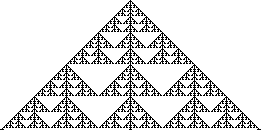
\includegraphics[width=7cm]{data/r150.png}\\
\hbox to 7cm{\hss pravidlo 86\hss}
\hfill
\hbox to 7cm{\hss pravidlo 150\hss}
}
\ods
\vbox{
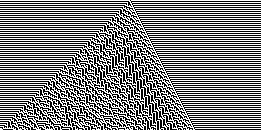
\includegraphics[width=7cm]{data/r89.png}
\hfill

\includegraphics[width=7cm]{data/r107.png}\\
\hbox to 7cm{\hss pravidlo 89\hss}
\hfill
\hbox to 7cm{\hss pravidlo 107\hss}
}

\ods
Rovnako dobre sa dá skúšať, čo sa stane, ak kolónia nezačína z jednej baktérie, ale z 
niekoľkých, ako sa správajú dve rastúce kolónie, ktoré do seba narazia, čo ak 
je pravidlo z väčšieho okolia a pod.
\fi

%%%%%%%%%%%%%%%%%%%%%%%%%%%%%%%%%%%%%%%%%%%%%%%%%%%%%%%%%%%%%%%%%%%%%%%%%%%%
\if\sectx1
\section{Funkcie}

Kapitolu~\ref{sec:CB obrazky} som začal tým, že som ti pripravil súbor, v ktorom
bol nový príkaz \prg!zapis_cb_png!. Teraz ti idem ukázať, ako si nové príkazy, ktorým
sa hovorí {\em funkcie}, môžeš vyrobiť aj ty. 
Možnosť vyrobiť si vlastné funkcie je veľmi dôležitá:
umožňuje ti rozdeliť si veľký program na malé časti, ktoré potom môžeš používať viackrát.

\ods
Najjednoduchšia funkcia vyzerá takto:

\vbox{
\begin{lstlisting}[] 
#include <iostream>
using namespace std;

int sedem() {
  return 7;
}

int main() {
  cout << sedem() << endl;
}
\end{lstlisting}
}

Všimni si, že sa veľmi podobá na zápis, ktorý používame na program. Nie je to náhoda.
Celý program je v skutočnosti len kopa funkcií, ibaže jedna z nich je špeciálna: tá, ktorá
sa volá \prg!main! sa začne vykonávať ako prvá. Každá funkcia je samostatný program,
ktorý má svoj vlastný svet.

\ods Funkcia má meno\footnote{Podobne
ako pri premenných, meno funkcie môže byť čokoľvek z veľkých a malých písmen, podčiarkovníkov
a čísel, ale nesmie začínať číslom.} a typ. V našom programe sme spravili funkciu, ktorá
sa volá {\tt sedem}. Typ \prg!int! pred jej menom hovorí, že táto funkcia predstavuje
výraz, ktorého výsledok je celé číslo.
Guľaté zátvorky za menom slúžia
na parametre. Zatiaľ žiadne nemáme, ale zátvorky aj tak treba písať. 
Potom nasleduje zložený príkaz, t.j. v kučeravých zátvorkách napísané príkazy. 

\ods Funkciu vieme v nejakej inej funkcii použiť ({\em zavolať}) tak, že napíšeme jej meno a parametre,
v našom prípade \prg!sedem()!. 
Pretože naša funkcia má typ \prg!int!, vieme, že každé jej zavolanie {\em vráti} celé číslo a
môžme ju použiť
vo výrazoch rovnako, ako by sme používali číslo. Môžeme napr. urobiť 
\prg!int x = 3 + sedem();! a pod. Kedykoľvek treba vyhodnotiť výraz, v ktorom
sa volá funkcia, všetko sa preruší a spustí sa tá funkcia. Príkaz
\prg!cout << sedem() << endl;! v našom programe hovorí \cmd{
  Začni vypisovať, mal by si vypísať číslo. Preruš robotu, spusti funkciu \prg!sedem()! 
  a počkaj, kým skončí.
Keď skončí, ako výsledok ti dá číslo. Pokračuj vo vypisovaní, vypíš  toto číslo a potom znak 
konca riadku.}

\ods Príkazy, ktoré sa vo funkcii vykonávajú sa volajú {\em telo} funkcie. Špeciálny 
príkaz \prg!return vyraz;! urobí to, že skončí funkciu a výsledok funkcie 
(tzv. {\em návratová hodnota}) bude hodnota výrazu \prg!vyraz!. Typ výrazu musí byť rovnaký
ako návratový typ funkcie, ktorý sme zadali pri jej definícii. Napr. naša funkcia
\prg!sedem()! vracia typ \prg!int!, preto výraz v príkaze \prg!return! musí mať hodnotu typu
\prg!int!. Funkcie ale môžu mať ako návratovú hodnotu ľubovoľný typ. Ak by som mal
funkciu \prg!bool zle() { return false; }!, môžem ju použiť všade, kde môžem mať výraz typu
\prg!bool!, napr. \prg!if (zle()) {}!.

\ods
Každá funkcia musí skončiť príkazom
\prg!return!\footnote{Slušné by bolo, aby sme aj na konci hlavného programu písali 
\prg!return 0;!, ale keďže už potom program skončí, tak to nevadí, keď to vynecháme.}.
Funkcia je samostatný svet, takže môže mať vlastné premenné. Tie sú úplne nezávislé
od iných funkcií (hovoríme im {\em lokálne premenné}). Čo urobí tento program?

\vbox{
\begin{lstlisting}[] 
#include <iostream>
using namespace std;

int pridaj() {
  int x;
  cin >> x;
  return x + 7;
}

int main() {
  int x = pridaj();
  cout << x + pridaj() << endl;
}
\end{lstlisting}
}

Hlavný program vyrobí premennú \prg!x!. Zavolá funkciu \prg!pridaj()! a jej
výsledok má uložiť do \prg!x!. Keď sa zavolá funkcia \prg!pridaj()!, vznikne 
nový svet, v ktorom sa vytvorí iná premenná \prg!x! a načíta sa do nej číslo zo vstupu.
Dajme tomu, že používateľ napíše 2.
Potom sa funkcia \prg!pridaj()! skončí, jej svet zanikne, a ostane len výsledok, číslo 9. 
Pracovať pokračuje hlavný program, do svojej premennej \prg!x! 
uloží výsledok volania funkcie, t.j. 9. Pokračuje príkazom \prg!cout <<!, 
na to potrebuje vyhodnotiť
výraz \prg!x + pridaj()!. V \prg!x! má 9, opäť preruší robotu a zavolá \prg!pridaj()!.
Zase vznikne nový svet s premennou \prg!x!, do ktorej sa prečíta hodnota. 
Dajme tomu, že teraz
je na vstupe 3. Funkcia skončí, jej svet zanikne a ostane číslo 10. Hlavný program
teraz dokončí rátanie výrazu \prg!9 + 10! a vypíše \prg!19!.

\ods
Doteraz sme nehovorili o parametroch. Parametre umožňujú používať tú istú funkciu na
rátanie rôznych vecí. Sú to premenné, ktoré sú lokálne premenné funkcie, ale
ich hodnota sa dá nastaviť zvonka pri volaní funkcie. Parametre a ich typy
sú uvedené v zátvorkách za menom funkcie, takže napr.

\vbox{
\begin{lstlisting}[] 
int scitaj(int x, int y) {
  int z = x + y;
  return z;
}
\end{lstlisting}
}

je funkcia, ktorá má dva parametre a oba sú celé čísla. Vo vnútri funkcie sa 
k nim dá správať ako k normálnym premenným. Majme hlavný program:

\vbox{
\begin{lstlisting}[] 
int main() {
  int x = 1;
  x = scitaj(x, scitaj(x, 3 * x));
  cout << x << endl;
}
\end{lstlisting}
}

Skús sa zamyslieť, čo vypíše. Máš to? Poďme to pozrieť detailne. Hlavný program
sa spustí, vyrobí si svoju premennú {\tt x} a dá do nej $1$. Potom ide
vyhodnocovať výraz, ktorého výsledok má uložiť do {\tt x} a zistí, že je to 
volanie funkcie.

\def\tw{2}
\def\th{3ex}
\def\r{1ex}
\def\vw{3.5ex}
\def\mimo{\color{black!50!white}}
\def\hi{\color{red!50!black}}
\def\dn{\color{blue!80!white}}
\def\fr#1{
  \draw[thick,draw=\clr,rounded corners=\r] (0,\th) rectangle (\tw,-\r);
  \filldraw[draw=none, fill=white] (0,0) rectangle (\w,-\h);
  \draw[thick,draw=\clr] (0,-\h) -- (0,0) -- (\w,0) -- (\w,-\h);
  \draw[thick,draw=none] (0,\th) rectangle node[color=\clr,anchor=center]{{\tt #1}} (\tw,0);
}
\def\var(#1,#2)#3#4#5{
  \draw (#1,#2) rectangle node[anchor=center]{#4} (#1+\vw,#2-\vw) 
  coordinate[pos=0.5] (#5);
  \node [anchor=east] at (#1,#2-0.5*\vw) {{\tt #3:}};
}

\def\conn[#1][#2](#3,#4){
    \draw[draw=orange, thick, ->, shorten >= 3ex, shorten <= 3ex] (#1) to[in=#3,out=#4] 
    node[midway, above, color=orange]{}(#2);
}
\ods
\begin{tikzpicture}
  \def\h{1.8}
  \def\w{6.2}
  \def\clr{green!55!black}
  \fr{main}
  \var(4ex,-1ex){x}{1}{mX}
  \node [anchor=south west] at (0,-10ex) {{\tt  
  {\mimo x = {\hi scitaj(}x, scitaj(x, 3 * x){\hi )}};}};
\end{tikzpicture}

\ods
Vyrobí sa teda nový svet funkcie {\tt scitaj} a hlavný program chce nastaviť
hodnoty parametrov. 
Prvý parameter nastaví podľa aktuálneho obsahu {\tt x}, 
ale pri druhom zistí, že je to výraz, v ktorom 
je opäť volanie funkcie.
 
\ods
\begin{tikzpicture}
  \def\h{1.8}
  \def\w{6.2}
  \def\clr{green!55!black}
  \fr{main}
  \var(4ex,-1ex){x}{1}{mX}
  \node [anchor=south west] at (0,-10ex) {{\tt  
  {\mimo x = {\dn scitaj(x, }{\hi scitaj(}x, 3 * x{\hi )}{\dn )}};}};

  \begin{scope}[shift={(8,-1)}]
  \def\h{1}
  \def\w{4}
  \def\clr{blue!55!black}
  \fr{scitaj}
  \var(4ex,-1ex){x}{1}{vX}  
  \var(15ex,-1ex){y}{}{vY}  
  \draw[draw=\clr](0,-5ex) -- (\w,-5ex); 
  \conn[mX][vX](150,10);
  \end{scope}
\end{tikzpicture}

\ods Vytvorí sa teda ďalší, nezávislý, svet funkcie {\tt scitaj}, nastavia sa mu hodnoty
parametrov a vyráta sa výsledok, ktorý sa potom vráti tomu, kto funkciu zavolal.

\ods
\begin{tikzpicture}
  \def\h{1.8}
  \def\w{6.2}
  \def\clr{green!55!black}
  \fr{main}
  \var(4ex,-1ex){x}{1}{mX}
  \node [anchor=south west] at (0,-10ex) {{\tt  
  {\mimo x = {\dn scitaj(x, }{\hi scitaj(}x, 3 * x{\hi )}{\dn )}};}};

  \begin{scope}[shift={(9,1)}]
  \def\h{1}
  \def\w{4}
  \def\clr{blue!55!black}
  \fr{scitaj}
  \var(4ex,-1ex){x}{1}{vX}  
  \var(15ex,-1ex){y}{}{vY}  
  \draw[draw=\clr](0,-5ex) -- (\w,-5ex); 
  \end{scope}
  
  \begin{scope}[shift={(7.5,-1.5)}]
  \def\h{2.6}
  \def\w{4}
  \def\clr{orange!55!black}
  \fr{scitaj}
  \var(4ex,-1ex){x}{1}{vvX}  
  \var(15ex,-1ex){y}{3}{vvY}  
  \draw[draw=\clr](0,-5ex) -- (\w,-5ex); 
  \conn[mX][vvX](150,10);
  \conn[mX][vvY](150,10);
  \var(4ex,-6ex){z}{4}{vvZ}  
    \node [anchor=south west] at (0,-13ex) {{\tt ... }};
    \node [anchor=south west] at (0,-16ex) {{\tt return z;}};
  \draw[draw=\clr](0,-\h) -- (\w,-\h); 
  \end{scope}
\end{tikzpicture}

\ods Teraz druhý svet zanikne, ostane z neho iba výsledok $4$, a tým sa nastaví parameter
v prvom svete:

\ods
\begin{tikzpicture}
  \def\h{1.8}
  \def\w{6.2}
  \def\clr{green!55!black}
  \fr{main}
  \var(4ex,-1ex){x}{1}{mX}
  \node [anchor=south west] at (0,-10ex) {{\tt  
  {\mimo x = {\dn scitaj(x, }{\color{white} scitaj(x, 3 * x )}{\dn )}};}};
  \node[anchor=south west] (vys) at (24ex,-10ex) {\color{orange} 4};

  \begin{scope}[shift={(8,-0.5)}]
  \def\h{2.6}
  \def\w{4}
  \def\clr{blue!55!black}
  \fr{scitaj}
  \var(4ex,-1ex){x}{1}{vX}  
  \var(15ex,-1ex){y}{4}{vY}  
  \draw[draw=\clr](0,-5ex) -- (\w,-5ex); 
  \var(4ex,-6ex){z}{5}{vZ}  
    \node [anchor=south west] at (0,-13ex) {{\tt ... }};
    \node [anchor=south west] at (0,-16ex) {{\tt return z;}};
  \draw[draw=\clr](0,-\h) -- (\w,-\h); 
  \end{scope}
 
  \conn[vys][vY](150,10);
\end{tikzpicture}

\ods
Napokon zanikne aj prvý svet, ostane hodnota 5 a tá sa zapíše do premennej {\tt x}
v hlavnom programe. Takže si to zhrňme: funkcia je samostatný program, ktorý má 
výstupnú hodnotu\footnote{Tu len pripomeniem: úplne na začiatku sme hovorili,
že najjednoduchší príkaz {\tt 3*(2+5);} len vyráta hodnotu $21$ a výsledok zahodí. 
To je, samozrejme, zbytočné, ale niekedy môžeš chcieť zahodiť hodnotu funkcie. Napríklad
volanie \prg!pridaj();! z predchádzajúceho odstavca načíta číslo zo vstupu a 
ignoruje ho.}.
Dá sa použiť vo výrazoch. Pri volaní funkcie sa vytvorí
nový nezávislý svet, nastavia sa hodnoty parametrov\footnote{%
Zatiaľ vieme ako parametre funkciám posielať premenné, ale nie polia. 
Polia sa tiež dajú ako parametre použiť, ale o tom až neskôr.
} a vypočíta sa výstupná hodnota.

\begin{uloha}
  Napíš funkciu {\tt max} s tromi parametrami, ktorá vráti najväčší z nich.
\end{uloha}

\ods
Doposiaľ sme mali každú premennú vyrobenú v nejakej funkcii (či už {\tt main} alebo 
v nejakej inej). Dajú sa však vyrobiť aj premenné, ktoré žiadnej funkcii nepatria
a sú viditeľné z každého sveta: hovorí sa im {\em globálne premenné}. Najľahšie
sa to ukáže na píklade:

\vbox{
\begin{lstlisting}[] 
#include <iostream>
using namespace std;

int a;

void pridaj(int kolko) { a = a + kolko; }

int main() {
  int i;
  a = 0;
  for (i = 0; i < 10; i++) pridaj(i);
  cout << a << endl;
}
\end{lstlisting}
}

\ods
Tu sme vyrobili globálnu premennú {\tt a}. Keďže je vyrobená skôr, ako
definujeme funkciu {\tt pridaj}, telo funkcie môže k premennej {\tt a} pristupovať.
Tu som použil ako návratový typ nový typ: \prg!void!. Je to prázdny typ, ktorým hovoríme,
že funkciu chcem vždy použiť iba v situácii, keď výslednú hodnotu zahodím. Takéto funkcie
nemusia končiť príkazom \prg!return!. Po spustení program vypíše $0+1+2+\cdots+9=45$.

\ods Poznámka o viditeľnosti: rovnako ako pri funkciách sa samostatný svet
vyrába aj pri zložených príkazoch. To znamená, že svety môžu zapadať jeden do druhého:
svet globálnych premenných, v ňom svet funckie, v ňom svet zloženého príkazu,\ldots.
Vždy, keď program pristupuje k nejakej premennej,
vyberie sa premenná s požadovaným menom z najbližšieho sveta, v ktorom taká je. 
Napr. program

\vbox{
\begin{lstlisting}[] 
#include <iostream>
using namespace std;

int x = 5;

void p() { cout << x; }

int main() {
  int x = 7;
  int a = 9;
  cout << x;
  p();
  {
    int x = 6;
    cout << x << a;
    p();
  }
  cout << x << endl;
}
\end{lstlisting}
}

vypíše {\tt 756957}: funkcia {\tt p} vo svojom svete nemá premennú {\tt x}, preto sa použije
globálna {\tt x}. Funkcia {\tt main} má svoju vlastnú {\tt x}, preto sa použije tá.
Zložený príkaz má svoj vlastný svet, v ktorom má svoju vlastnú {\tt x}, ale {\tt a}
sa použije zo sveta {\tt main}.

\ods
Globálne premenné môžu byť rovnako dobre aj  polia. Tu je ale problém, akú veľkosť má
pole mať. Pretože ho vyrábam skôr, ako sa spustí hlavný program, nemôžem čakať, kým
zo vstupu dostanem veľkosť poľa. Najjednoduchší spôsob je povedať si dopredu ohraničenie
na veľkosť poľa, vyrobiť dostatočne veľké pole a potom z neho použiť len potrebný kus.
Toto nie je ideálny prístup (okrem iného mrhá pamäťou), ale nateraz nám postačí.
Napr. tento program:

\vbox{
\begin{lstlisting}[] 
#include <iostream>
using namespace std;

int a[1000];

int main() {
  int n = -1;
  do {
    n++;
    cin >> a[n];
  } while (a[n] > 0);
}
\end{lstlisting}
}

číta do poľa {\tt a} vstupné kladné čísla a skončí, keď sa prvýkrát prečíta niečo 
$\le 0$. V premennej {\tt n} (ktorá je lokálna funkcii {\tt main}) je uložená ''skutočná''
dĺžka poľa. Ak by bolo na vstupe viac ako 1000 čísel, stanú sa hrozné veci.

\begin{uloha}
  \label{uloha:sort2}
  Napíš funkciu s parametromm \prg!int n!, ktorá v globálnom poli {\tt a} 
  (o ktorom predpokladáme, že obsahuje kladné čísla) nájde najväčší
  prvok spomedzi prvých {\tt n}, prepíše ho v poli na {\tt -1} a vráti jeho hodnotu
  (ešte predtým, ako ho prepísala). Potom s pomocou nej
  napíš program, ktorý do poľa prečíta kladné
  čísla zo vstupu a vypíše ich v utriedenom poradí.
\end{uloha}

Na ľahšiu prácu s globálnymi premennými je v súbore {\tt obrazok.h}
definovaná funkcia {\tt zapis\_cb\_png\_vyrez}, ktorá má dodatočné
štyri parametre. Tie hovoria, ktoré riadky a ktoré stĺpce sa majú do obrázka zapísať.
Program

\vbox{
\begin{lstlisting}[] 
#include <iostream>
#include "obrazok.h"
using namespace std;

const int N = 2000;
int a[N][N];

int main() {
  // tuto niečo nakresli
  zapis_cb_png_vyrez(N, N, a, "vystup.png", 50, 80, 300, 200);
}
\end{lstlisting}
}

vypíše do súboru {\tt vystup.png} výrez z poľa {\tt a}  tvorený riadkami
$50$ až $299$ a stĺpcami $80$ až $199$. Pretože {\tt a} je teraz vyrobené ako globálna
premenná, jeho rozmery musia byť známe už v čase kompilácie. Na to je špeciálny
modifikátor \prg!const!, ktorý sme použili pri vytváraní premennej {\tt N} a ktorý
hovorí, že {\tt N} sa v programe nebude meniť (môžeš si vyskúšať, že to nejde).

\begin{uloha}
  Napíš funkciu \prg!void stvorec(int r, int s, int d)!, ktorá v globálnom poli
  vyplní jednotkami štovrec $d\times d$ začínajúci na riadku $r$ a stĺpci $s$.
  S jej pomocou napíš program, ktorý načíta tri čísla $a, b, c$ také, že
  $a+b+c<100$ a vyrobí obrázok rozmerov $100\times 100$, v ktorom budú tri štvorce
  rozmerov $a\times a$, $b\times b$ a $c\times c$ položené jeden na druhom 
  v strede obrázka. Napr. pre vstup $40, 30, 20$ bude obrázok vyzerať takto:

\ods
 {
\setlength{\fboxsep}{0pt}
\centerline{\fbox{
\includegraphics[width=4cm]{data/tristvorce.png}}}
  }
\end{uloha}
\fi

%%%%%%%%%%%%%%%%%%%%%%%%%%%%%%%%%%%%%%%%%%%%%%%%%%%%%%%%%%%%%%%%%%%%%%%%%%%%
\if\sectxi1
\section{Rekurzia}

Volanie funkcie pri vyhodnocovaní výrazu, ako sme ho opísali v minulej kapitole,
nemusí byť len z hlavného programu, ale z hocijakej funkcie, tento program
vypíše 16:

\vbox{
\begin{lstlisting}[] 
#include <iostream>
using namespace std;

int a(int x) { return x + 1; }

int b(int x) { return a(x) * a(x); }

int main() { cout << b(3) << endl; }
\end{lstlisting}
}

Jediná vec, ktorú treba dodržať je, podobne ako pri premenných, že každé použitie
(volanie) musí byť až vtedy, keď funkcia bola v programe vyrobená. Keby si
napr. v predchádzajúcom programe prehodil riadky s definíciou funkcií {\tt a} a {\tt b},
nefungoval by. 

\ods Špeciálne zaujímavá je situácia, keď funkcia vo svojom tele volá sama seba. Takéto
volanie je možné a hovorí sa mu {\em rekurzia}. Na prvý pohľad to možno vyzerá divne, ale
nie je to. Treba len, podobne ako pri cykle, zabezpečiť, aby sa volanie nezacyklilo
ako táto funkcia:

\vbox{
\begin{lstlisting}[] 
int a(int x) { return 1 + a(x + 1); }
\end{lstlisting}
}

\ods
Čo sa začne diať, ak zavoláš \prg!a(0)!? Najprv sa spraví nový svet funkcie \prg!a!,
v ktorom sa {\tt x} nastaví na 0 a začne sa vykonávať telo funkcie. V ňom
sa spraví nový nezávislý svet funkcie {\tt a}, v ktorom sa  {\tt x} nastaví na 1
a začne sa vykonávať telo funkcie. V ňom
sa spraví nový nezávislý svet funkcie {\tt a}, v ktorom sa  {\tt x} nastaví na 2
a začne sa vykonávať telo funkcie. V ňom
sa spraví nový nezávislý svet funkcie {\tt a}, v ktorom sa \ldots


\ods
Keď ale funkcii naprogramuješ správne ''dno'', niektoré rekurzívne formulácie
sú veľmi prirodzené. Zober si napríklad hľadanie najväčšieho spoločného deliteľa.
Euklides vedel, že ak máme dve čísla $a$ a $b$ také, že $a>b$, 
a obidve sú deliteľné číslom $k$,
to znamená že $a=xk$ a $b=yk$ pre nejaké $x$ a $y$. Potom $a-b=xk-yk=(x-y)k$,
a teda aj $x-y$ je deliteľné číslom $k$. Preto každý spoločný deliteľ $a$ a $b$
je zároveň spoločným deliteľom $a-b$ a $b$. Najväčšieho spoločného deliteľa
preto vieme nájsť takto:

\vbox{
\begin{lstlisting}[] 
int NSD(int a, int b) {
  if (a == b) return a;
  if (a == 1 || b == 1) return 1;
  if (a > b) return NSD(a - b, b);
  return NSD(b - a, a);
}
\end{lstlisting}
}

Keď zavoláme napr \prg!NSD(4,6)!, toto volanie následne zavolá \prg!NSD(2,4)!,
toto zase \prg!NSD(2,2)! a toto volanie už ďalší svet {\tt NSD} nevytvorí,
ale vráti 2. Potom už reťazovo všetky ostatné volania dobehnú a vrátia 2.
Ako sa presvedčíme, že sa táto funkcia nikdy nezacyklí? Všimni si, že keď
funkciu zavoláme s hocijakými $a>0$, $b>0$, každé ďalšie volanie zmenší
súčet $a+b$. Zároveň ani $a$, ani $b$ neklesne na nulu (to by museli byť 
v predchádzajúcom volaní rovnaké, ale vtedy by sa už ďalšie volanie nevyrobilo).
Keďže súčet nemôže klesať donekonečna, vidíme, že funkcia sa nikdy nezacyklí.

\ods S rekurziu sa často stretneš pri definícii rôznych výrazov. Napríklad takto:
\begin{uloha}
  \label{uloha:vyrazy}
  Zjednodušený výraz je buď jednociferné číslo, alebo má tvar 
  {\tt ($\clubsuit$+$\heartsuit$)}, kde $\clubsuit$ a $\heartsuit$ sú zjednodušené
  výrazy. Zjednodušený výraz končí znakom {\tt\$}. 
  Napíš program, ktorý prečíta zo vstupu zjednodušený výraz a vyráta jeho
  hodnotu.
\end{uloha}

Zo zadania vidíme, že zjednodušené výrazy sú napr. {\tt 4\$} alebo
alebo {\tt (2+((3*2)+(1+(6*3))))\$}, ale nie {\tt 12\$} (nie je jednociferné), ani 
{\tt 5+1\$} (nie je v zátvorkách), ani {\tt (3+8+1)\$}. 
Na čítanie vstupu použijeme premennú typu \prg!char c;! (pozri kapitolu \ref{sect:cisla}).
Príkaz \prg!cin >> c;! prečíta jeden znak zo vstupu\footnote{%
Ako sme v kapitole \ref{sect:cisla} hovorili, pri načítavaní sa preskakujú whitespace
znaky.  Toto správanie sa dá prepnúť,
ak z \prg!cin! načítaš špeciálnu hodnotu \prg!noskipws!, t.j. \prg!cin >> noskipws;!
spôsobí, že sa budú načítavať všetky znaky vrátane medzier.
}. Ak je tento znak číslica, t.j.
\prg!c>='0' && c<='9'!, tak hodnota výrazu je číslo, ktoré táto číslica reprezentuje,
t.j. \prg!c-'0';! (tu využívame, že v ASCII tabuľke idú znaky číslic za sebou).
Ak prvý znak nebola číslica, musela to byť otváracia zátvorka. Hodnotu výrazu potom
získame tak, že rekurzívne vyhodnotíme prvý výraz, prečítame znak operácie, rekurzívne
vyhodnotíme druhý výraz a vrátime výsledok (predtým ale nezabudneme prečítať
zatváraciu zátvorku). Výsledok by mohol vyzerať takto:

\vbox{
\begin{lstlisting}[] 
int vyraz() {
  char c;
  cin >> c;
  if (c >= '0' && c <= '9') return c - '0';
  int v1 = vyraz(); // rekurzivne volanie 
  cin >> c;         // operator
  int v2 = vyraz(); // druhe rekurzivne volanie 
  int vysledok;
  if (c == '+')
    vysledok = v1 + v2;
  else
    vysledok = v1 * v2;
  cin >> c;         // zatvaracia zatvorka
  return vysledok;
}
\end{lstlisting}
}

\ods
Keby si chcel mať viacciferné čísla, uvedom si, že napr. hodnota čísla \prg!'4567'! je
desaťkrát hodnota čísla \prg!'456'! plus hodnota cifry \prg!'7'!.

\begin{uloha}
  Uprav predchádzajúce riešenie tak, aby pracovalo s viaccifernými číslami.
\end{uloha}

\begin{uloha}
  Napíš program, ktorý načíta zo vstupu jedno prirodzené číslo a vypíše ho otočené.
  Má to ale háčik: v celom programe môžeš použiť iba jedinú premennú (tú, do 
  ktorej načítaš vstup).
\end{uloha}

Niekedy je dobé mať globálnu premennú (napr. pole), do ktorého rekurzívna procedúra
postupne generuje všetky možnosti: skúsi prvú možnosť, rekurzívne doplní zvyšok, skúsi
druhú možnosť, atď.


\begin{uloha}
Napíš program, ktorý prečíta číslo $n$ a vypíše všetky možné usporiadania
  čísel $1,2,\ldots,n$. Napr. pre $n=3$ vypíše (v nejakom poradí):
  \begin{verbatim}
1 2 3
1 3 2
2 1 3
2 3 1
3 2 1
3 1 2
\end{verbatim}
\end{uloha}

\begin{uloha}
Napíš program, ktorý prečíta čísla $n$, $m$, $k$
  a vypíše všetky postupnosti dĺžky $n$ zložené z čísel {\tt 0,1,2}, ktoré obsahujú
  $m$ jednotiek, $k$ dvojok a ostatné sú nuly. Napr. pre vstup {\tt 4 2 1} vypíše
  $12$ možností:

  \ods
\begin{minipage}[t]{0.3\textwidth}
\begin{verbatim}
0 1 1 2 
0 1 2 1 
0 2 1 1 
1 0 1 2 
\end{verbatim}
\end{minipage}
\hfill
\begin{minipage}[t]{0.3\textwidth}
\begin{verbatim}
1 0 2 1 
1 1 0 2 
1 1 2 0 
1 2 0 1 
\end{verbatim}
\end{minipage}
\hfill
\begin{minipage}[t]{0.3\textwidth}
\begin{verbatim}
1 2 1 0 
2 0 1 1 
2 1 0 1 
2 1 1 0
\end{verbatim}
\end{minipage}

\end{uloha}

\begin{uloha}
  \label{uloha:fill}
  Na vstupe sú čísla $n$, $m$ a dvojrozmerné pole núl a jednotiek s $n$ riadkami
  a $m$ stĺpcami. Napokon sú tam dve čísla $r$, $s$.
  Napíš program, ktorý vyplní jednotkami uzavretú oblasť núl ohraničenú jednotkami,
  ktorá obsahuje políčko na riadku $r$ a stĺpci $s$.
  Konkrétne treba urobiť toto: prefarbiť políčko na riadku $r$ a stĺpci $s$ na 1,
  pozrieť sa na štyroch susedov (hore, dole, vľavo a vpravo) a pre každého z nich,
  ktorý má hodnotu 0, urobiť to isté (t.j. prefarbiť ho na 1, pozrieť sa na štyroch 
  susedov, \ldots)


  \ods
\bp
\inp
\begin{verbatim}
8 11
0 0 1 1 1 1 0 0 0 0 0
0 1 0 0 0 0 1 0 0 1 0
0 1 0 0 0 0 1 0 1 0 1
0 0 1 0 0 0 1 0 1 0 1
0 0 1 0 0 1 0 0 1 0 1
0 0 1 0 1 0 1 1 1 0 1 
0 0 1 0 0 0 0 0 0 0 1 
0 0 0 1 1 1 1 1 1 1 0 
2 4
\end{verbatim}
\ep
\hfill
\bp
\outp
\begin{verbatim}
0 0 1 1 1 1 0 0 0 0 0
0 1 1 1 1 1 1 0 0 1 0
0 1 1 1 1 1 1 0 1 1 1
0 0 1 1 1 1 1 0 1 1 1
0 0 1 1 1 1 0 0 1 1 1
0 0 1 1 1 1 1 1 1 1 1 
0 0 1 1 1 1 1 1 1 1 1 
0 0 0 1 1 1 1 1 1 1 0 
\end{verbatim}
\ep

\end{uloha}

\begin{uloha}
  \def\sierp#1{
    \def\tre{0.333333333}
    \if#10
    \filldraw(0,0) rectangle (1,1);
    \else
    \foreach \x in {0,...,2}
    \foreach \y in {0,...,2} {
      \pgfmathparse{\x==1 && \y==1?int(1):int(0)}
      \ifnum\pgfmathresult=0{
        \begin{scope}[shift={(\tre*\x,\tre*\y)}, scale=\tre]
          \pgfmathtruncatemacro{\n}{#1-1}
          \sierp{\n}
        \end{scope}
      }
      \fi
    }
    \fi 
  }

  Sierpińského koberec je vzor, ktorý je popísaný rekurzívne. Koberec úrovne nula
  je čierny štvorec. Koberec úrovne $n$ dostaneme tak, že zoberieme štvorec, rozdelíme
  ho na mriežku $3\times3$, stredný štvorec vyrežeme, a osem zvyšných štvorcov nahradíme
  kópiami koberca úrovne $n-1$. Prvých päť kobercov vyzerá takto:

  \ods
  \begin{tikzpicture}[scale=2.8]
    \foreach\i in {0,...,\if\longSierp14\else1\fi} {
    \begin{scope}[shift={(\i*1.1,0)}]
      \sierp{\i}
    \end{scope}}
  \end{tikzpicture}

  \ods
  Napíš program, ktorý zo vstupu prečíta $n$ a vyrobí obrázok rozmerov
  $3^n\times3^n$ (t.j. úroveň 0 má stranu dĺžky $1$, úroveň $1$ stranu $3$,
  a úroveň $n$ stranu $3^n=\overbrace{3\cdot3\cdots3}^n$), v ktorom bude koberec úrovne $n$.
\end{uloha}

\fi

%%%%%%%%%%%%%%%%%%%%%%%%%%%%%%%%%%%%%%%%%%%%%%%%%%%%%%%%%%%%%%%%%%%%%%%%%%%%
\if\sectxii1
\section{Zložitosť}
\label{sect:zlozitost}

Keď máme niečo naprogramovať, väčšinou je viac možností, ako to urobiť. A nie všetky sú 
rovnako dobré. Fibonacciho čísla z úlohy~\ref{uloha:Fibonacci} môžem naprogramovať
dvoma spôsobmi takto:

\ods
\bp
\begin{lstlisting}[] 
long int Fib1(int n) {
  if (n < 3) return n - 1;
  long int a = 0, b = 1, c;
  int i;
  for (i = 2; i < n; i++) {
    c = a + b;
    a = b;
    b = c;
  }
  return c;
}
\end{lstlisting}
\ep
\hfil
\bp
\begin{lstlisting}[] 
long int Fib2(int n) {
  if (n < 3) return n - 1;
  return Fib2(n - 1) + Fib2(n - 2);
}
\end{lstlisting}
\ep

\ods
Rekurzívna verzia vpravo je kratšia a lepšie pochopiteľná, lebo z nej priamo vidíme
posup \cmd{$n$-té číslo vyrátaš tak, že sčítaš dve predchádzajúce}.
Má to ale háčik. Začal som si merať čas, koľko trvá, kým sa vyráta $n$-té číslo. 
Funkcia \prg!Fib1! všetky čísla po $90$ (cca toľko sa zmestí do \prg!long int!) vyrátala
pod jednu milisekundu. Pri funkcii \prg!Fib2! som sa dostal po $54$-té číslo. Tam to trvalo
cca 518 sekúnd a potom ma to prestalo baviť. Tu vidíš graf, ako závisel čas behu od veľkosti
$n$. Čísla {\tt Fib2(90)} by som sa nedočkal ani do konca vesmíru.

\ods
\begin{tikzpicture}
\begin{axis}[
  width=\textwidth, 
  height=10cm,
  xlabel=$n$,
  ylabel=čas (s),
  legend cell align={left},
  legend pos = north west
]
  \addplot+[blue!80!white, 
  line join=round, mark size=0.5pt] table [y=f, x=n]{data/fibcas.dat};
  \addlegendentry{koľko sekúnd trvá vyrátať {\tt Fib2(n)}}
\end{axis}
\end{tikzpicture}

\ods
Problém tu bol v tom, že rekurzívna verzia ráta veľa vecí zbytočne: keď chce vyrátať
{\tt Fib2(10)}, najprv ráta {\tt Fib2(9)}. Pri rátaní {\tt Fib2(9)}, vyráta 
{\tt Fib2(8)=13}
a {\tt Fib2(7)=8}, takže vráti hodnotu {\tt Fib2(9)=21}. Pokračuje sa v rátaní
{\tt Fib2(10)}: {\tt Fib2(9)} už je vyrátané, ide sa 
 rátať {\tt Fib2(8)}. To sa už síce raz rátalo, ale výsledok
zanikol spolu so svetom predchádzajúceho rekurzívneho volania, takže sa bude rátať
znova. Takto sa nabaľuje veľa 
zbytočnej práce a už aj pre relatívne malé $n$ to začne byť celkom dosť problém.

\ods
Keď máme dva programy, ako môžeme povedať, ktorý z nich je rýchlejší?
Keby som ti povedal, že vyrátať 37. Fibonacciho číslo mi tvalo 140 ms, nič ti to nepovie,
lebo to závisí od toho, aký mám rýchly počítač. Hlavný problém s funkciou {\tt Fib2} nebol 
v konkrétnych časoch, ale v tom, že sa príliš rýchlo zväčšovali. Chceme teda vymyslieť 
spôsob, ako povedať, ako rýchlo rastie čas programu v závislosti od veľkosti vstupu.
Ukážeme si to na príklade. Povedzme, že už máme načítané pole {\tt a},
v ktorom je $n$ čísel, každé
z nich z rozsahu $0,\ldots,999$. 
Chcem ho preusporiadať tak, aby bolo v poradí od najväčšieho čísla po najmenšie.
Podobný problém si už riešil v úlohách~\ref{uloha:sort1} a \ref{uloha:sort2}, 
teraz skúsme trochu iný prístup, vlastne dva.

\ods
Prvý algoritmus je tzv. {\em Insertion Sort}. Idea je takáto: budeme sa snažiť
prehadzovať prvky v poli tak, aby nakoniec polo utriedené. Algoritmus bude pracovať v
kolách. Na začiatku $i$-teho kola chceme, aby platilo, že prvých $i$ pozícií je
utriedených. Na začiatku prvého kola to platí -- prvý jeden prvok je utriedený vždy.
Ak sa nám podarí, aby to platilo aj po $n$ kolách, budeme mať utriedených
prvých $n$ pozícií, t.j. celé pole. Predpokladajme teraz, že sme na začiaku $i$-teho kola.
Skontrolujeme, či je prvok {\tt a[i]} je menší, ako {\tt a[i-1]}. 
Ak áno, môžeme toto kolo skončiť,
lebo prvých $i+1$ prvkov je utriedených. Ak nie, vymeníme prvky {\tt a[i]} a 
{\tt a[i-1]}
a skontrolujeme, či je {\tt a[i-1]} menší ako {\tt a[i-2]}. Takto pokračujeme ďalej, kým
nedostaneme prvok {\tt a[i]} na správne miesto:

\ods
\begin{tikzpicture}[xscale=0.132,yscale=0.135]
  \def\bar(#1,#2)#3{
    \filldraw[draw=black,fill=#3](#1,0) rectangle (#1+1,#2);
  }
  \def\prf{orange!60!white}
  \def\rst{rgb:green,5;yellow,4;blue,2;black,3}
  \def\act{rgb:blue,5;green,3;white,4}
  \def\base{
    \foreach \x[count=\i] in {20,19,17,15,14,13} {
      \bar(\i,\x){\prf}
    }
    \foreach \x[count=\i] in {12,4,3,18,7} {
      \bar(\i+11,\x){\rst}
    }
    \draw [<-, shorten <= 4] (11.5,0) -- (11.5,-4) node [anchor=north]{$i$};
  }
  \def\dj#1{  
  \draw [<-, shorten <= 5] (#1+.5,11) -- (#1+.5,19) node [anchor=south]{$j$};
  }
  \def\sh{23}

  \begin{scope}[shift={(0,0)}]
    \base
    \foreach \x[count=\i] in {10,9,8,5} {
      \bar(\i+6,\x){\prf}
    }
    \bar(11,11.5){\act}
    \dj{11}
  \end{scope}

  \begin{scope}[shift={(\sh,0)}]
    \base
    \foreach \x[count=\i] in {10,9,8} {
      \bar(\i+6,\x){\prf}
    }
    \bar(10,11.5){\act}
    \bar(11,5){\prf}
    \dj{10}
  \end{scope}

  \begin{scope}[shift={(2*\sh,0)}]
    \base
    \foreach \x[count=\i] in {10,9} {
      \bar(\i+6,\x){\prf}
    }
    \bar(9,11.5){\act}
    \bar(10,8){\prf}
    \bar(11,5){\prf}
    \dj{9}
  \end{scope}

  \begin{scope}[shift={(3*\sh,0)}]
    \base
    \bar(7,10){\prf}
    \bar(8,11.5){\act}
    \bar(9,9){\prf}
    \bar(10,8){\prf}
    \bar(11,5){\prf}
    \dj{8}
  \end{scope}

  \begin{scope}[shift={(4*\sh,0)}]
    \base
    \bar(7,11.5){\act}
    \bar(8,10){\prf}
    \bar(9,9){\prf}
    \bar(10,8){\prf}
    \bar(11,5){\prf}
    \dj{7}
  \end{scope}
\end{tikzpicture}

\ods
Celá funkcia bude vyzerať takto\footnote{%
  premysli si, čo by sa stalo, keby som vo funkcii {\tt vymen} napísal iba
  \prg!a[i]=a[j]; a[j]=a[i];!
}:

\ods
\vbox{
\begin{lstlisting}[] 
void vymen(int i, int j) {
  int x;
  x = a[i];
  a[i] = a[j];
  a[j] = x;
}

void InsertSort(int n) {
  int i, j;
  for (i = 1; i < n; i++)
    for (j = i; j > 0 && a[j - 1] < a[j]; j--) 
      vymen(j - 1, j);
}
\end{lstlisting}
}

\ods
Druhý algoritmus, tzv. {\em CountSort} 
vychádza z toho, že vieme, že vstupné čísla sú z malého rozsahu
(od 0 do 999). Vyrobíme si pomocné pole \prg!pocty[1000]!, v ktorom si budeme
pamätať počty jednotlivých prvkov (\prg!pocty[i]==j! namená, že sa v poli vyskytuje
{\tt j}-krát hodnota {\tt i}). Takže raz prejdeme vstupným poľom a zistíme počty
a potom len zapíšeme správny počet hodnôt takto:

\ods
\vbox{
\begin{lstlisting}[] 
void CountSort(int n) {
  int pocty[1000];
  int i, c;

  for (i = 0; i < 1000; i++) pocty[i] = 0;
  for (i = 0; i < n; i++) pocty[a[i]]++;
  i = 0;
  for (c = 999; c>=0 ; c--)
    while (pocty[c] > 0) {
      a[i] = c;
      i++;
      pocty[c]--;
    }
}
\end{lstlisting}
}

\ods
Teraz som spravil to, že som oba algoritmy veľakrát spustil na rôznych poliach
a meral im čas. Výsledky sú v nasledovných grafoch\footnote{Vyzerajú síce podobne, 
ale všimni si, že obrázok vľavo je v sekundách a vpravo v mikrosekundách. CounSort
bol na dlhých poliach výrazne rýchlejší.}

\if\longCharts1
\ods
\begin{tikzpicture}
\begin{axis}[
  title={InseretSort},
  width=0.5*\textwidth, 
  height=10cm,
  xlabel=$n$,
  ylabel=čas (s),
  scaled x ticks=false,
  scaled y ticks=false,
  domain=0:20000,
  xmin=0,
  xmax=20000,
  /pgf/number format/.cd,
        1000 sep={}
]
  \addplot+[only marks, mark size=0.4pt, mark options={
    draw=orange!80!white,
    fill=red!80!orange
  }
  ] 
  table [y expr=\thisrow{t}/1000000, x=n, ]{data/is.dat};
  \addplot[no markers,red!50!white]{0.0000000027*x*x+0.01};
\end{axis}
\end{tikzpicture}
\begin{tikzpicture}
\begin{axis}[
  title={CountSort},
  width=0.5*\textwidth, 
  height=10cm,
  xlabel=$n$,
  ylabel=čas ($\mu$s),
  scaled x ticks=false,
  scaled y ticks=false,
  domain=0:20000,
  xmin=0,
  xmax=20000,
  /pgf/number format/.cd,
        1000 sep={}
]
  \addplot+[only marks, mark size=0.4pt, mark options={
    draw=cyan!80!white,
    fill=blue!80!cyan
  }
  ] 
  table [y=t, x=n ]{data/cs.dat};
  \addplot[no markers,blue!50!white]{0.015*x+25};
\end{axis}
\end{tikzpicture}
\fi

\ods
Z grafov vidno, že obom algoritmom dlhšie polia trvajú dlhšie, ale aj na rovnako dlhých
poliach môžu bežať rôzne dlho (podľa toho, aké konkrétne čísla v tom poli sú).
Ničmenej všetky body na ľavom obrázku sa dajú schovať pod parabolu\footnote{%
  graf funkcie $y=ax^2+b$ pre nejaké čísla $a$, $b$} a všetky body vpravo 
  pod priamku. Preto hovoríme, že InsertSort má {\em kvadratickú zložitosť}, kým
CountSort má {\em lineárnu}.

\ods
Je algoritmus s lineárnou zložitosťou vždy lepší, ako ten s kvadratickou?
Predpokladajme, že máme lineárny algoritmus ${\cal A}$, ktorého čas na vstupe veľkosti
$n$ je najviac $42n+200$. Majme hocijaký kvadratický algoritmus ${\cal B}$,
ktorého čas na vstupe veľkosti $n$ je $an^2+b$ pre nejaké čísla $a$, $b$. 
Pre malé hodnoty $n$ môže byť algoritmus ${\cal B}$ rýchlejší. Ale existuje
$n$, kedy $24n+200=an^2+b$, a od tohto $n$ ďalej už bude rýchlejší algoritmus 
${\cal A}$. 

\ods
\centerline{
\begin{tikzpicture}
\begin{axis}[
  width=0.7*\textwidth, 
  height=7cm,
  xlabel=$n$,
  %scaled x ticks=false,
  scaled y ticks=false,
  domain=0:20000,
  xmin=0,
  xmax=20000,
  /pgf/number format/.cd,
        1000 sep={},
  legend cell align={left},
  legend pos = south east
]
  \addplot[no markers,red!50!white]{42*x+200};
  \addlegendentry{$42x+200$}
  \addplot[domain=0:3200,no markers,teal!40!white]{0.1*x*x};
  \addlegendentry{$0.1x^2$}
  \addplot[domain=0:10000,no markers,teal!60!white]{0.01*x*x};
  \addlegendentry{$0.01x^2$}
  \addplot[domain=0:14000,no markers,teal!80!white]{0.005*x*x};
  \addlegendentry{$0.005x^2$}
  \addplot[domain=0:19500,no markers,teal]{0.0025*x*x};
  \addlegendentry{$0.0025x^2$}
\end{axis}
\end{tikzpicture}}

\ods
Inými slovami, pre každý kvadratický algoritmus platí, že pre dosť veľké vstupy je
${\cal A}$ rýchlejší. Podobne vieme hovoriť o kubických algoritmoch, algoritmoch štvrtého 
stupňa atď. A ako by dopadol algoritmus {\tt Fib2}? Jeho zložitosť je až $2^n$: rastie
rýchlejšie, ako akýkoľvek polynóm $x^c$. Takýmto algoritmom hovoríme {\em exponenciálne}.

\ods 
Typický príklad algoritmu s lineárnou zložitosťou je jeden cyklus, ktorý
raz prejde cez vstupné hodnoty a niečo na nich ráta (napr. hľadá maximum): keď bude
vstup dvojnásobne dlhý, program pobeží dvakrát dlhšie -- to je lineárna závislosť.
Dva vnorené cykly takto:

\ods
\vbox{
\begin{lstlisting}[] 
for (i = 0; i < n; i++)
  for (j = 0; j < n; j++)
    if (i != j) {
      x = a[j] - a[i];
      if (x < 0) x = -x;
      if (x < m) m = x;
    }
\end{lstlisting}
}

sú zas typický príklad kvadratického algoritmu: keď má vstup dĺžku $n$, vnútro cyklu
sa vykoná $n^2$-krát (mimochodom: skús sa zamyslieť, čo ten program robí).
Treba byť ale opatrný, nie všetky vnorené cykly znamenajú kvadratickú
zložitosť. Pozrime sa na takýto príklad: v poli {\tt a} je uložených {\tt n}
rôznych čísel. Naším cieľom je nájsť najdlhší úsek, v ktorom sú čísla utriedené od 
najmenšieho. Napr. v poli
{\tt 12 \textcolor{teal}{4 5 8} 6 \textcolor{orange}{5 10}
\textcolor{rgb:green,5;yellow,4;blue,2;black,3}{ 9 11 13 14} 3
}
sú tri také úseky označené farebne a najdlhší z nich má dľžku $4$.

\ods
Priamočiary spôsob riešenia je pre každú pozíciu v poli vyskúšať, aký dlhý rastúci úsek 
sa z nej začína. Budeme mať teda jednu premennú {\tt i}, ktorou prejdeme v cykle
cez celé pole a zakaždým v druhom cykle premennou {\tt j} zistíme dĺžku rastúceho úseku.
Napríklad pre ${\tt i}=1$, bude najprv ${\tt j}=2$ a pretože ${\tt a[2]}=5 > 4={\tt a[1]}$,
{\tt j} sa nastaví na $3$ a cyklus sa zopakuje. Rovnako  ${\tt a[3]}=8 > 5={\tt a[2]}$,
preto sa cyklus opäť zopakuje a {\tt j} bude $4$. Teraz  ${\tt a[4]}=6 < 8={\tt a[3]}$,
preto cyklus skončí s hodnotou ${\tt j}=4$. Dĺžka rastúceho úseku so začiatkom
v {\tt i} je preto {\tt j - i}.

\ods
\begin{tikzpicture}[scale=0.6]
  \def\cc{rgb:green,5;yellow,4;blue,2;black,3}
  \foreach \x/\c[count=\i] in {12/black, 4/teal, 5/teal, 8/teal, 6/black, 5/orange, 10/orange, 9/0, 11/0, 13/0, 14/0, 3/black} {
  \draw[draw=none] (\i,0) rectangle node[anchor=center]{{\tt 
    \textcolor{\if\c0\cc\else\c\fi}{\x }}} (\i+1,1);
  }
  \draw[->, shorten <= 5] (2.5,2) node[anchor=base]{${\tt i}=1$}-- (2.5,1);
  \draw[->, shorten <= 5] (5.5,2) node[anchor=base]{${\tt j}=4$}-- (5.5,1);
\end{tikzpicture}

\ods
Program by vyzeral napr. takto:

\ods
\vbox{
\begin{lstlisting}[] 
int usek1() {
  int i = 0, j, m = 0;
  while (i < n - 1) {
    j = i + 1;
    while (j < n && a[j] > a[j - 1]) j++;
    if (j - i > m) m = j - i;
    i++;
  }
  return m;
}
\end{lstlisting}
}


V programe máme dva vnorené cykly. Koľkokrát sa vykoná inštrukcia {\tt j++}
vo vnútornom cykle? Predpokladajme, že na vstupe sú čísla usporiadané vzostupne
{\tt 1 2 3 ... $n$}. Na začiatku je {\tt i}=0, takže vnútorný cyklus začína od 0,
a keďže je celé pole rastúce, zopakuje sa $n-1$ krát. Potom sa nastaví
{\tt i}=1 a vnútorný cyklus sa zopakuje $n-2$ krát atď. Celkovo
sa teda vnútorný cyklus zopakuje $(n-1)+(n-2)+(n-3)+\cdots+3+2+1$ krát.
Ako takýto súčet môžeme vyrátať? Stačí si preusporiadať čísla: prvé s posledným
dá dokopy $(n-1)+1=n$. Druhé s predposledným dá $(n-2)+2=n$ atď. Dokopy takto získame
$(n-1)/2$ dvojíc po $n$, teda výsledok\footnote{%
  Toto, čo sme povedali, platí pre nepárne $n$, aby $(n-1)/2$ bolo celé číslo. Ako je to pre
  párne $n$? Dostaneme $(n-2)/2$ dvojíc po $n$ a ešte v strede ostane jedno číslo $n/2$.
  Dokopy to teda bude $n(n-2)/2+n/2=(n^2-2n)/2+n/2=(n^2-2n+n)/2=(n^2-n)/2=n(n-1)/2$,
  takže výsledok sedí aj v tomto prípade.
}je $n(n-1)/2$, čo je kvadratická funkcia.

\ods
Vedel by si zložitosť tejto funkcie vylepšiť? Stačí si uvedomiť, že veľa roboty 
sa robí zbytočne. Napríklad pre ${\tt i}=1$ skončí vnútorný cyklus s hodnotou
${\tt j}=4$. Čo sa stane pre ${\tt i}=2$? Vnútorný cyklus opäť príde po ${\tt j}=4$
a potom zastane, lebo nájde menšie číslo  ${\tt a[4]}=6 < 8={\tt a[3]}$. Samozrejme,
rastúci úsek od ${\tt i}=2$ je kratší. Nás ale zaujíma najdlhší rastúci úsek, preto
nepotrebujeme skúšať ${\tt i}=2$ ani ${\tt i}=3$, ale
najbližšie {\tt i}, ktoré potrebujeme skúsiť je {\tt i = j}. Upravme program takto:

\ods
\vbox{
\begin{lstlisting}[] 
int usek2() {
  int i = 0, j, m = 0;
  while (i < n - 1) {
    j = i + 1;
    while (j < n && a[j] > a[j - 1]) j++;
    if (j - i > m) m = j - i;
    i = j;
  }
  return m;
}
\end{lstlisting}
}

Zdanlivo je to malá zmena, stále máme dva vnorené cykly, ale vidno, že každá premenná
v poli {\tt a} sa testuje na {\tt a[j] > a[j - 1]} iba raz za celý program (keď sa raz
v nejakom cykle otestuje, ďalšia iterácia vonkajšieho cyklu ju už preskočí). Funkcia
{\tt usek2} má teda lineárnu zložitosť. Naozaj sa ten rozdiel prejaví? 
Skúšal som si merať časy na rôznych vstupoch. Pre funkciu {\tt usek1} je najhoršie,
ak je vstup celý rastúco utriedený, lebo vtedy vnútorný cyklus vždy prejde až do konca.
Tento prípad bol tak pomalý, že všetky ostatné som musel stokrát spomaliť, aby na
obrázku bolo vôbec niečo vidno. Okrem toho som skúšal aj náhodné postupnosti pre rôzne dĺžky
(pre každú dĺžku som zobral priemer 100 náhodných vstupov). Výsledky vyzerajú takto:

\ods\centerline{
\begin{tikzpicture}
\begin{axis}[
  %title={CountSort},
  width=\textwidth, 
  height=10cm,
  xlabel=$n$,
  ylabel=čas (ms),
  scaled x ticks=false,
  scaled y ticks=false,
  y tick label style={
        /pgf/number format/.cd,
            fixed,
            fixed zerofill,
            precision=1,
        /tikz/.cd
    },
  legend cell align={left},
  legend pos = north west,
  %scale only axis,
  %separate axis lines,
  %domain=0:50000,
  %xmin=0,
  %xmax=50000,
  ymin=0,
  %ymax=20,
  /pgf/number format/.cd,
        1000 sep={}
]
  \addplot+[no markers,orange!80!white] table 
  [y expr=\thisrow{max1}/1000000, x=n ]{data/usek.dat};
  \addlegendentry{funkcia {\tt usek1}, utriedený vstup}
  \addplot+[no markers,orange!20!white] table 
  [y expr=\thisrow{avg1}/10000, x=n ]{data/usek.dat};
  \addlegendentry{funkcia {\tt usek1}, náhodný vstup, stokrát spomalená}
  \addplot+[no markers,blue!80!cyan] table 
  [y expr=\thisrow{max2}/10000, x=n ]{data/usek.dat};
  \addlegendentry{funkcia {\tt usek2}, utriedený vstup, stokrát spomalená}
  \addplot+[no markers,blue!20!cyan] table 
  [y expr=\thisrow{avg2}/10000, x=n ]{data/usek.dat};
  \addlegendentry{funkcia {\tt usek2}, utriedený vstup, stokrát spomalená}
\end{axis}
\end{tikzpicture}
}

\ods
Na to, aby sme určili zložitosť (t.j. aby sme vedeli povedať, či sa čas behu programu
v závislosti od veľkosti vstupu vždy
zmestí pod priamku, parabolu, atď) treba vedieť, čo je pre program najhorší vstup
a celé to môže byť aj celkom ťažké. Ale je treba si zapamätať, že tá istá úloha sa dá naprogramovať rôznymi spôsobmi 
a veľmi záleží na tom, ako to urobíš. Pri súťažiach je pre úlohy väčšinou stanovený aj 
časový limit: ak tvoj program neskončí dosť rýchlo, testovač ho preruší a neuzná 
(dostaneš odpoveď TLE = {\em time limit exceeded}).
V tom prípade máš dve možnosti: skúsiť nejaké finty, ako veci trochu zrýchliť, alebo
sa zamyslieť nad úplne iným spôsobom, ako úlohu naprogramovať.

\ods
Tu je zopár úloh, ktoré sa dajú naprogramovať rôzne rýchlo. Skús nájsť najrýchlejší spôsob.

\begin{uloha}
  Na vstupe je číslo $n$, potom pole $n$ čísel a potom $n$ otázok, pričom každá otázka
  pozostáva z dvoch čísel {\tt i}, {\tt j}, pričom platí $0\le i\le j<n$. 
  Úlohou je napísať program, ktorý pre každú
  otázku $i,j$ vypíše súčet ${\tt a}[{\tt i}]+{\tt a}[{\tt i}+1]+\cdots+{\tt a}[{\tt j}]$.
  Napr. pre pole {\tt 5 7 -1 8 3 -2} a otázku {\tt 1 3} je odpoveď
  $7-1+8=14$.
\end{uloha}

\begin{uloha}
  Na vstupe je číslo $n$, utriedené pole $n$ čísel a číslo $k$. Úlohou je napísať
  program, ktorý nájde počet dvojíc čísel, ktorých rozdiel je $k$.
  Napr. pre pole {\tt 3 4 7 7 8 11 12 16} a $k=5$ je odpoveď $3$, lebo v poli
  sú dvojice $(3,8)$, $(7,12)$, $(11,16)$.
\end{uloha}


Na záver ešte jedna ukážka, ktorú použijeme aj v ďalšej kapitole.

\begin{uloha}
 $n$ klaunov s výškami $1,2,\ldots,n$ sa postavilo do radu v nejakom poradí. 
  Každý z nich hodil smerom doprava šľahačkovú tortu, ktorá dopadla na 
  najbližšieho vyššieho klauna (ak tam taký nebol, torta
  preletela preč). Napíš program, ktorý načíta číslo $n$
  a poradie klaunov a vypíše, koľko najviac zásahov nejaký klaun dostal.
  Napr. pre ${\tt n}=5$ a poradie {\tt 3 2 5 4 1} je odpoveď $2$, lebo na klaunovi
  $5$ pristane torta od dvojky aj trojky.
\end{uloha}

Priamočiary spôsob riešenia je napísať si funkciu, ktorá pre dvojicu klaunov 
{\tt j} a {\tt i} povie, či klaun {\tt j} trafí klauna {\tt i}. To je jednoduché:
stačí zistiť, či je medzi nimi niekto vyšší:

\ods
\centerline{
  \begin{tikzpicture}[xscale=0.3,yscale=0.2]
  \draw[dotted,gray,thin] (1,0) grid (17,16);
  \def\bar(#1,#2)#3{
    \filldraw[draw=black,fill=#3](#1,0) rectangle (#1+1,#2);
  }
  \def\prf{orange!60!white}
  \def\rst{rgb:green,5;yellow,4;blue,2;black,3}
  \def\act{rgb:blue,5;green,3;white,4}
    \foreach \h [count=\i] in {16,4,14,6,2,3,12,8,10,1,9,7,15,5,11,13} {
    \bar(\i,\h){\prf}
  }
  \bar(13,15){\act}
  \draw[->,shorten >= 2](13.5,-2) node[anchor=north]{{\tt i}} -- (13.5,0);
  \bar(3,14){\act}
  \draw[->,shorten >= 2](3.5,-2) node[anchor=north]{{\tt j}} -- (3.5,0);

    \draw[magenta,thick](4,12) -- (13,12);

    \draw[->,thick,shorten >=2, dashed](4,14)--(13,14);  
  \end{tikzpicture}
}

\ods
\vbox{
\begin{lstlisting}[] 
bool trafi(int j, int i) {
  int k;
  if (a[i] < a[j]) return false;
  for (k = j + 1; k < i; k++)
    if (a[k] > a[j]) return false;
  return true;
}
\end{lstlisting}
}

\ods
S pomocou tejto funkcie už ľahko otestujeme všetky dvojice klaunov:

\ods
\vbox{
\begin{lstlisting}[] 
int klauni1() {
  int i, j, max = 0;
  for (i = 1; i < n; i++) {  // skusame kazdeho klauna
    int hits = 0;            // kolko zasahov dostal
    for (j = 0; j < i; j++)  // vsetci klauni nalavo od i
      if (trafi(j, i)) hits++;
    if (hits > max) max = hits;
  }
  return max;
}
\end{lstlisting}
}

Akú má tento program zložitosť? Funkcia {\tt trafi(j,i)} urobí $i-j$
operácií. Na otestovanie klauna $i$ voláme {\tt trafi(j,i)} pre všetky
menšie {\tt j}, preto ten test spotrebuje $i+(i-1)+(i-2)+\cdots+1$ operácií.
Takýto súčet si už rátal, je to $(i+1)i/2$. Napokon toto celé robíme pre 
všetkých klaunov, teda dokopy máme $(1+1)1/2+(2+1)2/2+(3+1)3/2+\cdots n(n-1)/2$
operácií. Presne zrátať tento súčet je trochu ťažšie\footnote{výsledok
je $\frac{1}{6}n(n+1)(n+2)$}, ale ľahko môžeš odhadnúť, že $(i+1)i/2>i^2/2$,
a preto v súčte je aspoň $(n-1)/2$ členov, z ktorých každý je väčší
ako $(n/2)^2/2$. Dokopy je teda zložitosť väčšia ako
$\frac{n-1}{2}\frac{(n/2)^2}{2}=\frac{1}{4}(n-1)n^2/4>\frac{1}{16}n^3$.
Takáto zložitosť sa volá {\em kubická} (čas sa vždy zmestí pod graf funkcie
$an^3$ pre nejaké číslo $a$). Vzťah medzi kubickou a kvadratickou zložitosťou
je rovnaký ako medzi kvadratickou a lineárnou: hocijaký kvadratický program 
začne byť pre dosť veľké vstupy lepší ako daný kubický.

\ods Poďme to trochu vylepšiť. Kde sa robí zbytočná robota? Vo funkcii {\tt trafi}
zakaždým hľadáme najvyššieho klauna medzi {\tt i} a {\tt j}. Túto prácu si vieme ušetriť,
ak si ho budeme pamätať priebežne a iba aktualizovať. Vo vylepšenej verzii budeme
opäť prechádzať v cykle cez všetkých klaunov (na to bude
premenná {\tt i}) a pre každého zistíme, koľko zásahov dostane. 
To budeme robiť v druhom cykle (s premennou {\tt j}).
Budeme postupne prechádzať klaunov od $i-1$ smerom doľava,
až kým neprídeme na začiatok, alebo nestretneme väčšsieho klauna (spoza neho
už klauna {\tt i} nikto netrafí). Každý klaun {\tt j}, ktorého takto stretneme,
trafí klauna {\tt i}, ak je vyšší, ako najvyšší klaun, ktorý je medzi nimi. Jeho výšku
si budeme pamätať v premennej {\tt v} a vždy, keď stretneme klauna
{\tt j}, ktorý je vyšší ako {\tt v}, si ju upravíme.

\ods
\centerline{
  \begin{tikzpicture}[xscale=0.3,yscale=0.2]
  \draw[dotted,gray,thin] (1,0) grid (17,16);
  \def\bar(#1,#2)#3{
    \filldraw[draw=black,fill=#3](#1,0) rectangle (#1+1,#2);
  }
  \def\prf{orange!60!white}
  \def\rst{rgb:green,5;yellow,4;blue,2;black,3}
  \def\act{rgb:blue,5;green,3;white,4}
    \foreach \h [count=\i] in {16,4,14,6,2,3,12,8,10,1,9,7,15,5,11,13} {
    \bar(\i,\h){\prf}
  }
  \bar(13,15){\rst}
  \draw[->,shorten >= 2](13.5,-2) node[anchor=north]{{\tt i}} -- (13.5,0);
  \bar(3,14){\act}
  \draw[->,shorten >= 2](3.5,-2) node[anchor=north]{{\tt j}} -- (3.5,0);

    \draw[magenta,thick](7,12) -- (17,12) node[anchor=west]{{\tt v}};

    \draw[->,thick,shorten >=2, dashed](4,14)--(13,14);  
  \end{tikzpicture}
}


\ods
\vbox{
\begin{lstlisting}[] 
int klauni2() {
  int i, j, max = 0;
  for (i = 1; i < n; i++) {  // skusame kazdeho klauna
    int hits = 0,            // kolko zasahov dostal
        v = 0;               // najvyssi klaun medzi nimi
    for (j = i - 1; j >= 0 && a[j] < a[i]; j--)  // skusame vlavo
      if (a[j] > v) {                            // trafi ?
        hits++;                                  // zaratame zasah
        v = a[j];                                // upravime vysku
      }
    if (hits > max) max = hits;  // pamatame si najzapatlanejsieho
  }
  return max;
}
\end{lstlisting}
}

\ods
Akú má zložitosť? Podobne, ako v predchádzajúcom príklade, najhorší prípad je, 
keď sú klauni utriedení: vtedy vnútorný cyklus pôjde zakaždým až po začiatok,
a teda celkový počet opakovaní bude $1+2+3+\cdots+(n-2)+(n-1)$, čo je kvadraticky
veľa.

\fi

%%%%%%%%%%%%%%%%%%%%%%%%%%%%%%%%%%%%%%%%%%%%%%%%%%%%%%%%%%%%%%%%%%%%%%%%%%%%
\if\sectxiii1
\section{Dátové štruktúry: zásobník}
\label{sect:stack}

Pokračujme v úlohe o klaunoch. Verzia {\tt klauni2} má kvadratickú zložitosť. 
Dá sa to ešte zlepšiť? Stále sa ešte robí dosť zbytočnej roboty: ak je medzi klaunom
{\tt i} a {\tt j} veľa malých klaunov, budeme ich testovať znova pri {\tt i+1}, {\tt i+2}
atď, aj keď je jasné, že už nikoho netrafia. Chceli by sme si preto pamätať
iba takých klaunov, ktorí ešte majú šancu niekoho trafiť. Na to ale potrebujeme
pomocné premenné, kde si ich uložíme, lebo vo vstupnom poli môžu byť na rôznych miestach.

\ods
{\em Dátová štruktúra} je spôsob rozmýšľania o programe, ktorý pomáha rozdeliť program
na menšie nezávislé časti. Podobnú úlohu majú funkcie: v prvej verzii sme mali
funkciu {\tt trafi(j,i)}, ktorá testovala, či klaun {\tt j} trafí {\tt i}. V hlavnom
programe sme ju mohli používať a nestarať sa o to, ako je naprogramovaná vnútri, stačila
nám jej {\em špecifikácia}, t.j. charakteristika toho, čo robí. S dátovými 
štruktúrami je to podobné.
Povieme si, aké operácie potrebujeme s premennými vedieť robiť a zvlášť rozmýšľame o tom,
ako naprogramovať tie operácie a o tom, ako s ich pomocou vyriešiť našu úlohu. 

\ods V našom prípade
použijeme dátovú štruktúru {\em zásobník} (stack). 
Zásobník je kopa vecí poukladaných na sebe. Dá
sa položiť vec na vrch, zobrať vec z vrchu a pozrieť sa, či je zásobník prázdny.
Ak dopredu vieme, aký najväčší zásobník budeme potrebovať, ľahko ho vyrobíme v poli.
Budeme mať pole \prg!int stack[n]! a premennú \prg!int m!, ktorá hovorí, koľko prvkov
je momentálne v zásobníku. Keďže prvky číslujeme od nuly, {\tt stack[m-1]} je 
prvok na vrchu, zobrať prvok z vrchu znamená urobiť {\tt m--} a pridať {\tt x} na vrch
znamená
{\tt stack[m]=x; m++}. 

\ods
S pomocou zásobníka vieme vylepšiť našu klaunskú úlohu. Keď testujeme klauna {\tt i},
budeme mať v zásobníku uložených všetkých kandidátov: t.j. klaunov, ktorých torty 
ešte letia vzduchom (modré prvky v ľavom obrázku sú v zásobníku pri spracovaní
klauna {\tt i}). Pri spracovaní klauna {\tt i} nepôjdeme doľava v pôvodnom poli,
ale iba v zásobníku (o klaunoch mimo zásobníka vieme, že ich torty aj tak
{\tt i}-čka netrafia). Pre všetkých menších ako {\tt i}, ktorých stretneme, 
zarátame zásah do {\tt i} a zároveň ich zo zásobníka vyhodíme, lebo za {\tt i}-čkom
už nikoho netrafia. Na obrázku vpravo je situácia po prechode na ďalšieho klauna.

\ods
\bp
  \begin{tikzpicture}[xscale=0.3,yscale=0.2]
  \draw[dotted,gray,thin] (1,0) grid (17,17);
  \def\bar(#1,#2)#3{
    \filldraw[draw=black,fill=#3](#1,0) rectangle (#1+1,#2);
  }
  \def\prf{orange!60!white}
  \def\rst{rgb:green,5;yellow,4;blue,2;black,3}
  \def\act{rgb:blue,5;green,3;white,4}
    \foreach \h [count=\i] in {16,4,14,6,2,3,12,8,10,1,9,7,15,5,11,13} {
    \bar(\i,\h){\prf}
  }
  \bar(13,15){\rst}
  \draw[->,shorten >= 2](13.5,-2) node[anchor=north]{{\tt i}} -- (13.5,0);

    \foreach \x/\h [count=\i]in {1/16, 3/14,7/12,9/10,11/9} {
    \bar(\x,\h){\act}
    \pgfmathtruncatemacro{\l}{\i-1}
    \draw[thick, dashed, ->](\x,\h)--(13,\h);  
    \draw[->,shorten >= 2](\x+.5,-2) node[anchor=north]{{\tt\textcolor{\act}{\l}} } 
    -- (\x+.5,0);

  }
  \end{tikzpicture}
\ep
\hfill
\bp
  \begin{tikzpicture}[xscale=0.3,yscale=0.2]
  \draw[dotted,gray,thin] (1,0) grid (17,17);
  \def\bar(#1,#2)#3{
    \filldraw[draw=black,fill=#3](#1,0) rectangle (#1+1,#2);
  }
  \def\prf{orange!60!white}
  \def\rst{rgb:green,5;yellow,4;blue,2;black,3}
  \def\act{rgb:blue,5;green,3;white,4}
    \foreach \h [count=\i] in {16,4,14,6,2,3,12,8,10,1,9,7,15,5,11,13} {
    \bar(\i,\h){\prf}
  }
  \bar(14,5){\rst}
  \draw[->,shorten >= 2](14.5,-2) node[anchor=north]{{\tt i}} -- (14.5,0);
  
    \foreach \x/\h [count=\i]in {1/16,13/15} {
    \bar(\x,\h){\act}
    \pgfmathtruncatemacro{\l}{\i-1}
    \draw[thick, dashed, ->](\x,\h)--(15,\h);  
    \draw[->,shorten >= 2](\x+.5,-2) node[anchor=north]{{\tt\textcolor{\act}{\l}} } 
    -- (\x+.5,0);
  }
  \end{tikzpicture}
\ep

\ods
\vbox{
\begin{lstlisting}[] 
int klauni3() {
  int i, max = 0;
  int s[n], m = 0;           // zasobnik a jeho velkost
  for (i = 0; i < n; i++) {  // skusame kazdeho klauna
    int h = 0;               // kolko zasahov dostal
    while (m > 0 && s[m - 1] < a[i]) {
      // prechadzame zasobnikom az kym neprideme
      // na zaciatok alebo na vyssieho
      h++;  // zaratame zasah
      m--;  // vyhodime zo zasobnika
    }
    s[m] = a[i];  // pridame i-cka do zasobnika
    m++;
    if (h > max) max = h;  // aktualizujeme zasahy
  }
  return max;
}
\end{lstlisting}
}

\ods
Aký má tento program zložitosť? Zdalo by sa, že sme si moc nepomohli, lebo stále
máme dva vnorené cykly, ale v skutočnosti každý prvok raz do zásobníka pridáme
a raz vyhodíme. Preto celková zložitosť bude lineárna. Ako vychádzajú skutočné časy?
Tentokrát som zobral som pre každé $n$ 500 náhodných 
vstupov a vyrátal priemerný čas (v mikrosekundách). 

\def\tmp#1{%
\begin{tikzpicture}
\begin{axis}[
    title={{\tt klauni#1}},  
  width=0.3*\textwidth, 
  height=7cm,
  xlabel={$n\cdot1000$},
  scaled x ticks=false,
  scaled y ticks=false,
  %domain=0:20000,
  xmin=0,
  %xmax=20000,
  /pgf/number format/.cd,
  1000 sep={},
  %legend cell align={left},
  %legend pos = south east
]
  \addplot+[no markers,orange!80!red] table 
  [y expr=\thisrow{v#1}, x expr=\thisrow{n}/1000 ]{data/klauni.dat};
\end{axis}
\end{tikzpicture}
\hfill
}

\tmp1
\tmp2
\tmp3

\ods
Vidno, že verzia {\tt klauni1} už na vstupoch dĺžky $8000$ (čo nie je nijak príliš veľa)
beží viac ako $1000$-krát pomalšie
oproti ostatným dvom. Medzi {\tt klauni2} a {\tt klauni3} taký veľký rozdiel nie je,
pretože na náhodných vstupoch sa aj vnútorný cyklus v {\tt klauni2} zastaví pomerne skoro.
Keď si ale pozrieme utriedený vstup, situácia sa zmení:

\def\tmp#1{%
\begin{tikzpicture}
\begin{axis}[
    title={{\tt klauni#1}},  
  width=0.3*\textwidth, 
  height=7cm,
  xlabel={$n\cdot1000$},
  scaled x ticks=false,
  scaled y ticks=false,
  %domain=0:20000,
  xmin=0,
  %xmax=20000,
  /pgf/number format/.cd,
  1000 sep={},
  %legend cell align={left},
  %legend pos = south east
]
  \addplot+[no markers,blue!20!cyan] table 
  [y expr=\thisrow{v#1}, x expr=\thisrow{n}/1000 ]{data/klauni2.dat};
\end{axis}
\end{tikzpicture}
\hfill
}

\hspace*{0.3\textwidth}\phantom{a}\hfill
\tmp2\tmp3


\begin{uloha}
  Na vstupe je pole $n$ čísel. Napíš program, ktorý pre každé 
  číslo vypíše pozíciu najbližšieho menšieho čísla vľavo, 
  alebo {\tt -1} ak také neexistuje.
  Napr. pre vstup {\tt 5 2 3 4 3} treba vypísať {\tt -1 -1 1 2 1}.
\end{uloha}

\begin{uloha}
  Na vstupe je výraz zložený z rôznych druhov zátvoriek: \prg!'(',')','[',']','{','}'!.
  Vstup je ukončený znakom {\tt \$}.
  Napíš program, ktorý zistí, či sú zátvorky vyvážené a či každá otvorená zátvorka
  je uzavretá správnou zatváracou zátvorkou. Napr. výraz \prg!"({[](){}}())$"!
  aj \prg!"()$"!
  je správny, ale výraz \prg!"({])$"! ani \prg!")($"! nie je.
\end{uloha}

\begin{uloha}
  Napíš program, ktorý prečíta prirodzené číslo a vypíše jeho zápis v dvojkovej
  sústave.
\end{uloha}

\begin{uloha}
Naprogramuj úlohu \ref{uloha:vyrazy} bez rekurzie s použitím zásobníka.
\end{uloha}

\begin{uloha}
  \label{uloha:zatvorky}
Na vstupe je v prvom riadku číslo $n$ a v druhom riadku reťazec $n$ znakov 
zložený z malých písmen a zátvoriek. Zátvorky sú správne uzátvorkované.
Napíš program, ktorý vyrobí pole {\tt p} v ktorom pre každú pozíciu vstupu,
na ktorej je písmeno, bude {\tt -1} a pre pozície, kde je zátvorka, bude
pozícia zodpovedajúcej zátvorky. Napr. pre $n=25$ a reťazec 
  {\tt (o(atk)((nece)e(sarp)i)p)} má v poli {\tt p} byť\\
  {\tt 24 -1 6 -1 -1 -1 2 22 13 -1 -1 -1 -1 8 -1 20 -1 -1 -1 -1 15 -1 7 -1 0}
\end{uloha}

\begin{uloha}
  Vstup je rovnaký ako v predchádzajúcej úlohe s tým, že prvý a posledný znak 
  sú zátvorky \prg!'(',')'!. Vstup predstavuje zašifrovaný text, ktorý treba 
  rozlúštiť takto: zober nejakú najvnútornejšiu dvojicu zátvoriek (t.j. otváraciu
  a zatváraciu zátvorku, medzi ktorými sú iba znaky), zátvorky zahoď a znaky medzi nimi
  otoč. Toto opakuj, kým sa neminú zátvorky. Napíš program, ktorý dešifruje text na vstupe.
  Ideálne by bolo, aby mal lineárnu zložitosť.
  Napr. pre vstup z predchádzajúcej úlohy je dešifrovaný text {\tt peceneprasiatko}.
\end{uloha}

\fi


%%%%%%%%%%%%%%%%%%%%%%%%%%%%%%%%%%%%%%%%%%%%%%%%%%%%%%%%%%%%%%%%%%%%%%%%%%%%
\if\sectxiv1
\section{Vlastné typy: \prg!struct!}

Základné typy, o ktorých sme si hovorili v kapitole~\ref{sect:cisla}
majú spoločné to, že zaberajú nejakú fixnú časť pamäte. Okrem základných typov je 
možnosť vyrobiť si aj vlastné typy. Na to slúži kľúčové slovo \prg!struct! (záznam).
Vlastný typ, ktorý si vyrobíš v programe, bude pozostávať z niekoľkých častí,
z ktorých každá má meno a svoj typ. Napríklad pre prácu s farbami sa často
používa RGBA model: farba je pamätaná ako štyri čísla z rozsahu $0\ldots255$,
ktoré udávajú množstvo červenej, zelenej a modrej zložky. Posledné číslo je
tzv. alfa zložka a udáva priesvitnosť: 0 je úplne priesvitná a 255 úplne nepriesvitná.


\vbox{
\begin{lstlisting}[] 
struct Farba {
  unsigned char r, g, b, a;
};
\end{lstlisting}
}

Týmto si vyrobil typ {\tt Farba}. Premenné tohto typu budú v pamäti zaberať 
4 byty, pričom každý z nich sa bude správať ako celé číslo bez znamienka (t.j. budú
mať hodnoty $0\ldots255$). Premennú tohto typu vyrobíš rovnako ako akúkoľvek inú, napr.
\prg!Farba f;! vyrobí premennú {\tt f} typu {\tt Farba}. K jej jednotlivým zložkám
sa dá pristupovať pomocou operátora {\tt .} (bodka): \prg!f.r! je premenná typu 
\prg!unsigned char!, ktorá je zložka {\tt r} z premennej {\tt f}. 
Celú premennú môžeš nastaviť zápisom v kučeravých zátvorkách, napr. 
\prg!f = {255, 255, 0, 255};!
urobí žltú farbu. Jednu premennú môžeš skopírovať do druhej pomocou priradenia. 
Priradenie skopíruje celú pamäť, t.j. ak máš premenné \prg!Farba f1,f2;! tak
\prg!f1 = f2;! je to isté ako 
\prg!f1.r = f2.r;! 
\prg!f1.g = f2.g;! 
\prg!f1.b = f2.b;! 
\prg!f1.a = f2.a;! 
Keďže to ale nie sú čísla, nemôžeš použiť iné operácie, napr. sčítanie, \prg!f1 + f2! 
je chyba. Program

\vbox{
\begin{lstlisting}[] 
struct Farba {
  unsigned char r, g, b, a;
};

int main() {
  Farba f, h;
  f = {100, 100, 255, 255};
  h = f;
  h.r = 0;
  h.b = 80;
  cout << (int)h.r << " " << (int)h.g << " " << (int)h.b << endl;
}
\end{lstlisting}
}

vypíše {\tt 0 100 80}. Všimni si zápis \prg!(int)h.r!. Ten sa volá pretypovanie
({\em konverzia}). Výraz
{\tt ($\langle typ\rangle$)$\langle vyraz\rangle$} hovorí \cmd{Zober hodnotu výrazu $\langle
vyraz\rangle$ a urob z nej typ $\langle typ\rangle$.} V našom prípade je 
$\langle vyraz\rangle$ {\tt h.r}, čo je hodnota typu \prg!unsigned char!.
Bez konverzie by sa k nej príkaz \prg!cout <<! správal ako k znaku: vypísal by znak s 
príslušnou ASCII hodnotou. Konverzia spôsobí, že hodnota výrazu sa síce nezmení, ale 
\prg!cout <<! vypíše príslušné číslo. Podobne príkaz

\ods
\prg!int i = -1; cout << (unsigned int)i << " " << i << endl;! 

\ods vypíše
{\tt 4294967295 -1} (v pamäti na adrese premennej {\tt i} je stále uložená
tá istá hodnota, 32 jednotiek v dvojkovom zápise).

\ods
Jednotlivé zložky typu \prg!struct! môžu byť akékoľvek typy alebo polia, takže 
môžeš mať napr.

\vbox{
\begin{lstlisting}[] 
struct Farba {
  unsigned char r, g, b, a;
};

struct Gradient{
  Farba x[2];  // ak je tu pole, musí mat fixnu velkost
  bool linear;
};
\end{lstlisting}
}

a písať\footnote{%
  S takýmto zápisom v kučeravých zátvorkách sa stretneme ešte veľakrát, hovorí sa mu {\em inicializačný zoznam} ({\em initializer list}). Do (takmer) hocijakej premennej,
  ktorá má viac zložiek (napr. pole, \prg!struct!) môžeš priradiť konštantu, ak jednotlivé položky (v poradí, v akom sú definované) vymenuješ
  v kučeravých zátvorkách.
}\prg!Gradient g = {{f, {100, 100, 100, 255}}, false};! alebo 
\prg!g.x[1].r = g.x[0].b;! a pod. V súbore  
\link{\rootpath/obrazok.h}{obrazok.h}
je aj jednoduchá podpora na prácu s farebnými obrázkami, takže napr. program

\ods
\vbox{
\begin{lstlisting}[] 
#include "obrazok.h"
#include <iostream>
using namespace std;

struct Farba {
  unsigned char r, g, b, a;
};

Farba pal[2] = {{0, 0, 255, 255}, {255, 255, 0, 255}};

int main() {
  int d = 100;
  Farba a[8 * d][8 * d];
  int i, j;
  for (i = 0; i < 8 * d; i++)
    for (j = 0; j < 8 * d; j++)
      a[i][j] = pal[((i / d) + (j / d)) % 2];
  zapis_rgba_png(8 * d, 8 * d, a, "vystup.png");
}
\end{lstlisting}
}

\ods
vyrobí súbor {\tt vystup.png}, v ktorom bude žlto-modrá šachovnica.

\begin{uloha}
  Pozri si stránku 
  \link{https://sk.wikipedia.org/wiki/Gal\%C3\%A9ria_\%C5\%A1t\%C3\%A1tnych_vlajok}{%
  galéria štátnych vlajok} a napíš program, ktorý pre zadaný názov štátu vyrobí obrázok
  s jeho vlajkou. Pre ktoré štáty to vieš urobiť?
\end{uloha}

\fi

%%%%%%%%%%%%%%%%%%%%%%%%%%%%%%%%%%%%%%%%%%%%%%%%%%%%%%%%%%%%%%%%%%%%%%%%%%%%
\if\sectxv1
\section{(Ne)Reálne čísla}

Naše rozprávanie o základných typoch treba doplniť o ďalšie dva dôležité typy:
\prg!float! a \prg!double!. Slúžia na prásu s reálnymi (desatinnými) číslami.
V kapitole~\ref{sect:cisla} sme hovorili, že typy \prg!int!, \prg!long!, 
\prg!unsigned int!, \prg!char! a pod. ukladajú čísla v pamäti v dvojkovej
sústave fo fixnom počte bitov. Pri práci s desatinnými číslami je o jeden
problém naviac, a to, že idú donekonečna nielen smerom k veľkým číslam, ale
sú aj nekonečne husté. Keďže, podobne ako celočíselné typy, aj typy \prg!float!
a \prg!double! majú v pamäti rezervovaný fixný počet bitov (32, resp. 64), môže sa stať,
že dve veľmi blízke čísla sa zlejú do jedného. Aby sa šetrilo pamäťou, používa
sa tzv. vedecká notácia s {\em mantisou} a {\em exponentom}. Možno si niekedy videl
taký zápis v desiatkovej sústave, napr. $1.3\cdot10^5$, čo je $1.3\cdot100000=130000$.
Podobne $1.3\cdot10^{-5}=1.3\cdot0.00001=0.000013$. Je to veľmi príjemné, keď treba pracovať
s veľmi veľkými alebo veľmi malými číslami. V počítači je to podobné, iba
sa používa dvojková sústava. V dvojkovej sústave tiež môžeme používať ''desatinnú''
čiarku, napr. číslo $1011010.10011$ v dvojkovej sústave je

\ods
\centerline{\begin{tikzpicture}
  \foreach \v/\p [count=\i] in { 1/64, 0/32, 1/16, 1/8, 0/4, 1/2, 0/1, 
  1/{\frac{1}{2}}, 0/{\frac{1}{4}}, 0/{\frac{1}{8}}, 1/{\frac{1}{16}}, 1/{\frac{1}{32}}  } {
    \draw[dotted, shorten <= 2ex, shorten >= 2ex] 
    (\i,0) node [color=green!70!black] {{\small $\p$}}
     -- (\i,-6ex) node {\v};
  }
\end{tikzpicture}}

\ods
$64+16+8+2+0.5+0.0625+0.03125=90.59375$ v desiatkovej. Pre zapamätanie čísel
sa najprv normalizujú tak, aby ''desatinná'' čiarka bola hneď za prvou jednotkou.
Naše číslo $90.59375$ by sme preto v dvjkovej sústave zapísali $1.01101010011\cdot2^6$.
Časť {\tt 01101010011} sa volá mantisa a {\tt 6} je exponent. Typ \prg!float!
má vyhradený jeden bit na znamienko, 8 bitov na exponent a 23 bitov na mantisu. 
K hodnote exponentu sa priráta 127, aby sme mohli mať kladné aj záporné exponenty.
Naše číslo by preto v pamäti vyzeralo takto (exponent je $127+6=133$, čo je v 
dvojkovej sústave {\tt 10000101}):

\ods
\centerline{\begin{tikzpicture}[scale=0.25]
  \def\var#1#2#3#4{%
    \draw[#4] decorate[
       decoration={brace, amplitude=2ex}]{
       (#1,1.8) -- (#1+#2,1.8) node [align=center,midway,anchor=south,yshift=2ex] {{\tt #3}}
        };
   \draw[#4,thick] (#1,0) rectangle (#1+#2,1.5);

  }

  \filldraw[draw=none,fill=red!20!white](3,0) rectangle (4,1.5); 
  \filldraw[draw=none,fill=green!20!white](4,0) rectangle (12,1.5); 
  \filldraw[draw=none,fill=blue!20!white](12,0) rectangle (35,1.5); 

  \foreach \v [count=\i] in { 0,1, 
    0,  1,0,0,0,0,1,0,1,  0,1,1,0,1,0,1,0,0,1,1,0,0,0,0,0,0,0,0,0,0,0,0,    1,0,1
  }{
    \draw (\i,0) rectangle node [anchor=center] {{\scriptsize\ttfamily \v}} (\i+1,1.5);
  }

  \draw [->, shorten >= 3] (3.5,3) node[anchor=south]{$+$} -- (3.5,1.5);
  
  \var48{{\small exponent}}{green!50!black}
  \var{12}{23}{{\small mantisa}}{blue!50!black}

  \draw[dotted] (3.5,-0.1) -- (3.5,-3) 
  node[draw, anchor = north west]{\scriptsize adresa};

\end{tikzpicture}}

\ods Drobné technické detaily som zamlčal, ale pre nás to teraz stačí. To, čo je dôležité 
vedieť je, že v premennej typu \prg!float! síce môžeme mať zapamätané aj veľmi veľké
čísla, ale potom nemáme veľkú presnosť. Skús si napríklad takýto program:

\ods
\vbox{
\begin{lstlisting}[] 
#include <iostream>
using namespace std;

int main() {
  float a, b;
  cin >> a;
  b = a + 1;
  cout << fixed << a << endl;
  cout << b << endl;
  if (a == b) cout << "rovnake" << endl;
  else cout << "rozne" << endl;
}
\end{lstlisting}
}

\ods ({\tt fixed} je, podobne ako {\tt endl}, špeciálna hodnota, ktorá spôsobí, 
že \prg!cout <<! nebude používať vedeckú notáciu). Keď program spustíš a na vstupe 
napíšeš {\tt 12.3}, vypíše sa, presne ako očakávaš, 

\begin{verbatim}
12.300000
13.300000
rozne
\end{verbatim}

Ale keď na vstupe zadáš {\tt 16777216} (čo je $2^{24}$),
vypíše sa

\begin{verbatim}
16777216.000000
16777216.000000
rovnake
\end{verbatim}

Čo sa stalo? Vstupné (celé) číslo je v dvojkovej sústave jednotka a za ňou
24 núl, zapamätá sa teda ako $1.0\ldots0\cdot2^{24}$, čiže má
exponent $151$ ($127+24$)  a mantisu $0$. Potom k nemu prirátaš 1 a dostaneš
číslo, ktoré má jednotku, potom 23 núl a potom zase jednotku. Opäť by teda exponent
bol $151$, ale mantisa nemá dosť miest -- prvých 23 miest mantisy sú muly a jednotka
na 24tom mieste sa stratí. Na podobné efekty si treba dávať pozor, môžu okrem iného
spôsobiť, že výsledok niekoľkých operácií môže stratiť presnosť a test na rovnosť
dvoch \prg!float! čísel je vždy ošemetný. Pri type \prg!double!, ktorý má 64 bitov
(exponent 11 bitov a mantisa 52 bitov) sú efekty straty presnosti menej viditeľné,
ale treba ich mať na pamäti. Posledná vec: konverzia \prg!(int)a!, kde {\tt a}
je typu \prg!float! alebo \prg!double! vráti odrezanú desatinnú časť (t.j.
\prg!(int)12.3! je {\tt 12} a \prg!(int)-12.3! je {\tt -12}). Ak sa výsledné číslo
nezmestí do \prg!int!, hodnota môže pretiecť, napr. ak máš
\prg!float a = 4294967297.0;! tak \prg!cout<<(int)a;! vypíše {\tt -2147483648} (čo je
$-2^{31}$)a \prg!cout << (unsigned int)a;! vypíše {\tt 0}.

\fi

%%%%%%%%%%%%%%%%%%%%%%%%%%%%%%%%%%%%%%%%%%%%%%%%%%%%%%%%%%%%%%%%%%%%%%%%%%%%
\if\sectxvi1
\section{Projekt: offline grafický editor}
\label{sect:editor}

Majme dovjrozmerné pole {\tt obr} s $r$ riadkami a $s$ stĺpcami. Bod v rovine
so súradnicami $x,y$ (kde $x$, $y$ sú reálne čísla) sa zobrazí na pixel
\prg!obr[r-(int)y][(int)x]!:

\ods
\centerline{
\begin{tikzpicture}[scale=0.3]
  \def\X{12}
  \def\Y{7}
  \def\x{5}
  \def\y{3}
  \filldraw[draw=none,fill=blue!20!white](\x,\y-1) rectangle (\x+1,\y);
  \filldraw[fill=black](\x+0.5,\y-0.5) circle (5pt);
  \draw[thin,gray,dotted](0,0) grid (\X,\Y);
  \draw(0,0) rectangle (\X,\Y);
  \draw[->, shorten >= 2] (0.5,-2) node[anchor=north]{0} -- (0.5,0);
  \draw[->, shorten >= 2] (\X-0.5,-2) node[anchor=north]{$s$} -- (\X-0.5,0);
  \draw[->, shorten >= 2] (-2,0.5) node[anchor=east]{0} -- (0,0.5);
  \draw[->, shorten >= 2] (-2,\Y-0.5) node[anchor=east]{$r$} -- (0,\Y-0.5);
  \draw[->, shorten >= 2] (0.5,-2) node[anchor=north]{0} -- (0.5,0);
  
  \draw[blue,->, shorten >= 2] (\x+0.5,-2) node[anchor=north]{$x$} -- (\x+0.5,0);
  \draw[blue,->, shorten >= 2] (-2,\y-0.5) node[anchor=east]{$y$} -- (0,\y-0.5);
  \draw[thin,blue,dotted] (\x+0.5,0) -- (\x+0.5,\y-0.5) (0,\y-0.5) -- (\x+0.5,\y-0.5);

\end{tikzpicture}
}

\ods
Majme teraz nasledovnú úlohu. Máme dané dva body $A=[x_1,y_1]$, $B=[x_2,y_2]$
a chceme vykresliť čiaru z bodu $A$ do bodu $B$.
Ak čiara ide zvislo alebo vodorovne, 
 situácia je jednoduchá, stačí nám jeden cyklus. V opačnom 
 prípade máme viac roboty. 
Zober si priamku, ktorá prechádza bodmi $A$, $B$.
Keď sa z bodu $A$ presunieš do bodu $B$, prejdeš vo vodorovnom smere $x_2-x_1$
a vo zvislom smere $y_2-y_1$. Ak prejdeš do polovice cesty, dostaneš sa 
do bodu $X$:

\ods
\centerline{
\begin{tikzpicture}[scale=0.5]
  \def\X{12}
  \def\Y{7}

  \def\x{1.3}
  \def\y{5.7}
  \def\ix{1}
  \def\iy{5}
  
  \def\xx{10.6}
  \def\yy{1.7}
  \def\ixx{10}
  \def\iyy{1}

  \pgfmathsetmacro{\s}{(\yy-\y)/(\xx-\x)}
  \pgfmathsetmacro{\dx}{\ix+0.5-\x}

  \def\ab {\x/\y,\xx/\yy}
  
  \pgfmathtruncatemacro{\n}{\ixx-\ix}
  

  \draw[thin] (\x-2,\y-2*\s)  -- (\xx+2,\yy+2*\s);
  \draw[thick,red] (\x,\y) -- (\xx,\yy);

  \foreach \a/\b[count=\i] in \ab {
  \filldraw[fill=black](\a,\b) circle (1pt);
  \draw[thin,blue,dotted] (\a,0) -- (\a,\b) (0,\b) -- (\a,\b);
  \draw[blue,->, shorten >= 2] (\a,-2) node[anchor=north]{$x_\i$} -- (\a,0);
  \draw[blue,->, shorten >= 2] (-2,\b) node[anchor=east]{$y_\i$} -- (0,\b);
  }
  
  \pgfmathsetmacro{\a}{\x+0.5*(\xx-\x)}
  \pgfmathsetmacro{\b}{\y+\s*0.5*(\xx-\x)}
  \filldraw[fill=black](\a,\b) circle (1pt);
  \def\tmp{cyan!50!gray}
  \draw[thin,draw=\tmp,dotted] (\a,0) -- (\a,\b) (0,\b) -- (\a,\b);
  \draw[\tmp,->, shorten >= 2] (\a,-2) node[anchor=north]{$x'$} -- (\a,0);
  \draw[\tmp,->, shorten >= 2] (-2,\b) node[anchor=east]{$y'$} -- (0,\b);

  \node[anchor = south west] at(\x,\y) {$A$};
  \node[anchor = south west] at(\xx,\yy) {$B$};
  \node[anchor = south west] at(\a,\b) {$X$};
  \node[anchor = north east] at(\a,\yy) {$P'$};
  \node[anchor = north east] at(\x,\yy) {$P$};



\end{tikzpicture}
}

Pretože $\triangle APB$ a $\triangle XP'B$ sú podobné, tak pri ceste do bodu $X$
prejdeš polovičnú vzdialenosť vo vodorovnemo smere, aj polovičnú vzdialenosť vo 
zvislom smere, t.j. v smere osi $x$ sa posunieš o $0.5(x_2-x_1)$ a v smere osi 
$y$ o $0.5(y_2-y_1)$. Toto platí všeobecne: ak sa na osi $x$ posunieš o 
$c(x_2-x_1)$, na osi $y$ sa posunieš o $c(y_2-y_1)$. 
Ak si za $c$ zoberiem $\frac{1}{x_2-x_1}$, tak 
 keď som v nejakom bode na priamke
 a v smere osi $x$ sa pohnem o $c(x_2-x_1)=1$, tak v smere osi $y$ sa pohnem o 
 $c(y_2-y_1)=\frac{y_2-y_1}{x_2-x_1}$. Číslo $s=\frac{y_2-y_1}{x_2-x_1}$ budem 
 volať {\em sklon} priamky: ak sa v smere $x$ pohnem na priamke o $1$,
 v smere $y$ sa pohnem o $s$.
 Predpokladajme, že $x_1<x_2$ a $-1\le s\le1$, t.j. priamka má ''malý'' sklon 
 (opačný prípad je symetrický, skús ho vymyslieť).

\ods
\centerline{
\begin{tikzpicture}[scale=0.7]
  \def\X{12}
  \def\Y{7}

  \def\x{1.3}
  \def\y{5.7}
  \def\ix{1}
  \def\iy{5}
  
  \def\xx{10.6}
  \def\yy{1.7}
  \def\ixx{10}
  \def\iyy{1}

  \pgfmathsetmacro{\s}{(\yy-\y)/(\xx-\x)}
  \pgfmathsetmacro{\dx}{\ix+0.5-\x}

  \def\ab {\x/\y/\ix/\iy,\xx/\yy/\ixx/\iyy}
  
  \pgfmathtruncatemacro{\n}{\ixx-\ix}
  
  \foreach \i in {0,...,\n} {
    \pgfmathtruncatemacro{\tmpx}{\ix+0.5+\i}
    \pgfmathtruncatemacro{\tmpy}{\y+(\dx+\i)*\s}
    \filldraw[draw=none,fill=yellow!30!white] (\tmpx,\tmpy) rectangle 
    (\tmpx+1,\tmpy+1);

  }
  
  \foreach \a/\b/\ia/\ib[count=\i] in \ab {
  \filldraw[draw=none,fill=blue!20!white](\ia,\ib) rectangle (\ia+1,\ib+1);
  }

  \draw[thin,gray,dotted](0,0) grid (\X,\Y);
  \draw(0,0) rectangle (\X,\Y);
  \draw[thick,red] (\x,\y) -- (\xx,\yy);

  \foreach \a/\b/\ia/\ib[count=\i] in \ab {
  \filldraw[fill=black](\a,\b) circle (3pt);
  \draw[thin,blue,dotted] (\a,0) -- (\a,\b) (0,\b) -- (\a,\b);
  \draw[blue,->, shorten >= 2] (\a,-2) node[anchor=north]{$x_\i$} -- (\a,0);
  \draw[blue,->, shorten >= 2] (-2,\b) node[anchor=east]{$y_\i$} -- (0,\b);
  }

  \def\rst{rgb:green,5;yellow,4;blue,2;black,3}

  \filldraw[draw=none,fill=\rst] (\x+4,\y+3*\s) circle (2pt)
  (\x+5,\y+4*\s) circle (1pt);
  \draw[->,draw=\rst, thick] (\x+4,\y+3*\s) -- (\x+5,\y+4*\s);

  \foreach \i in {0,...,\n} {
    \pgfmathsetmacro{\tmp}{\y+(\dx+\i)*\s}
    \filldraw[draw=none,fill=blue] (\ix+0.5+\i,\tmp) circle (2pt);

  }

\end{tikzpicture}
}

\ods
Na nakreslenie čiary stačí vyrátať $s$, pohnúť sa na priamke tak, aby 
som bol v smere $x$-ovej osi v strede počiatočného pixela 
(prvá modrá bodka, súradnice\footnote{%
  v matematike sa zvykne písať $\lfloor x\rfloor$ na označenie dolnej
celej časti, t.j. \prg!(int)x!} $\lfloor x_1\rfloor+0.5$ a 
 \hbox{$y_1+s(\lfloor x_1\rfloor+0.5-x_1)$}) a potom
postupne sa vždy pohnúť o 1 v smere osi $x$ a o $s$ v smere osi $y$ a zafarbiť
príslušný pixel (na obrázku žlté).

\begin{uloha}
  \label{uloha:editor}
  Napíš program, ktorý prečíta postupnosť príkazov (na každom riadku jeden)
  a podľa nich vyrobí obrázok.
  Príkazy môžu byť
\def\tmp{\item \textcolor{magenta}}  
\begin{itemize}\itemsep=-1mm
    \tmp{{\tt i} {\em sirka vyska}} 
      (init) Toto je vždy prvý príkaz (a je v zozname iba
      raz). Nastaví rozmery obrázka. 
      \tmp{{\tt c} r g b} (color) Nastaví farbu na $\{r,g,b,255\}$.
    \tmp{{\tt m} x y} (move) Presunie sa do bodu $[x,y]$ (bez kreslenia).
    \tmp{{\tt l} x y} (line) Nakreslí čiaru (aktuálnou farbou) 
    z aktuálneho bodu do bodu $[x,y]$.
    \tmp{{\tt f} x y r g b} (fill) Vyplní aktuálnou farbou oblasť, ktorej okraje
    sú ohraničené pixelmi buď aktuálnej farby alebo farby $\{r,g,b,255\}$ 
    (spomeň si na úlohu~\ref{uloha:fill})
    \tmp{{\tt s} meno} (save) Uloží obrázok a skončí.
\end{itemize}

Napríklad tento vstup vyrobí orbázok vpravo

\ods
  \bp\vspace{0pt}
\begin{verbatim}
i 800 600
m 50 300
l 220 100
l 700 450
l 700 150
l 220 500
l 50 300
c 150 255 30
f 220 220 0 0 0
f 650 300 0 0 0
c 255 0 0
m 120 350
l 150 380
l 180 350
l 150 320
l 120 350
c 255 255 255
f 130 340 255 0 0
s edit.png
\end{verbatim}

\ep
  \bp\vspace{0pt}
  {
\setlength{\fboxsep}{0pt}
\fbox{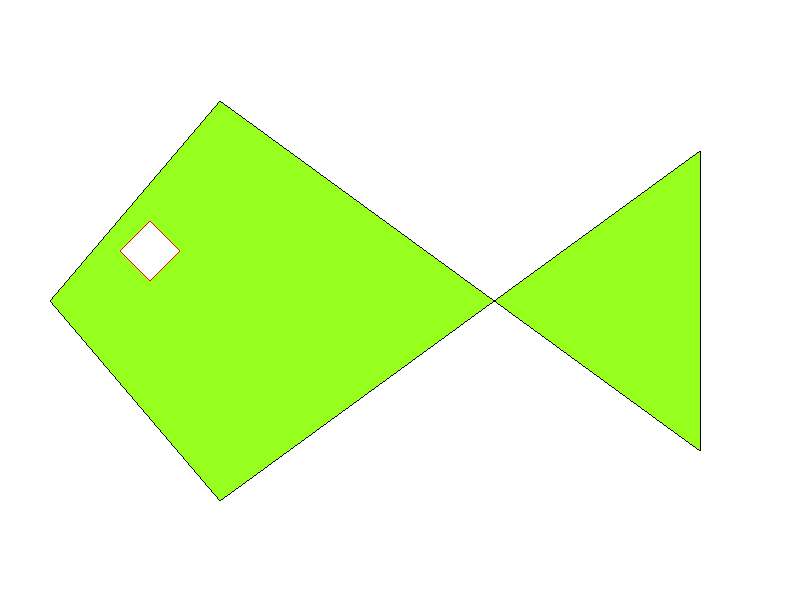
\includegraphics[width=\textwidth]{data/edit.png}}
  }
\ep
\end{uloha}

\begin{uloha}
  Uvažujme nasledovnú variáciu na tému Sierppińského koberca: máme parametre
  \prg!int x!, \prg!int d!,
  \prg!double i! a \prg!double f!. Chceme mať vzorku na obrázku rozmerov $x\times x$.
  Vzorka stupňa $d$  je štvorec so stranou dĺžky $ix$ umiestnený v strede obrázka.
  Navyše, ak $d>1$ tak v každom z rohov štvorca umiestnime vzorku stupňa $d-1$
  zmenšenú o faktor $f$ (a môže mať upravenú farbu). Napríklad pre
  hodnoty {\tt 1000 6 0.45 0.5} by vzorka mohla vyzerať takto:

  \ods{
\setlength{\fboxsep}{0pt}
  \centerline{\fbox{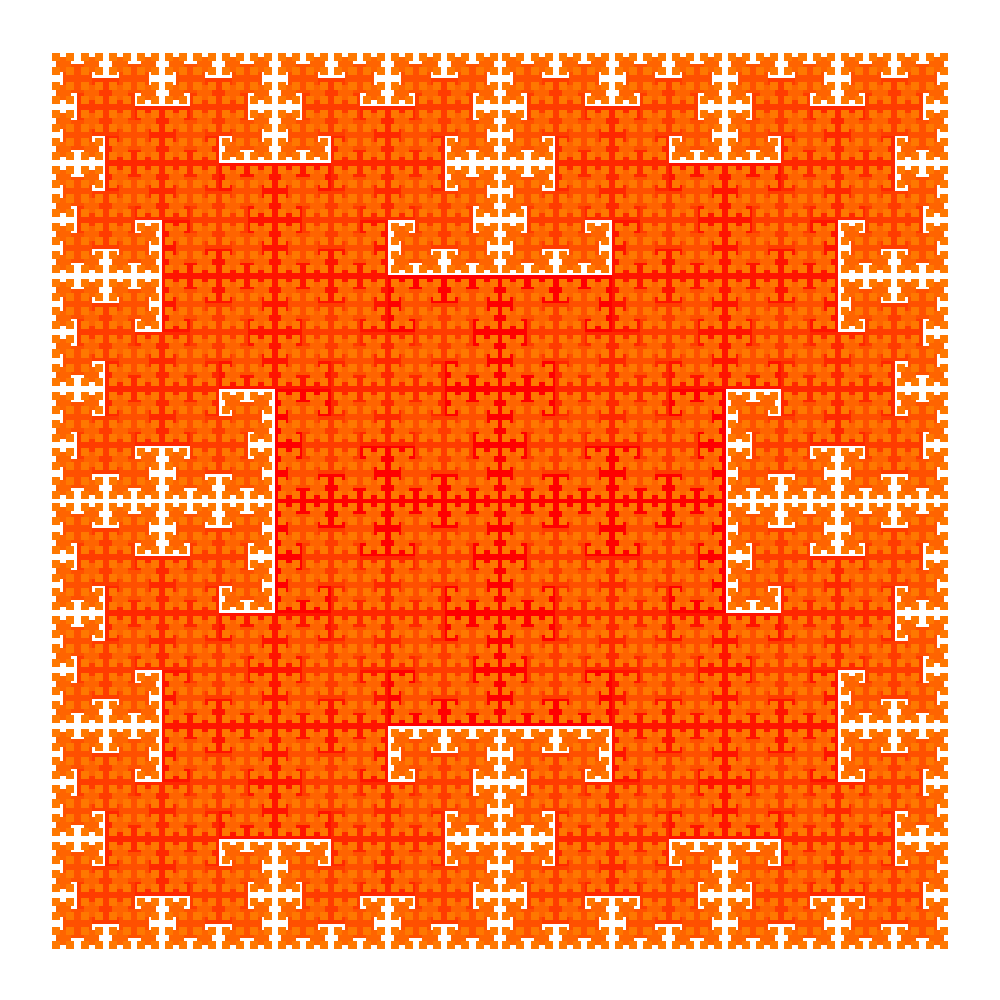
\includegraphics[width=0.4\textwidth]{data/qq.png}}}
}
  \ods

  Napíš program, ktorý načíta zo vstupu parametre {\tt x d i f} a vypíše postupnosť príkazov,
  na základe ktorej program z predchádzajúcej úlohy vykreslí 
  vzorku.
\end{uloha}

\subsection*{Odbočka: goniometrické funkcie $\sin$ a $\cos$}

Niekedy je dobré vedieť kresliť čiaru nie do konkrétneho bodu, ale pod istým uhlom.
Povedzme, že máme uhol $\alpha$ okolo bodu $P$. Urobíme si hocikoľko
kolmíc takto:

\ods
\centerline{
  \begin{tikzpicture}[scale=0.7]
  \def\an{30}
  \def\len{8}
  \def\ra{0.2}
  \draw[blue](\len,0) -- (0,0) node[anchor=north east]{$P$} -- (\an:\len+1);
  \draw[blue](1,0) arc (0:\an:1) node[midway,anchor=west]{$\alpha$};

  \foreach \x[count=\i] in {3.5,4.8,7} {
    \draw(\x,-1) -- (\x,5);
    \node[anchor=north east] at (intersection of 0,0--10,0 and \x,-1--\x,5) {$A_{\i}$};
    \node[anchor=south east] at (intersection of 0,0--\an:100 and \x,-1--\x,5) {$B_{\i}$};
    \draw (\x,\ra) arc (90:180:\ra);
    \filldraw (\x-\ra/3,\ra/3) circle (.3pt);
  }
\end{tikzpicture}}

\ods
Všetky trojuholníky $\triangle A_1PB_1$,  $\triangle A_2PB_2$, \ldots sú podobné: majú
všetky uhly rovnako veľké. Preto sa zachovávajú aj pomery strán: napr.\footnote{%
  znakom $\nrm{\cdot}$ označujem dĺžku
}
$\nrm{A_3P} = 2\nrm{A_1P}$, preto aj $\nrm{B_3P}=2\nrm{B_1P}$. To znamená, že 
$\frac{\nrm{A_3P}}{\nrm{B_3P}}=\frac{2\nrm{A_1P}}{2\nrm{B_1P}}=\frac{\nrm{A_1P}}{\nrm{B_1P}}$.
Inými slovami, pomer $\frac{\nrm{A_iP}}{\nrm{B_iP}}$ je stále rovnaký, nezáleží, ktorú kolmicu
$A_iB_i$ si zoberieme. Tento pomer závisí iba od uhla $\alpha$, a označuje sa $\cos(\alpha)$
({\em kosínus}). Podobne pomer $\frac{\nrm{B_iA_i}}{\nrm{B_iP}}$ závisí iba od $\alpha$
a označuje sa $\sin(\alpha)$ ({\em sínus}).

\ods
Na čo je dobré poznať hodnoty $\sin(\cdot)$ a $\cos(\cdot)$? Povedzme, že chceš zistiť,
aké súradnice má bod $B$, ktorý je od $[0,0]$ vo vzdialenosti $r$ pod uhlom $\alpha$:

\ods
\centerline{
  \begin{tikzpicture}[scale=4]
  \def\an{40}
  \def\ra{0.4ex}
    \draw[thin,dotted,step=0.5](-0.5,-0.5) grid (1,1);
    \draw(1.1,0) -- (0,0) node[anchor=north east]{$O=[0,0]$} -- (\an:1.1);

    \draw[red](1ex,0) arc (0:\an:1ex) node[midway,anchor=west]{$\alpha$};
    \draw[thin,gray](-35:1) arc (-35:125:1);

    \draw[-{>[length=3ex,width=1ex]},thin,gray] (0,0) -- (110:1) node[midway,anchor=east]
    {$r$};

    \coordinate (B) at (\an:1);
    \draw[red](0,0)--(B) node[midway,anchor=south east]{$r$};
    \node[right=3mm of B]  {$B=[x,y]$};

    \draw[blue] (B) -- (B|-0,0) coordinate (A) node[midway, anchor=west] {$y = \sin(\alpha)$};
    \node[anchor=north west] at (A) {$A$};
    
    \draw (A)+(0,\ra) arc (90:180:\ra);
    \filldraw (A)+(-\ra/3,\ra/3) circle (.1pt);

    \def\g{rgb:green,5;yellow,4;blue,2;black,3}
    \draw[thick,draw=\g](0,0)--(A) 
    node[midway,anchor=north]{\textcolor{\g}{$x = \cos(\alpha)$}};
\end{tikzpicture}}

\ods
Keď si z $B$ spravíš kolmicu, dostaneš pravouhlý $\triangle AOB$, pričom $\nrm{OA}=x$,
$\nrm{AB}=y$ sú hľadané súradnice bodu $B$. Z predchádzajúceho vieš, že 
$\cos{\alpha}=\frac{\nrm{OA}}{\nrm{OB}}=\frac{x}{r}$, preto $x=r\cos(\alpha)$.
Rovnako dostaneš $y=r\sin(\alpha)$.

\ods
Funcie \prg!sin! a \prg!cos! sú prístupné v knižnici, ktorá sa volá \prg!cmath!. 
Ich vstup ale nie je v stupňoch, ale v {\em radiánoch}. Ak obsah kruhu\footnote{%
  Urob si takýto pokus: zober si riešenie úlohy~\ref{uloha:kruh}
  a zrátaj v premennej {\tt S} počet čiernych pixelov. Na konci programu vypíš
  pomer čiernych pixelov k obsahu štvorca so stranou $r$, t.j. 
  \prg!(double)S / (double)(r * r)! Pre $r=10$ bol môj výsledok $3.05$, pre
  $r=500$ to už bolo $3.14128$ a pre $r=2450$ to bolo $3.14157$.

  \ods
\begin{tikzpicture}
\begin{axis}[
  % title={{\tt pi}},  
  width=\textwidth, 
  height=4cm,
  xlabel={$r$},
  scaled x ticks=false,
  scaled y ticks=false,
  domain=0:800,
  xmin=0,
  xmax=800,
  ymin=3.05,
  ymax=3.15,
  /pgf/number format/.cd,
  1000 sep={}
  %legend cell align={left},
  %legend pos = south east
]
  \addplot+[no markers,magenta,thick,dotted] {3.1415926535};
  \addplot+[no markers,blue!40!cyan] table 
  [y expr=\thisrow{pi}, x expr=\thisrow{n} ]{data/pi.dat};
\end{axis}
\end{tikzpicture}

Výsledok sa blíži k číslu $3.1415926535\cdots$, čo je hodnota $\pi$.
}
s polomerom 1 
označíme $\pi$, tak jeho obvod je $2\pi$. Radiány merajú uhol dĺžkou príslušného
oblúka na jednotkovej kružnici: celý kruh, čiže $360^\circ$ je $2\pi$ radiánov,
pravý uhol je $\pi/4$ radiánov atď. Vo všeobecnosti $d$ stupňov je $d\frac{2\pi}{360}$
radiánov. V knižnici {\tt cmath} je definovaná konštanta \prg!M_PI!, ktorá
dosť presne reprezentuje číslo $\pi$. Nasledovný program:

\ods
\vbox{
\begin{lstlisting}[] 
#include <cmath>  
#include <iostream>

using namespace std;

int main() {
  cout << 3*cos(M_PI / 2.0) << " " << 3*sin(M_PI / 2.0) << endl;
}
\end{lstlisting}
}


má vypísať súradnice bodu, ktorý je vo vzdialenosti $3$ pod uhlom $\pi/2$ (t.j. kolmo
hore), teda by sa malo vypísať {\tt 0 3}. V skutočnosti sa vypíše čosi ako 
{\tt 1.83697e-16 3}. Zápis {\tt 1.83697e-16} znamená $1.83697\cdot10^{-16}$, t.j. číslo
$0.000000000000000183697$. To je skoro nula, takže je to skoro správne. Nie je to presne nula,
lebo sa pri výpočte {\tt cos} prejavili problémy s presnosťou, ktoré si videl v 
predchádzajúcej časti.


\begin{uloha}
  Napíš program, ktorý na vstupe dostane čislo $n$ a vypíše postupnosť príkazov, na základe
  ktorých program z úlohy~\ref{uloha:editor} vykreslí vyplnený zelený pravidelný $n$-uholník.
\end{uloha}

\begin{uloha}
  Napíš program, ktorý na vstupe dostane číslo $n$ a $s$ a vyrobí príkazy pre program z 
  úlohy~\ref{uloha:editor}, ktorá nakreslia nasledovný útvar: zober si vrcholy pravidelného
  $n$-uholníka a spájaj ich čiarou s krokom $s$, t.j. spoj vrchol číslo $0$, 
  vrchol číslo $s$, vrchol číslo $2s$ a tak ďalej.
  Vnútro má byť vyfarbené žlto a vonkajšie cípy červeno. Napr. pre $n=7$, $s=3$ a pre
  $n=23$, $s=9$ sú tieto dva vzory:

  {
  \setlength{\fboxsep}{0pt}
  \bp\vspace{0pt}
  \centerline{\fbox{
\includegraphics[width=0.9\textwidth]{data/m.7.3.png}}}
  \ep\hfill
  \bp\vspace{0pt}
  \centerline{\fbox{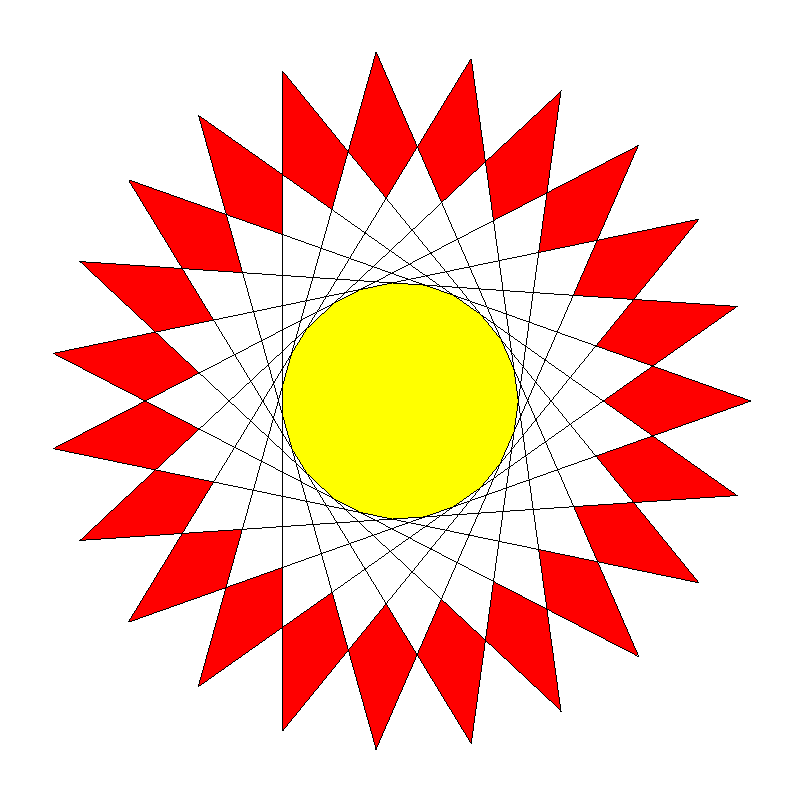
\includegraphics[width=0.9\textwidth]{data/m.23.9.png}}}
  \ep
  }
\end{uloha}

\vbox{
\begin{uloha}
  Korytnačia grafika pozostáva z postupnosti príkazov, každý na samostatnom riadku. 
  Príkazy sú takéto:
\def\tmp{\item \textcolor{magenta}}  
\begin{itemize}\itemsep=-1mm
    \tmp{{\tt i} {\em sirka vyska}} 
      (init) Toto je vždy prvý príkaz (a je v zozname iba
      raz). Nastaví rozmery obrázka. 
      \tmp{{\tt c} r g b} (color) Nastaví farbu na $\{r,g,b,255\}$.
    \tmp{{\tt u}} (pen up) Zdvihne pero -- nasledujúce posuny nekreslia.
    \tmp{{\tt d}} (pen down) Položí pero -- nasledujúce posuny kreslia.
    \tmp{{\tt f} x} (forward) Posunie sa dopredu o $x$.
    \tmp{{\tt l} a} (left) Otočí sa doľava o $a$ stupňov.
    \tmp{{\tt r} a} (right) Otočí sa doprava o $a$ stupňov.
    \tmp{{\tt s} meno} (save) Uloží obrázok a skončí.
\end{itemize}
Napíš program, ktorý načíta postupnosť príkazov korytnačej grafiky a vypíše
  postupnosť príkazov pre program z úlohy~\ref{uloha:editor}.
\end{uloha}
}

\ods
Na záver tejto časti skús rozšíriť korytnačiu grafiku o príkaz opakovania:

{\em
\def\tmp{\item \textcolor{magenta}}  
\begin{itemize}\itemsep=-1mm
      \tmp{{\tt R} cnt} (repeat) Blok príkazov po nasledujúci {\tt E} sa zopakuje
      {\em cnt} krát.
    \tmp{{\tt E}} (end) Koniec bloku opakovania.
\end{itemize}
}

\ods
Chceme, aby sa príkazy opakovania mohli vnárať, takže napr. program vľavo
urobí obrázok vpravo.

\begin{minipage}[t]{0.3\textwidth}\vspace{0pt}
\begin{verbatim}
i 700 700
R 24
R 4
f 100
r 90
E
l 15
E
c 0 50 200
R 8
u
f 250
d
R 36
f 50
l 180
f 50
l 10
E
u
l 180
f 250
l 225
E
s logo.png
\end{verbatim}
\end{minipage}
\hfill
\begin{minipage}[t]{0.7\textwidth}\vspace{0pt}{
  \setlength{\fboxsep}{0pt}
  \centerline{\fbox{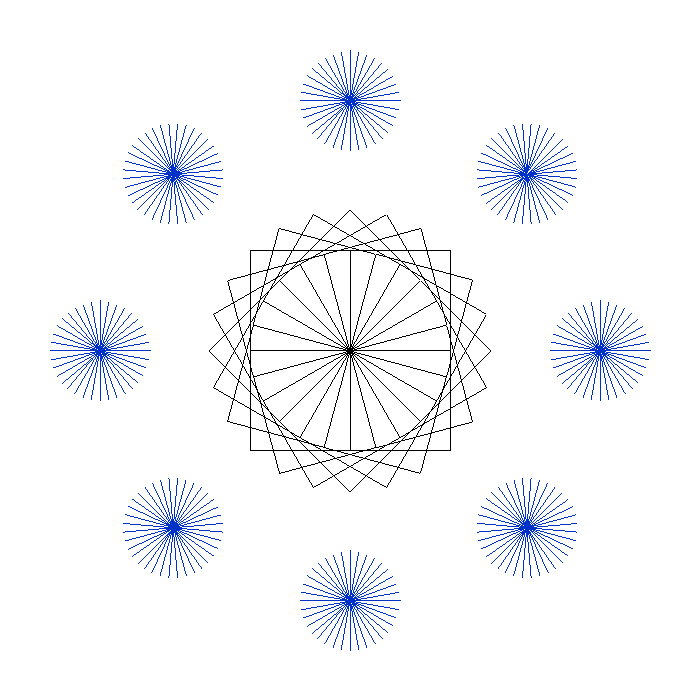
\includegraphics[width=\textwidth]{data/logo.png}}}
}
\end{minipage}

\ods
Na rozdiel od jednoduchšieho zadania bez cyklov, toto nemôžme riešiť tak, že 
príkazy čítame zo vstupu a priamo
vypisujeme príkazy pre kreslič, ale budeme si potrebovať všetky príkazy zapamätať.
Spravme si typ {\tt Prikaz}, v ktorom si budeme pamätať typ príkazu aj všetky
potrebné parametre (príkazy {\tt i} a {\tt s} ukladať nepotreujeme, {\tt i} je vždy
na začiatku a {\tt s} je na konci: keď načítame zo vstupu {\tt s}, tak vygenerujeme
všetky zapamätané príkazy a skončíme). Okrem parametrov si v príkaze
{\tt R} budeme potrebovať pamätať terajší počet opakovaní pri vykonávaní 
a v príkaze {\tt E} si budeme potrebovať zapamätať pozíciu, kde je príslušný
príkaz {\tt R}. Celý typ by mohol vyzerať napr. takto:

\ods
\vbox{
\begin{lstlisting}[] 
struct Prikaz {
  char t;       // typ prikazu
  int r, g, b;  // pre prikaz 'c'
  double x;     // genericky parameter pre prikazy 'l' 'r' 'f'
  int i, cnt;   // pre prikaz 'R'
  int addr;     // pre prikaz 'E'
};
\end{lstlisting}
}

\ods
Pri načítavaní vstupu si ukladáme príkazy do pamäte, pričom na príkazy {\tt R}
a {\tt E} použijeme zásobník ako v úlohe~\ref{uloha:zatvorky} na to, aby sme pre
každý príkaz {\tt E} našli zodpovedajúci príkaz {\tt R}. Začiatok programu z príkladu
by v poli vyzeral takto:

\ods
\centerline{
\begin{tikzpicture}[xscale=1.5,yscale=0.4]
    \def\cmd(#1)#2#3#4#5{
      \begin{scope}[shift={(#1,0)}]
        \draw (0,0) rectangle (1,5);
        \foreach \l [count = \i] in {addr,i,cnt,\ldots,t}{
          \node [anchor=south west] at (0,\i-1) {{\small\tt \l}};
        }
        \foreach \v [count = \i] in {#5,#4,#3,{},'#2'}{
          \node [anchor=south west] at (0.5,\i-1) {{\small\tt \textcolor{magenta}{\v}}};
        }
        \node [anchor=south] at (0.5,5) {$#1$};
      \end{scope}
      }

  \cmd(0)R{24}{0}{}
  \cmd(1)R{4}{0}{}
  \cmd(2)f{}{}{}
  \cmd(3)r{}{}{}
  \cmd(4)E{}{}{1}
  \cmd(5)l{}{}{}
  \cmd(6)E{}{}{0}
  \cmd(7)c{}{}{}
  \cmd(8)R{8}{0}{}
  \cmd(9)u{}{}{}
\end{tikzpicture}
}

\ods
Pri vyhodnocovaní programu budeme mať jednu globálnu premennú {\tt pc} (program counter),
v ktorej si budeme pamätať pozíciu práve vykonávaného príkazu. Štandardné príkazy vždy 
spracujeme (tak, že vypíšeme na výstup príslušný príkaz pre kreslič) a zvýšime {\tt pc}.
V príkaze {\tt R} len zvýšime hodnotu {\tt i}. V príkaze {\tt E} sa pozrieme na hodnotu
{\tt i} v príslušnom {\tt addr}: ak sa rovná {\tt cnt}, vynulujeme ju a zvýšime {\tt pc},
ak nie, skočíme na príkaz {\tt R}. Ak sa pole príkazov volá {\tt prog} a
v premennej {\tt n} máme počet príkazov, vyhodnocovanie by vyzeralo zhruba takto:

\ods
\vbox{
\begin{lstlisting}[] 
void execute() {
  int pc = 0;
  while (pc < n) {
    if (prog[pc].t == 'R') {
      prog[pc].i++;
      pc++;
    } else if (prog[pc].t == 'E') {
      int jmp = prog[pc].addr;
      if (prog[jmp].i == prog[jmp].cnt) {
        prog[jmp].i = 0;
        pc++;
      } else {
        pc = jmp;
      }
    } else if .... 

    // tu sa spracuju dalsie prikazy

  }
}


\end{lstlisting}
}


\begin{uloha}
  \label{uloha:logo}
  Naprogramuj korytnačiu grafiku s príkazmi cyklu.
\end{uloha}
\fi

%%%%%%%%%%%%%%%%%%%%%%%%%%%%%%%%%%%%%%%%%%%%%%%%%%%%%%%%%%%%%%%%%%%%%%%%%%%%
\if\sectxvii1
\section{Adresy a smerníky (pointre)}

Technicky je celá pamäť počítača jedno veľké pole núl a jednotiek. V skutočnosti má
adresu iba každý ôsmy bit (celá pamäť teda vyzerá ako pole \prg!unsigned char!).
Keby na adrese 1 bola premenná \prg!int c;!, na adrese 5
premenná \prg!char a! a na adrese 6 premenná \prg!char b;!
začiatok pamäte by mohol vyzerať takto:

\ods
\centerline{\begin{tikzpicture}[scale=0.2]
  \def\var#1[#2]#3#4{%
    \pgfmathsetmacro{\tmp}{#1+8*#2}
    \draw[#4] decorate[
       decoration={brace, amplitude=2ex}]{
       (#1,1.8) -- (\tmp,1.8) node [align=center,midway,anchor=south,yshift=2ex] {{\tt #3}}
        };
   \draw[#4,thick] (#1,0) rectangle (\tmp,1.5);

  }
  \foreach \v [count=\i] in {
    0,1,0,0,0,1,1,1,
    0,1,1,0,0,0,0,1,
    0,1,1,0,1,1,1,0,
    0,1,1,0,0,1,0,0,
    0,1,1,0,0,0,0,1,
    0,1,1,0,1,1,0,0,
    0,1,1,0,0,1,1,0,
    0,0,0,0,0,0,0,0,
    0,1
  }{
    \draw (\i,0) rectangle node [anchor=center] {{\scriptsize\ttfamily \v}} (\i+1,1.5);
  }

  \foreach \i in {0,...,8}{
    \pgfmathsetmacro{\x}{\i*8+1.5}
  \draw[dotted] (\x,-0.1) -- (\x,-3) 
  node[draw, anchor = north west]{\scriptsize{\tt \i}};
}

  \var{9}[4]c{orange!60!black}
  \var{41}[1]a{cyan!60!black}
  \var{49}[1]b{green!60!black}
\end{tikzpicture}}

\ods
To, že nejaká premenná je na nejakej adrese, nie je v pamäti nijak špeciálne označené, je 
na programe, aby pristupoval na správne miesta v pamäti. V pamäti je vždy okrem tvojho 
programu veľa ďalších vecí, takže keď sa proram spustí, operačný systém nájde v pamäti
voľné miesto a tvoj program bude používať adresy odtiaľ. Presná adresa premennej ti preto
sama osebe veľa nepovie, napriek tomu je užitočné ju vedieť. Až tak užitočné, že na to je
špeciálny operátor, \prg!&!. Ak máš premennú {\tt x}, tak \prg!&x! je jej adresa.
Skús si spustiť program:

\ods
\vbox{
\begin{lstlisting}[] 
#include <iostream>
using namespace std;

int c;
char a,b;

int main() {
  cout <<"adresa c: "<< (unsigned long)&c << endl;
  cout <<"adresa a: "<< (unsigned long)&a << endl;
  cout <<"adresa b: "<< (unsigned long)&b << endl;
} 
\end{lstlisting}
}

Vždy, keď ho spustíš, vypíšu sa iné čísla (tvoj program vždy dostane pridelenú
inú časť pamäte), ale môže to vyzerať napr. takto:

\begin{verbatim}
adresa c: 94082916049300
adresa a: 94082916049304
adresa b: 94082916049305
\end{verbatim}

V tomto prípade sa premenná {\tt c} uložila na adresu $94082916049300$ a zaberá 4 byty
(32 bitov). Za ňou, na adrese $94082916049304$ nasleduje premenná {\tt a}, ktorá zaberá
jeden byte, takže na nasledujúcej adrese $94082916049305$ je premenná {\tt b}.

\ods
Napriek tomu, že adresa je vždy číslo, operátor \prg!&! vracia v skutočnosti rôzne
typy. Pre každý typ {\tt T} (základný alebo vlastný
napr. \prg!int!, \prg!float!, \prg!Farba!,\ldots) existuje ďalší typ 
\cmd{adresa premennej typu {\tt T}} (hovorí sa aj {\em pointer na premennú typu {\tt T}}).
Tento nový typ sa označuje hviezdičkou pred menom premennej. Takže premenná typu \prg!int*! 
obsahuje adresu premennej, ktorá
je typu \prg!int!:


\ods
\vbox{
\begin{lstlisting}[] 
#include <iostream>
using namespace std;
int main() {
  int x = 258;       // premenna
  int *ax = &x;      // ok, ax je adresa x
  //float *err = &x;  --  error: cannot convert 'int*' to 'float*'
  float* fx = (float*)(&x);  // ok
}
\end{lstlisting}
}

V poslednom riadku som použil pretypovanie; {\tt fx} je adresa miesta, kde by mala byť
premenná typu \prg!float!, aj keď v skutočnosti je tam uložená premenná typu \prg!int! 
(konkrétne {\tt x}). Ešte raz treba zdôrazniť: premenná {\tt ax} je krabička, v ktorej
je uložené číslo adresy\footnote{%
  V nasledujúcom obrázku ťa zámerne trochu klamem, v premennej typu {\tt int} sa väčšinou
  jej 4 byty ukladajú v opačnom poradi (tzv. {\em little endian}), ale pre
  naše účely to stačí takto.
}, na ktorej je uložená krabička s menom {\tt x}:

\centerline{\begin{tikzpicture}[scale=0.2]
  \def\var#1[#2]#3#4{%
    \pgfmathsetmacro{\tmp}{2+#1+8*#2}
    \draw[#4] decorate[
       decoration={brace, amplitude=2ex}]{
       (2+#1,1.8) -- (\tmp,1.8) node [align=center,midway,anchor=south,yshift=2ex] {{\tt #3}}
        };
   \draw[#4,thick] (2+#1,0) rectangle (\tmp,1.5);

  }
  \foreach \v [count=\i] in {
    1,0,
    0,0,0,0,0,0,0,0,
    0,0,0,0,0,0,0,0,
    0,0,0,0,0,0,0,1,
    0,0,0,0,0,0,1,0,
    %
    0,0,0,0,0,0,0,0,
    0,0,0,0,0,0,0,0,
    0,0,0,0,0,0,0,1,
    0,0,1,1,1,0,1,1,
    0,1
  }{
    \draw (\i,0) rectangle node [anchor=center] {{\scriptsize\ttfamily \v}} (\i+1,1.5);
  }

  \foreach \i in {0,...,8}{
    \pgfmathsetmacro{\x}{\i*8+3.5}
    \pgfmathtruncatemacro{\l}{\i+315}
  \draw[dotted] (\x,-0.1) -- (\x,-3) 
  node[draw, anchor = north west]{\scriptsize{\tt \l}};
}

  \var{1}[4]{x = 258}{orange!60!black}
  \var{33}[4]{ax = 315}{cyan!60!black}
\end{tikzpicture}}


\ods Opačný operátor k \prg!&! je \prg!*!: ak \prg!ax! je premenná typu \prg!int*!, tak
\prg!*ax! je premenná, ktorá je uložená na adrese, ktorá je uložená v  {\tt ax}
(hovoríme, že premenná {\tt ax} {\em ukazuje na premennú} {\tt *ax}). 
Teraz je vidno, prečo je
dobré mať zvlášť typ adresy pre každý typ: keď sa vyhodnocuje výraz \prg!*ax!, procesor
sa pozrie do premennej {\tt ax}, nájde tam číslo (napr. 315), pozrie sa na adresu $315$
a predpokladá, že tam bude premenná typu \prg!pnt!. Pozrie sa preto na nasledujúce
4 byty a vráti príslušné číslo. V predchádzajúcom príklade by \prg!cout << *ax << endl;! vypísalo $258$.
\prg!*ax! je naozaj premenná, takže sa dá do nej aj priraďovať. Príkazy
\prg!x = 47;! a \prg!(*ax) = 47;! urobia to isté. Takže program

\ods
\vbox{
\begin{lstlisting}[] 
#include <iostream>
using namespace std;
int main() {
  int x = 258;       
  int* ax = &x;  // ax ukazuje na x   
  (*ax) = 47;    // *ax je x
  cout << x << endl;
}
\end{lstlisting}
}
vypíše 47.

\ods
Treba rozlišovať medzi hviezdičkou pri vyrábaní premennej (napr. \prg!int *a!), ktorá znamená
\cmd{pointer na typ int} a hviezdičkou pred menom premennej (typu pointer) vo výraze,
ktorá znamená \cmd{hodnota na adrese}. Skús prečítať nasledovný program:

\ods
\vbox{
\begin{lstlisting}[] 
#include <iostream>
using namespace std;

int main() {
  int a = 7, x = 6;  // a,x su premenne typu int
  int *b = &a;       // b ukazuje na a
  int **c = &b;      // c ukazuje na b
  int *d = *c;       // *c je premenna b, preto tento prikaz
                     // je rovnaky ako int* d = b;
  **c = 18;
  b = &x;            // teraz b ukazuje na x
  **c = 42;          
  cout << a << " " << x << endl;
}
\end{lstlisting}
}

Po prvých štyroch riadkoch by to v pamäti mohlo vyzerať ako na obrázku vľavo.
V príkaze \prg!**c=18;! je \prg!*c! premenná \prg!b! a \prg!*b! je premenná \prg!a!,
preto sa do premennej \prg!a! zapíše 18.
Nasledujúci príkaz \prg!b=&x! spôsobí, že v {\tt b} bude uložená adresa {\tt x} ako na 
obrázku vpravo. Preto v príkaze \prg!**c=42! je \prg!*c! premenná \prg!b!
a \prg!*b! je premenná \prg!x!, takže program vypíše {\tt 18 42}.

\ods
\def\var(#1)#2#3#4{%
  \draw (0,0.5-#1)  node[anchor=east]{{\tt #3}};
  \draw (0.2,-#1) rectangle node[align=center]{{\tt #2}} (1.2,1-#1);
  \draw (1.4,0.5-#1) node[anchor=west]{\textcolor{magenta}{\tt #4}};
}

\def\ptr(#1,#2)[#3] {
  \draw[blue,-{>[length=4pt,width=2.5pt]}] (1.7,0.5-#1) to[out=#3,in=-#3] (1.7,0.5-#2);
}

\bp
\begin{tikzpicture}[yscale=0.4,xscale=1.4]
  \node[anchor=east] at (0,0.8){{\em adresa}};
  \foreach \val/\addr/\name[count=\i] in {7/42380/a,6/42384/x,42380/42388/b,
     42388/42396/c,42380/42404/d}  {
    \var(\i){\val}{\addr}{\name}
  }
  \draw(0,0.5-6) node[anchor=east]{{\tt 42412}};
  \draw[draw=none] (0.2,-6) rectangle node[align=center]{{\tt \ldots}} (1.2,1-6);
  \ptr(3,1)[75]
  \ptr(4,3)[60]
  \ptr(5,1)[65]
\end{tikzpicture}
\ep
\hfill
\bp
\begin{tikzpicture}[yscale=0.4,xscale=1.4]
  \node[anchor=east] at (0,0.8){{\em adresa}};
  \foreach \val/\addr/\name[count=\i] in {18/42380/a,6/42384/x,42384/42388/b,
     42388/42396/c,42380/42404/d}  {
    \var(\i){\val}{\addr}{\name}
  }
  \draw(0,0.5-6) node[anchor=east]{{\tt 42412}};
  \draw[draw=none] (0.2,-6) rectangle node[align=center]{{\tt \ldots}} (1.2,1-6);
  \ptr(3,2)[60]
  \ptr(4,3)[60]
  \ptr(5,1)[65]
\end{tikzpicture}
\ep

\ods
S pomocou pointrov môžeš mať funkciu, ktorá ako keby menila svoje parametre.
Porovnaj tieto dva programy:

\ods
\bp
\vbox{
\begin{lstlisting}[] 
#include <iostream>
using namespace std;

void pridaj(int a) { 
  a = a + 1; 
}

int main() {
  int x = 7;
  pridaj(x);
  cout << x << endl;
} 
\end{lstlisting}
}
\ep
\hfill
\bp
\vbox{
\begin{lstlisting}[] 
#include <iostream>
using namespace std;

void pridaj(int *a) {
  (*a) = (*a) + 1;
}

int main() {
  int x = 7;
  pridaj(&x);
  cout << x << endl;
}
\end{lstlisting}
}
\ep

V ľavom programe sa vyrobí svet funkcie {\tt main} a v ňom premenná {\tt x}. Pri
volaní funkcie {\tt pridaj} sa vyrobí nový svet s premennou {\tt a} a nastaví sa jej
hodnota na $7$. Potom sa vykoná funkcia {\tt pridaj}, takže v premennej {\tt a}
bude $8$. Svet funkcie {\tt pridaj} potom zanikne a v {\tt main} sa vypíše hodnota 
{\tt x}, t.j. 7. V pravom programe sa vyrobí svet funcie {\tt pridaj}, ale 
premenná {\tt a} sa nastaví na adresu premennej {\tt x} (premenná {\tt x} je vo svete 
funkcie {\tt main}, ale svety a premenné sú vec programu a kompilátora; pri prístupe
do pamäte vo výslednej binárke nehrajú rolu).
Preto vo svete {\tt pridaj}  výraz {\tt *a} označuje premennú {\tt x} zo sveta funkcie {\tt main}
a funkcia {\tt pridaj} zvýši hodnotu {\tt x} o 1. Keď svet {\tt pridaj}
zanikne, zanikne premenná {\tt a}, ale hodnota {\tt x} ostane zmenená.

\ods
\def\var(#1)#2#3#4{%
  \draw (0,0.5-#1)  node[anchor=east]{{\tt #3}};
  \draw (0.2,-#1) rectangle node[align=center]{{\tt #2}} (1.2,1-#1);
  \draw (1.4,0.5-#1) node[anchor=west]{\textcolor{magenta}{\tt #4}};
}

\def\ptr(#1,#2)[#3] {
  \draw[blue,-{>[length=4pt,width=2.5pt]}] (1.7,0.5-#1) to[out=#3,in=-#3] (1.7,0.5-#2);
}

\def\kon(#1)#2{ \draw(0,0.5-#1) node[anchor=east]{{\tt #2}};
  \draw[draw=none] (0.2,-#1) rectangle node[align=center]{{\tt \ldots}} (1.2,1-#1);
}

\def\world(#1)#2#3{
  \draw[thick,#3](-1,-#1) -- (2,-#1) node[anchor=west]{{\tt #2}};
}
\bp
\begin{tikzpicture}[yscale=0.4,xscale=1.4]
  \node[anchor=east] at (0,0.8){{\em adresa}};
  \world(0){main}{orange}
  \world(1){pridaj}{blue!70!gray}

  \foreach \val/\addr/\name[count=\i] in {7/873200/x,8/873204/a}  {
    \var(\i){\val}{\addr}{\name}
  }
  
  \kon(3){873208}
\end{tikzpicture}
\ep
\hfill
\bp
\begin{tikzpicture}[yscale=0.4,xscale=1.4]
  \node[anchor=east] at (0,0.8){{\em adresa}};
  \world(0){main}{orange}
  \world(1){pridaj}{blue!70!gray}

  \foreach \val/\addr/\name[count=\i] in {8/873200/x,837200/873204/a}  {
    \var(\i){\val}{\addr}{\name}
  }
  \ptr(2,1)[70]
  \kon(3){873208}
\end{tikzpicture}
\ep

\ods
S pointrami sa dajú robiť aj aritmetické operácie, ale trochu inak ako s normálnymi
číslami. Ak k premennej typu pointer pripočítaš 1, zväčší sa o veľkosť typu, na ktorý
ukazuje (v prípade \prg!int! je to 4). Veľkosť typu sa dá zistiť pomocou príkazu
\prg!sizeof!. V poli sú prvky uložené za sebou, takže napr. program

\vbox{
\begin{lstlisting}[] 
#include <iostream>
using namespace std;

int main() {
  int a[2] = {12, 35};
  int *x = &(a[0]);
  cout << *x << " " << *(x + 1) << endl;
  cout << (unsigned long)x << " + " << sizeof(int) << " = "
       << (unsigned long)(x + 1) << endl;
}
\end{lstlisting}
}

mi vypísal

\begin{verbatim}
12 35
140727139715200 + 4 = 140727139715204
\end{verbatim}

Pri práci s pointrami si treba dávať pozor na to, aby vždy ukazovali do pamäte,
ktorá patrí tvojmu programu. Môžeš napríklad napísať \prg!int *a = (int*)856;!
a nič zlé sa nestane. Ale ak by si potom chcel urobiť \prg!*a = 3;!, program skončí
s hláškou {\tt Segmentation fault}: pamäť na adrese 856 ti nepatrí. Je dobrý zvyk
do pointrov, ktoré zatiaľ neukazujú na nič rozumné, priradiť 0 (adresa 0 ti celkom
isto nepatrí) a pred použitím urobiť test. Môžeš napísať \prg!int *a = 0;!, alebo
\prg!int *a = NULL;! alebo \prg!int *a = nullptr;!, všetky tri spravia v konečnom 
dôsledku to isté.

\ods
Samozrejme, pointer môže ukazovať aj na vlastné typy a dokonca aj na polia.
To môže byť trochu zamotané. Napr.

\vbox{
\begin{lstlisting}[] 
int a, b, c;
int *p[3] = {&a, &b, &c};

*(p[0]) = 5;
*(p[1]) = 25;
*(p[2]) = 225;

cout << a << " " << b << " " << c << endl;
\end{lstlisting}
}

vyrobí trojprvkové pole {\tt p}, ktorého prvky budú pointre na premenné typu \prg!int!
a naplní ho pointrami na premenné {\tt a, b, c}. Preto potom \prg!p[0]! je pointer
na premennú \prg!a! a teda \prg!*(p[0]) = 5;! priradí 5 do premennej {\tt a}
a program vypíše {\tt 5 25 225}. Zápis \prg!int *p[3]! čítaš najprv od 
názvu premennej doprava
a potom doľava zvyšok: \cmd{pole dĺžky 3, ktorého prvky sú pointre na int}.
Ak napíšeš \prg!int (*p)[3]!, znemená to \cmd{pointer na pole dĺžky 3,
ktorého prvky sú int}:

\vbox{
\begin{lstlisting}[] 
int a[3] = {1, 2, 3};
int(*p)[3] = &a;

cout << (*p)[1] << endl;
\end{lstlisting}
}

Ako by si zapísal pole dĺžky 2, ktorého prvky sú polia dĺžky 3? \prg!int a[2][3]!
Pripomína ti to niečo? Presne tak, je to dvojrozmerné pole. Dvojrozmerné pole
je vlastne pole riadkov, ktorého prvky sú polia stĺpcov. Preto môžeš mať

\vbox{
\begin{lstlisting}[] 
int a[2][3] = {{1, 2, 3}, {4, 5, 6}};
int(*p)[3] = &(a[0]);

cout << (*(p+1))[1] << endl;
\end{lstlisting}
}

V tomto prípade {\tt a} je pole dĺžky 2, ktorého prvky sú trojprvkové polia,
preto {\tt a[0]} je trojprvkové pole.
{\tt p} je pointer na trojprvkové pole, preto môžeš napísať \prg!p=&(a[0])!.
Potom \prg!p+1! ukazuje do pamäte o 12 bytov ďalej (\prg!sizeof(int[3])! je 12).
Prvky v poli sú uložené za sebou, preto 
ak \prg!p! ukazuje na \prg!a[0]!, tak \prg!p+1! ukazuje na \prg!a[1]!.
Napokon \prg!*(p+1)! je to isté, čo \prg!a[1]!, preto \prg!(*(p+1))[1]! vypíše 5.

\fi

%%%%%%%%%%%%%%%%%%%%%%%%%%%%%%%%%%%%%%%%%%%%%%%%%%%%%%%%%%%%%%%%%%%%%%%%%%%%
\if\sectxviii1
\section{Polia revealed}

Hovoril som ti, že pole nie je premenná, ale veľa premenných, a preto sa
správa zvláštne (napr. si nesmel posielať pole ako parameter do funkcie,
nesmel si priraďovať a pod.). V skutočnosti je pole konštatný\footnote{%
S označením \prg!const! sme sa už stretli v tvare \prg!const int n = 100;!: 
ak ho napíšeš pred definíciu premennej,
znamená to, že premenná sa už potom nesmie meniť. 
Podobne môže byť \prg!const int *a = &x;!
}pointer.
Keď napíšeš \prg!int a[10];! vyrobí sa v pamäti 10 premenných typu \prg!int!
a {\tt a} je \prg!const! pointer na prvú z nich. Označenie indexu {\tt [ ]}
je v skutočnosti iba skratka za výraz s hviezdičkou: \prg!a[i]! znamená
\prg!*(a+i)! pre hocijaký pointer {\tt a}. Rôzne spôsoby prístupu k
prvkom poľa sú v nasledujúcom programe:

\vbox{
\begin{lstlisting}[] 
#include <iostream>
using namespace std;

int main() {
  int a[10];
  int *b, *c;
  int i;
  // a = b; -- chyba, a je const
  c = a + 1;  // c ukazuje na a[1]

  b = a;  // b ukazuje na a[0]
  for (i = 0; i < 10; i++) {
    *b = i + 1;  // *b zapisuje do pola a
    b = b + 1;   // presun b na dalsi prvok pola
  }

  cout << a[0] << endl;
  for (i = 0; i < 9; i++)
    cout << c[i] << endl;  // c ukazuje na a[1], preto
                           // c[i] je a[i+1]

  *(a + 5) = 14;                // *(a+5) je a[5]
  for (b = a; b < a + 10; b++)  // k b sa da pripocitavat cislo aj takto
    cout << *b << " ";
  cout << endl;
}
\end{lstlisting}
}

\ods
Teraz by malo byť jasné, ako sa dá posielať pole ako parameter do funkcie: stačí,
aby bol typu pointer. Treba si ale vždy poslať aj veľkosť poľa ako samostatný parameter:

\vbox{
\begin{lstlisting}[] 
#include <iostream>
using namespace std;

void napln_pole(int n, int *a) {
  int i;
  for (i = 0; i < n; i++)
    a[i] = i * i;
}

int main() {
  int a[10];
  napln_pole(10, a);
  int i;
  for (i = 0; i < 10; i++)
    cout << a[i] << " ";
  cout << endl;
}
\end{lstlisting}
}

Tento program vypíše {\tt 0 1 4 9 16 25 36 49 64 81}. Len pripomeniem: ak by si v tomto
programe zmenil riadok \prg!int a[10];! na \prg!int a[3];!, program by fungoval rovnako,
akurát, že vo funkcii {\tt napln\_pole} by sa zapisovalo aj do pamäte, ktorá nebola
rezervovaná poľom {\tt a}. Ak sú tam nejaké premenné tvojho programu (napr. {\tt i}), 
prepíšu sa. Ak tá
pamäť tvojmu programu nepatrí, príde náš priateľ {\tt segfault}.


\ods
Dvojrozmerné pole je pole, ktorého prvkami sú polia. Preto ak máš \prg!int a[2][3]!,
tak {\tt a} je (konštatný) pointer na trojprvkové pole typu \prg!int!. Preto 
\prg!*(a+1)! je to isté, čo \prg!a[1]!, čiže trojprvkové pole typu \prg!int!
(t.j. môžeš napíať \prg!int *q = *(a+1);! a potom \prg!q! bude ukazovať na
prvý prvok poľa \prg!a[1]!, čiže na druhý riadok poľa \prg!a!).
Z toho celého vyplýva, že dvojrozmerné pole je v pamäti vlastne jednorozmerné
pole uložené rovnako, ako sme to mali v kapitole~\ref{sect:2dpolia}.
Na to, aby si k nemu tak mohol pristupovať, treba ho pretypovať, takže môžeš
napísať \prg!int *p = (int *)a;!. To je zároveň aj najjednoduchší spôsob, ako
posielať dvojrozmerné pole ako parameter do funkcie.

\vbox{
\begin{lstlisting}[] 
int main() {
  int a[2][3];
  int i, j, k = 1;

  for (i = 0; i < 2; i++)      // naplnime pole po riadkoch 
    for (j = 0; j < 3; j++) {
      a[i][j] = k;
      k++;
    }

  int *q = *(a + 1);           // q ukazuje na druhy riadok
  for (int i = 0; i < 3; i++) 
    cout << q[i] << endl;

  int *p = (int *)a;          // pohlad na a ako na 1D pole 
  for (i = 0; i < 6; i++) 
    cout << p[i] << " ";
  cout << endl;
} 
\end{lstlisting}
}


\ods Malá odbočka: mechanizmus posielania parametrov pointrami sa používa aj v iných 
programovacích jazykoch, ale častokrát ``pod kapotou''. Napríklad python posiela
základné typy ako parametre (tzv. {\em volanie hodnotou}), ale na zoznamy a iné zložité
typy posiela pointer (tzv. {\em volanie referenciou}). Pythonovský program

\vbox{
\begin{lstlisting}[language=python] 
def zelena(x):
    x = 42

def modra(x):
    x[0] = 42

a = 1
zelena(a)
print(a)

b = [1, 2, 3]
modra(b)
print(b)
\end{lstlisting}
}

vypíše

\begin{verbatim}
1
[42, 2, 3]
\end{verbatim}

Do funkcie {\tt zelena} sa poslalo číslo, preto sa menila hodnota lokálnej premennej
vo svete funkcie {\tt zelena} (ktorá spolu s jej svetom zanikla), do funkcie {\tt modra}
sa poslal pointer na zoznam {\tt b}. Tento spôsob volania dáva zmysel, lebo väčšinou je to
presne to, čo chceš, ale pre začínajúcich programátorov to niekedy môže byť mätúce.
Koniec malej odbočky.

\ods Vyriešili sme, ako posielať polia ako parametre, ale stále nám ostáva problém 
s globálnymi poľami. Pamätáš sa, že keď sme pri kreslení obrázkov chceli mať globálne
pole, museli sme ho vyrobiť tak, aby už v čase kompilácie bola známa jeho veľkosť. 
Riešili sme to tak, že sme pole spravili dostatočne veľké a používali z neho iba 
tak veľký kus, ako sme potrebovali. Toto evidentne nie je najlepší prístup. 
Lepšie riešenie je tzv. {\em dynamická alokácia}: príkaz \prg!new int[100];! 
vyhradí v odľahlom kúte pamäte miesto na 100 premenných typu \prg!int! a vráti pointer
naň. Toto miesto je vyhradené pre tvoj program, ale vrátený pointer je jediný spôsob,
ako sa k tej pamäti dostať: ak si ho neuložíš do premennej (alebo ju neskôr zabudneš),
pamäť stále ostane vyhradená pre tvoj program, ale ten sa k nej už nikdy nebude môcť dostať.
Ak už alokovanú pamäť nepotrebuješ, treba ju vrátiť systému príkazom \prg!delete[]!. Treba
byť opatrný, lebo to, či je pamäť vyhradená, alebo nie, nijak nevidno. Dobrý zvyk 
je hneď po volaní \prg!delete[]! priradiť do odalokovanej premennej \prg!nullptr!.

\vbox{
\begin{lstlisting}[] 
#include <iostream>
using namespace std;

int *a = (int *)12345;

void rob_nieco() {
  int i;
  for (i = 0; i < 100; i++) a[i] = 42;
}   

void vypis(int x) { cout << x << ": " << (unsigned long)a << endl; }
  
int main() {
  vypis(1);
  a = new int[100];
  vypis(2);     // a ukazuje na pridelenu pamat
  rob_nieco();  // v poriadku, pisem do svojej pamate
  delete[] a;   // pridelena pamat sa oznacila ako volna
  vypis(3);     // hodnota a sa nezmenila, stale ukazuje na to iste miesto,
                // ale ta pamat ti uz nepatri
  // rob_nieco();  -- !! toto by bol problem - system medzitym mohol 
                // tu pamat dat niekomu inemu
}
\end{lstlisting}
}

Tento program vypíše napr.
\begin{verbatim}
1: 12345
2: 94751025169088
3: 94751025169088
\end{verbatim}

 Pri priraďovaní si treba dávať pozor, 
hlavne ak je pointer na dynamicky alokovanú pamäť súčasť zloženého typu, napr.

\vbox{
\begin{lstlisting}[] 
struct Kvak {
  int *a, b, c[2];
};
\end{lstlisting}
}

Ak mapíšeš

\begin{lstlisting}[] 
Kvak x, y;
x.a = new int[100];
y.a = new int[100];
\end{lstlisting}

a ešte ponastavuješ ďalšie hodnoty, môže to v pamäti vyzerať takto:

\ods
\def\var(#1)#2#3{%
  \draw (0.2,-#1) rectangle node[align=center](v#1) {{\tt #3}} (1.2,1-#1);
  \draw (0,0.5-#1) node[anchor=east]{\textcolor{magenta}{\tt #2}};
}

\def\ptr(#1,#2)[#3] {
  \draw[blue,-{>[length=4pt,width=2.5pt]}] (1.7,0.5-#1) to[out=#3,in=-#3] (1.7,0.5-#2);
}

\def\world(#1)#2#3{
  \draw[thick,#3](-1,-#1) -- (2,-#1) node[anchor=west]{{\tt #2}};
}

\def\kon(#1){ 
  \draw[draw=none] (0.2,-#1) rectangle node[align=center]{{\tt \ldots}} (1.2,1-#1);
}
  
\def\godot#1{\filldraw[blue,scale=0.6](#1) circle (0.4ex and 1.4ex);}

\begin{tikzpicture}[yscale=0.4,xscale=1.4]

  \var(0){x.a}{}
  \var(1){x.b}{1}
  \var(2){x.c[0]}{2}
  \var(3){x.c[1]}{3}
  \var(4){y.a}{}
  \var(5){y.b}{4}
  \var(6){y.c[0]}{5}
  \var(7){y.c[1]}{6}
  \world(-1){x}{orange}
  \world(3){y}{olive}
  \kon(8)

  \coordinate (a1) at (3,-0.5);
  \coordinate (a2) at (3,-4.5);

  \foreach \f/\t/\l in {v0/a1/{},v4/a2/{inde\ }}{
  \godot{\f}
  \draw[blue,-{>[length=8pt,width=5pt]}] (\f) to [out=0,in=180] (\t);
  \draw (\t)++(0,-0.5) rectangle node[align=center]{400 bytov niekde \l v pamäti} ++(5,1);
  }
\end{tikzpicture}

keď potom napíšeš \prg!y=x!, stane sa toto:

\begin{tikzpicture}[yscale=0.4,xscale=1.4]

  \var(0){x.a}{}
  \var(1){x.b}{1}
  \var(2){x.c[0]}{2}
  \var(3){x.c[1]}{3}
  \var(4){y.a}{}
  \var(5){y.b}{1}
  \var(6){y.c[0]}{2}
  \var(7){y.c[1]}{3}
  \world(-1){x}{orange}
  \world(3){y}{olive}
  \kon(8)

  \coordinate (a1) at (3,-0.5);
  \coordinate (a2) at (3,-4.5);

  \foreach \f/\t/\l in {v0/a1/{},v4/a2/{inde\ }}{
  \godot{\f}
  \draw (\t)++(0,-0.5) rectangle node[align=center]{400 bytov niekde \l v pamäti} ++(5,1);
  }

  \draw[blue,-{>[length=8pt,width=5pt]}] (v0) to [out=0,in=180] (3,-0.35);
  \draw[blue,-{>[length=8pt,width=5pt]}] (v4) to [out=0,in=180] (3,-0.65);
\end{tikzpicture}

Navždy si stratil 400 bytov pamäte a navyše ak napíšeš \prg!delete[] x.a; delete[] y.a;!
program zhavaruje s chybou

\begin{verbatim}
free(): double free detected in tcache 2
Aborted
\end{verbatim}

lebo si dvakrát odalokovával tú istú pamäť (aj keď si sa k nej dostal z iných pointrov).

\begin{uloha}
  Npaíš funkciu, kotrá ako parametre dostane číslo $n$ a pointer na  pole $n$
  čísel a toto pole v pamäti otočí. Napr. ak pred volaním bolo $n=5$
  a v poli boli čísla {\tt 1 2 3 4 5} po volaní tam bude {\tt 5 4 3 2 1}.
\end{uloha}

\begin{uloha}
  \label{uloha:arraycopy}
  Napíš funkciu, ktorá ako parametre dostane číslo $n$ a pointer na pole $n$
  čísel a toto pole skopíruje (t.j. vráti pointer na iné pole, v ktorom budú
  tie isté prvky).
\end{uloha}

\begin{uloha}
  Napíš funkciu, kotrá ako parametre dostane číslo $n$, pointer na  pole $n$
  čísel a číslo $k$ a pole v pamäti cyklicky posunie o $k$ miest.
  Napr. ak $n=5$, $k=2$ a pole bolo {\tt 1 2 3 4 5}, tak po volaní funkcie
  pole bude {\tt 3 4 5 1 2}.
\end{uloha}

\begin{uloha}
  \label{uloha:primetest}
  Napíš funkciu, ktorá dostane parameter $n$ a vráti pointer na dynamicky alokované
  pole, v ktrorm bude prvých $n$ prvočísel\footnote{%
    Prvočíslo je číslo $p$, ktoré nemá iných deliteľov ako 1 a $p$. Inými slovami
    \prg~p\%i != 0~ pre všetky $i<p$. Ak to chceš jemne vylepšiť, premysli si,
    že ak má číslo $a$ nejakého deliteľa, tak má aj deliteľa veľkosti 
    nanajvýš $\sqrt{a}$. Ak na začiatku napíšeš \prg!#include<cmath>!, môžeš
    použiť funckiu \prg!sqrt(x)! na výpočet $\sqrt{x}$ (vracia typ double).
    }.
\end{uloha}

\begin{uloha}
  \label{uloha:merge}
  Napíš funkciu, ktorá dostane ako parametre dve utriedené polia veľkostí $n$ a $m$
  (t.j. dostane $n$, $m$ a dva pointre) a vyrobí utriedené pole dĺžky $n+m$, 
  ktoré obsahuje prvky z oboch vstupných polí.
\end{uloha}

\begin{uloha}
  \label{uloha:mergesort}
  Napíš funkciu, ktorá dostane ako parameter $n$ a dynamicky alokované pole
  dľžky $n$ a utriedi ho pomocou algoritmu {\em Merge Sort}. Algoritmus {\em Merge
  Sort} je rekurzívny algoritmus, ktorý funguje takto: pole dĺžky $1$ je utriedené,
  netreba nič robiť. Ak má pole dĺžku aspoň 2, rozdeľ ho na dve polovice (t.j.
  vyrob si nové polia správnej dĺžky, prekopíruj do nich prvky z pôvodného poľa)
  a rekurzívne obe utrieď. Potom použi algoritmus z úlohy~\ref{uloha:merge} na to,
  aby si vyrobil výsedné pole (nezabudni vrátiť pamäť z pomocných polí).
\end{uloha}

\begin{uloha}
  \label{uloha:sortbody}
  Majme typ \prg!struct Bod{float x,y;};! Napíš funkciu, ktorá ako parameter
  dostane pole bodov a utriedi ho\footnote{napr. pomocou algoritmu {\em Insertion Sort}
  z kapitoly~\ref{sect:zlozitost}} podľa $x$-ovej súradnice.
\end{uloha}

\begin{uloha}
  Na vstupe je číslo $n$, a pole $n$ čísel {\tt t[0]},\ldots,{\tt t[n-1]}, ktoré 
  predstavujú časované bomby: {\tt i}-ta bomba vybuchne po {\tt t[i]} sekundách.
  Pyrotechnik vie každú sekundu zneškodniť jednu bombu. Napíš program, ktorý
  zistí, či sa mu podarí zneškodniť všetky bomby. Napr. pre vstup {\tt 9 3 2 5 2} 
  sa mu to podarí: v prvej sekunde zneškodní poslednú bombu, preto v druhej sekunde
  budú časovače na bombách ukazovať {\tt 8 2 1 4 $\times$}. Pyrotechnik akurát včas zneškodní
  bombu číslo $2$, takže bude stav {\tt 7 1 $\times$ 3 $\times$}, opäť v poslednej
  sekunde zneškodní bombu č.1: {\tt 6 $\times$ $\times$ 2 $\times$} a posledné dve bomby
  zneškodní s prehľadom. Pre vstup {\tt 3 4 3 7 1 3} sa mu to ale nepodarí.
\end{uloha}

\fi

%%%%%%%%%%%%%%%%%%%%%%%%%%%%%%%%%%%%%%%%%%%%%%%%%%%%%%%%%%%%%%%%%%%%%%%%%%%%
\if\sectxix1
\section{Zásobník ako vlastný typ}

V kapitole~\ref{sect:stack} sme používali zásobník tak, že sme mali pole fixnej
veľkosti a jednu premennú, ktorá udávala aktuálny počet prvkov v zásobníku. Keby sme chceli
mať viac zásobníkov, mali by sme viac polí a viac premenných. Aby sme v tom udržali
poriadok, je dobré spraviť si vlastný typ, kde budú obe veci pokope, napr.

\vbox{
\begin{lstlisting}[] 
#include <iostream>
using namespace std;

const int N = 100000;

struct Stack {
  int a[N], n;
};
  
int main() {
  Stack s1, s2;

  s1.n = 0;
  s2.n = 0;

  // pridaj prvok
  s1.a[n]=1;
  s1.n++;
}
\end{lstlisting}
}

\ods
Takáto definícia má dva problémy: vždy, keď vyrobíme zásobník, vyhradí sa v pamäti
veľké pole, aj keby sme dopredu vedeli, že budeme potrebovať menej. Druhý problém je,
že na pridanie prvku treba dva príkazy, čo pri častom používaní môže byť neprehľadné.
Prvý problém vyriešime dynamickou alokáciou: zásobník si bude pamätať, aké veľké pole
má alokované a na začiatku ho inicializujeme. Inicializáciu aj pridanie prvku zariadime 
funkciami. Tieto musia ako parameter dostávať pointer na zásobník, aby mohli meniť jeho 
premenné\footnote{%
Keby dostali ako parameter namiesto \prg!Stack *s! iba \prg!Stack s!, pri volaní
funkcie sa zásobník (t.j. premenné \prg!a, n, max!)  
skopíruje do lokálneho sveta funkcie, tam sa zmení
a po skončení volania spolu so svetom zanikne. Dynamicky alokované pamäť by ostala,
ale pointer na ňu bu sa stratil. To nie je to, čo chceme.
}.


\begin{lstlisting}[] 
#include <iostream>
using namespace std;

struct Stack {
  int *a, n, max;
};
  
void resize(Stack *s, int max) {
  (*s).a = new int[max];
  (*s).max = max;
  (*s).n = 0;
} 

bool push(Stack *s, int x) {
  if ((*s).n == (*s).max) return false;
  (*s).a[(*s).n] = x;
  (*s).n++;
  return true;
} 

void discard(Stack *s) {
  delete[] (*s).a;
  (*s).a = nullptr;
}

int main() {
  Stack s1, s2;

  resize(&s1, 10);
  resize(&s2, 1000);
  push(&s1, 4);
  discard(&s1);
  discard(&s2);

}
\end{lstlisting}

\ods Funkcia {\tt push} nám teraz kontroluje, aby zásobník nepretiekol: ak je plný, 
prvok nevloží a vráti \prg!false!.
Volanie {\tt(*$p$).$x$}, kd $p$ je pointer na typ, ktorý má zložku $x$ je natoľko
časté, že má skratku {\tt $p$->$x$}. Teda namiesto \prg!(*s).a! môžeš písať \prg!s->a!.
Týmto sme dosiahli, že všetky oprácie so zásobníkom sú schované v jednom type a príslušných
funkciách. Keby sme sa rozhodli naprogramovať zásobník nejak inak\footnote{%
  Zásobník je tak jednoduchá dátová štruktúra, že iný spôsob ťažko vymyslieť, ale 
  stretneme aj oveľa zložitejšie veci, kde to bude dávať dobrý zmysel.}
nemusíme meniť zvyšok programu. 

\ods
Všetky tri funkcie {\tt resize}, {\tt push}, {\tt discard} sú podobné v tom, že prvý
parameter je pointer na premennú typu {\tt Stack} a funkcia nejakým spôsobom túto premennú 
mení. Pretože logicky patria k typu {\tt Stack}, je možné ich definovať priamo v type.
Typ, ktorý má definované funkcie, sa volá {\em trieda}, jemu priradené funkcie sa volajú
{\em metódy}. Premennej typu trieda sa zvykne hovoriť {\em objekt} a jeho zložkám 
(jednotlivým premenným vovútri typu) sa občas hovorí {\em atribúty}. Ale to všetko sú
len mená, na ktorých príliš nezáleží\footnote{{\em ''A rose by any other name would 
smell as sweet'' --- W. Shakespeare}}. Dôležité je, že funkcie {\tt resize}, {\tt push}
a {\tt discard} môžeš definovať priamo v type {\tt Stack}. Takéto funkcie
dostávajú prvý ''neviditeľný'' parameter \prg!Stack *this!, ktorý obsahuje pointer
na objekt (premennú), na ktorom pracujú. Jednotlivé atribúty (premenné) sa potom
dajú písať bez zmienky o premennej (t.j. môžeš písať {\tt zzz} namiesto \prg!this->zzz!, 
aj keď to druhé je rovnako správne). Pretože metóda má neviditeľný parameter \prg!this!,
dá sa zavolať iba v spojení s nejakým objektom (premennou).  Na to sa používa rovnaký zápis
pomocou bodky, ako keď sa pristupuje k atribútom (zložkám) objektu (premennej). 
Takže môžeme mať niečo takéto:

\begin{lstlisting}[] 
#include <iostream>
using namespace std;

struct Stack {
  int *a, n, max;

  void resize(int _max) {
    max = _max;
    a = new int[max];
    n = 0;
  }

  bool push(int x) {
    if (n == max) return false;
    a[n] = x;
    n++;
    return true;
  }

  void discard() {
    if (a != nullptr) // aby sme nahodou nevolali delete[] viackrat
      delete[] a;
    a = nullptr;
  }
};

int main() {
  Stack s1, s2;

  s1.resize(10);
  s2.resize(1000);
  s1.push(4);
  s1.discard();
  s2.discard();
}
\end{lstlisting}

Príkaz \prg!s1.resize(10);! zavolá metódu {\tt resize} s parametrom 10 na objekte {\tt s1},
t.j. vyrobí sa nový svet pre funkciu {\tt resize}, 
premenná {\tt \_max} sa v ňom nastaví na $10$ a 
neviditeľná premenná \prg!Stack *this! sa nastaví na \prg!&s1!. Pri vykonávaní funkcie
premenné \prg!max, a, n! nie sú v jej svete definované.  Ale skôr, ako by sa 
začali hľadať medzi globálnymi premennými, skúsi sa
\prg!this->max!, \prg!this->a!, \prg!this->n!. 

\ods
Skoro dokonalé, ale ešte tomu zopár vecí chýba. Ak na začiatku zabudneme zavolať {\tt resize}
premenné {\tt a, n, max} budú v nedefinovanom stave, takže potom ďalšie volania budú
robiť paseku. Potobne sa nám môže stať, že zabudneme zavolať {\tt discard} a stratí sa nám
pamäť. Na to, aby sme tieto problémy vuriešili, slúžia dve špeciálne metódy: {\em konštruktor}
a {\em deštruktor}. Ak v rámci typu (triedy) definuješ funkciu, ktorá sa volá rovnako ako
typ a nemá návratovú hodnotu\footnote{Konštruktor a deštruktor je jediná výnimka z pravidla,
že funkcia musí mať návratovú hodnotu, keď už nič iné tak aspoň typ {\tt void}}, táto metóda
sa zavolá vždy, keď sa vyrobí nová premenná (či už osamote alebo v poli) hneď potom, ako
sa jej vyhradí v pamäti miesto\footnote{Môžeš skúsiť pridať do konštruktora nejaký výpis
a potom v hlavnom programe zavolať napr. \prg!Stack *a = new Stack[5];!.}. Konštruktorom
vieme zabezpečiť, že náš zásobník nikdy nebude neinicializovaný. Podobne, ak napíšeš
funkciu, ktorej meno je meno typu s prefixom {\tt\textasciitilde}, táto metóda
sa zavolá vždy tesne predtým, ako premenná zanikne (či už preto, že zanikne svet funkcie,
v ktorom vznikla, alebo sa volá \prg!delete[]! na dynamicky alokovanú pamäť, v ktorej 
bola\footnote{%
  Skús si opäť pridať výpis do deštuktora a pozrieť sa, ako sa správa.}.


\begin{lstlisting}[] 
struct Stack {
  int *a, n, max;
  
  Stack() {                 // konstruktor
    a = nullptr;
    n = 0;
    max = 0;
  }

  ~Stack() { discard(); }   // destruktor
  
  // zmena velkosti
  void resize(int _max) {  
    if (a != nullptr) { // ak tam uz nieco bolo, skopirujeme
      int *b = new int[_max];
      if (n > _max) n = _max;
      for (int i = 0; i < n; i++) b[i] = a[i];
      discard();        // zahodime, co tam bolo doteraz
      a = b; 
    } else { // nemali sme nic naalokovane, vyrobime nove
      a = new int[_max];
      n = 0;
    }
    max = _max;
  } 
  
  // pridanie prvku, iba ak mame miesto
  bool push(int x) {
    if (n == max) return false;
    a[n] = x;
    n++;
    return true;
  } 
  
  void discard() {          // odalokujeme pamat
    delete[] a;
    a = nullptr;
  } 
};
\end{lstlisting}

Teraz je už náš zásobník presne, ako sme ho chceli mať\footnote{%
  v programe som použil novú skratku: ak v cykle \prg!for! chceš použiť
  premennú, ktorá bude viditeľná iba vo svete zloženého príkazu v cykle,
  môžeš je vyrobiť priamo v príkaze \prg!for(int i=0;...!}.
Vždy, keď budeš potrebovať zásobník, stačí urobiť copy\&paste definície
typu {\tt Stack} a dá sa pohodlne používať. Lenže robiť zakaždým copy\&paste
je otrava a navyše keď buedš mať 5--6 podobnýchh tried, tvoj program sa stane
neprehľadný. Tento problém elegantne rieši {\em preprocesor}: prv než
sa súbor s programom dá kompilátoru, text súboru prejde jednoduchý prekladač.
Ten netuší nič o premenných, typoch, príkazoch atď, len spracováva text. 
Príkazy pre preprocesor sa spravidla začínajú znakom \prg!#! a jeden z nich je
\prg!#include!. Keď v programe napíšeš \prg!#include "velryba"! tak preprocesor
nájde súbor {\tt velryba} v aktuálnom adresári\footnote{Ak namiesto úvodzoviek použiješ
''zobáčiky'', bude sa hľadať nie v aktuálnom adresári, ale v jednom z default, ktoré
sú nastavené pri inštalácii. To je presne to, čo sa deje, keď napíšeš 
\prg!#include <iostream>!} a spraví copy\&paste jeho obsah na mieste \prg!#include!.
Preto ak si celú definíciu typu {\tt Stack} uložíš do suboru {\tt stack.h}, tak
kedykoľvek napíšeš \prg!#include "stack.h"!, na tom mieste sa nakopíruje 
definícia typu {\tt Stack}.

\ods
A na záver tejto kapitoly ešte drobnosť. Predstav si, že budeš mať súbor {\tt stack.h}
a spravíš inú triedu, \prg!struct Opica{Stack a,b;};!, ktorú si uložíš do súboru
{\tt opica.h}. Pretože si nechceš pamätať, že vždy pred použitím \prg!#include "opica.h"!
treba napísať \prg!#include "stack.h"!, napíšeš \prg!#include "stack.h"! ako prvý riadok v 
súbore {\tt opica.h}. Teraz keď napíšeš \prg!#include "opica.h"! tak preprocesor nájde súbor
{\tt opica.h} vloží ho do textu a pokračuje v spracovávní už aktualizovaného súboru. V ňom
nájde \prg!#include "stack.h"!, tak nájde súbor {\tt stack.h}, vloží ho tam a pokračuje
a celé to funguje. Problém ale môže nastať, ak neskôr chceš písať proram, v ktorom chceš
použiť zásobník aj opicu. Napíšeš


\begin{lstlisting}[] 
#include "opica.h"
#include "stack.h"

int main() {
  // moj program s opicou a zasobnikom
}
\end{lstlisting}

Teraz sa ale stane to, že súbor {\tt stack.h} sa vloží do programu dvakrát (raz v 
hlavnom súbore, raz pri spracovaní súboru {\tt opica.h}) a komiplátor vyhlási chybu. Tento
problém sa spravidla rieši pomocou symbolov, ktoré vie preprocesor spracovávať.
Riadok \prg!#define pumpa 118! definuje v preprocesore symbol {\tt pumpa}: 
kdekoľvek sa v texte programu vyskytne reťazec  {\tt pumpa}, preprocesor ho nahradí 
číslom 118. Preprocesor má aj podmienky, ktoré testujú. či je alebo nie je
nejaký symbol definovaný. 
Zvyčajný spôsob, ako napísať súbor {\tt stack.h} je

\vbox{
\begin{lstlisting}[] 
#ifndef _subor_stack_h_uz_je_v_programe_
#define _subor_stack_h_uz_je_v_programe_

struct Stack{
  // vsetko co treba
};

#endif
\end{lstlisting}
}

Keď preprocesor načítava súbor {\tt stack.h} prvýkrát, symbol 
\prg!_subor_stack_h_uz_je_v_programe_! nie je definovaný, preto sa pokračuje\footnote{%
  všimni si, že podmienka je {\tt ifndef} ako {\tt if not defined}}, preto sa definuje
  a vloží sa definícia {\tt Stack}. 
  Pri každom ďalšom raze už symbol bude definovaný a definícia {\tt Stack} sa preskočí.


\fi

%%%%%%%%%%%%%%%%%%%%%%%%%%%%%%%%%%%%%%%%%%%%%%%%%%%%%%%%%%%%%%%%%%%%%%%%%%%%
\if\sectxx1
\section{STL: typ {\tt vector} a {\tt string}}

V predchádzajúcej kapitole sme si navrhli typ {\tt Stack}, ktorý spravoval
zásobník čísel typu \prg!int!. Čo keby si chcel zásobník typu \prg!float!, alebo
{\tt Farba}? Jedna možnosť by bola vyrobiť zakaťdým nový typ, napr. {\tt StackInt},
{\tt StackFloat} a pod. Dalo by sa to tak, že skopíruješ {\tt Stack} a na vhodných miestach
prepíšeš \prg!int! na nový typ. Ale to nie je dobrý prístup, lebo keď niekedy v budúcnosti
budeš chcieť niečo zmeniť, musíš to meniť rovnako na veľa miestach \ldots oštara.
V C++ je na to pohodlný mechanizmus, ktorý sa volá {\em šablóny} (templates).
Sú podobné preprocesoru v tom, že sa spracovávajú predtým, ako sa vôbec program
začne kompilovať a nahradzujú nejaký symbol iným textom. Ale zároveň ich spracováva 
už kompilátor, takže vie, kde sa v programe očakáva meno typu, kde premenná a pod.
Najjednoduchšie je to vidno na príklade:

\vbox{
\begin{lstlisting}[] 
template <typename T>
struct Stack {
  T *a;
  int n, max;

  Stack() {...}
  ~Stack() {...}
  void resize(int _max){...}
  bool push(T x) {...}
  void discard() {...}
};
\end{lstlisting}
}

Týmto hovoríš predpis (šablónu), ako vyrobiť typ zásobník, v ktorom sa budú ukladať prvky 
hocijakého typu {\tt T} (ľahko doplníš, čo treba do vybodkovaných častí; na vhodných
miestach treba nahradiť \prg!int! za {\tt T}). Keď potom v programe napíšeš
\prg!Stack<int> s;! kompilátor zoberie šablónu, dosadí za {\tt T} typ \prg!int!
čím dostane definíciu typu \prg!Stack<int>! a vyrobí premennú príslušného typu. 
Ak neskôr napíšeš \prg!Stack<Farba> sf;!, kompilátor zoberie šablónu, vyrobí príslušný typ
a premennú. 

\ods
Šablóna sa to volá preto, lebo {\tt Stack} sám osebe nie je typ. Je to len predpis,
ktorým hovoríš kompilátoru, ako si má vyrobiť typy \prg!Stack<int>! alebo
\prg!Stack<Farba>!
a pod., ak ich časom bude potrebovať použiť. 
A, samozrejme, šablóna môže mať viacero parametrov,
napr.

\begin{lstlisting}
template <typename S, typename T>
struct Dvojica {
  S s;
  T* t;
};
\end{lstlisting}

a potom môžeš mať premennú \prg!Dvojica<int, Farba> d;!, ktorá bude obsahovať
\prg!int d.s! a \prg!Farba* d.t!. Alebo 
môžeš mať aj premennú \prg!Dvojica<int, Dvojica<int, int>> x;! a potom
{\tt x.t} bude pointer na typ \prg!Dvojica<int, int>!, takže napr.
\prg!x.t->s! je typu \prg!int!.

\ods
Podobne môže byť šablóna na funkcie. Ak napíšeš

\begin{lstlisting}
template<typename T>
T lama(T z) { return z;}
\end{lstlisting}

v programe sa nepridá nič, ale hovoríš kompilátoru, ako si vyrobiť (inak celkom
zbytočné) funkcie 

\begin{lstlisting}
int lama<int>(int z){return z;}
Farba lama<Farba>(Farba z){return z;}
\end{lstlisting}

a tak podobne, ak ich niekedy v programe bude potrebovať zavolať.
Kompilátor navyše niekedy vie odvodiť parametre šablóny, a vtedy ich 
netreba písať. Ak napíšeš \prg!lama(42)!, kompilátor pochopí, že tým myslíš
funkciu \prg!lama<int>(42)! a vyrobí si ju podľa šablóny. Pravidlá, čo a ako si má
domyslieť, sú pomerne zložité, nateraz stačí o tom vedieť, aby ťa to neprekvapilo.

\ods 
Súčasťou definície jazyka C++ je {\em Standard Template Library} (STL) -- knižnica, ktorá
obsahuje šablóny na veľa užitočných dátových štruktúr a algoritmov. Jedným z nich je typ
\prg!vector!, ktorý sa veľmi podobá nášmu typu {\tt Stack}: obsahuje v sebe pole prvkov,
vie mu rezervovať veľkosť, vie pridať prvok na koniec a pod. Keď ho chceš použiť,
treba na začiatku programu pridať \prg!#include <vector>!.

\ods Pre hocijaký typ \prg!T!, premenná typu \prg!vector<T>! obsahuje pointer \prg!T*!,
ktorý ukazuje na dynamicky alokovanú pamäť. Vektor obsahuje {\tt size} prvkov a
má alokovanú pamät na {\tt capacity} prvkov:

\ods
\def\var(#1)#2#3{%
  \draw (0.2,-#1) rectangle node[align=center](v#1) {{\tt #3}} (1.2,1-#1);
  \draw (0,0.5-#1) node[anchor=east]{\textcolor{magenta}{\tt #2}};
}

\def\ptr(#1,#2)[#3] {
  \draw[blue,-{>[length=4pt,width=2.5pt]}] (1.7,0.5-#1) to[out=#3,in=-#3] (1.7,0.5-#2);
}

\def\world(#1)#2#3{
  \draw[thick,#3](-1,-#1) -- (1.5,-#1) node[anchor=west]{{\tt #2}};
}

\def\kon(#1){ 
  \draw[draw=none] (0.2,-#1) rectangle node[align=center]{{\tt \ldots}} (1.2,1-#1);
}
  
\def\godot#1{\filldraw[blue,scale=0.6](#1) circle (0.4ex and 1.4ex);}

\begin{tikzpicture}[yscale=0.4,xscale=1.4]

  \var(0){a.data}{}
  \var(1){a.size}{10}
  \var(2){a.capacity}{15}
  \world(-1){{\tt vector<T> a;}}{orange}
  \kon(3)

  \godot{v0}
  \draw[blue,-{>[length=8pt,width=5pt]}] (v0) to [out=0,in=180] (3,-2);

  \begin{scope}[shift={(3,-2.5)},xscale=0.285]
    \foreach \i in {10,...,14} {
      \draw[thin,gray](\i,0) rectangle (\i+1,1);
    \node[thin,gray,anchor=south] at (\i+0.5,1){{\scriptsize$\i$}};
    }
    \foreach \i in {0,...,9} {
      \draw[magenta](\i,0) rectangle (\i+1,1);
    \node[magenta,anchor=south] at (\i+0.5,1){$\i$};
    }
  \end{scope}

\end{tikzpicture}



Tu je niekoľko\footnote{%
  Na stránkach ako je napr. 
  \href{https://www.cppreference.com}{\nolinkurl{www.cppreference.com}}
  sa dá nájsť kompletná referencia na všetky funkcie tried z STL.
}užitočných funkcií:

\ods

\def\xx#1{\textcolor{magenta}{\prg!#1!}}
\begin{tabularx}{\textwidth}{lX}\toprule
  \xx{vector<T> a;} & vyrobí vektor {\tt a}\\
  \xx{vector<T> a(n);} & vyrobí vektor{\tt a} a alokuje $n$ prvkov\\
  \xx{vector<T> a(n,v);}& vyrobí vektor {\tt a}, alokuje $n$ prvkov a 
              nastaví ich na $v$ (napr. \prg!vector<int> a(5,42);!\\\midrule
  \xx{a[i]} & $i$-ty prvok\footnote{Podobne ako pri prístupe do poľa, je to tzv. {\em referencia}, takže sa dá priraďovať \prg!a[i]=16;!. Ako také niečo urobiť ti poviem neskôr.}\\\midrule 
  \xx{b = a} & 
  kopíruje celý vektor\footnote{Opäť, neskôr sa dozvieš, ako také niečo urobiť}, t.j.
   podobné ako riešenie úlohy~\ref{uloha:arraycopy}\\\midrule
  \xx{a.data()} & pointer (\prg!T*!) na dynamicky alokované pole\\\midrule
  \xx{a.size()} & počet prvkov aktuálne uložených v poli\\
  \xx{a.capacity()} & počet prvkov, na ktoré je rezervovaná pamäť\\\midrule
  \xx{a.reserve(n)} & realokuje pole (podobne ako náš {\tt Stack}), aby malo 
        kapacitu $n$\\\midrule
  \xx{a.shrink_to_fit()} & realokuje pole, aby kapacita
  presne zodpovedala počtu prvkov \\\midrule
  \xx{a.clear()} & vymaže všetky prvky, kapacita sa nezmení \\\midrule
  \xx{a.resize(n)} & zmení počet alokovaných prvkov na $n$; ak sa veľkosť zmenší,
   prvky, ktoré sa do poľa nezmestia, sa vymažú \\ 
   \xx{a.resize(n,v)} & to isté, ale ak sa dopĺňajú prvky, ich hodnota je {\tt v}\\\midrule
  \xx{a.push_back(x)} & pridá {\tt x} na koniec; ak by nestačila kapacita, realokuje 
  pole na väčšie\\
  \xx{a.pop_back()} & odstráni posledný prvok\\\bottomrule
\end{tabularx}

\begin{uloha}
  \label{uloha:faktorial}
  Faktoriál z čísla $n$ (zapisuje sa $n!$) je číslo $2\cdot3\cdot4\cdots n$. Napr.
$4!=2\cdot3\cdot4=24$, $6!=4!\cdot5\cdot6=720$. Napíš program, ktorý
na vstupe dostane číslo $n$ a vypíše $n!$. Pozor, $n$ môže byť tak veľké,
že výsledok sa nezmestí ani do premennej typu \prg!unsigned long long int!.
  Napríklad pre vstup {\tt 123} má program vypísať {\tt
  12146304367025329675766243241881295855454217088483382315328918161
  829235892362167668831156960612640202170735835221294047782591091570411651472186029
  519906261646730733907419814952960000000000000000000000000000} (do jedného riadku).
\end{uloha}


\ods Veľmi podobý typu {\tt vector} je typ {\tt string} (
\prg!#inclue <string>!): má rovnaké funkcie
ako \prg!vector<char>! a aj niečo navyše. Napríklad má operátor {\tt >>}
pre načítanie zo vstupu: program \prg!string s; cin >> s;! prečíta zo vstupu
znaky (až po prvý whitespace), alokuje pamäť v reťazci {\tt s} a uloží ich tam.
Užitočná je aj funkcia \prg!getline(cin, s);!, ktorá do reťazca {\tt s}
prečíta riadok zo vstupu (aj s medzerami). K reťazcu sa dá pripojiť ďalší reťazec,
jeho časť, alebo pole znakov pomocou metódy {\tt append}, napr.
\prg!s.append("kuk").append(t,2,4)! do {\tt s} najprv\footnote{%
  Všimni si, ako sa dajú volania \prg!append! reťaziť. Je to preto, že metóda 
  \prg!append! vracia {\em referenciu} na daný \prg!string!; viac sa o tom
  dozvieš v ďalšej kapitole.
}pripojí (pole znakov) 
\prg!"kuk"! a potom úsek 4 znakov z reťazca {\tt t} počnúc od pozície \prg!t[2]!.
Podreťazec (substring) sa dá vyrobiť \prg!t=s.substr(2,4);! Metóda {\tt find} 
vráti prvý výskyt podreťazca od danej pozície: ak \prg!s="barbakan"!, tak
\prg!s.find("ba")! vráti 0 (rovnako ako \prg!s.find("ba",0)!)
a \prg!s.find("ba",1)! vráti 3. Ak sa podreťazec v reťazci nenachádza, vráti 
sa špeciálna hodnota {\tt string::npos}. 

\ods
\begin{uloha}
  Predpokladajme, že máme premennú typu \prg!string!, v ktorej je uložený
  zápis čísla (napr. reťazec \prg!"4247"!). Napíš funkciu, ktorá vráti premennú
  typu \prg!int!, v ktorej bude hodnota tohoto čísla.
\end{uloha}

\ods 
Takáto funkcia je v knižnici \prg!string! naprogramovaná a volá sa \prg!stoi!
\footnote{{\em string-to-integer}, podobná funkcia je \prg!stol!
ktorá vracia \prg!long!.}; dá sa napísať \prg!int x = stoi(s);!. 
V kombinácii s \prg!find! a \prg!substr! sa \prg!stoi! dá použiť na čítanie
čísel z reťazca. Keď treba čítať zložitejšie vstupy, 
hodí sa  treida \prg!stringstream! (\prg!#include <sstream>!).
Premenná typu {\tt stringstream} funguje podobne ako \prg!cin! a \prg!cout!, ale
namiesto štandardného vstupu a výstupu pracuje nad reťazcom. Ukážme si to na príklade:

\begin{uloha}
  Na vstupe je viacero riadkov, ktoré obsahujú rôzne znaky (okrem {\tt\#}).  
  Medzi nimi sú rôzne povkladané aktívne úseky ohraničené {\tt\#}, ktoré obsahujú 
  iba čísla a medzery. Vstup je taký, že ak napíšeme čísla z aktívnych
  úsekov za sebou dostaneme číslice čísla $\pi$, t.j. {\tt 31415926535....}.
  Napíšte porgram, ktorý vyberie čísla z aktívnych úsekov a v premennej typu \prg!double!
  uloží číslo $\pi$.

\ods Príklad vstupu
\begin{verbatim}
1 K3d s0m 1s13l # 3 14 # c3z h0ru#1 5#
2
3 str3t0l  #    9#s0m t4m
4 p0tv0ru#2##65#!!
  \end{verbatim}
\end{uloha}

Príklad riešenia je tu:

\begin{lstlisting}
#include <iostream>
#include <sstream>
#include <string>
using namespace std;

int main() {
  string s;
  stringstream in, out;
  double pi;

  out << "0.";
  while (cin.good()) {
    getline(cin, s);
    int i = 0, j;
    while ((i = s.find("#", i)) != string::npos) {
      j = s.find("#", i + 1);
      in.clear();
      in.str(s.substr(i + 1, j - i - 1));
      int n;
      for (in >> n; !in.fail(); in >> n) 
        out << n;
      i = j + 1;
    }
  }
  out >> pi;
  pi = 10 * pi;
  cout << out.str() << endl;
  cout << pi << endl;
}
\end{lstlisting}

Urobil som si dve premenné typu {\tt stringstream}, jednu na parsovanie vstupu a
druhú na ukladanie výstupu. Streamy (\prg!cin!, \prg!cout! aj premenné typu 
{\tt stringstream}) majú metódy \prg!bool good()! a \prg!bool fail()!, ktoré
hovoria, či je stream pripravený čítať a či sa posledné čítanie z neho podarilo.
Preto hlavný \prg!while! cyklus číta zo vstupu riadky, kým tam nejaké sú
a ukladá ich do reťazca {\tt s}.
Vo vnútornom cykle vždy {\tt i}  a {\tt j} nastavím na pozície 
dvoch po sebe idúcich znakov {\tt\#} (všimni si {\tt i = j + 1;} na konci
vnútorného cyklu), vyčistím stream {\tt in} a nastavím podreťazec
{\tt s} medzi {\tt i} a {\tt j} ako vstupný buffer pre stream {\tt in}
volaním {\tt in.str(...)}. V najvnútornejšom cykle čítam z {\tt in} čísla
a zapisujem ich do {\tt out} bez medzier. Po dočítaní vstupu
bude reťazec {\tt out.str()} obsahovať \prg!"0.31415..."!,
preto z {\tt out} môžem prečítať premennú typu \prg!double!.
Všimni si, že {\tt out.str()} aj po načítaní obsahuje celý buffer, znaky
z neho sa pri čítaní nestrácajú.

\begin{uloha}
  Na vstupe sú dve čísla. Napíš program, ktorý vypíše ich súčin. Pozor, čísla 
  môžu byť ľubovoľne veľké.
\end{uloha}

\fi

%%%%%%%%%%%%%%%%%%%%%%%%%%%%%%%%%%%%%%%%%%%%%%%%%%%%%%%%%%%%%%%%%%%%%%%%%%%%
\if\sectxxi1
\section{Konštruktory, referencie, operátory a iný cukor}
\label{sect:cukor}

V predchádzajúcej kapitole si videl, že typ {\tt vector} mal niektoré
divné vlastnosti (napr. že \prg!a[x]! vráti {\tt x}-tú premennú podobne ako 
pole). Teraz ti chcem ukázať, že to nie je žiadna mágia. Poďme poporiadku.
Povedzme, že chceme urobiť typ na prácu s tauľkami. Tabuľka má mať $m$ riadkov
a $n$ stĺpcov a majú v nej byť celé čísla. Aby sme zabránili možnosti, že
pole {\tt data} nebude inicializované, spravíme aj konštruktor:

\vbox{
\begin{lstlisting}[] 
struct Tabulka {
  int *data;
  int m,n;

  Tabulka() {
    m = 0;
    n = 0;
    data = nullptr;
  }

};
\end{lstlisting}
}

Konštruktor je funkcia takmer ako každá iná, a preto môže mať aj parametre. 
Konštruktor pre typ {\tt Tabulka} preto môžem zmeniť takto:

\begin{lstlisting}[] 
Tabulka(int _m, int _n) {
    m = _m;
    n = _n;
    data = new int[m * n];
    for (int i = 0; i < m; i++)
      for (int j = 0; j < n; j++) 
        data[i * n + j] = 0;
}
\end{lstlisting}

A pridáme aj deštruktor:

\begin{lstlisting}[] 
~Tabulka() {
  if (data!=nullptr) delete[] data;
}
\end{lstlisting}

Teraz sa premenná typu {\tt Tabulka} dá vyrobiť, iba ak dostane dva parametre:

\vbox{
\begin{lstlisting}[] 
int main() {
  Tabulka t(3,3);  // v poriadku
  Tabulka q;       // kompilator vyhlasi chybu
}
\end{lstlisting}}

Kým si nemal vlastný konštruktor, kompilátor používal na vytváranie premenných 
{\em implicitný} (default) konštruktor. Keď si si ale zadefinoval svoj, default
sa už nepoužíva. Stav, keď sa premenná bez potrebných parametrov nedá vyrobiť, je
niekedy žiadúci. Len si treba uvedomiť, že teraz nevieš alokovať dynamické pole
\prg!Tabulka *x = new Tabulka[10];!, lebo nemáš ako dodať parametre. Môžeš ale
dynamicky alokovať jednu premennú, a to pomocou verzie príkazov \prg!new!, 
\prg!delete! bez hranaých zátvoriek:

\begin{lstlisting}[] 
int main() {
  Tabulka *t = new Tabulka(3,3);
  // nieco urob
  delete t;
}
\end{lstlisting}

\prg!new T! bez hranatých zátvoriek urobí veľmi podobnú vec ako \prg!new T[1]!, t.j.
alokuje jednu premennú, ale máš možnosť dodať parametre. Len si treba dať pozor na to,
že premenné alokované cez \prg!new! treba odalokovať cez \prg!delete! a premenné alokované 
cez \prg!new[]! treba odalokovať cez \prg!delete[]!. 

\ods
Okrem alokovania polí môžu parametre v konštruktoroch spôsobovať problémy aj pri vnorených 
typoch. Predstav si, že chceme mať typ, ktorý obsahuje tabuľku a pole dvoch čísel, napr.

\begin{lstlisting}
 struct Tukan {
  int a[2];
  Tabulka t;
};
\end{lstlisting}

Teraz sa zamysli, čo sa stane, keď chceš vyrobiť premennú {\tt Tukan x}: v pamäti sa vyhradí 
miesto pre jednu typu \prg!int[2]! a jednu premennú typu {\tt Tabulka}. V čase, keď
sa zavolá konštruktor {\tt Tukan} (ktorý je zatiaľ iba defaultný), musia sa nastaviť premenné
{\tt a} a {\tt t} ich vlastnými konštruktormi. Ale {\tt Tabulka} nemá konštruktor bez 
parametrov, takže sa vyhlási chyba. Ešte raz zopakujem: keď sa vytvára premenná nejakého typu,
najprv sa vyhradí miesto, potom sa (rekurzívne) zavolajú konštruktory všetkých zložiek
a nakoniec sa zavolá hlavný konštruktor\footnote{toto je jediná postupnosť, ktorá dáva zmysel:
v konštruktore typu {\tt Tukan} asi chceš pristupovať k premennej {\tt t},
takže chceš, aby {\tt Tabulka t} už bola inicializovaná}. Ako môžeš dodať premennej {\tt t}
parametre? Mohlo by ťa napadnúť napísať 

\begin{lstlisting}
 struct Tukan {
  int a[2];
  Tabulka t(3,3);
};
\end{lstlisting}

ale tým jednak stratíš možnosť inicializovať tabuľku inými parametrami ako $3$, ale hlavne
nie je jasné, kedy sa má konštruktor {\tt Tabulka} vlastne volať. Takýto zápis sa
ti kompilátor ani nepokúsi skompilovať. Riešenie je špeciálny zápis konštruktora s
dvojbodkou:

\begin{lstlisting}
 struct Tukan {
  int a[2];
  Tabulka t;

  Tukan() : t(3,3) {}
};
\end{lstlisting}

Týmto zápisom hovoríš, že {\tt Tukan} má konštruktor bez parametrov, ktorý predtým,
ako sa začne vykonávať, zavolá konštruktor {\tt Tabulka} s parametrami $3,3$.
Za dvojbodkou môže byť aj viacero konštruktorov oddelených čiarkami, napr.

\begin{lstlisting}
  Tukan(int x) : t(x,x), a{x,x} {a[1] += a[0];}
\end{lstlisting}

Keď teraz zavoláš {\tt Tukan x(3);} tak najprv sa zavolá konštruktor {\tt Tabulka t(3,3)}
a inicializuje sa pole {\tt a} hodnotami {\tt 3,3} a potom sa začne vykonávať
hlavný konštruktor, v ktorom sa nastaví {\tt a[1]=6}.

\ods Nielen pri konštruktoroch je niekedy
užitočný mechanizmus {\em default parametrov}. Ak pri definovaní funkcie
za posledných\footnote{
  Musia to byť posledné, lebo inak by nebolo jasné, ktorý parameter 
  sa má nahradiť. Keby si mal \prg!int f(int a=3, int b, int c=1)!,
  volanie \prg!f(2,2)! môže znamenať \prg!a=2!, \prg!b=2! a \prg!c=1! (default),
  ale aj \prg!a=3! (default), \prg!b=2! a \prg!c=2!. Kvôli tejto nejednoznačnosti
  je takéto umiestnenie default parametrov zakázané.
}niekoľko parametrov dopíšeš {\tt =}, nastavíš im implicitné hodnoty.
Ak sa potom pri volaní príslušný parameter vynechá, doplní sa
implicitnou hdontou. Napr.

\vbox{
\begin{lstlisting}[] 
void chlp(int x = 4, int y = 5) { cout << x << " " << y << endl; }

int main() {
  chlp();     // vypise 4 5
  chlp(3);    // vypise 3 5
  chlp(1,2);  // vypise 1 3
}
\end{lstlisting}
}

Preto, keď sa vrátime k našim tabuľkám, 
keď do konštruktora typu {\tt Tabulka} pridáš default paramatre napr. takto:
\prg!Tabulka(int _m = 3, int _n = 3)!, tak
zápis \prg!Tabulka q;! vyrobí tabuľku $3\times 3$. Podobne
\prg!Tabulka *a = new Tabulka[10];! vyrobí pole $10$ tabuliek, každú rozmerov
$3\times 3$.

\ods Ďalej si môžeme napísať funkciu, ktorá ku každému prvku tabuľky priráta číslo.
Naša trieda bude vyzerať takto:

\begin{lstlisting}[] 
struct Tabulka {
  int* data;
  int m, n;

  Tabulka(int _m = 3, int _n = 3) {
    m = _m;
    n = _n;
    data = new int[m * n];
    for (int i = 0; i < m; i++)
      for (int j = 0; j < n; j++)
        data[i * n + j] = 0;
  }

  void pridaj(int x) {
    for (int i = 0; i < m; i++)
      for (int j = 0; j < n; j++)
        data[i * n + j] += x;
  }

  ~Tabulka() { 
    if (data!=nullptr) delete[] data; 
  }
};
\end{lstlisting}

Toto nijak neprekvapí, môžeš napísať napr.
\begin{lstlisting}[] 
 Tabulka t, r;
 t.pridaj(5);
\end{lstlisting}

\ods Teraz chcem napísať funkciu, ktorá priráta nie jedno číslo, ale tabuľku. Možno 
je trochu prekvapivé, že ju môžem nazvať rovnako: ak majú dve funckie rôzne parametre,
môžu sa volať rovnako, lebo kompilátor aj tak vie, ktorú má použiť. Preto môžem do
definície triedy {\tt Tabulka} pridať funkciu \prg!void pridaj(Tabulka x)!. Musím
si rozmyslieť, čo robiť, ak majú tabuľky rôznu veľkosť. Rozhodol som sa, že budem 
prirátavať len v rozsahu, ktorý je dosť malý na to, aby sa zmestil do oboch:

\begin{lstlisting}[] 
  void pridaj(Tabulka x) {
    int nn = n, mm = m;
    if (x.n < n) nn = x.n;
    if (x.m < m) mm = x.m;
    for (int i = 0; i < mm; i++)
      for (int j = 0; j < nn; j++)
        data[i * n + j] += x.data[i * x.n + j];
  }
\end{lstlisting}

Teraz sa program skompiluje\footnote{%
  zápis \prg!x += y;! je skratka za \prg!x = x + y;!
}(kompilátor sa nesťažuje na dve funkcie s rovnakým menom),
ale keď spustím

\begin{lstlisting}[] 
int main() {
  Tabulka t, r(4,4);
  t.pridaj(5);
  r.pridaj(t);
}
\end{lstlisting}

vypíše sa mi 

\begin{verbatim}
free(): double free detected in tcache 2
Aborted
\end{verbatim}

Skús zistiť, kde je problém. Prišiel si na to?
Pred volaním \prg!r.pridaj(t);! to vyzeralo takto:

\ods
\def\var(#1)#2#3{%
  \draw (0.2,-#1) rectangle node[align=center](v#1) {{\tt #3}} (1.2,1-#1);
  \draw (0,0.5-#1) node[anchor=east]{\textcolor{magenta}{\tt #2}};
}

\def\ptr(#1,#2)[#3] {
  \draw[blue,-{>[length=4pt,width=2.5pt]}] (1.7,0.5-#1) to[out=#3,in=-#3] (1.7,0.5-#2);
}

\def\world(#1)#2#3{
  \draw[thick,#3](-1,-#1) -- (2,-#1) node[anchor=west]{{\tt #2}};
}

\def\kon(#1){ 
  \draw[draw=none] (0.2,-#1) rectangle node[align=center]{{\tt \ldots}} (1.2,1-#1);
}
  
\def\godot#1{\filldraw[blue,scale=0.6](#1) circle (0.4ex and 1.4ex);}

\begin{tikzpicture}[yscale=0.4,xscale=1.4]

  \var(0){t.data}{}
  \var(1){t.m}{3}
  \var(2){t.n}{3}
  \var(3){r.data}{}
  \var(4){r.m}{4}
  \var(5){r.n}{4}
  \world(-1){t}{orange}
  \world(2){r}{olive}
  \kon(6)

  \coordinate (a1) at (3,-0.5);
  \coordinate (a2) at (3,-4.5);

  \foreach \f/\t in {v0/a1,v3/a2}{
  \godot{\f}
  \draw[blue,-{>[length=8pt,width=5pt]}] (\f) to [out=0,in=180] (\t);
  \draw (\t)++(0,-0.5) rectangle node[align=center]{alokovaná pamäť} ++(5,1);
  }
\end{tikzpicture}

\ods Pri volaní sa vyrobil nový svet pre funkciu {\tt r.pridaj}. V ňom je premenná
{\tt x} typu {\tt Tabulka}, do ktorej sa nakopíruje premenná {\tt t}.

\ods
\begin{tikzpicture}[yscale=0.4,xscale=1.4]

  \var(0){t.data}{}
  \var(1){t.m}{3}
  \var(2){t.n}{3}
  \var(3){r.data}{}
  \var(4){r.m}{4}
  \var(5){r.n}{4}
  \var(6){x.data}{}
  \var(7){x.m}{3}
  \var(8){x.n}{3}
  \var(9){nn}{}
  \var(10){mm}{}
  \world(-1){t}{orange}
  \world(2){r}{olive}
  \world(5){x}{cyan!50!gray}
  \world(8){}{brown}
  \kon(11)

  \coordinate (a1) at (3,-0.5);
  \coordinate (a2) at (3,-4.5);

  \foreach \f/\t in {v0/a1,v3/a2,v6/a1}{
  \godot{\f}
  \draw[blue,-{>[length=8pt,width=5pt]}] (\f) to [out=0,in=180] (\t);
  }
  \foreach \t in {a1,a2}{
  \draw (\t)++(0,-0.5) rectangle node[align=center]{alokovaná pamäť} ++(5,1);
  }
  \draw[red,thick,->](-0.5,-4.9)-- (-1,-4.9)--node[midway,anchor=south,rotate=90]{{\tt r.pridaj}}(-1,-11);
\end{tikzpicture}

Keď sa funkcia {\tt r.pridaj} skončí, jej svet zanikne a s ním aj premenné v ňom.
Keď ide zaniknúť premenná {\tt x}, zavolá sa jej deštruktor, ktorý odalokuje 
pamäť.

\begin{tikzpicture}[yscale=0.4,xscale=1.4]

  \var(0){t.data}{}
  \var(1){t.m}{3}
  \var(2){t.n}{3}
  \var(3){r.data}{}
  \var(4){r.m}{4}
  \var(5){r.n}{4}
  \world(-1){t}{orange}
  \world(2){r}{olive}
  \kon(6)

  \coordinate (a1) at (3,-0.5);
  \coordinate (a2) at (3,-4.5);

  \foreach \f/\t in {v0/a1,v3/a2}{
  \godot{\f}
  \draw[blue,-{>[length=8pt,width=5pt]}] (\f) to [out=0,in=180] (\t);
  }
  \draw[dotted] (a1)++(0,-0.5) rectangle node[align=center]{odalokovaná pamäť} ++(5,1);
  \draw (a2)++(0,-0.5) rectangle node[align=center]{alokovaná pamäť} ++(5,1);
\end{tikzpicture}

Pointer {\tt t.data} sa nemenil a ukazuje na to isté miesto v pamäti, ale tá
už bola odalokovaná. Keď sa potom končí hlavný program, volá sa deštruktor
{\tt t}, ktorý sa pokúša druhýkrát odalokovať tú istú pamäť, a preto program skončí s chybou.

\ods
Aby sme sa týmto efektom vyhli, je lepšie ako parameter funkcie pridaj neposielať
hodnotu {\tt Tabulka}, ale iba pointer {\tt Tabulka *} takto:

\vbox{
\begin{lstlisting}[] 
  void pridaj(Tabulka *x) {
    int nn = n, mm = m;
    if (x->n < n) nn = x->n;
    if (x->m < m) mm = x->m;
    for (int i = 0; i < mm; i++)
      for (int j = 0; j < nn; j++)
        data[i * n + j] += x->data[i * x->n + j];
  }
\end{lstlisting}
}

Keď potom zavoláme \prg!r.pridaj(&t);! do sveta funkcie sa pridá iba pointer
na {\tt t}.

\ods
\begin{tikzpicture}[yscale=0.4,xscale=1.4]

  \var(0){t.data}{}
  \var(1){t.m}{3}
  \var(2){t.n}{3}
  \var(3){r.data}{}
  \var(4){r.m}{4}
  \var(5){r.n}{4}
  \var(6){x}{}
  \var(7){nn}{}
  \var(8){mm}{}
  \world(-1){t}{orange}
  \world(2){r}{olive}
  \world(5){}{cyan!50!gray}
  \kon(9)

  \coordinate (a1) at (3,-0.5);
  \coordinate (a2) at (3,-4.5);

  \foreach \f/\t in {v0/a1,v3/a2}{
  \godot{\f}
  \draw[blue,-{>[length=8pt,width=5pt]}] (\f) to [out=10,in=180] (\t);
  }
  \godot{v6}
  \draw[blue,-{>[length=8pt,width=5pt]}] (v6) to [out=20,in=-20] (1.2,0.3);

  \foreach \t in {a1,a2}{
  \draw (\t)++(0,-0.5) rectangle node[align=center]{alokovaná pamäť} ++(5,1);
  }
  \draw[red,thick,->](-0.5,-4.9)-- 
  (-1,-4.9)--node[midway,anchor=south,rotate=90]{{\tt r.pridaj}}(-1,-11);
\end{tikzpicture}

Preto keď zaniká svet {\tt r.pridaj}, zanikne pointer a nie je dôvod volať
deštruktor {\tt t}.

\ods Posielať ako parameter pointer je veľmi užitočné, ale niekedy, ako uvidíme
o cvhíľu, to môže byť nepraktické. V C++ je možnosť ''zamaskovať'' pointer 
pomocou tzv. {\em referencie}. Referencia sa v programe tvári ako premenná,
ale v skutočnosti je to pointer na jej adresu\footnote{Už z tohto vidno, že je to tak trochu
ako cirkulárka: užitočná vec, ale chceš si pri nej dávať pozor, inak sa neprestaneš čudovať,
čo sa to deje.}. Zapisuje podobne ako pointer, ale namiesto hviezdičky sa použije
ampersand (\prg!&!). Napríklad obidva programy

\bp
\begin{lstlisting}[] 
void zblnk(int &x) { x++; }

int main() {
  int x = 3;
  zblnk(x);
  cout << x << endl;
}
\end{lstlisting}
\ep
\hfill
\bp
\begin{lstlisting}[] 
void brnk(int *x) { (*x)++; }

int main() {
  int x = 3;
  brnk(&x);
  cout << x << endl;
}
\end{lstlisting}
\ep

vypíšu $4$, lebo parameter \prg!int &x! hovorí \cmd{zober adresu premennej {\tt x}}. Takže
v skutočnosti sa  do funkcie {\tt zblnk} aj {\tt brnk} posiela 
pointer na premennú {\tt x}. Pri volaní \prg!brnk(&x)! je jasné, že parameter je pointer,
ale pri volaní \prg!zblnk(x)! nevieš rozlíšiť, či je funkcia {\tt zblnk} definovaná
s parametrom \prg!int! alebo \prg!int &!. Keďže je to ten druhý prípad, tak
{\tt zblnk(x)} zavolať môžeš, ale
{\tt zblnk(3)} vyhlási chybu v tom zmysle, že sa nedá urobiť pointer na trojku.

\ods Referencie sa hodia napríklad keď chceme upraviť, akým spôsobom sa majú tabuľky 
kopírovať. Podobne ako pri vyrábaní premenných sa volá konštruktor, pri priradení
sa volá {\em operátor} priradenia ({\tt =}). Default operátor priradenia sa správa tak, 
že skopíruje premenné, ale môžeme si to upraviť: je to funkcia triedy ako každá iná, len
má trochu divný zápis. V našom prípade môžeme triedu {\tt Tabulka} definovať
napr. takto:

\begin{lstlisting}[] 
struct Tabulka {
  int* data;
  int m, n;
  
  Tabulka(int _m = 3, int _n = 3) { alokuj(_m, _n); }
  
  void alokuj(int _m, int _n) {
    m = _m; 
    n = _n;
    data = new int[m * n];
    for (int i = 0; i < m; i++)
      for (int j = 0; j < n; j++) 
        data[i * n + j] = 0;
  }

  void pridaj(int x) {
    for (int i = 0; i < m; i++)
      for (int j = 0; j < n; j++) 
        data[i * n + j] += x;
  }

  void pridaj(Tabulka& x) {
    int nn = n, mm = m;
    if (x.n < n) nn = x.n;
    if (x.m < m) mm = x.m;
    for (int i = 0; i < mm; i++)
      for (int j = 0; j < nn; j++) 
        data[i * n + j] += x.data[i * x.n + j];
  }

  Tabulka& operator=(Tabulka& x) {
    if (data!=nullptr) delete[] data;
    alokuj(x.m, x.n);
    pridaj(x);
    return *this;
  }

  ~Tabulka() { 
    if (data!=nullptr) delete[] data; 
  }
};
\end{lstlisting}

Pridal som funkciu \prg!operator=!, čo je špeciálne meno vyhradené na úpravu operátora 
priradenia.  Ako parameter sa zoberie referencia na tabuľku. Vracia sa tiež referencia,
a to referencia na seba (\prg!return *this;!, lebo \prg!this! je pointer na seba
a \prg!*this! je jeho hodnota). To ti umožňuje písať skrátene
\prg!t = r = q;! V tomto prípade sa najprv zavolá funkcia \prg!r.operator=(q)!, ako 
parameter sa zoberie referencia na {\tt q}, na základe nej sa upravia hodnoty v {\tt r}
a vráti sa referencia na {\tt r}. Tá sa hneď zoberia ako parameter pri volaní
\prg!t.operator=()!, takže hodnoty {\tt t} sa upravia podľa čerstvo upravených hodnôt {\tt r}.

\ods Podobný ako operátor priradenia je tzv. {\em copy constructor}, ktorý sa volá
vtedy, ak sa má vyrobiť nová premenná z inej. Konkrétne pri posielaní parametrov do funkcie.
V našom príklade máme operátor priradenia, ale ak by si mal napr. v rámci {\tt Tabulka}
metódu (bez referencie)
\prg!void quak(Tabulka x) { pridaj(x); }!, tak volanie \prg!r.quak(t)! bude 
mať rovnaký problém ako predtým: pri volaní sa do lokálnej premennej {\tt x}
skopírujú hodnoty
z {\tt r} a pri skončení fukcie sa zavolá deštruktor, ktorý odalokuje pointer.
Keby si okrem konštruktora \prg!Tabulka(int _m, int _n)! pridal ešte
konštruktor, ktorý má ako parameter referenciu na už existujúcu premennú typu
{\tt Tabulka}:

\begin{lstlisting}
  Tabulka(Tabulka& x) {
    alokuj(x.m, x.n);
    pridaj(x);
  }
\end{lstlisting}

tak pri volaní {\tt r.quak(t)} sa použije tento konštruktor, ktorý namiesto toho,
aby kopíroval pointer, v lokálnej premennej
{\tt x} naalokuje pamäť, takže volanie bude namiesto:

\ods
\begin{tikzpicture}[yscale=0.4,xscale=1.4]

  \var(0){t.data}{}
  \var(1){t.m}{3}
  \var(2){t.n}{3}
  \var(3){r.data}{}
  \var(4){r.m}{4}
  \var(5){r.n}{4}
  \var(6){x.data}{}
  \var(7){x.m}{3}
  \var(8){x.n}{3}
  \world(-1){t}{orange}
  \world(2){r}{olive}
  \world(5){x}{cyan!50!gray}
  \kon(9)

  \coordinate (a1) at (3,-0.5);
  \coordinate (a2) at (3,-4.5);

  \foreach \f/\t in {v0/a1,v3/a2,v6/a1}{
  \godot{\f}
  \draw[blue,-{>[length=8pt,width=5pt]}] (\f) to [out=0,in=180] (\t);
  }
  \foreach \t in {a1,a2}{
  \draw (\t)++(0,-0.5) rectangle node[align=center]{alokovaná pamäť} ++(5,1);
  }
  \draw[red,thick,->](-0.5,-4.9)-- 
  (-1,-4.9)--node[midway,anchor=south,rotate=90]{{\tt r.quak(t)}}(-1,-11);
\end{tikzpicture}

vyzerať takto:

\ods
\begin{tikzpicture}[yscale=0.4,xscale=1.4]

  \var(0){t.data}{}
  \var(1){t.m}{3}
  \var(2){t.n}{3}
  \var(3){r.data}{}
  \var(4){r.m}{4}
  \var(5){r.n}{4}
  \var(6){x.data}{}
  \var(7){x.m}{3}
  \var(8){x.n}{3}
  \world(-1){t}{orange}
  \world(2){r}{olive}
  \world(5){x}{cyan!50!gray}
  \kon(9)

  \coordinate (a1) at (3,-0.5);
  \coordinate (a2) at (3,-3.5);
  \coordinate (a3) at (3,-6.5);

  \foreach \f/\t in {v0/a1,v3/a2,v6/a3}{
  \godot{\f}
  \draw[blue,-{>[length=8pt,width=5pt]}] (\f) to [out=0,in=180] (\t);
  }
  \foreach \t in {a1,a2,a3}{
  \draw (\t)++(0,-0.5) rectangle node[align=center]{alokovaná pamäť} ++(5,1);
  }
  \draw[red,thick,->](-0.5,-4.9)-- 
  (-1,-4.9)--node[midway,anchor=south,rotate=90]{{\tt r.quak(t)}}(-1,-11);
\end{tikzpicture}

Preto deštruktor na konci volania správne odalokuje pamäť v lokálnej premennej {\tt x}.
Tento spôsob funguje, ale pri väčších tabuľkách je neefektívny: dáta sa najprv kopírujú
z {\tt t} do lokálnej {\tt x}, potom z lokálnej {\tt x} do {\tt r}, a nakoniec
sa lokálna {\tt x} zahodí. Je lepšie posielať pointer alebo referenciu.


\ods Operátor priradenia nie je jediný operátor, ktorý sa dá predefinovať, dajú sa takmer
všetky\footnote{%
  detaily sú napr. na 
  \href{https://en.cppreference.com/w/cpp/language/operators}{\nolinkurl{%
en.cppreference.com/w/cpp/language/operators}}}.
Ak chceme napríklad vedieť sčitovať tabuľky, môžeme spraviť niečo takéto:

\vbox{\begin{lstlisting}
struct Tabulka {
  // cela definicia
};

Tabulka operator+(Tabulka &x, Tabulka &y) {
  Tabulka res(x);
  res.pridaj(y);
  return res;
}

int main() {
  Tabulka r, s, t;
  t = r + s;
}
\end{lstlisting}}

\begin{lrbox}{\TmpBox}
  \begin{lstlisting}[basicstyle=\small\ttfamily]
swap(T& a, T& b) {
    T tmp(move(a));  // z a urob xvalue, pouzije sa move constructor
    a = move(b);     // z b urob xvalue, pouzije sa move assignment
    b = move(tmp);   // z tmp urob xvalue, pouzije sa move assignment
}
\end{lstlisting}
\end{lrbox}

Definoval som (mimo triedy {\tt Tabulka}) operátor {\tt +}, ktorý zoberie 
referencie na dve tabuľky a vyrobí výslednú, ktorá bude ich súčtom. Všimni si,
že keby sa vracala hodnota referenciou ako
\prg!Tabulka& operator+(Tabulka &x, Tabulka &y)! tak by to celé nefungovalo:
pri volaní funkcie \prg!operator+! sa v jej svete vyrobí lokálna premenná {\tt res},
nejak sa upraví a vráti sa referencia (teda pointer) na ňu. Lenže pri skončení
volania sa celý svet funkcie zruší, zavoá sa deštruktor na {\tt res}, a preto
vrátená referencia (teda pointer) je nanič\footnote{
Poznámka pre fajnšmekrov. Asi si postrehol, že toto riešenie nie je ideálne:
najprv sa všetky dáta skopírujú a vzápätí sa volá deštruktor. Nebolo by lepšie
nejak povedať, aby si kompilátor len ``premenoval adresy'' a v ďalšom používal
adresu premennej {\tt res} ako výsledok? Zatiaľ si v programoch videl tzv. {\tt lvalue} 
(meno premennej, referencia, t.j. niečo, čo môže stáť na ľavej strane priradenia)
a {\tt rvalue} (konštanta, volanie funkcie, tiež meno premennej, t.j. čokoľvek,
čo môže stáť na pravej strane priradenia). C++ má navyše aj tzv. {\tt xvalue}
({\em expiring value}, napr. lokálna premenná pri volaní \prg!return!, 
čo je {\tt lvalue}, ktorá zároveň
kompilátoru hovorí \cmd{s mojimi datami si môžeš robiť, čo chceš, aj tak 
budem za chvíľu volať deštruktor}) a {\tt prvalue} (napr. dočasná premenná,
v ktorej je uložený výsledok výrazu pri volaní; ak volám \prg!pridaj(4+7)!,
tak pri vytváraní sveta funkcie {\tt pridaj} je v pamäti dočasná premenná \prg!int!
s hodnotu $11$). Kompilátor vie pri priradení z {\tt xvalue} alebo {\tt prvalue}
optimalizovať veci tak, aby sa vyhol kopírovaniu. Na to treba, aby tvoja
trieda mala tzv. {\em move constructor} a {\em move assignment} 
(všetky STL triedy ako \prg!vector!, 
\prg!string! a pod. ich majú). Takže keby si okrem copy konštruktora 
\prg!Tabulka(Tabulka& x)! mal aj move konštruktor \prg!Tabulka(Tabulka&& x)! (s dvoma
ampersandami) a move operátor  \prg!Tabulka& operator=(const Tabulka&& x)!,
kompilátor by pri volaní \prg!return res;! zavolal move operátor. Ten namiesto
kopírovania dát môže len priradiť pointer.
Samozrejme, je dôležité, aby sa  postaral o to, že následné
volanie deštruktora {\tt x} bude v poriadku, napr. 
\prg!Tabulka\& operator=(Tabulka\&\& x)\{m=x.m; n=x.n; data=x.data; x.data=nullptr; return *this;\}!.
Na explicitné pretypovanie z {\tt lvalue} na {\tt xvalue} slúži
funkcia {\tt move}, napr.

\usebox{\TmpBox}

Výsledkom toho je, že premenné z STL (napr. {\tt vector}) môžeš pokojne vracať z funkcie
hodnotou; kompilátor použije {\tt move} sémantiku a dáta sa nebudú kopírovať.
}.

\ods
Ale keď tento program skúsiš skompilovať, zistíš, že to stále nejde. Prečo? Z rovnakého
dôvodu, ako nešlo spustiť {\tt zblnk(3)} o pár odstavcov vyššie: \prg!operator+!
vráti {\em hodnotu} typu {\tt Tabulka}, ale \prg!operator=! má ako parameter
{\em referenciu}, teda pointer na premennú. A ten sa nedá zobrať, ak premenná nie je.
Na druhej strane, ona tá premenná v skutočnosti kdesi musí byť: pri vyhodnocovaní výrazu
je uložená na nejakom bezmennom mieste v pamäti. Ak komiplátoru sľúbiš, že ju nebudeš
meniť, bude ochotný z nej pointer (referenciu) zobrať. Takže zmeníme definíciu 
\prg!operator=! na 
\prg!Tabulka& operator=( const Tabulka& x)!. Teraz ti ale komiplátor bude vyčítať, že si 
nedodržal sľub: v rámci volania \prg!operator=! voláš {\tt pridaj(x)}. Keďže {\tt x}
sa tam posiela referenciou, ktohovie, či sa tam nezmení. Musíš ho upokojiť a sľúbiť, že
ani tam sa {\tt x} nebude meniť: \prg!void pridaj(const Tabulka& x)!. Teraz už všetko
bude fungovať správne.


\ods Ak si v rámci definície triedy {\tt Tabulka} predefinuješ operátor {\tt ()}
takto:

\begin{lstlisting}
  int& operator()(int r, int s) { return data[r * n + s]; }
\end{lstlisting}

môžeš pristupovať k políčkam tabuľky napr. \prg!t(i,j) = r(i,j);!. 
To, že k 
položkám triedy {\tt vector} môžeš pristupovať ako k poľu je preto, že {\tt vector}
si predefinoval operátor {\tt []}.

\ods
Teraz aj vidíš, že som ťa klamal, keď som hovoril, že \prg!cout <<! je {\em príkaz}
na vypísanie. V skutočnosti \prg!cout! je premenná typu \prg!ostream! 
definovaná v súbore \prg!iostream!. Trieda \prg!ostream! má predefinovaný operátor
{\tt <<} (ktorý pri celých číslach robí bitový posun). Ak by si chcel napr. vypisovať
tabuľky, môžeš si definovať\footnote{%
všimni si, že vraciam referenciu na prvý parameter, takže volanie \prg!cout << x << y!
robí to, čo sa očakáva
}(mimo definície triedy {\tt Tabulka})

\begin{lstlisting}
ostream& operator<<(ostream& str, Tabulka& o) {
  for (int i = 0; i < o.m; i++) {
    for (int j = 0; j < o.n; j++) str << o(i, j) << " ";
    str << endl;
  }
  return str;
}
\end{lstlisting}

tak môžeš zavolať napr \prg!Tabulka t; cout << t;! Nemôžeš ale urobiť \prg!cout << s + t!
opäť z rovnakých dôvodov: \prg!operator<<! potrebuje referenciu. Opäť to môžeš
vyriešiť tak, že sľúbiš, že parameter {\tt o} bude konštantný. Tým ale vyrobíš iný probém:
funkcia \prg!operator()! je metóda objektu {\tt o}, a teda ktovie, či ho nemení. To
vieš sľúbiť tak, že \prg!const! napíšeš za definíciu metódy. Takže celý
výsledný program by vyzeral nejakt takto:

\begin{lstlisting}
#include <iostream>
using namespace std;

struct Tabulka {
  int* data;
  int m, n;

  Tabulka(int _m = 3, int _n = 3) { alokuj(_m, _n); }
  Tabulka(const Tabulka& x) {alokuj(x.m, x.n); pridaj(x); }
  ~Tabulka() { delete[] data; }

  void alokuj(int _m, int _n) { ... }
  void pridaj(int x) {...}
  void pridaj(const Tabulka& x) { ... }

  Tabulka& operator=(const Tabulka& x) { pridaj(x); return *this; }
  int& operator()(int r, int s) const { return data[r * n + s]; }
  Tabulka& operator+=(int x) { pridaj(x); return *this;}

};

ostream& operator<<(ostream& str, const Tabulka& o) { ... }
Tabulka operator+(const Tabulka& x, const Tabulka& y) { ... }

int main() {
  Tabulka t;
  t += 5;
  Tabulka r = t;
  r += 2;
  r(1,1) = 42;
  cout << t + r;
}
\end{lstlisting}


\fi

%%%%%%%%%%%%%%%%%%%%%%%%%%%%%%%%%%%%%%%%%%%%%%%%%%%%%%%%%%%%%%%%%%%%%%%%%%%%
\if\sectxxii1
\section{Binárne vyhľadávanie a logaritmy}
\label{sect:binarysearch}

Hrajme takúto hru: myslím si číslo od 1 po $N$ a tvojou úlohou je ho uhádnuť. Môžeš
sa opýtať na nejaké číslo a ja ti odpoviem \cmd{viac}, \cmd{menej} alebo \cmd{uhádol si}.
Ako budeš hádať, aby si čo najskôr uhádol? Koľko otázok na to budeš potrebovať?

\ods 
Povedzme, že $N=1000$. Ak sa na začiatku opýtaš na $5$ a máš šťastie, dostaneš odpoveď
\cmd{menej} a vieš, že to môže byť iba 1, 2, 3, alebo 4. Ale ak šťastie nemáš,
príliš si si nepomohol: môže to byť čokoľvek medzi 6 a 1000. Ale možnože nehrám férovo a
podvádzam: v skutočnosti si nemyslím číslo, ale čakám, čo sa ma opýtaš. Ak sa spýtaš na $5$,
odpoviem ti \cmd{viac} a budem sa tváriť, že som si myslel číslo medzi 6 a 1000 (potom 
to už musím dodržať, lebo inak by si zistil, že som podvádzal). Najlepšie, čo môžeš 
v tejto situácii urobiť,
je opýtať sa na číslo v strede. Koľko otázok potrebuješ, aby si touto stratégiou 
uhádol číslo? Jednoduchšie je pýtať sa opačnú otázku: pre aký najväčší rozsah $N$
ti stačí $n$ otázok? Poďme postupne. Ak môžeš položiť 1 otázku, tak $N$ môže byť najviac 
$3$: ak si myslím číslo od 1 po 3, tak sa najprv spýtaš na 2, a keď si neuhádol a dostal
si odpoveď \cmd{menej}, vieš, že som si myseľ 1, a ak si dostal odpoveď \cmd{viac} tak vieš,
že som si myslel 3. Keď si ale myslím číslo od 1 po 4, jedna otázka ti nestačí: spýtaš sa
na 2, je odpoviem \cmd{viac} a teraz nevieš, či som si myslel tri alebo štyri.

\ods
Čo ak máš dve otázky? Ak si myslím číslo od 1 po 7, vieš ho zistiť: opýtaš sa na 4. Ak ti
poviem \cmd{menej} máš jednu otázku na to, aby si uhádol číslo od 1 do 3 (tri čísla jednou
otázkou, to vieš), ak ti
odpoviem \cmd{viac} máš jednu otázku na to, aby si uhádol číslo od 5 do 7 (zase tri čísla
jednou otázkou). Ak máš tri otázky, môžem si myslieť číslo od 1 po 15: prvou otázkou
za opýtaš na 8 a ostanú ti dve otázky na uhádnutie čísla spomedzi siedmich.

\ods
Keď si označím $m_n$ najväčšie číslo, ktoré vieš $n$ otázkami uhádnuť, tak sme videli,
že $m_1=3$, $m_2=7$, $m_3=15$. Vždy, keď máš o jednu otázku viac, vieš robiť to isté,
preto $m_{n+1}=2m_n+1$ (ak máš $n+1$ otázok, opýtaš sa na to 1 číslo v strede a 
v každom prípade ti ostane $n$ otázok na uhádnutie čísla z rozsahu  $m_n$). Ľahko si overíme,
že $m_n=2^{n+1}-1$. Pre malé hodnoty to vieme priamo:
\begin{align*}
  m_1&=2^2-1=4-1=3 \\
  m_2&=2^3-1=8-1=7 \\
  m_3&=2^4-1=16-1=15
\end{align*}

potom ak už vieme, že $m_n=2^{n+1}-1$, tak vieme aj, že $m_{n+1}=2m_n+1=2(2^{n+1}-1)+1=
2\cdot2^{n+1}-2+1=2^{n+2}-1$. Z toho potom vieme dokázať, že $m_{n+2}=2^{n+3}-1$ a tak ďalej.
Teda $2^{n+1}$ je prvé číslo, na ktoré potrebuješ viac ako $n$ pokusov. 

\ods
Naspäť k prvej otázke: ak hádam čísla z rozsahu 1 až $N$, koľko otázok potrebuješ? Nech
je to číslo $n$, potom $2^{n+1}-1\ge N$, t.j. $2^n\ge(N+1)/2$. Takéto číslo má svoje meno:
volá sa {\em logaritmus}. Presne povedané: \cmd{logaritmus z čísla $n$ je také číslo $x$,
že $2^x=n$}. V našom prípade umocňujeme dvojku, preto hovoríme, že používame 
{\em logaritmus pri základe 2}. Napr. $\log16=4$, lebo $2^4=2\cdot2\cdot2\cdot2=16$. 
Umocňovanie aj logaritmy sa dajú prirodzene rozšíriť aj na desatinné čísla\footnote{%
  Ak $b$ je celé číslo, umocňovanie je jednoduché: 
  $a^b=\overbrace{a\cdot a\cdots a}^b$. Preto platí 
  $a^{b+c}=\overbrace{a\cdots a}^b\cdot\overbrace{a\cdots a}^c=a^b\cdot a^c$.
  Podobne $a^{bc}=
  \overbrace{a\cdots a}^b\cdot
  \overbrace{a\cdots a}^b
  \cdots\overbrace{a\cdots a}^b=(a^b)^c$. Ak chceme,
  aby tieto pravidlá stále platili, koľko by bolo $a^{-1}$? Musí platiť
  $a^{-1}\cdot a^1=a^{-1+1}=a^0=1$. Preto $a^{-1}=\frac{1}{a}$.
  Koľko by bolo $a^\frac{1}{2}$? Musí platiť
  $a=a^1=a^{\frac{1}{2}+\frac{1}{2}}=a^\frac{1}{2}\cdot a^\frac{1}{2}$. Preto 
  $a^\frac{1}{2}=\sqrt{a}$. Podobne $a^\frac{1}{p}$ je také číslo $x$, že $x^p=a$.
  Také číslo voláme $p$-ta odmocnina z $x$ a značíme $\sqrt[p]{x}$.
  Teraz vieme, že $a^\frac{p}{q}=a^{\frac{1}{q}p}=(\sqrt[q]{a})^p$ a 
  $a^{-\frac{p}{q}}=a^{\frac{p}{q}\cdot(-1)}=((\sqrt[q]{a})^p)^{-1}=\frac{1}{(\sqrt[q]{a})^p}$.

  Ak povieme, že $\log a$ je také číslo $b$, že $2^b=a$, máme logaritmus pre všetky čísla,
  nielen pre mocniny dvojky. Z pravidiel pre umocňovanie vyplýva, že 
  $\log(ab)=\log a+\log b$, pretože $\log(ab)$ je také číslo, že $2^{\log(ab)}=ab$.
  Lenže $a=2^{\log a}$ a $b=2^{\log b}$, preto $ab=2^{\log a}2^{\log b}=2^{\log a+\log b}$,
  takže $2^{\log(ab)}=2^{\log a+\log b}$ a preto aj $\log(ab)=\log a+\log b$.
  Rovnako vieš zdôvodniť, že $\log(a/b)=\log a-\log b$, $\log(a^b)=b\log a$ a pod.
}, preto si môžeme nakresliť graf funkcie $\log(x)$:

\ods
\begin{tikzpicture}
\begin{axis}[
  %title={},
  width=\textwidth, 
  height=7cm,
  xlabel=$x$,
  ylabel=$ $,
  scaled x ticks=false,
  scaled y ticks=false,
  domain=0:2000,
  samples=200,
  xmin=0,
  xmax=2000,
  /pgf/number format/.cd,
        1000 sep={}
]
  \addplot[no markers,red!50!white]{log2(x)};
\end{axis}
\end{tikzpicture}

Všimni si, že stále rastie, ale čím ďalej, tým pomalšie.
Napr. $\log(4398046511104)$ je $42$.

\ods
Zoberme si teraz programátorskú úlohu, ktorá sa podobá našej hre. Predpokladajme,
že máme pole \prg!int a[n];! v ktorom sú utriedené rôzne čísla. 
Našou úlohou je napísať funkciu,
ktorá pre nejaké zadané číslo {\tt x} zistí, či sa v poli {\tt a} nachádza alebo nie.
Môžme to spraviť priamočiaro:

\begin{lstlisting}[] 
bool find(int n, int *a, int x) {
  for (int i = 0; i < n; i++)
    if (a[i] == x) return true;
  return false;
}
\end{lstlisting}

Táto funkcia má evidentne lineárnu zložitosť. Vieme to spraviť lepšie? Môžeme zvoliť
rovnakú stratégiu ako pri hádacej hre: pozrieme sa do stredu poľa, zistíme, či je
tam väčšie alebo menšie číslo a podľa toho hľadáme buď v ľavej alebo v pravej časti.
Budeme mať teda cyklus, v ktorom budeme kontrolovať menšie a menšie intervaly.
Okraje intervalu si budeme pamätať v premenných {\tt l} a {\tt r}. Stred intervalu
{\tt m} vyrátame ako priemer {\tt l} a {\tt r}, t.j {\tt m=(l+r)/2}. Treba si dať trochu
pozor na to, kedy skončiť, ale celá
funkcia bude vyzerať nejak takto:

\ods
\vbox{
\begin{lstlisting}[] 
bool najdi(int n, int *a, int x) {
  int l = 0, r = n - 1, m;
  if (a[l] > x || a[r] < x) return false;
  if (a[l] == x || a[r] == x) return true;
  while (l < r - 1) {
    m = (l + r) / 2;
    if (a[m] == x) return true;
    if (a[m] > x)
      r = m;
    else
      l = m;
  }
  return false;
}
\end{lstlisting}
}

Počas celého cyklu vieme, že hľadané číslo nie je aj {\tt a[l]} ani {\tt a[r]},
preto môžeme skončiť, keď {\tt l} a {\tt r} sú susedné. Predpokladajme, že v nasledovnom poli
hľadáme číslo $42$. Výpočet by potom mohol vyzerať takto:


\ods
\centerline{
\begin{tikzpicture}[scale=0.5]
  \def\pal#1{\ifnumequal{#1}1{yellow!20!white}{\ifnumequal{#1}2{green!20!white}{red!10!white}}}
  \def\krb(#1)#2#3{
    \filldraw[fill=\pal#2](#1,0) rectangle node[align=center]{{\tt #3}} (#1+1,1);
    \pgfmathtruncatemacro{\tmp}{#1-1}
    \node[anchor=north] at(#1+0.5,-0.1){{\small\tt \tmp}};
  }
  \def\mark(#1)#2{
    \draw[blue, ->, shorten <= 2, shorten >=2] 
    (#1+0.5,1.8) node[anchor=south]{{\small\tt #2}}  -- (#1+0.5,1);
  }
  \def\strip(#1,#2){
    \pgfmathtruncatemacro{\tmp}{(#1+#2)/2}
    \foreach \v [count=\i] in {12,13,15,26,27,28,30,33,35,40,42,47,63,64,67,80} {
      \def\clr{2}
      \ifnumless{\i}{#1}{\def\clr{3}}{}
      \ifnumgreater{\i}{#2}{\def\clr{3}}{}
      \ifnumequal{\i}{#1}{\def\clr{1}}{}
      \ifnumequal{\i}{#2}{\def\clr{1}}{}
      \ifnumequal{\i}{\tmp}{\def\clr{1}}{}
      \krb(\i){\clr}{\v}
    }
    \mark(#1){l}
    \mark(#2){r}
    \mark(\tmp){m}
  }

  \foreach \l/\r [count=\i] in {1/16,8/16,8/12,10/12} {
    \begin{scope}[shift={(0,-4*\i)}]
      \strip(\l,\r)
    \end{scope}
  }
\end{tikzpicture}}

\ods Funkcia {\tt najdi} má logaritmickú zložitosť. 
Môžeš sa pýtať, načo je logaritmická zložitosť
dobrá, keď už na samotné prečítanie vstupného poľa potrebujeme lineárnu zložitosť. 
Častokrát potrebuješ počas tvojho programu veľakrát riešiť podobný problém. Napríklad
keď hľadáš cestu v bludisku, na každej križovatke sa musíš rozhodnúť, kam odbočiť. Vtedy
má zmysel, aby rozhodovacia funkcia mala zložtsoť menšiu ako lineárnu, lebo 
vstup je už raz načítaný v pamäti. Iné použitie binárneho vyhľadávania, ktoré uvidíš,
je podobné ako v hre na začiatku kapitoly: v pamäti nie je uložené celé pole, ale 
máš len funkciu, ktorá ti hovorí \cmd{viac} alebo \cmd{menej}.

\ods Malá odbočka: ak máš zložitejší cyklus, ako napríklad v tomto prípade a chceš 
sa uistiť, že program funguje správne, je dobré vymyslieť si tzv. {\em invariant}.
Invariant je podmienka, ktorá platí vždy na začiatku cyklu. V tomto prípade 
invariant hovorí, že ak je hľadané číslo v poli, je napravo od {\tt l} a naľavo od {\tt r}.
Ak invariant platí na začiatku jednej iterácie cyklu, určite platí aj na začiatku ďalšej:
ak sa začala ďalšia iterácia, tak hľadané číslo nie je \prg!a[m]! a určite 
sa nachádza medzi novým {\tt l} a novým {\tt r}. Zároveň vidno, že vzdialenosť {\tt l}
a {\tt r} sa v každej iterácii cyklu zhruba spoloviční. Takto by sa dalo dokázať,
že program vždy skončí po logaritmickom počte iterácií a dá správnu odpoveď.
Podobný spôsob rozmýšľania sme použili pri algoritme {\em Insertion Sort} v 
kapitole~\ref{sect:zlozitost} aj pri úlohe o klaunoch v kapitole~\ref{sect:stack}.

\begin{uloha}
  V pamäti je pole \prg!a!, ktoré obsahuje $n$ prirodzených čísel
  utriedených od najmenšieho. Napíš funkciu, ktorá dostane ako parameter 
  číslo $k$ a povie, koľkokrát sa $k$ nachádza v poli. Funkcia by mala
  mať logaritmickú zložitosť.
\end{uloha}

\begin{uloha}
  V pamäti sú dve usporiadané polia {\tt a} a {\tt b}, pričom každé obsahuje $n$ čísel.
  Napíš funkciu, ktorá zistí, ktorý prvok by bol na $n$-tej pozícii, keby sa obe
  polia spoločne utriedili. Napr. pre $n=6$ a polia {\tt 3 6 9 12 15 18} a 
  {\tt 2 4 6 8 10 12} je výsledok $8$, lebo spoločné utriedené pole
  je {\tt 2 3 4 6 6 8 9 10 12 12 15 18} a v ňon na šiestom mieste je osmička.
  Funckia by mala mať logaritmickú zložitosť.
\end{uloha}

Častokrát je pri riešení úloh užitočný prístup 
''{\em binárne vyhľadávanie nad výsledkami}''. Ukážem ti to na príklade. 
Začnime s úplne nesúvisiacou úlohou:

\begin{uloha}
  \label{uloha:nulyfaktorialu}
  Na vstupe je číslo $n$. Napíš program, ktorý zistí, koľko núl je na konci čísla
  $n!$ ($n!$ znamená faktoriáal ako v úlohe~\ref{uloha:faktorial}). 
  Napr. pre vstup $6$ je výstup $1$, pre vstup $11$ je výstup $2$ (lebo
  $11!=39916800$), pre $123$ je výstup $28$.
\end{uloha}

S touto úlohou je ten problém, že $n!$ veľmi rýchlo rastie a veľmi skoro sa nezmestí ani
do premennej typu \prg!unsigned long long int!. Môžeš zobrať riešenie 
úlohy~\ref{uloha:faktorial} a jednoducho počet núl na konci zrátať, ale
dá sa to urobiť lepšie. 
Každé prirodzené číslo $n$ sa dá rozložiť na súčin prvočísel\footnote{o prvočíslach bola 
úloha~\ref{uloha:primetest}} takto: začnem s číslom $n$; ak je prvočíslo, tak super,
inak má deliteľa a platí $n=a\cdot b$. No a v rozklade pokračujem pre $a$ aj $b$ dokola,
až sa dopracujem k prvočíslam. Napríklad $120=20\cdot6=4\cdot5\cdot2\cdot3=
2\cdot2\cdot5\cdot2\cdot3$. Je užitočné si uvedomiť, že síce môžem pri rozklade postupovať
rôzne, vždy sa dostanem k rovnakým prvočíslam (možno
v inom poradí)\footnote{%
  Prečo to platí? Euklides by uvažoval takto: zoberiem si najmenšie číslo $s$,
  pre ktoré môžem mať dva rôzne rozklady, t.j. 
  $s=p_1\cdotp_2\cdots p_m=q_1\cdot q_2\cdots q_n$, kde $p$-čka aj $q$-čka sú prvočísla.
  Keby nejaké $p_i=q_j$, tak ním $s$ vydelím a dostanem menšie číslo s dvoma rôznymi
  rozkladmi, takže $p$-čka a $q$-čka sú rôzne. Dajme tomu, že $p_1<q_1$ (keby to tak nebolo,
  tak premenujem $p$-čka a $q$-čka). Ak si označím $P=p_2\cdot p_3\cdots p_m$
  a $Q=q_2\cdot q_3\cdots q_n$, tak vidím, že
  $$s=p_1\cdot P = q_1\cdot Q$$
  Z obidvoch strán môžem odrátať $p_1Q$ a stále dostanem nezáporné číslo, lebo $p_1<q_1$.
  Budem teda mať
  $$p_1P-p_1Q=q_1Q-p_1Q$$
  Teraz využijem, že $ab-ac=a(b-c)$, čo ľahko vidno z plochy obdĺžnikov

  \centerline{\tikz[xscale=0.45,yscale=0.6]{
    \def\lup(#1,#2)#3{\draw decorate[
       decoration={brace, amplitude=2ex}]{
       (#1,1) -- (#2,1) node [align=center,midway,anchor=south,yshift=2ex] {#3}
        };
        }

    \filldraw[fill=green!10!white](0,0) rectangle (3,1);
    \filldraw[fill=yellow!10!white](3,0) rectangle (5,1);
    \lup(0,3){$b-c$}
    \lup(3,5){$c$}
    \node[rotate=90,anchor=south] at(0,0.5){$a$};
    \draw decorate[
       decoration={brace, amplitude=2ex}]{
       (5,0) -- (0,0) node [align=center,midway,anchor=north, inner sep=3ex] {$b$}
        };
    
      }}
  a dostanem
  $$p_1(P-Q)=(q_1-p_1)Q<s$$
  Číslo $(q_1-p_1)Q$ má jednoznačný rozklad na prvočísla (lebo je menšie ako $s$), a keďže
  $p_1$ je prvočíslo, ktoré ho delí, 
  tak niekde v tom rozklade je. Ale nemôže byť v rozklade $Q$, lebo
  ten sa skladá so samých $q$-čok a vieme, že $p$-čka a $q$-čka sú rôzne. Preto $p_1$ sa
  nachádza v rozklade $q_1-p_1$. Lenže ak $p_1$ delí $q_1-p_1$, tak určite delí aj
  $q_1$. Ale to nemôže, lebo $q_1$ je iné prvočíslo. To celé znamená, že nemôže existovať
  najmenšie (a teda žiadne) číslo $s$, ktoré by nemalo jednoznačný rozklad na prvočísla.
}. Napr. $120=5\cdot24=5\cdot6\cdot4=5\cdot2\cdot3\cdot2\cdot2$.

Každá nula na konci čísla znamená, že číslo sa dá vydeliť desiatimi, a teda v prvočíselnom
rozklade je jedna päťka a jedna dvojka. Napríklad 
$$11! = 11\cdot10\cdot9\cdot8\cdot7\cdot6\cdot5\cdot4\cdot3\cdot2$$
čo keď rozpíšeme, budeme mať
$$11! = 11\cdot7\cdot5^2\cdot3^4\cdot2^8$$
Na konci teda budú dve nuly. V prvočíselnom rozklade $n!$ bude vždy viac dvojek ako pätiek,
preto stačí rátať päťky. Napr. pre $26!$ ich narátaš $6$: po jednej v číslach $5$, $10$, $15$,
$20$ a dve v čísle $25$. Teraz sa už úloha~\ref{uloha:nulyfaktorialu} dá vyriešiť ľahko, napr.

\ods
\begin{lstlisting}[] 
int nuly(int n) {
  int z = 0;
  while (n > 1) {
    for (int i = 5; i <= n; i = i * 5)
      if (n % i == 0) z++;
    n--;
  }
  return z;
}
\end{lstlisting}


Ako to ale súvisí s našim rozprávaním o binárnom vyhľadávaní? Pozrime sa na ''opačnú''
úlohu:

\begin{uloha}
  Na vstupe je číslo $x>0$. Napíš program, ktorý vypíše najmenšie $n$ také, že na konci
  $n!$ je $x$ núl.
\end{uloha}

Mohol by som ísť v cykle postupne od 1, vždy zavolať funkciu {\tt nuly} a zastaviť sa
pri prvom čísle, ktoré má aspoň $x$ núl. 

\ods 
Čísla, ktorých faktoriál
má na konci aspoň $x$ núl budem volať {\em dobré}, ostatné sú {\em zlé}.
Pretože $(n+1)!=(n+1)\cdot n!$, tak všetky delitele $n!$ sú aj delitelia $(n+1)!$. To znamená,
že pre rastúce $n$, núl na konci $n!$ iba pribúda, nikdy neubúda. Preto v postupnosti
$1,2,3,4,\ldots$ sú najprv zlé čísla a potom od istého čísla už sú všetky dobré.
Keby som vedel aspoň jedno dobré číslo $n_0$, môžem použiť binárne vyhľadávanie:
pozriem sa, či je $+n_0/2$ dobré. Ak áno, najmenšie dobré číslo bude medzi $1$ a $n_0/2$,
ak nie, bude medzi $n_0/2$ a $n_0$. Potom budem pokračovať rovnako ako pri binárnom
vyhľadávaní. Ako ale nájdem $n_0$? Začnem od jednotky a budem vždy skúšať dvojnásobok:
$2,4,8,16,\ldots,2^i,\ldots$. Časom sa dostanem až k nejakému dobrému číslu $n_0=2^i$, 
ktoré určite
nebude väčšie ako dvojnásobok najmenšieho dobrého čísla (lebo $n_0/2$ ešte dobré nebolo).
Dostanem sa k nemu na $i$ pokusov. Keďže $i$ je také číslo, že $2^i=n_0$, platí
$i=\log(n_0)$. Binárne vyhľadávanie tiež urobí najviac $\log(n_0)$ pokusov, dokopy
teda môj program zavolá funkciu {\tt nuly} najviac $2\log(n)+3$ krát (čiže počet
pokusov je logaritmický). 
Program by mohol vyzerať takto:

\ods
\begin{lstlisting}[] 
int main() {
  int x;
  cin >> x;
  int l = 1, r = 1, m;
  while (nuly(r) < x) r = 2 * r;
  while (l < r - 1) {
    m = (l + r) / 2;
    if (nuly(m) < x) l = m;
    else r = m;
  }
  if (nuly(l) >= x) cout << l << endl;
  else cout << r << endl;
}
\end{lstlisting}

Pre $x=5$ by sa postupne skúšali tieto hodnoty (červené sú zlé čísla a zelené dobré,
modré štvorčeky sú tie, na ktoré sa volá funkcia {\tt nuly}):

\ods
\centerline{
\begin{tikzpicture}[scale=0.4]
  \def\pal#1{\ifnumequal{#1}1{yellow!20!white}{\ifnumequal{#1}2{green!20!white}{red!10!white}}}
  \def\krb(#1)#2{
    \filldraw[fill=\pal#2](#1,0) rectangle (#1+1,1);
    \node[anchor=north] at(#1+0.5,-0.1){{\scriptsize\tt #1}};
  }
  \def\mark(#1)#2#3{
    \if1#3\draw[blue,thick](#1,0)rectangle(#1+1,1);\fi
    \draw[blue, ->, shorten <= 2, shorten >=2] 
    (#1+0.5,1.8) node[anchor=south]{{\small\tt #2}}  -- (#1+0.5,1);
  }
  \def\strip{
    \foreach \i in {1,...,34} {
      \def\clr{2}
      \ifnumless{\i}{25}{\def\clr{3}}{}
      \krb(\i){\clr}
    }
  }

 \strip
  \foreach \i in {1,2,4,8,16} {
    \draw[blue] (\i+0.5,1) to [out=45,in=135]  (2*\i+0.5,1);
     \draw[blue,thick](\i,0)rectangle(\i+1,1);
  }
     \draw[blue,thick](32,0)rectangle(32+1,1);

  \foreach \l/\r [count=\i] in {1/32,16/32,24/32,24/28,24/26} {
    \begin{scope}[shift={(0,-4*\i)}]
      \pgfmathtruncatemacro{\tmp}{(\l+\r)/2}
      \strip
      \mark(\l){l}0
      \mark(\r){r}0
      \mark(\tmp){m}1
    \end{scope}
  }
\end{tikzpicture}}



\ods Aký je rozdiel v rýchlosti medzi týmto programom a pôvodnou verziou, ktorá
volala funkciu {\tt nuly} zaradom? Pre $n=20000$ mi pôvodná verzia bežala minútu
a 17 sekúnd, kým tento program zbehol za 48 ms. 

\ods
Skúsme spoločne spraviť ešte jeden príklad:

\begin{uloha}
  Máme {\tt n} displejov, ktoré ukazujú hodnoty 
  \hbox{{\tt p[0]}, {\tt p[1]}, \ldots, {\tt p[n-1]}.}
  Zároveň pre $i$-ty displej môžeme zaplatiť  {\tt m[i]} peňazí, aby sa
  hodnota na ňom zvýšila o $1$.
  Máme k dispozícii {\tt b} peňazí. Našim cieľom je, aby  displeje
  ukazovali čo najväčšie čísla, teda aby najmenšie číslo, ktoré ukazuje nejaký
  displej, bolo čo najväčšie. Napíš program, ktorý pre zadané polia {\tt p} a
  {\tt m} a rozpočet {\tt b} zistí, aké najväčšie čísla môžu displeje ukazovať.
  Napr. ak {\tt p} je {\tt 1 2 3}, {\tt m} je {\tt 2 3 1} a {\tt b} je $7$, tak
  výsledok je $3$: dvakrát zaplatíme po $2$, aby sa prvý displej dostal na $3$
  a raz zaplatíme $3$, aby sa aj druhý displej dostal na $3$. Spotrebovali sme akurát $7$
  peňazí a dosiahli sme, že na všetkých displejoch je aspoň trojka.
\end{uloha}

Opäť použijeme binárne vyhľadávanie nad výsledkami. Máme nájsť maximálne číslo, ktoré
vieme s našim rozpočtom {\tt b} dosiahnuť. Ako by sa dalo zistiť, či vieme dosiahnuť
nejaké číslo {\tt k}? To je jednoduché: ak je na nejakom displeji číslo {\tt p[i]} menšie,
ako {\tt k}, musíme doplatiť {\tt m[i]*(k-p[i])}, aby sme ho dostali na hodnotu {\tt k}.
Toto skontrolujeme pre všetky displeje a overíme, či nám na to vystačia peniaze:

\begin{lstlisting}
bool test(int k) {
  int sum = 0;
  for (int i = 0; i < n; i++)
    if (p[i] < k) sum += m[i] * (k - p[i]);
  return sum <= b;
}
\end{lstlisting}

V hlavnom programe použijeme binárne vyhľadávanie:

\begin{lstlisting}
 while (l < r - 1) { 
    x = (l + r) / 2;
    if (test(x))
      l = x;
    else
      r = x;
  } 
\end{lstlisting}

Keď cyklus skončí, budú iba dvaja možní kandidáti na správnu hodnotu: {\tt l} a {\tt r}.
Preto stačí overiť

\begin{lstlisting}
  if (test(r))
    cout << r << endl;
  else
    cout << l << endl;
\end{lstlisting}

Posledná otázka je, ako na začiatku nastaviť {\tt l} a {\tt r}. Aj keby sme nezaplatili nič,
vieme získať hodnotu najmenšieho displeja, preto začneme s \prg!l=min(p)!, kde funkcia
{\tt min} vyráta najmenšiu hodnotu z poľa. 

\begin{lstlisting}
int min(vector<int> &a) {
  int res = a[0];
  for (int i = 1; i < a.size(); i++)
    if (a[i] < res) res = a[i];
  return res;
} 
\end{lstlisting}

Podobne môžeme na začiatku nastaviť \prg!r=max(p)+b!.

\ods Tu je niekoľko úloh podobného typu:

\begin{uloha}
  Máme $n$ obdĺžnikov s výškami {\tt a[0]},\ldots,{\tt a[n-1]}, ktoré môžeme {\em odpíliť}
  takto: nastavíme výšku {\tt h} a z každého obdĺžnika zoberieme časť, ktorá prečnieva
  cez {\tt h}. Napíš program, ktorý pre zadané pole {\tt a} a číslo {\tt m} nájde
  najväčšie číslo {\tt h}, pri ktorom z odpílených obdĺžnikov  zozbierame aspoň {\tt m}.
  Napr. pre obdĺžniky {\tt 14 42 40 26 46} a {\tt m}$=20$ je odpoveď $36$, lebo s
  výškou {\tt h}$=36$ pozbierame
$0+6+4+0+10=20\ge20$.

\ods
  \centerline{\begin{tikzpicture}[xscale=0.6,yscale=0.05]
  \def\bar(#1,#2){
    \node[anchor=north] at (#1+0.5,0) {$#2$};
    \ifnumless{#2}{36}{
    \filldraw[draw=black,fill=\prf](#1,0) rectangle (#1+1,#2);
  }{
    \filldraw[draw=black,fill=\prf](#1,0) rectangle (#1+1,36);
    \filldraw[draw=black,fill=\act](#1,36) rectangle (#1+1,#2);
  }
  }
  \def\prf{orange!60!white}
  \def\rst{rgb:green,5;yellow,4;blue,2;black,3}
  \def\act{rgb:blue,8;green,4;white,17}

    \foreach \x[count=\i] in {14,42,40,26,46} {
      \bar(\i,\x)
    }
    \draw[dashed](0.5,36)--(8,36) node[anchor=west]{$36$};
  \end{tikzpicture}}

\end{uloha}


\begin{uloha}
  Na rovnej čiare je {\tt n} bodov v pozíciách {\tt a[0]} \ldots {\tt a[n-1]}.
  Okrem toho je zadané číslo {\tt c}. Treba vybrať {\tt c} bodov tak,
  aby boli od seba čo najďalej (t.j. aby minimálna vzdialenosť medzi 
  dvoma susednými vybratými bodmi bola čo najmenšia). Napíš program, 
  ktorý vypočíta túto vzdialenosť.
  Napr. pre vstup
  {\tt 1 2 8 4 9} a {\tt c}$=3$ je odpoveď {\tt 3},
  lebo keď vyberieme body $1,4,8$, najbližšie dva sú $1$ a $4$ vo vzdialenosti $3$.

  \ods
  \centerline{\begin{tikzpicture}
    \foreach \x in {1,4,8} {
      \fill[fill={rgb:blue,8;green,4;white,17}] (\x,0) circle (1ex);
      \draw(0,0) -- (10,0);
      \foreach \x in {1,...,9}{
        \fill[gray](\x,0) circle (1pt);
      }
      \foreach \x in {1,2,4,8,9}{
        \fill(\x,0) circle (1.5pt) node[anchor=north, inner sep=2ex]{$\x$};
      }
    }
  \end{tikzpicture}}
\end{uloha}

\begin{uloha}
  \def\tmpA{\textcolor{red}{{\bf A}}}
  \def\tmpB{\textcolor{blue}{{\bf B}}}
  \def\tmpC{\textcolor{green!50!black}{{\bf C}}}
  K dispozícii máme $k$ sád kartičiek s rôznymi znakmi, pričom z {\tt i}-tej
  sady máme k dispozícii {\tt a[i]} kartičiek. Všetkých kartičiek dokopy je {\tt n}.
  Napíš program, ktorý zistí, koľko najviac rovnakých riadkov z kartičiek vieme poskladať.
  Napr. pre $k=3$, $n=4$ a vstup {\tt 7 6 3} je správna odpoveď {\tt 3}: máme
  7 kartičiek \tmpA, 6 kartičiek \tmpB~a 3 kartičky \tmpC, preto môžeme spraviť
  tri riadky \tmpA\tmpA\tmpB\tmpC~ (a ostanú nám kartičky \tmpA\tmpB\tmpB\tmpB), 
  ale
  nemôžeme spraviť 4 riadky.
\end{uloha}

\begin{uloha}
  Máme {\tt n} displejov, ktoré majú na začiatku hodnoty {\tt a[0]},\ldots,{\tt a[n-1]}
  a každý z nich sa každú sekundu zníži o $1$ až kým nepríde na $0$ (a potom tam ostane).
  Zároveň si každú sekundu môžeme vybrať jeden displej a ten znížiť ešte o $k$.
  Napíš program, ktorý zistí, ako dlho bude trvať, kým všetky displeje klesnú na nulu,
  ak si vyberáme optimálnym spôsobom. Napr. pre $k=5$ a vstup {\tt 2 3 6} je odpoveď
  $2$, lebo v prvú sekundu si vyberieme druhý displej, ktorý tým dostaneme na nulu,
  takže po prvej sekunde budú hodnoty {\tt 1 0 5}. V druhej sekunde si vyberieme 
  tretí displej, takže po druhej sekunde budú všetky displeje na nule.
\end{uloha}

\begin{uloha}
Na vstupe je $n$ čísel a číslo $k$. Napíš program, ktorý rozdelí čísla do $k$
  súvislých úsekov (každý úsek musí obsahovať aspoň jedno číslo) tak, aby 
  najväčší súčet čísel v jednom úseku bol čo najmenší. Napr. pre vstup
  {\tt 2 7 2 1 5 9} a pre $k=3$ má program vypísať {\tt 2 7 / 2 1 5 / 9 }.
\end{uloha}

\ods
Skôr ako skončím túto kapitolu o logaritmoch, vrátim sa k úlohe~\ref{uloha:mergesort}
a algoritmu {\em Merge Sort}. Na to, aby sme utriedili pole čísel, môžeme 
najprv napísať funkciu {\tt merge} (viď úloha~\ref{uloha:merge}) napr. nejak takto:

\begin{lstlisting}
void merge(vector<int>& a, vector<int>& b, vector<int>& p) {
  int i = 0, j = 0, n = a.size(), m = b.size();
  p.resize(n + m);
  for (int k = 0; k < n + m; k++)
    if (i < n && (j == m || a[i] < b[j])) {
      p[k] = a[i];
      i++;
    } else {
      p[k] = b[j];
      j++;
    }
}
\end{lstlisting}

V nej prechádzame indexom {\tt i} po poli {\tt a}, indexom {\tt j} po poli {\tt b}
a vždy menší z aktuálnych prvkov zapíšeme do výsledného poľa {\tt p}:

\centerline{
\begin{tikzpicture}[scale=0.57]
  \def\arr#1#2#3#4{
    \node[anchor=east] at (1,0.5) {{\tt #4}};
    \foreach \x [count = \i] in {#1} {
    \ifnumless{\i}{#2}{\def\tmp{[draw=gray,fill=gray!5!white]}}{%
      \def\tmp{[draw=black,fill=yellow!15!white]}}
    \draw\tmp (\i,0) rectangle node[align=center]{$\x$} (\i+1,1);
   }
   \draw[blue, ->, shorten >= 2] (#2+0.5,1.5) node[anchor=south] {$#3$} -- (#2+0.5,1);
  }
  \arr{3,7,8,12,15,20,23,42,58,64}{4}{i}{a}
  \begin{scope}[shift={(0,-3)}]
  \arr{1,2,3,7,8,16,19,22,35,45,63}{6}{j}{b}
  \end{scope}

  \begin{scope}[shift={(13,0)}]  
    \node[anchor=west] at (13,0.5) {{\tt p}};
    \foreach \x [count = \i] in {1,2,3,3,7,7,8,8} {
      \draw[fill=green!10!white] (\i,0) rectangle node[align=center]{$\x$} (\i+1,1);
   }
    \foreach \x in {9,...,10} {
    \draw(\x,0) rectangle (\x+1,1);
    }
    \foreach \i in {1,...,4} {
    \fill (11+\i*0.3,0.5) circle (1pt);
    }
   \draw[blue, ->, shorten >= 2] (9+0.5,1.5) node[anchor=south] {$k$} -- (9+0.5,1);
  \end{scope}
\end{tikzpicture}}

\ods
S pomocou funkcie {\tt merge} potom triedenie môže fungovať tak, že vstupné pole rozdelím na
dve polovice, postupne obe utriedim a na záver spojím funkciou {\tt merge} 
do výsledného poľa. Môže to vyzerať napr. takto:

\ods
\vbox{
\begin{lstlisting}
void sort(vector<int>& a) {
  int n = a.size();
  if (n <= 1) return;
  int x = n / 2, y = n - x;
  vector<int> b(x), c(y);
  for (int i = 0; i < x; i++) b[i] = a[i];
  for (int i = 0; i < y; i++) c[i] = a[i + x];
  sort(b);
  sort(c);
  merge(b, c, a);
}
\end{lstlisting}
}

\ods
\def\tmp#1#2{\hbox{{\tt #1[#2]}}}

Teraz, keď už vieš, čo sú logaritmy, sa môžeme zamyslieť nad tým, akú má táto funkcia
zložitosť. Doteraz si videl príklady lineárnej, kvadratickej a logaritmickej zložitosti,
ktoré sa zvyknú značiť $O(n)$, $O(n^2)$ a $O(\log n)$; zápis $O(f(n))$ približne znamená
\cmd{niečo, čo sa celé zmestí pod graf funkcie $c\cdot f(n)$ pre nejaké číslo $c$}.

\ods Poďme sa lepšie pozrieť, čo sa pri výpočte deje.
Ak zavoláš {\tt sort} na pole 
\tmp{a =}{7 4 1 3 2 8 5 6}, vytvorí sa  svet funkcie {\tt sort} (svet č.1) a v ňom
sa vyrobia dve lokálne polia\footnote{ktoré potom spolu so svetom zaniknú, zavolajú
sa ich deštruktory a uvoľní sa pamäť}
\tmp{b = }{7 4 1 3} a \tmp{c = }{2 8 5 6} ako na obrázku a). 
Pole {\tt c} zatiaľ ostane nedotknuté, vytvorí sa nový svet č.2 a posunie sa 
doňho ako parameter
referencia na {\tt b}. Nový svet začne pracovať na poli \tmp{}{7 4 1 3}, opäť
vyrobí dve lokálne polia, rozdelí pole na dve časti \tmp{}{7 4} a \tmp{}{1 3}.
ďalší svet má vstup \tmp{}{7 4}, rozdelí ho na dva, vyrobí opäť nový svet (už č. 4) 
na jednoprvkové pole \tmp{}{7}. Toto volanie volanie vzápätí skončí, podobne
volanie na jednoprvkové pole \tmp{}{4}. Vo svete č.3 sa preto zavolá {\tt merge}
a utriedené pole \tmp{}{4 7} sa zapíše do premennej {\tt b} patriacej svetu č.2.
Vytvorí sa nový svet č.3 s poľom \tmp{}{1 3} ako na obrázku d) a v ňom sa urobí to isté.
Svet č. 3 zanikne a vo výpočte pokračuje svet č.2, ktorý má premenné {\tt b} a {\tt c}
pripravené na to, aby zavolal {\tt merge} a skončil, čim sa k slovu opäť dostane svet č.1.
Ten zavolá rekurzívne {\tt sort} na pole {\tt b}, takže vznikne opäť nový svet č.2
ako na obrázku f).

\ods
\centerline{
\begin{tikzpicture}[scale=0.43]
  \def\ca{white}
  \def\cb{green!10!white}
  \def\cc{yellow!10!white}
  \def\la{black}
  \def\lb{gray!80!white}
    \def\ofs{0.2}

  \def\arr(#1,#2)[#3,#4]#5#6#7{
     \pgfmathsetmacro{\y}{0-(1+\ofs)*#2}  
    \begin{scope}[shift={(#1,\y)}]
    \foreach \v [count=\i] in {#5} {
      \ifnumequal{\i}{#3}{\def\tmpb{\i+0.5*\ofs}}{\def\tmpb{\i}}
      \ifnumequal{\i}{#4}{\pgfmathsetmacro{\tmpe}{(\i+1)-0.5*\ofs}}{\def\tmpe{\i+1}}
      \filldraw[thin, #6,fill=#7](\tmpb,0) 
        rectangle node[align=center]{{\small$\v$}} (\tmpe,1);
    }
    \end{scope}
  }

  \def\lbl#1{\draw[draw=none](0,1.5) rectangle node[align=center]{#1} (8,2.5);}


  \def\wr#1#2#3#4#5#6#7{
    \def\clr{black!#3!white}
    \pgfmathsetmacro{\y}{(1+\ofs)*(0.5-#2)}  
    \draw[-{>[length=1ex,width=1ex]},draw=\clr] (#1+#5,\y+#6) 
    node [circle,fill=white,draw=\clr,inner sep=1.5pt]  
    {{\scriptsize$#4$}} -- (#1+#7,\y);
  }

  \def\wrl(#1,#2)[#3]#4{
    \wr{#1}{#2}{#3}{#4}{0-0.8}{0.5}{0-0.1}
  }
  \def\wrrd(#1,#2)[#3]#4{
    \wr{#1}{#2}{#3}{#4}{0.7}{0-0.5}{0.1}
  }
  
  \def\wrru(#1,#2)[#3]#4{
    \wr{#1}{#2}{#3}{#4}{0.8}{0.5}{0.1}
  }

  \lbl{a)}
  \wrl(1,0)[100]1
  \arr(0,0)[-1,-1]{7,4,1,3,2,8,5,6}{\la}{\cc}
  \arr(0,1)[-1,4]{7,4,1,3}{\la}{\ca} \arr(4,1)[1,-1]{2,8,5,6}{\la}{\ca}
  
  \begin{scope}[shift={(12,0)}]
  \lbl{b)}
  \wrl(1,0)[70]1
  \wrl(1,1)[100]2
  \arr(0,0)[-1,-1]{7,4,1,3,2,8,5,6}{\la}{\ca}
  \arr(0,1)[-1,4]{7,4,1,3}{\la}{\cc} \arr(4,1)[1,-1]{2,8,5,6}{\la}{\ca}
  \arr(0,2)[-1,2]{7,4}{\la}{\ca} \arr(2,2)[1,2]{1,3}{\la}{\ca}
  \end{scope}
  

  \begin{scope}[shift={(24,0)}]
    \lbl{c)}
  \wrl(1,0)[70]1
  \wrl(1,1)[70]2
    \wrl(1,2)[100]3
  \arr(0,0)[-1,-1]{7,4,1,3,2,8,5,6}{\la}{\ca}
  \arr(0,1)[-1,4]{7,4,1,3}{\la}{\ca} \arr(4,1)[1,-1]{2,8,5,6}{\la}{\ca}
  \arr(0,2)[-1,2]{7,4}{\la}{\cc} \arr(2,2)[1,2]{1,3}{\la}{\ca}
    \arr(0,3)[-1,1]{7}{\la}{\cb} \arr(1,3)[1,1]{4}{\la}{\cb}  
  \end{scope}
  
  \begin{scope}[shift={(0,-7)}]
    \lbl{d)}
  \wrl(1,0)[70]1
  \wrl(1,1)[70]2
    \wrrd(5,2)[100]3
  \arr(0,0)[-1,-1]{7,4,1,3,2,8,5,6}{\la}{\ca}
  \arr(0,1)[-1,4]{7,4,1,3}{\la}{\ca} \arr(4,1)[1,-1]{2,8,5,6}{\la}{\ca}
  \arr(0,2)[-1,2]{4,7}{\la}{\cb} \arr(2,2)[1,2]{1,3}{\la}{\cc}
    \arr(0,3)[-1,1]{7}{\lb}{\ca} \arr(1,3)[1,1]{4}{\lb}{\ca}  
    \arr(2,3)[1,1]{1}{\la}{\cb} \arr(3,3)[1,1]{3}{\la}{\cb}  
  \end{scope}

  \begin{scope}[shift={(12,-7)}]
    \lbl{e)}
  \wrl(1,0)[70]1
  \wrl(1,1)[100]2
  \arr(0,0)[-1,-1]{7,4,1,3,2,8,5,6}{\la}{\ca}

  \arr(0,1)[-1,4]{7,4,1,3}{\la}{\cc} \arr(4,1)[1,-1]{2,8,5,6}{\la}{\ca}

    \arr(0,2)[-1,2]{4,7}{\la}{\cb} \arr(2,2)[1,2]{1,3}{\la}{\cb}
    
    \arr(0,3)[-1,1]{7}{\lb}{\ca} \arr(1,3)[1,1]{4}{\lb}{\ca}  
    \arr(2,3)[1,1]{1}{\lb}{\ca} \arr(3,3)[1,1]{3}{\lb}{\ca}  

  \end{scope}
  
  \begin{scope}[shift={(24,-7)}]
    \lbl{f)}
  \wrl(1,0)[70]1
  \wrru(9,1)[100]2
  \arr(0,0)[-1,-1]{7,4,1,3,2,8,5,6}{\la}{\ca}

  \arr(0,1)[-1,4]{1,3,4,7}{\la}{\cb} \arr(4,1)[1,-1]{2,8,5,6}{\la}{\cc}

    \arr(0,2)[-1,2]{4,7}{\lb}{\ca} \arr(2,2)[1,2]{1,3}{\lb}{\ca}
    
    \arr(0,3)[-1,1]{7}{\lb}{\ca} \arr(1,3)[1,1]{4}{\lb}{\ca}  
    \arr(2,3)[1,1]{1}{\lb}{\ca} \arr(3,3)[1,1]{3}{\lb}{\ca}  

  \end{scope}

  \begin{scope}[shift={(0,-14)}]
    \lbl{g)}
  \wrl(1,0)[70]1
  \arr(0,0)[-1,-1]{7,4,1,3,2,8,5,6}{\la}{\cc}

  \arr(0,1)[-1,4]{1,3,4,7}{\la}{\cb} \arr(4,1)[1,-1]{2,5,6,8}{\la}{\cb}

    \arr(0,2)[-1,2]{4,7}{\lb}{\ca} \arr(2,2)[1,2]{1,3}{\lb}{\ca}
    \arr(4,2)[1,2]{2,8}{\lb}{\ca} \arr(6,2)[1,-1]{5,6}{\lb}{\ca}
    
    \arr(0,3)[-1,1]{7}{\lb}{\ca} \arr(1,3)[1,1]{4}{\lb}{\ca}  
    \arr(2,3)[1,1]{1}{\lb}{\ca} \arr(3,3)[1,1]{3}{\lb}{\ca}  
    \arr(4,3)[-1,1]{2}{\lb}{\ca} \arr(5,3)[1,1]{8}{\lb}{\ca}  
    \arr(6,3)[1,1]{5}{\lb}{\ca} \arr(7,3)[1,-1]{6}{\lb}{\ca}  

  \end{scope}
  
  \begin{scope}[shift={(12,-14)}]
    \lbl{h)}
  \wrl(1,0)[70]1
  \arr(0,0)[-1,-1]{1,2,3,4,5,6,7,8}{\la}{\cb}

  \arr(0,1)[-1,4]{1,3,4,7}{\lb}{\ca} \arr(4,1)[1,-1]{2,5,6,8}{\lb}{\ca}

    \arr(0,2)[-1,2]{4,7}{\lb}{\ca} \arr(2,2)[1,2]{1,3}{\lb}{\ca}
    \arr(4,2)[1,2]{2,8}{\lb}{\ca} \arr(6,2)[1,-1]{5,6}{\lb}{\ca}
    
    \arr(0,3)[-1,1]{7}{\lb}{\ca} \arr(1,3)[1,1]{4}{\lb}{\ca}  
    \arr(2,3)[1,1]{1}{\lb}{\ca} \arr(3,3)[1,1]{3}{\lb}{\ca}  
    \arr(4,3)[-1,1]{2}{\lb}{\ca} \arr(5,3)[1,1]{8}{\lb}{\ca}  
    \arr(6,3)[1,1]{5}{\lb}{\ca} \arr(7,3)[1,-1]{6}{\lb}{\ca}  

  \end{scope}

\end{tikzpicture}}

\ods
Potom sa rovnakým spôsobom spracuje druhá polovica vstupu, až nastane situácia
ako na obrázku g), kde sa k slovu nakoniec dostane svet č.1, ktorý zavolá {\tt merge}
a vyrobí finálny výsledok. Keď sa pozrieš na obrázok h), je tam vlastne tabuľka,
ktorá má niekoľko riadkov, každý riadok má dĺžku $n$. Táto tabuľka nikdy nebola 
naraz v pamäti, lebo je tvorená lokálnymi premennými {\tt b} a {\tt c}
rôznych svetov, ktoré postupne vznikali a zanikali, 
ale všetka práca, ktorú náš algoritmus robil, sa dá predstaviť 
ako písanie do políčok tejto tabuľky: raz sa tam zapísalo, keď sa v nejakom svete
pole {\tt a} rozdeľovalo na {\tt b} a {\tt c} a druhýkrát, keď sa robil {\tt merge}.
Teda celá práca, ktorú algoritmus spraví, zhruba zodpovedá veľkosti tejto
tabuľky. Je jasné, že tabuľka má $n$ stĺpcov. Ale koľko má riadkov? Toľko, koľkokrát
sa dá rozdeliť $n$ na polovicu, kým sa nedostaneme k jednotke. Ak sa na to pozriem
z opačného konca a počet riadkov nazvem $h$, tak v poslednom riadku majú polia
dĺžku 1, v predposlednom 2, potom 4, 8, až v $h$-tom riadku od konca majú dĺžku $2^h$.
Preto $n=2^h$,
počet riadkov je $\log n$ a celá zložitosť je $O(n\log n)$: horšia ako lineárna,
ale oveľa lepšia ako kvadratická (napr. pre $n=1000$ je $n^2=1000000$, ale $n\log n$
je čosi menej ako $10000$).

\fi

%%%%%%%%%%%%%%%%%%%%%%%%%%%%%%%%%%%%%%%%%%%%%%%%%%%%%%%%%%%%%%%%%%%%%%%%%%%%
\if\sectxxiii1
\section{Algoritmy v STL}

Pri riešení úloh si si isto všimol, že sú niektoré užitočné funkcie, ktoré sa
často opakujú: utriediť pole, nájsť maximum alebo minimum, vymeniť dve premenné,
vyhľadať hodnotu v utriedenom poli a podobné. STL obsahuje knižnicu {\tt <algorithm>},
kde sú rôzne šikovné algoritmy, ktoré ti pomôžu písať programy rýchlejšie. Napríklad
ak máš premennú \prg!vector<int> a;! tak ju vieš utriediť pomocou
\prg!sort(a.begin(), a.end());! V tejto kapitole by som ti chcel vysvetliť, ako 
a prečo to 
funguje.

\ods Cieľom návrhárov STL bolo, aby algoritmy boli čo najvšeobecnejšie a dali 
sa používať v rôznych situáciách. Preto sa ich snažia oddeliť od tzv. {\em kontainerov},
čo sú typy, ktoré uchovávajú dáta.
Napr. typ {\tt vector}
má dáta uložené v jednom dynamicky alokovanom poli, ale mohol by ich mať napr. v piatich
rôznych poliach, alebo hocijako inak.
Ak chceš napr. utriediť
pole, nepotrebuješ na to presne vedieť, ako sú prvky uložené, ale potrebuješ sa v nich vedieť
prehŕňať: nejaký konkrétny prvok si zamapätať, vedieť prejsť na ďalší prvok, prejsť
na začiatok, povedať, či dva zapamätané prvky sú ten istý a tak podobne. 
Na to slúži koncept tzv. {\em iterátorov}. Iterátor nie je súčasť jazyka (ako 
napr. príkazy a výrazy), je to len označenie: iterátor je hocijaká trieda, ktorá sa
vie správnym spôsobom prehŕňať v dátach inej triedy.

\ods
Každý kontajner, ktorý chce používať algoritmy STL, musí mať dve metódy \prg!begin()!
a \prg!end()!, ktoré vracajú iterátor. Dajme tomu, že máš triedu 
\prg!struct Puch{ int a,b,c; };! a chceš tie tri čísla vedieť utriediť príkazom
\prg!sort(p.begin(), p.end());!. Potreboval by si spraviť niečo ako

\begin{lstlisting}
struct IteratorPuchu {
  ...
};

struct Puch {
  int a,b,c;
  IteratorPuchu begin() { ... }
  IteratorPuchu end() { ... }
};
\end{lstlisting}

\ods Pretože {\tt IteratorPuchu} logicky patrí triede {\tt Puch}, využíva sa možnosť C++
definovať typy vovnútri iných typov takto:

\begin{lstlisting}
struct Puch {

  struct iterator {
    ...
  };

  int a,b,c;
  iterator begin() { ... }
  iterator end() { ... }
};
\end{lstlisting}

Teraz je {\tt iterator} súčasťou typu {\tt Puch} a celým menom sa volá 
\prg!Puch::iterator! (dve dvojbodky znamenajú \cmd{patriaci}).
Typ {\tt vector} to má urobené rovnako, môžeš skompilovať

\begin{lstlisting}
vector<int> a;
vector<int>::iterator b = a.begin();
\end{lstlisting}

\ods Funkcie, ako napr. {\tt sort} sú v skutočnosti šablóny, ktoré vyrobia príslušnú
funkciu pre hocijaký typ iterátora. Napr. {\tt sort} je definovaná ako\footnote{%
  to, že parameter v šablóne sa volá \prg!class! a nie \prg!typename! si zatiaľ nevšímaj,
  znamená to skoro to isté}

\begin{lstlisting}
template<class RandomIt>
void sort(RandomIt first, RandomIt last);
\end{lstlisting}

Pre triedenie poľa by si mal preto zavolať
\prg!sort<vector<int>::iterator>(a.begin(), a.end());!
To tiež funguje, ale stačí zavolať \prg!sort(a.begin(), a.end());! Je to preto, 
že ak si kompilátor vie odvodiť typ, dosadí ho do šablóny sám. V tomto prípade vidí,
že funkcia {\tt begin()} triedy \prg!vector<int>! vracia typ \prg!vector<int>::iterator!,
takže je jasné, že toto je typ, ktorý treba použiť do šablóny.
Toto odvodzovanie typov, ktoré kompilátor robí sa dá využiť aj pri definovaní premenných:
ak namiesto mena typu použiješ špeciálne meno \prg!auto!, kompilátor sa pokúsi odvodoť typ;
napr. namiesto \prg!vector<int>::iterator b = a.begin();! môžeš
napísať \prg!auto b = a.begin();!

\ods Každá funkcia z knižnice {\tt algorithm} má povedané, čo presne očakáva od iterátora.
Ale vždy treba, aby iterátor vedel vrátiť hodnotu operátorom {\tt *}, aby sa mal operátor
{\tt ++}, prípadne operátor {\tt +} na posuntie o {\tt i} prvkov ďalej
a pod. K iterátoru sa preto môžeš správať ako k pointru (a napr. pre typ 
\prg!vector<int>! to skutočne aj pointer na \prg!int! je). Všetky funkcie STL pracujú na
{\em polouzavertých intervaloch}: začiatočný iterátor je na prvý prvok, koncový iterátor
je na prvok za posledným. 

\ods
\def\var(#1)#2#3{%
  \draw (0.2,-#1) rectangle node[align=center](v#1) {{\tt #3}} (1.2,1-#1);
  \draw (0,0.5-#1) node[anchor=east]{\textcolor{magenta}{\tt #2}};
}

\def\ptr(#1,#2)[#3] {
  \draw[blue,-{>[length=4pt,width=2.5pt]}] (1.7,0.5-#1) to[out=#3,in=-#3] (1.7,0.5-#2);
}

\def\world(#1)#2#3{
  \draw[thick,#3](-1,-#1) -- (1.5,-#1) node[anchor=west]{{\tt #2}};
}

\def\kon(#1){ 
  \draw[draw=none] (0.2,-#1) rectangle node[align=center]{{\tt \ldots}} (1.2,1-#1);
}
  
\def\godot#1{\filldraw[blue,scale=0.6](#1) circle (0.4ex and 1.4ex);}

\begin{tikzpicture}[yscale=0.4,xscale=1.4]

  \var(0){a.data}{}
  \var(1){a.size}{10}
  \var(2){a.capacity}{15}
  \world(-1){{\tt vector<T> a;}}{orange}
  \kon(3)

  \godot{v0}
  \draw[blue,-{>[length=8pt,width=5pt]}] (v0) to [out=0,in=180] (3,-2);

  \begin{scope}[shift={(3,-2.5)},xscale=0.285]
    \foreach \i in {10,...,14} {
      \draw[thin,gray](\i,0) rectangle (\i+1,1);
    \node[thin,gray,anchor=south] at (\i+0.5,1){{\scriptsize$\i$}};
    }
    \foreach \i in {0,...,9} {
      \draw[magenta](\i,0) rectangle (\i+1,1);
    \node[magenta,anchor=south] at (\i+0.5,1){$\i$};
    }
    \draw[blue,-{>[length=8pt,width=5pt]}] (0.5,-2) 
    node[magenta,anchor=north] {{\tt a.begin()}}-- (0.5,-0.2);
    \draw[blue,-{>[length=8pt,width=5pt]}] (10.5,-2) 
    node[magenta,anchor=north] {{\tt a.end()}}-- (10.5,-0.2);
  \end{scope}

\end{tikzpicture}

\ods Takže tieto programy robia to isté

\begin{lstlisting}
for (int i = 0; i < a.size(); i++) 
  cout << a[i] << endl;

for (int *p = a.data(); p < a.data() + a.size(); ++p) 
  cout << *p << endl;

for (vector<int>::iterator it = a.begin(); it < a.end(); it++)
  cout << *it << endl;

for (auto it = a.begin(); it < a.end(); it++)
  cout << *it << endl;
\end{lstlisting}

Len pripomeniem, že iterátory, rovnako ako pointre, môžu prestať byť aktuálne:
ak napr. urobíš \prg!auto it = a.end();! a potom \prg!a.push_back(3);! tak
{\tt it} bude ukazovať stále na to isté miesto a nie za koniec vektora {\tt a}.
V referencii pre jednotlivé kontainery sa píše, ktoré iterátory sú pri ktorých operáciách
{\em zneplatnené} (invalidated). Napr. pri \prg!push_back! sa píše: {\em ak pri operácii
bolo nutné realokovať pole, zneplatnia sa všetky iterátory, inak iba posledný}.
To treba mať na pamäti: častá chyba je, že sa v cykle 
\prg!for (auto it = a.begin(); it < a.end(); it++)! prechádza nejaký kontajner
a vnútrii cyklu sa robia operácie, ktoré môžu iterátory zneplatniť. 

\ods Ak ťa zaujíma, čo od iterátora potrebuje napr. funkcia {\tt sort}, v súbore
\link{\rootpath/puch.h}{puch.h}
je dorobený {\tt Puch::iterator} zo začiatku kapitoly. Program

\begin{lstlisting}
#include <algorithm>
#include <iostream>

#include "puch.h"
using namespace std;

int main() { 
  Puch p(12, 11, 9);
  sort(p.begin(), p.end()); 
  for (auto it = p.begin(); it < p.end(); ++it) cout << *it << " ";
  cout << endl;
} 
\end{lstlisting}

vypíše {\tt 9 11 12}. Ak sa pozrieš dovnútra, je tam jedna konštrukcia, ktorú som ti zatiaľ
neukazoval: tzv. {\em type alias}. Ak napíšeš \prg!using INT = unsigned long int;!
tak {\tt INT} bude všade v programe skratka za \prg!unsigned long int!. 

\ods Tu je niekoľko užitočných funkcií z knižnice {\tt algorithm} 

\ods
\def\xx#1{\textcolor{magenta}{\prg!#1!}}
\begin{tabularx}{\textwidth}{lX}\toprule
  \xx{find} & \prg!it find( it first, it last, const T\& val )! \newline
              Vráti iterátor na prvý výskyt
              hodnoty \prg!val! v intervale 
              \prg![first, last)! alebo \prg!last! ak sa tam \prg!val! nenachádza.\\\midrule
  \xx{search}&\prg!it search( it first, it last, it s_first, it s_last )! \newline
  vráti iterátor na prvý výskyt 
  postupnosti \prg![s_first, s_last)! v intervale \prg![first, last)!
  \\\midrule
  \xx{min_element}&\prg!it min_element(it first, it last)!\newline
  vráti iterátor na najmenší prvok z rozsahu \prg![first, last)!\\
  \xx{max_element}&\prg!it max_element(it first, it last)!\newline
  vráti iterátor na najväčší prvok z rozsahu \prg![first, last)!\\\midrule
  \xx{min}&\prg!T min(T a, T b)! alebo \prg!T min(\{T a1, ... , T an\})!\newline
  Vráti  najmenší prvok  (napr. \prg!min(2, 3)! alebo \prg!min(\{2, 3, 4, 5\})!)\\
  \xx{max}&\prg!T max(T a, T b)! alebo \prg!T max(\{T a1, ... , T an\})!\newline
  Vráti najväčší prvok.\\\midrule
  \xx{fill}&\prg!void fill(it first, it last, t val)!\newline
  Vyplní interval \prg![first, last)! hodnotou {\tt val}\\\midrule
  \xx{copy}&\prg!it copy(it first, it last, it out)!\newline
  Skopíruje interval \prg![first, last)! od iterátora \prg!out! (musí tam byť miesto).
  \newline
  \prg!vector<int> b(a.size());!\newline
  \prg!copy(a.begin(), a.end(), b.begin());!
  \\
  \xx{copy_backward} & to isté, ale skopíruje interval tak, že končí za iterátorom
  {\tt out}\newline
  \prg!vector<int> b(a.size());!\newline
  \prg!copy(a.begin(), a.end(), b.end());!
  \\\midrule
  \xx{merge}&\prg!it merge(it first1, it last1,
                it first2, it last2,
                it out)!\newline
  Urobí operáciu {\tt merge} na dvoch utriedených intervaloch a výsledok
  uloží od iterátora {\tt out} (musí tam byť miesto). 
  Vráti iterátor za posledný vložený prvok.
  \newline
  \prg!vector<int> c(a.size() + b.size());!\newline
  \prg!merge(a.begin(), a.end(), b.begin(), b.end(), c.begin());!
   \\\midrule
   \xx{replace}&\prg!it replace(it first, it last, T\& old_value, T\& new_value)!\newline
   Nahradí všetky výskyty hosnoty \prg!old_value! hodnotou \prg!new_value!\\\midrule
   \xx{swap}&\prg!void swap(T\& a, T\& b)!\newline
   Vymení hodnoty v premenných {\tt a}, {\tt b}.\\\midrule
   \xx{reverse}&\prg!void reverse(it first, it last)!\newline
   Otočí interval \prg![first, last)!\\\midrule
   \xx{sort}&\prg!void sort(it first, it last)!\newline
   Utriedi interval \prg![first, last)!\\\midrule
   \xx{binary_search}&\prg!bool binary_search(it first, it last, const T\& val)!\newline
   Zistí, či sa v utriedenom poli v rozsahu \prg![first, last)! vyskytuje hodnota \prg!val!\\
   \xx{lower_bound}&\prg!it lower_bound(it first, it last, const T\& val)!\newline
   Vráti iterátor na prvú hodnotu v rozsahu \prg![first, last)!, ktorá je väčšia alebo
   rovná ako \prg!val!\\
   \xx{upper_bound}&\prg!it upper_bound(it first, it last, const T\& val)!\newline
   Vráti iterátor na prvú hodnotu v rozsahu \prg![first, last)!, ktorá je väčšia 
   ako \prg!val!\\
  \bottomrule
\end{tabularx}

\subsection*{Funkcie ako parametre}

Funkcie z knižnice {\tt algorithm} sú užitočné, ale ak sa napr. vrátiš
k úlohe \ref{uloha:sortbody}, zistíš, že stále máš problém.
Dajme tomu, že máš typ
\begin{lstlisting}
struct Bod {
  double x,y;
};
\end{lstlisting}
a chceš utriediť pole bodov podľa $x$-ovej súradnice. Ak skúsiš napísať
\begin{lstlisting}
vector<Bod> a;
sort(a.begin(), a.end());
\end{lstlisting}
dostaneš chybovú správu, že typ {\tt Bod} nemá operátor {\tt <}, podľa ktorého
by sa mohol triediť. Môžeš to vyriešiť takto:
\begin{lstlisting}
struct Bod {
  double x,y;
  bool operator<(Bod p) { return x < p.x; }
};
\end{lstlisting}
ale vzápätí sa dostaneš do problémov, ak chceš teraz utriediť body podľa $y$-ovej súradnice.
Hodil by sa nejaký mechanizmus, ako funkcii {\tt sort} povedať, podľa čoho má triediť.
Keďže to má byť všeobecná funkcia, najlepšie by bolo, keby sa jej, ako ďalší
parameter, dala posunúť funkcia, ktorú má použiť na porovnávanie dvoch hodnôt
namiesto operátora {\tt <}.

\ods Keď skompiluješ program, vytvorí sa z neho postupnosť príkazov pre procesor,
ktorá sa pri spustení programu uloží do pamäte, podobne ako sme to mali pri riešení
úlohy~\ref{uloha:logo}. Keď sa v programe volá funkcia, vytvorí sa v pamäti
pre ňu nový svet, a procesor začne spracovávať príkazy na tom mieste pamäte,
kde je program pre danú funkciu. Keď funkcia skončí, program pokračuje vo vykonávaní
príkazov tam, kde prestal. Funkcia je teda, podobne ako premenná, tiež len postupnosť
núl a jednotiek uložená niekde v pamäti, a teda, podobne ako premenná, má adresu.
Táto adresa sa dá uložiť do premennej typu {\em pointer na funkciu}. Pretože pri vytváraní
sveta funkcie treba vedieť, aké má parametre, pre každú kombináciu parametrov existuje
iný typ, napr. typ \cmd{pointer na funkciu, ktorá má jeden parameter \prg!int! a vracia
typ \prg!bool!}. Premenné typu {\em pointer na funkciu} sa zapisujú trochu špeciálnym 
spôsobom. Namiensto {\tt typ nazov;} ako pri \prg!int x;! sa napíše definícia funkcie,
ale namiesto názvu má hviezdičku a názov premennej. Takže napr. 
\prg!bool (*a)(int*);! vyrobí premennú {\tt a} ktorá bude typu \cmd{pointer ne funkciu, ktorá
má parameter \prg!int *! a vracia \prg!bool!}. Priradiť do takejto premennej sa dá
adresa funkcie, t.j. ak máš v programe napr. 
\prg!bool parne(int* x) { return (*x) % 2 == 0; }!, 
tak môžeš napísať \prg!a=&parne;!, prípadne ten ampersand môžeš aj vynechať a písať
rovno \prg!a=parne;!. Premenná {\tt a} teda bude pointer na funkciu, a jeho hodnota
bude samotná funkcia, ktorú môžeš zavolať, napr. \prg!(*a)(&x);! (rovnako môžeš
hviezdičku vynechať a funguje aj zápis \prg!a(&x);!. Napokon, ak chceš viackrát 
použiť ten istý typ, je príjemné si naňho urobiť skratku pomocou \prg!using!.
V nasledujúcom programe je {\tt Funkcia} typ \cmd{pointer na funkciu, ktorá má
parameter \prg!int! a vracia \prg!int!}. Funkcia {\tt urob} má parameter \prg!int!
a pointer na funkciu, ktorú zavolá. Pri volaní {\tt urob(20, pridaj)} sa vypíše $30$
a pri volaní {\tt urob(20, uber)} sa vypíše $10$.


\begin{lstlisting}
#include <iostream>
using namespace std;

using Funkcia = int (*)(int);

int pridaj(int x) { return x + 10; }
int uber(int x) { return x - 10; }

void urob(int x, Funkcia f) {
  cout << f(x) << endl;
}

int main() {
  urob(20, pridaj);
  urob(20, uber);
}
\end{lstlisting}

Tento mechanizmus funnguje aj v jazyku C a častokrát sa používa v rôznych knižniciach na
tzv. {\em callbacks}. Napríklad knižnica na prácu so sieťou môže mať funkciu, ktorá čaká, 
kým prídu nejaké dáta a potom zavolá callback, ktorý dostala ako parameter, na ich spracovanie.

\ods
V C++ sú aj ďalšie možnosti, ako odovzdať funkciu ako parameter, napr. pomocou tzv.
{\em funktorov}. Funktor je len honosne znejúce slovo pre triedu, ktorá má definovaný 
operátor{\tt()}. Tento program robí to isté, čo ten predchádzajúci:

\begin{lstlisting}
#include <iostream>
using namespace std;

struct Pridaj {
  int operator()(int x) { return x + 10; }
};

struct Uber {
  int operator()(int x) { return x - 10; }
};

template <typename T>
void urob(int x, T f) {
  cout << f(x) << endl;
}

int main() {
  urob(20, Pridaj());
  urob(20, Uber());
}
\end{lstlisting}

Treba to čítať tak, že {\tt Pridaj} je trieda, ktorá nemá žiadne premenné
a má jedinú metódu, ktorou je operátor {\tt()}. Ten berie ako parameter \prg!int!
a vracia \prg!int!. Funkcia {\tt urob} je šablóna, ktorá má prvý parameter \prg!int!
a druhý akéhokoľvek typu {\tt T}. Ten typ ale musí mať príslušný operátor, aby sa dalo
zavolať {\tt f(x)}; keby si skúsil zavolať {\tt urob(20, 20)}, kompilátor vyhlási chybu
pri použití šablóny.
V hlavnom programe je volanie {\tt Pridaj()} konštruktor (keďže si žiaden nedefinoval,
kompilátor si spravil default), ktorý vyrobí premenný typu {\tt Pridaj} a pošle
ju ako parameter do funkcie {\tt urob<Pridaj>}, ktorú si vyrobí podľa šablóny.

\ods
Ukážem ti ešte ďalšiu možnosť, ako dosiahnuť to isté, ktorá bude pre naše potreby
častokrát najvhodnejšia. Sú ňou tzv. {\em lambda výrazy}\footnote{%
  Nazvané podľa $\lambda$-kalkulu, čo je funkcionálny jazyk navrhnutý v 30tych rokoch
  minulého storočia Alonsom Churchom (\url{https://en.wikipedia.org/wiki/Lambda_calculus})
}, ktoré umožňujú definovať funkciu formou výrazu a pracovať s pointrom na ňu.
Ešte raz ten istý program, tento raz s lambdami:

\begin{lstlisting}
#include <iostream>
using namespace std;

template <typename T>
void urob(int x, T f) {
  cout << f(x) << endl;
}

int main() {
  urob(20, [](int x) { return x + 10; });
  urob(20, [](int x) { return x - 10; });
}
\end{lstlisting}

Skôr ako začneme hovoriť o lambdách, všimni si, že keď sme funkciu {\tt urob}
definovali pomocou šablóny, dá sa použiť s pointrom na funkciu, funktorom, aj lambdou,
čo sú inak všetko rozdielne typy.

\ods Ako teda fungujú lambdy? Lambda výraz je {\em výraz}, t.j. ako som povedal úplne 
na začiatku: {\em príklad, ktorý
sa počas behu programu vyráta a zistí sa jeho výsledok}. Výsledkom lambda výrazu je 
funkcia: dá sa predstaviť ako pointer na bezmennú funkciu (v skutočnosti to tak aj je),
ale v programe má špeciálny typ {\tt function}, definovaný v knižnici {\tt functional}.
Typ {\tt function} je šablóna, ktorá sa dá použiť napr. takto:

\begin{lstlisting}
#include <functional>
using namespace std;

int main() {
  function<int(int)> f = [](int x) { return x + 42; };
}
\end{lstlisting}


{\tt f} je typu \cmd{funkcia, ktorá má parameter \prg!int! a vracia \prg!int!}.
Keď kompilátor vidí tento zápis, vyrobí v programe kód pre funkciu, ktorá vráti 
parameter zväčšený o 42 a pointer na túto funkciu pripadí do premennej {\tt f}.
Hranaté zátvorky {\tt []} hovoria, že ide o lambda výraz. Potom nasledujú
v normálnych zátvorkách parametre, ako pri bežnej funkcii a v kučeravých zátvorkách program
tela funkcie. Keby bolo treba povedať aj návratový typ (napríklad by nebolo
jasné, či sa má vracať \prg!int! alebo \prg!double!), dá sa to urobiť pomocou {\tt ->}
takto:

\begin{lstlisting}
function<double(int)> f = [](int x) -> double { return x + 42; };
\end{lstlisting}

V oboch prípadoch sa {\tt f} dá zavolať ako normálne funkcia, t.j. {\tt f(10)}. 

\ods Hranaté zátvorky nie sú iba značenie lambda výrazu, dovnútra sa píšu tzv. 
{\em captures}. Dajú sa predstaviť ako parametre, ktoré sa zafixujú v čase, keď sa
funkcia vytvára (na rozdiel od normálnych paramterov, ktoré sa zafixujú až pri volaní).
Dajme tomu, že chcem urobiť funkciu {\tt zvacsovac}, ktorá dostane parameter {\tt kolko}
a vráti lambdu, ktorá bude mať jeden parameter a pri zavolaní ho zväčší o {\tt kolko}.
Prvý pokus by bol takýto:

\begin{lstlisting}
function<int(int)> zvacsovac(int kolko) {
  return [](int x) { return x + kolko; }; // !! chyba
}
\end{lstlisting}

Tu je problém v tom, že pri vyrábaní lambdy je premenná {\tt kolko} lokálna premenná
funkcie {\tt zvacsovac}: vo vyrobenej lambde ju nevidno (ako v každej funckii, aj 
v lambde vidno
iba globálne a lokálne premenné). Keď premennú {\tt kolko} uvedieš ako {\em capture},
t.j. spravíš

\begin{lstlisting}
function<int(int)> zvacsovac(int kolko) {
  return [kolko](int x) { return x + kolko; };
}
\end{lstlisting}

bude to fungovať takto: ak sa zavolá napr. \prg!zvacsovac(10)(20)!, vytvorí sa svet
pre funkciu {\tt zvacsovac}, v ktorom bude lokálna premenná {\tt kolko} mať hodnotu $10$.
Vyrobí sa bezmenná lambda funkcia, v ktorej hodnota {\tt kolko} bude pevne fixovaná
konštanta $10$: funkcia teda pri svojom volaní robí to, že vráti svoj parameter zväčšený o 10.
Pointer na túto funkciu sa vráti ako výsledok a vzápätí sa funkcia zavolá,
t.j. vytvorí sa nový svet, v ktorom premenná {\tt x} bude nastavená na 20. Pretože 
{\tt kolko} je navždy fixná konštanta 10, bezmenná funkcia vráti 30. Keby nasledovalo
volanie {\tt zvacsovac(30)}, vráti sa nová, nezávislá, bezmenná funkcia, v ktorej je hodnota 
{\tt kolko} fixovaná konštanta 30.

\ods 
Keď sa teda ako {\em capture} napíše meno premennej, napr. {\tt x},
jej aktuálna hodnota sa v lambde 
zoberie ako fixná konštanta. Ako {\em capture} sa dá napísať aj \prg!&x!,
a vtedy sa ako fixná konštanta zoberie referencia (t.j. pointer) na {\tt x}. 
Pozri si tento program:

\begin{lstlisting}
int main() {
  vector<int> a;
  int kde = 0, kolko = 5;

  auto f = [&a, &kde, kolko](int este) { a[kde] = kolko + este; };

  a.resize(5);
  vypis(a);  // 0 0 0 0 0
  f(1);
  vypis(a);  // 6 0 0 0 0
  kde = 3;
  f(2);
  vypis(a);  // 6 0 0 7 0
  kolko = 12234;
  f(2);
  vypis(a);  // 6 0 0 7 0
}
\end{lstlisting}

V premennej {\tt f}, ktorá je typu \prg!function<void(int)>! je vektor {\tt a}
a premenná {\tt kde} prevzatá referenciou, t.j. v čase, keď sa vyhodnocuje 
lambda-výraz (t.j. v našom prípade vtedy, keď sa robí priradenie do premennej {\tt f}),
sa zoberie adresa {\tt a} a adresa {\tt kde}, a vo vzniknutej funkcii sa každá
odvolávka na {\tt a} a {\tt kde} bdue odvolávať na premenné na týchto adresách. Na druhej 
strane, pri premennej {\tt kolko} sa zoberie jej hodnota v čase vytvárania lambdy (t.j. 5),
a všetky výskyty {\tt kolko} sa nahradia touto hodnotou. Preto keď sa zmení premenná 
{\tt kde}, tak nasledujúce volanie {\tt f} bude meniť iný prvok vektora (lebo pri volaní
zoberie hodnotu z adresy {\tt kde}, ktorá sa nezmenila). Ale keď sa zmení premenná 
{\tt kolko}, nič sa nestane, lebo {\tt f} má namiesto {\tt kolko} nastavenú hodnotu 5.

\ods
Treba, samozrejme, dávať pozor na to, že referencia môže prestať platiť, napríklad
referencia na lokálnu premennú:

\begin{lstlisting}
function<void()> quak(vector<int>& x) {
  int z = 42;
  // return [&x, &z]() { x[2] = z; };  <- !! problem
  return [&x, z]() { x[2] = z; };
}
\end{lstlisting}

V prvom prípade sa vyrobí bezmenná lambda, do ktorej sa za {\tt z} zafixuje
adresa premennej {\tt z} zo sveta funkcie {\tt quak}. Lenže {\tt quak} vzápätí skončí
a na tej adrese môže byť čokoľvek. Na záver ešte poznámka: ak chceš do {\em capture}
zoznamu dať všetky lokálne premenné, dá sa použiť {\tt[=]} (resp. \prg![&]!, ak 
sa majú brať ich referencie). Ak sa lambda nachádza v rámci triedy, netreba
zabudnúť dať do {\em capture} zoznamu \prg!this!, inak premenné z triedy nebudú
viditeľné (lambda je nezávislá funkcia).

\ods Lambda výrazy sú často vhod pri práci s algoritmami v STL. Veľa funkcií
má verzie s dodatočným parametrom, ktorý je funkcia na porovnávanie prvkov.
Špeciálne nás zaujíma funkcia {\tt sort}. Videl si tvar 
\prg!sort(a.begin(),a.end())!, ale dá sa pridať aj tretí parameter, ktorý musí byť 
funkcia, ktorá zoberie dva prvky (takého typu, ako sú v kontaineri, ktorý sa triedi),
a vráti \prg!true!, ak je prvý prvok menší. Napríklad:

\begin{lstlisting}
int main() {
  vector<int> a;
  for (int i = 0; i < 6; i++)
    a.push_back(2 + 2 * (i / 2) - i % 2);

  vypis(a);  // 2 1 4 3 6 5
  sort(a.begin(), a.end());
  vypis(a);  // 1 2 3 4 5 6
  sort(a.begin(), a.end(), [](int a, int b) { return a > b; });
  vypis(a);  // 6 5 4 3 2 1
}
\end{lstlisting}

\begin{uloha}
Na vstupe je $n$ prirodzených čísel. Zoraď ich tak, aby najprv nasledovali všetky
párne čísla utriedené od najmenšieho po najväčšie a potom všetky nepárne čísla
  utriedené od najväčšieho po najmenšie. Napríklad pre vstup {\tt 7 3 2 6 4 1 5}
  je výstup {\tt 2 4 6 7 5 3 1}.
\end{uloha}

\begin{uloha}
  Na vstupe je číslo $n$ a potom pole $n$ čísel. Napíš program, ktorý zistí, ktoré číslo
  sa najčastejšie opakuje. Napr. pre pole {\tt 3 5 7 5 3 2 1 5 6 5} je odpoveď $5$.
\end{uloha}

\begin{uloha}
  Na vstupe je $n$ prirodzených čísel. Pre každé z nich (v tom poradí, ako sa
  nachádzajú na vstupe) vypíš, koľkáte v poradí by bolo, keby sa utriedili.
  Napr. pre vstup {\tt 4 10 2 20 1 5 3 6} je výstup {\tt 4 7 2 8 1 5 3 6}.
\end{uloha}

\begin{uloha}
  Máme displej, ktorý môže ukazovať kladné aj záporné čísla. Na začiatku ukazuje 0.
  Na vstupe sú čísla $n$, $k$ a potom 
  $n$ čísel, ktoré udávajú, o koľko sa hodnota na displeji zmenila
  každú nasledujúcu sekundu. Napíš program, ktorý vypíše počet takých dvojíc sekúnd
  $i$, $j$, že $i<j\le k+i$ (t.j. $i$ a $j$ sú od seba vzdialené najviac $k$), 
  že displej po $i$ sekundách a po $j$ sekundáh
  ukazoval rovnakú hodnotu.
  Napríklad pre vstup $n=9$, $k=4$ a čísla {\tt 2 1 2 -2 1 -4 3 1 -4},
  bude po prvej sekunde na displeji hodnota $2$, po druhej hodnota $3$ atď,
  celkovo budú hodnoty na displeji postupne {\tt 0 2 3 5 3 4 0 3 4 0}.
  Rovnaké hodnoty sú po nultej, 6. a 9. sekunde (vtedy je hodnota 0), po 2., 4. 
  a 7. sekunde (vtedy je hodnota 3) a po 5. a 8. sekunde (vtedy je hodnota 4).
  Dvojice, koré od seba nie sú ďalej ako $4$ sú preto $(2,4)$, $(4,7)$, $(5,8)$
  a $(6,9)$. Odpoveď je preto $4$. Podobne pre vstup $n=5$ a $k=5$ a čísla 
  {\tt 0 0 0 0 0} je odpoveď $15$ 
  (všetky dvojice sú dobré).
\end{uloha}

\fi

%%%%%%%%%%%%%%%%%%%%%%%%%%%%%%%%%%%%%%%%%%%%%%%%%%%%%%%%%%%%%%%%%%%%%%%%%%%%
\if\sectxxiv1
\section{Matematické intermezzo: komplexné čísla}

Vieš, že odmocnina z $x$ (označovaná $\sqrt{x}$) je také číslo $y$, že $y^2=x$. 
Majú všetky čísla odmocninu? Ako sa to vezme. Takú $\sqrt{2}$
starí Gréci za číslo nepovažovali: vedeli totiž, že $\sqrt{2}$ sa nedá vyjadriť ako
žiaden zlomok. Ako to mohli vedieť? No nech by $\sqrt{2}=p/q$. Keby $p$ aj 
$q$ bolo párne, tak môžeme obidve vydeliť dvomi a rovnosť stále platí, takže keby
sa $\sqrt{2}$ dala zapísať zlomkom, dá sa zapísať aj takým, že najviac jedno z čísel
$p$, $q$ je párne. Keď si rovnosť vynásobíme samu sebou, máme 
$2=p/q\cdot p/q=p^2/q^2$ a preto $p^2=2q^2$.
Keďže $p^2$ je párne, aj $p$ musí byť párne\footnote{%
Lebo súčin dvoch nepárnych čísel je vždy nepárny. Tu má zmysel nakresliť obrázok, ktorý
budeme za chvíľu aj tak potrebovať:

  \centerline{\tikz[xscale=0.45,yscale=0.6]{
    \filldraw[fill=green!10!white](0,0) rectangle (3,1);
    \filldraw[fill=yellow!10!white](3,0) rectangle (5,1);
    \filldraw[fill=orange!10!white](0,1) rectangle (3,2);
    \filldraw[fill=cyan!10!white](3,1) rectangle (5,2);

    \node[rotate=90,anchor=south] at(0,0.5){$a$};
    \node[rotate=90,anchor=south] at(0,1.5){$b$};
    \node[anchor=south] at(1.5,2){$x$};
    \node[anchor=south] at(3.5,2){$y$};

  }}
Obdĺžnik na obrázku má obsah $(a+b)(x+y)$ a skladá sa zo štyroch menších obdĺžnikov,
preto $(a+b)(x+y)=ax+ay+bx+by$. Keď násobím dve nepárne čísla, mám 
$(2r+1)(2s+1)=4rs+2r+2s+1$, čo je nepárne.
}. Keďže $p$ je párne, $p^2$ je deliteľné $4$. Ale $q$ je nepárne, preto aj $q^2$ je nepárne,
a preto $2q^2$ nie je deliteľné 4. 

\ods
Medzičasom sa $\sqrt{2}$ dostala medzi čísla (hovorí sa, že je {\em iracionálne číslo});
za číslo sa dnes považuje kde-čo (napr. si videl takú divočinu ako $\pi$). Môžeme
teda povedať, že všetky kladné čísla majú odmocniny. Ale čo záporné? Tie ich mať
nemôžu, lebo či už je $y$ kladné alebo záporné, $y^2$ je kladné vždy. Takže žiadne
$y$ nemôže byť, trebárs, $\sqrt{-1}$. Ale v matematike máme výhodu: ak niečo neexistuje,
môžeme si to vymyslieť. Takže si môžeme predstaviť, že nejakým spôsobom $\sqrt{-1}$ existuje.
Nebude to žiadne číslo, ako ich doteraz poznáme (hovoríme im {\em reálne}), ale bude to 
{\em niečo}. Nazvem si ho $i$. Chcem, aby sa $i$ pri násobení a sčítaní
správalo, ako sa na čísla patrí,
takže napr. $i+2=2+i$, $i+i+i=3i$, $3(i+7)=3i+21$ a pod. so všetkým. 
Keď mám výraz zložený zo sšítania, násobenia a zátvoriek, vždy ho viem upraviť na
tvar $x+yi$ pre nejaké $x$, $y$. To je preto, že $i^2=-1$, napr.
$(3i+4-i)(i+i-6)+7i-8=(2i+4)(2i-6)+7i-8=4i^2-12i+8i-24+7i-8=3i-28$.
Zjednodušovanie, samozrejme, patí aj ďalej, $i^3=i^2i=-i$, $i^4=i^2i^2=-1\cdot-1=1$, a 
tak ďalej.

\ods Reálne čísla si zvykneme kresliť na číselnú os. Kam ale nakresliť $i$? na číselnej osi 
už nie je miesto. Poďme preto do roviny: číslo $x+yi$ si nakreslím do bodu so 
súradnicami $[x,y]$, takže napr. $i$ bude nakreslené v bode $[0,1]$.
Keď si rovnako dobre predstavím číslo $x+yi$ ako šípku, ktorá ide z bodu 
$[0,0]$ do bodu $[x,y]$, tak sčítanie funguje veľmi prirodzene: zoberiem jedno
číslo (šípku) a priložím ho na koniec druhého. Napr. 
$(15+4i)+(3+8i)=18+12i$ vidno takto: 

\ods
\centerline{
\begin{tikzpicture}[scale=0.27]
  \tikzstyle{vecs}= [-{>[length=2ex,width=1.7ex]}]
  \def\dot(#1,#2){\fill (#1,#2)circle (3.5pt) }
  \draw[dotted,thin,gray] (-3,-2) grid (22,12);
  \draw[red,style=vecs](0,0) -- (15,4);
  \draw[blue,style=vecs](0,0) -- (3,8);
  \draw[blue,style=vecs](15,4) -- (18,12);
  \draw[dashed](3,8)--(18,12);
  \draw[magenta,style=vecs](0,0)--(18,12);
  \dot(0,0) node[anchor=north west]{$[0,0]$};
  \dot(15,4) node[anchor=north west]{$[15,4]$};
  \dot(3,8) node[anchor=south east]{$[3,8]$};
  \dot(18,12) node[anchor=south west]{$[18,12]$};
  \draw[thin] (-3.5,0) -- (22.5,0) (0,-2.5) -- (0,12.5);
\end{tikzpicture}}

\ods
Ako si ale predstaviť násobenie? Napr. 
$(1+2i)(3+i)=3+i+6i+2i^2=1+7i$. 
Lepšie to vidno v tzv. {\em polárnych súradniciach}.
Keď chceme jednoznačne určiť bod v rovine, namiesto $x$-ovej a $y$-ovej súradnice
naám stačí pamätať si, pod akým uhlom a ako ďaleko treba ísť.
V kapitole~\ref{sect:editor} sme hovorili o funkciách $\sin$ a $\cos$, takže vieš, že
bod, do ktorého sa ide pod uhlom $\alpha$ do vzdialenosti $r$ má súradnice
$[r\cos\alpha,r\sin\alpha]$, a teda reprezentuje číslo $r\cos\alpha+ir\sin\alpha$.

\ods
\centerline{
  \begin{tikzpicture}[scale=4]
  \def\an{40}
  \def\ra{0.4ex}
    \draw[thin,dotted,step=0.5](-0.5,-0.5) grid (1,1);
    \draw(1.1,0) -- (0,0) node[anchor=north east]{$[0,0]$} -- (\an:1.1);

    \draw[red](1ex,0) arc (0:\an:1ex) node[midway,anchor=west]{$\alpha$};
    \draw[thin,gray](-35:1) arc (-35:125:1);

    \draw[-{>[length=3ex,width=1ex]},thin,gray] (0,0) -- (110:1) node[midway,anchor=east]
    {$r$};

    \coordinate (B) at (\an:1);
    \draw[red](0,0)--(B) node[midway,anchor=south east]{$r$};
    %\node[anchor = south east] at (B)  {$[r\cos\alpha,r\sin\alpha]$};

    \coordinate (A) at (B|-0,0) ;
    \draw (B) -- (A) node[midway,anchor=north,rotate=90]{$r\sin\alpha$};
    \draw[draw=none](0,0)--(A)  node[midway,anchor=north]{$r\cos\alpha$};
    \filldraw (B) circle (.2pt);
    
    \draw (A)+(0,\ra) arc (90:180:\ra);
    \filldraw (A)+(-\ra/3,\ra/3) circle (.1pt);

    \def\g{rgb:green,5;yellow,4;blue,2;black,3}
\end{tikzpicture}}

Zoberme si teraz súčin dvoch čísel 
$(r_1\cos\alpha_1+ir_1\sin\alpha_1)(r_2\cos\alpha_2+ir_2\sin\alpha_2)$. Po zjednodušení
z toho dostaneme
\begin{equation}
  \label{eqn:nasobkomplex}
  r_1r_2(\cos\alpha_1\cos\alpha_2-\sin\alpha_1\sin\alpha_2)+
ir_1r_2(\sin\alpha_1\cos\alpha_2+\cos\alpha_1\sin\alpha_2)
.\end{equation}
Môžme to ďalej nejak zjednodušiť? 
Začneme s pravouhlým $\triangle ABC$ s uhlom $\beta$. 
Ak $|AC|=1$, tak $|AB|=\cos\beta$ a $|BC|=\sin\beta$.
Pod úsečkou $AB$ zostrojíme pravouhlý $\triangle ABD$ s uhlom $\alpha$, 
takže $|BD|=\cos\beta\sin\alpha$, $|AD|=\cos\beta\cos\alpha$.
Nakoniec dorobíme ohraničujúci obdĺžnik $ADXY$.

\ods

\centerline{\begin{tikzpicture}[scale=8]
  \def\ra{0.4ex}
  \def\bt{35}
  \def\al{30}
  \pgfmathsetmacro{\alc}{180+90-\al}
  \filldraw[fill=red!10!white] (0,0) node[anchor=east]{$A$} 
   -- (\bt:1) node[midway, rotate=\bt, anchor=south ]{1}  
   node[anchor=south west]{$C$} coordinate (C) 
   -- (C|-0,0) node[midway,anchor=south, rotate=90]{{\small$\sin\beta$}} 
   node[anchor=north west]{$B$} coordinate (B) 
   -- (0,0) node[midway,anchor=south]{{\small$\cos\beta$}};
  \draw(0.7ex,0) arc (0:\bt:0.7ex) node[midway,anchor=west]{$\beta$}; 
    \draw (B)+(0,\ra) arc (90:180:\ra);
    \filldraw (B)+(-\ra/3,\ra/3) circle (.1pt);
  \coordinate (D) at (intersection cs: first line = {(0,0) -- (-\al:1)} ,
  second line = {(B) -- ($ (B) + (\alc:1) $)}
  );
  \filldraw[fill=green!10!white](0,0) -- (B) -- 
  (D) node[midway,anchor=north,rotate=90-\al] {{\small$\cos\beta\sin\alpha$}}
  node[anchor=north]{$D$}-- (0,0)
  node[midway,anchor=north,rotate=0-\al] {{\small$\cos\beta\cos\alpha$}}
  ; 
  \draw(1ex,0) arc (0:-\al:1ex) node[midway,anchor=west]{$\alpha$};
  \pgfmathsetmacro{\tmp}{180-\al}
    \draw ($(D)!\ra!(0,0)$) arc (\tmp:\tmp-90:\ra);
    \filldraw (D)+(-0.1*\ra,\ra/2.5) circle (.1pt);

  \coordinate (X) at (intersection cs:   
  first line={ (D) -- ($(D)!3!(B)$)},
  second line={(C) -- ($(C)+(D)$)}) ;

  \coordinate (Y) at ($(X)+([scale=-1]D)$);

  \node[anchor=west] at (X) {$X$};
  \node[anchor=south] at (Y) {$Y$};

  \draw (B) -- (X) -- (Y) -- (0,0);

  \draw[blue] 
  ($(0,0)!0.5ex!(D)$) arc (-\al:\bt:0.5ex)
  ($(0,0)!0.54ex!(D)$) arc (-\al:\bt:0.54ex)
  ($(C)!0.5ex!(Y)$) arc (180-\al:180+\bt:0.5ex)
  ($(C)!0.54ex!(Y)$) arc (180-\al:180+\bt:0.54ex)
  node[midway,anchor=east]{$\alpha+\beta$}
  ;

  \draw[red]($(B)!0.8ex!(X)$) arc (90-\al:90:0.8ex)
  node[midway,anchor=south]{$\alpha$}
  ;

  \draw[draw=none](B) -- (X) node[midway,red,rotate=90-\al,anchor=north]
  {{\small$\sin\beta\cos\alpha$}};
  \draw[draw=none](X) -- (C) node[midway,red,rotate=0-\al,anchor=south]
  {{\small$\sin\beta\sin\alpha$}};

  \draw[draw=none](Y)--(C) node[midway,blue,rotate=0-\al,anchor=south]
  {{\small$\cos(\alpha+\beta)$}};
  \draw[draw=none](0,0)--(Y) node[midway,blue,rotate=90-\al,anchor=south]
  {{\small$\sin(\alpha+\beta)$}};

\end{tikzpicture}}

Vidno, že $|\angle DBA|=90^\circ-\alpha$, preto $|\angle XBC|=\alpha$.
Pretože $AD\parallel XY$, je $|\angle CAD|=|\angle ACY|=\alpha+\beta$.
Z pravouhlého trojuholníka $\triangle BXC$ doplníme, že $|BX|=\sin\beta\cos\alpha$
a $|XC|=\sin\beta\sin\alpha$. Podobne z pravouhlého $\triangle CYA$ doplníme,
že $|CY|=\cos(\alpha+\beta)$ a $|AY|=\sin(\alpha+\beta)$.
Keď si teraz porovnáme, čo máme napísane na stranách obdĺžnika, zistíme, že
$$\sin(\alpha+\beta)=\cos\beta\sin\alpha+\sin\beta\cos\alpha$$
a
$$\cos(\alpha+\beta)=\cos\beta\cos\alpha-\sin\beta\sin\alpha$$
Keď si to porovnáš s (\ref{eqn:nasobkomplex}), zistíš, že 
$$(r_1\cos\alpha_1+ir_1\sin\alpha_1)(r_2\cos\alpha_2+ir_2\sin\alpha_2)
=r_1r_1\cos(\alpha_1+\alpha_2)+ir_1r_2\sin(\alpha_1+\alpha_2)$$
Inými slovami, ak vynásobím dve komplexné čísla, dostanem číslo, ktorého uhol
v polárnych súradniciach je súčtom uhlov a dľžka je súčinom dĺžok.
V kartézskych súradniciach by sme napísali 
$(a+bi)(x+yi)=(ax-by)+(bx+ay)i$, špeciálne $(a+bi)^2=(a^2-b^2)+2abi$.

\ods
\centerline{\begin{tikzpicture}[scale=0.6]
  \def\r{4}
  \def\al{70}
  \def\rr{2}
  \def\bt{35}
  \pgfmathsetmacro{\rrr}{\r*\rr}
  \pgfmathsetmacro{\gm}{\al+\bt}
  \def\papek(#1,#2)[#3]#4{%
    \draw[#3] (0,0) -- (#1:#2) [fill=#3] circle (1.5pt);
    \draw[#3] (#4,0) arc (0:#1:#4);
  }
  \draw[gray!20!white,very thin] (-2,0) -- (4,0) (0,-1) -- (0,7);
  \papek(\al,\r)[orange]{5ex}
  \papek(\bt,\rr)[cyan]{7ex}
  \papek(\gm,\rrr)[red]{9ex}
 
  \node[orange,anchor=west]at (\al:\r) {$a+bi$};
  \node[cyan,anchor=west]at (\bt:\rr) {$x+yi$};
  \node[red,anchor=west]at (\gm:\rrr) {$(ax-by)+(bx+ay)i$};
  \fill (0,0) circle (1.5pt);

\end{tikzpicture}}

\subsection*{Projekt: Mandelbrotova množina}

Matematik menom Benoit Mandelbrot sa hral takúto hru\footnote{%
V skutočnosti sa tú hru ako prví hrali Robert Brooks a Peter Matelski v r. 1978,
ale Mandelbrotovi sa tak veľmi páčila, že je pomenovaná po ňom.
}: zobral si nejaké komplexné číslo 
$c$ a začal počítať postupne $c, c^2+c, (c^2+c)^2+c, 
\left((c^2+c)^2+c\right)^2+c,\ldots$ a tak ďalej; vždy ďalšie (komplexné) číslo
získal tak, že to doterajšie umocnil na druhú a prirátal $c$. Niektoré čísla
stále poskakovali okolo toho istého miesta, 
iné začali rásť a rástli donekonečna:

\ods
\centerline{
\begin{tikzpicture}[scale=4]
  \def\dot(#1,#2){\fill[fill=\clr!\clrval!\clrt] (#1,#2) circle (0.17pt);}

  \def\iter#1{%
    \pgfmathsetmacro{\clrval}{100/\niter*#1}
    \dot(\zx,\zy)
    \pgfmathparse{#1}
    \ifnum\pgfmathresult=0\relax\else
      \pgfmathsetmacro{\nzx}{(\zx*\zx)-(\zy*\zy)+\cx}
      \pgfmathsetmacro{\nzy}{2*\zx*\zy+\cy}
      \draw[\clr!\clrval!\clrt](\zx,\zy) -- (\nzx,\nzy);
      \pgfmathsetmacro\zx{\nzx}
      \pgfmathsetmacro\zy{\nzy}
      \pgfmathtruncatemacro{\n}{#1-1}
      \iter{\n}
    \fi
   }

 
  \def\rng{1.4}
  \draw[very thin,dotted] (-\rng,0) -- (\rng,0) (0,-\rng) -- (0,\rng);
  \foreach \r in {0.15,0.3,...,\rng}{
    \draw[very thin,dotted] (0,0) circle(\r);
  }



   \foreach \x/\y/\clr/\clrt/\niter in {0.36/0.25/blue/white/100
   ,0-0.66/0.37/cyan!60!white/cyan!60!white/20
   ,0.36/0.09/magenta!40!white/magenta!40!white/72
   ,0-0.67/0.23/orange/white/100
   ,0-0.07/0-0.63/green!50!gray!80!cyan/white/200
   ,0.36/0-0.16/brown/white/200
   } { 
   \pgfmathsetmacro\cx{\x}
   \pgfmathsetmacro\cy{\y}
   \def\zx{\cx}
   \def\zy{\cy}
   %\typeout{start z: \zx, \zy}
   \iter{\niter}
   }
\end{tikzpicture}}

Mandelbrota zaujímalo, ktoré čísla sú také, že nikdy neujdú z kruhu
s polomerom $R$.

\begin{uloha}
  \label{uloha-mandelbrot}
  Na vstupe sú čísla $R$ a $N$. Potom nasledujú komplexné čísla v kartézskych
  súradniciach, t.j. číslo $x+iy$ je zapísane dvojicou {\tt x y}.
  Vstup končí číslo {\tt 0 0}. Napíš program, ktorý pre každé číslo
  vypíše {\tt ujde} aleno {\tt neujde}. Číslo ujde, ak počas prvých $N$ 
  Mandelbrotových iterácií jeho veľkosť (t.j. $\sqrt{x^2+y^2}$) prekročí $R$.
  Napr. 

\ods
  \bp
\begin{verbatim}
100000 100000
0.36 0.25
-0.66 0.37
0.36 0.09
-0.67 0.23
-0.07 -0.63
0.36 -0.16
0 0
\end{verbatim}
\ep\hfill
\bp
\begin{verbatim}
neujde
ujde
ujde
neujde
neujde
neujde
\end{verbatim}
\ep
\end{uloha}

Mandelbrot sa ďalej rozhodol, že si skúsi množinu nakresliť: čierne body budú čísla, 
ktoré neujdú a biele čísla, ktoré ujdú.

\begin{uloha}
  Na vstupe sú čísla $R$, $N$ ako z minulej úlohy. Navyše čísla $d$, $x$, $y$, $m$.
  Napíš proram, ktorý vyrobí obrázok rozmerov $n\times n$ zacytávajúci výsek
  komplexnej roviny so stredom $x+iy$ a dĺžkou strany $m$.
  Napr. pre $x=-0.65$, $y=0$, $m=0.3$ by si mal dostať obrázok

  \ods
  {
  \setlength{\fboxsep}{0pt}
  \centerline{\fbox{
\includegraphics[width=0.5\textwidth]{data/82.png}}}
}
\end{uloha}


\ods
Čiernym bodom, ktoré si dostal na obrázku, sa hovorí Mandelbrotova množina a má rôzne
vlastnosti, ktoré sa matematikom páčia: napr. je súvislá a je to {\em fratkál}, t.j.
ak sa pozrieš s väčším priblížením, nájdeš v nej zmenšené kópie celej množiny, aj 
so zmenšenými kópiami \ldots.

\ods
Možno si si ale pri hraní sa s parametrami $R$ a $N$ všimol, že pre veľké počty
iterácií progam začína bežať dosť dlho. Na zrýchlenie programov je spravidla najúčinnejšie
vymyslieť rýchlejší algoritmus, ale ak to nejde, dá sa povedať kompilátoru, aby sa viac snažil.
Aj {\tt g++} aj {\tt clang++}  majú 
prepínač {\tt -O} (ako optimalizácia). 
Ak teda pri kompilovaní namiesto {\tt g++ program.cc -o program}
napíšeš {\tt g++ -O3 program.cc -o program}, kompilátor bude pracovať dlhšie, lebo sa bude
snažiť prepísať tvoj program tak, aby robil to isté, ale bežal čo najrýchlejšie. 
Kompilátory sú celkom šikovné, takže niekedy
to dokáže spraviť aj $10\times$ rýchlejšie.

\ods
A ešte jedna poznámka. V knižnici \prg!#include<complex>! je definovaný typ
\prg!complex! na príjemnejšiu prácu s kompexnými číslami.
Je to šablóna, ktorá ako parameter dostane typ súradníc, napr. \prg!complex<double>!.
Komplexné čísla môžeš  sčitovať
a násobiť ako normálne čísla, načítavať zo vstupu v tvare napr. {\tt (-0.65,0)}
a pod. Ak máš \prg!complex<double> z!, tak \prg!z.real()! je $x$-ová (reálna) súradnica, 
\prg!z.imag()! je $y$-ová (imaginárna) súradnica, \prg!norm(z)! je $x^2+y^2$,
\prg!abs(z)! je veľkosť (t.j. $\sqrt{x^2+y^2}$) a \prg!arg(z)! je uhol v radiánoch.

\ods
Teraz poďme do obrázku pridať trochu farby. Body, ktoré patria do množiny (t.j. sú čierne),
necháme čierne. Biele body sú tie, ktoré ušli cez $R$ po menej ako $N$ iteráciách. Môžeme 
im dať farbu podľa počtu iterácií, kedy prekročili $R$. 
Ako konkrétne priraďovať farbu? Budeme mať pole (vektor) {\tt paleta}
prednastavených farieb a farbu príslušného pixela v obrázku určíme ako 
\prg!paleta[iter % paleta.size()]!
kde {\tt iter} je počet iterácií, kedy veľkosť prekročila $R$. 

\ods
Keď dizajnéri navrhujú palety a farebné schémy, často pracujú so zápisom farby pomocou
reťazca (tzv. {\em hex} reťazec). Takisto ho podporujú rôzne ''color-picker'' nástroje.
Skladá sa zo siedmich (RGB) alebo deviatich (RGBA) znakov
\def\tmp#1{{\tt\textcolor{magenta}{#1}}}
\tmp{\#RRGGBB}, pričom každá z dvojíc \tmp{RR}, \tmp{GG}, \tmp{BB}
je číslo od 0 do 255 zapísané v šestnástkovej sústave\footnote{%
  Šestnástková ({\em hexadecimálna}) sústava používa cifry
  \rm{0,1,2,3,4,5,6,7,8,9,a,b,c,d,e,f} (niekedy môžu byť aj veľké písmená).
  Posledná cifra udáva počet jednotiek, predposledná počet šestnástok, predpredposledná
  počet $16\cdot16=256$-tiek atď. Takže napr {\rm 2b} v šestnástkovej sústave je
  $2\cdot16+11=43$.
}.

\begin{uloha}
  Napíš program, ktorý zo vstupu prečíta veľkosť palety, potom príslušný počet
  hex reťazcov farieb, potom parametre $R$, $N$, rozmery obrázka, stred (komplexné
  číslo) a parameter $m$ ako v predchádzajúcich úlohách a vyrobí farebný obrázok.
  Napr. pre tento vstup by obrázok vyzeral takto:

  \ods
\bp  
  \begin{verbatim}
16
#f44336 #e81e63 #9c27b0 #673ab7
#3f51b5 #2196f3 #03a9f4 #00bcd4
#009688 #4caf50 #8bc34a #cddc39
#ffeb3b #ffc107 #ff9800 #ff5722

1000000 100000 
1600 1200 
(-0.65,0) 0.3
  \end{verbatim}
\ep
  \hspace*{-5ex}
\bp
\vskip 0pt
  {
  \setlength{\fboxsep}{0pt}
  \fbox{
\includegraphics[width=1.3\textwidth]{data/83.png}}
  }\ep
\end{uloha}

\ods
Pekné, ale stále trochu vadí, že prechody medzi farbami sú náhle. Chcel by som, aby
zafarbenie bolo plynulé. Na to treba vyriešiť dva problémy: ako vyrobiť ''paletu'', v ktorej
sú plynulé prechody a potom ako nahradiť počet iterácií niečím, čo sa plynulejšie mení.

\ods
Prvý problém vyriešime pomocou {\em interpolácie} farieb. Interpolácia je vlastne
proporcionálne zmie\-ša\-va\-nie: ak mám čísla $a$ a $b$, a parameter $t$, ktorý vyjadruje
časť (t.j. $0\le t\le1$), môžem ich zmiešať tak, že zoberiem $t$-tinu z $a$ a
zvyšok (t.j. $1-t$) doplním z $b$: dostanem $ta+(1-t)b$. Ak je $t=0$, mám $b$, ak je
$t=1$, mám $a$ a ak sa $t$ plynule mení, aj výsledná hodnota plynule prechádza a $b$ do $a$
(pre $t=1/2$ mám priemer). Pre dve farby môžeme urobiť to isté: nezávisle interploáciu
v červenej, zelenej a modrej zložke\footnote{%
Len pre informáciu: existuje veľa rôznych farebných modelov, ktoré tiež reprezentujú farbu
pomocou niekoľkých (spravidla) troch čísel, ale tie čisla nie sú ''červená'', ''zelená'', 
''modrá'',
ale napr. ''farba'',''sýtosť'',''jas'' a pod. Práve RGB model nie je veľmi 
vhodný na interpoláciu po zložkách, na to sú lepšie kolorimetrické modely ako XYZ.
Ale na naše účely to stačí v pohode.
}. Spravme triedu {\tt Gradient}, ktorá bude obsahovať pole zlomových bodov. Zlomový
bod má pozíciu (z rozsahu 0\ldots1 a farbu). {\tt Gradient} potom
pre dané {\tt x} zistí\footnote{%
  napr. binárnym vyhľadávaním, aj keď pre málo zlomových bodov je 
  binárne vyhľadávanie overkill},
  bedzi ktorými zlomovými bodmi sa nachádza, a vráti príslušnú interpoláciu.
  Gradient s troma zlomovými bodmi vyzerá napríklad takto:
  
\ods
\centerline{\begin{tikzpicture}[xscale=5,yscale=2.2,
  every text node part/.style={align=center}]
  \def\step{0.1}
  \def\mark(#1)#2#3{%
    \draw[->,shorten <= 1ex , shorten >= 1ex] (#1+0.5*\step,1.5) 
    node[anchor=south]{$t=#2$\\ \textcolor{magenta}{\tt \##3}}
    -- (#1+0.5*\step,1);
    }
  \foreach \t in {0,\step,...,1} {
    \pgfmathsetmacro{\r}{0.1*\t+ 0.4*(1-\t)}
    \pgfmathsetmacro{\g}{0.2*\t+ 0.8*(1-\t)}
    \pgfmathsetmacro{\b}{0.8*\t+ 0.2*(1-\t)}
    \definecolor{myfill}{rgb}{\r,\g,\b}
    \filldraw[fill=myfill](\t,0) rectangle (\t+\step,1);
  }
  \begin{scope}[shift={(1,0)}]
  \foreach \t in {0,\step,...,2} {
    \pgfmathsetmacro{\ts}{0.5*\t}
    \pgfmathsetmacro{\r}{1*\ts+ 0.1*(1-\ts)}
    \pgfmathsetmacro{\g}{0.35*\ts+ 0.2*(1-\ts)}
    \pgfmathsetmacro{\b}{0.2*\ts+ 0.8*(1-\ts)}
    \definecolor{myfill}{rgb}{\r,\g,\b}
    \filldraw[fill=myfill](\t,0) rectangle (\t+\step,1);
  }
  \end{scope}
  \mark(0){0}{66cc33}
  \mark(1){0.33}{1a33cc}
  \mark(3-\step){1}{ff5933}

  \draw[->,shorten <= 1ex , shorten >= 1ex] (2+0.5*\step,-0.5)
  node [anchor=north]{{\tt x}}-- (2+0.5*\step,0);
\end{tikzpicture}}

\ods
S pomocou knižnice {\tt cmath}, v ktorej je funkcia {\tt fmod}: zvyšok
po delení, ale pre desatinné čísla (t.j. \prg!fmod(t,1)! je desatinná
časť z {\tt t}) môže implementácia vyzerať napr. takto:

\ods
\begin{lstlisting}
struct Stop {
  double t;
  RGBA f;
};

struct Gradient {
  vector<Stop> stops;

  Gradient(const vector<Stop>& _stops) { stops = _stops; }

  RGBA operator()(double t) {
    t=fmod(t,1);
    RGBA x;
    auto it = lower_bound(stops.begin(), stops.end(), Stop{t, {}},
                          [](Stop a, Stop b) { return a.t < b.t; });

    if (it == stops.begin()) return stops[0].f;
    RGBA a = (it)->f, b = (it - 1)->f;
    t = (t - (it - 1)->t) / (it->t - (it - 1)->t);

    x.r = (Byte)(t * a.r + (1 - t) * b.r);
    x.g = (Byte)(t * a.g + (1 - t) * b.g);
    x.b = (Byte)(t * a.b + (1 - t) * b.b);
    return x;
  }
};
\end{lstlisting}

\ods
Druhý problém je, akú hodnotu použiť namiesto počtu iterácií, aby sa menila spojitejšie.
Po troche hrania sa mi osvedčilo toto: pre každý pixel si zapamätám počet iterácií a
jeho veľkosť v čase keď prekročil hranicu (kvôli väšej plynulosti beriem logaritmus
z veľkosti; v knižnici {\tt cmath} je na to funkcia {\tt log}). Potom, keď som mal
hotový celý obrázok, tak som zistil všetky počty iterácií, ktoré sa vyskytli a pre každý počet iterácií našiel maximálnu a minimálnu hodnotu
veľkosti. Každý pixel potom dostal okrem počtu iterácií aj desatinnú časť, ktorá závisela od
jeho veľkosti (relatívne k maximálnej a minimálnej veľkosti pre tento počet iterácií).

\ods
\bp
\vskip 0pt
\begin{verbatim}
Gradient g(
{{0.0, RGBA(0, 7, 100)},
{0.16, RGBA(32, 107, 203)},
{0.42, RGBA(237, 255, 255)},
{0.6425, RGBA(255, 170, 0)},
{0.8575, RGBA(0, 2, 0)},
{1.0, RGBA(0, 7, 100)}});
\end{verbatim}
\ep
\hfill
\bp
\vskip 0pt
\centerline{
\includegraphics[width=1.1\textwidth]{data/mb.png}}
\ep

\ods
\bp
\vskip 0pt
\centerline{
\includegraphics[width=1.1\textwidth]{data/mb1.png}}
\centerline{stred $(-0.6928223,0.3282697)$}
\centerline{$m=508.9334$}
\ep
\hfill
\bp
\vskip 0pt
\centerline{
\includegraphics[width=1.1\textwidth]{data/mb2.png}}
\centerline{stred $(-0.59990625,-0.4290703125)$}
\centerline{$m=1500$}
\ep

\ods
\bp
\vskip 0pt
\centerline{
\includegraphics[width=1.1\textwidth]{data/mb3.png}}
\centerline{stred $(-0.743643887035763,0.13182590421259918)$}
\centerline{$m=4.3e14$}
\ep
\hfill
\bp
\vskip 0pt
\centerline{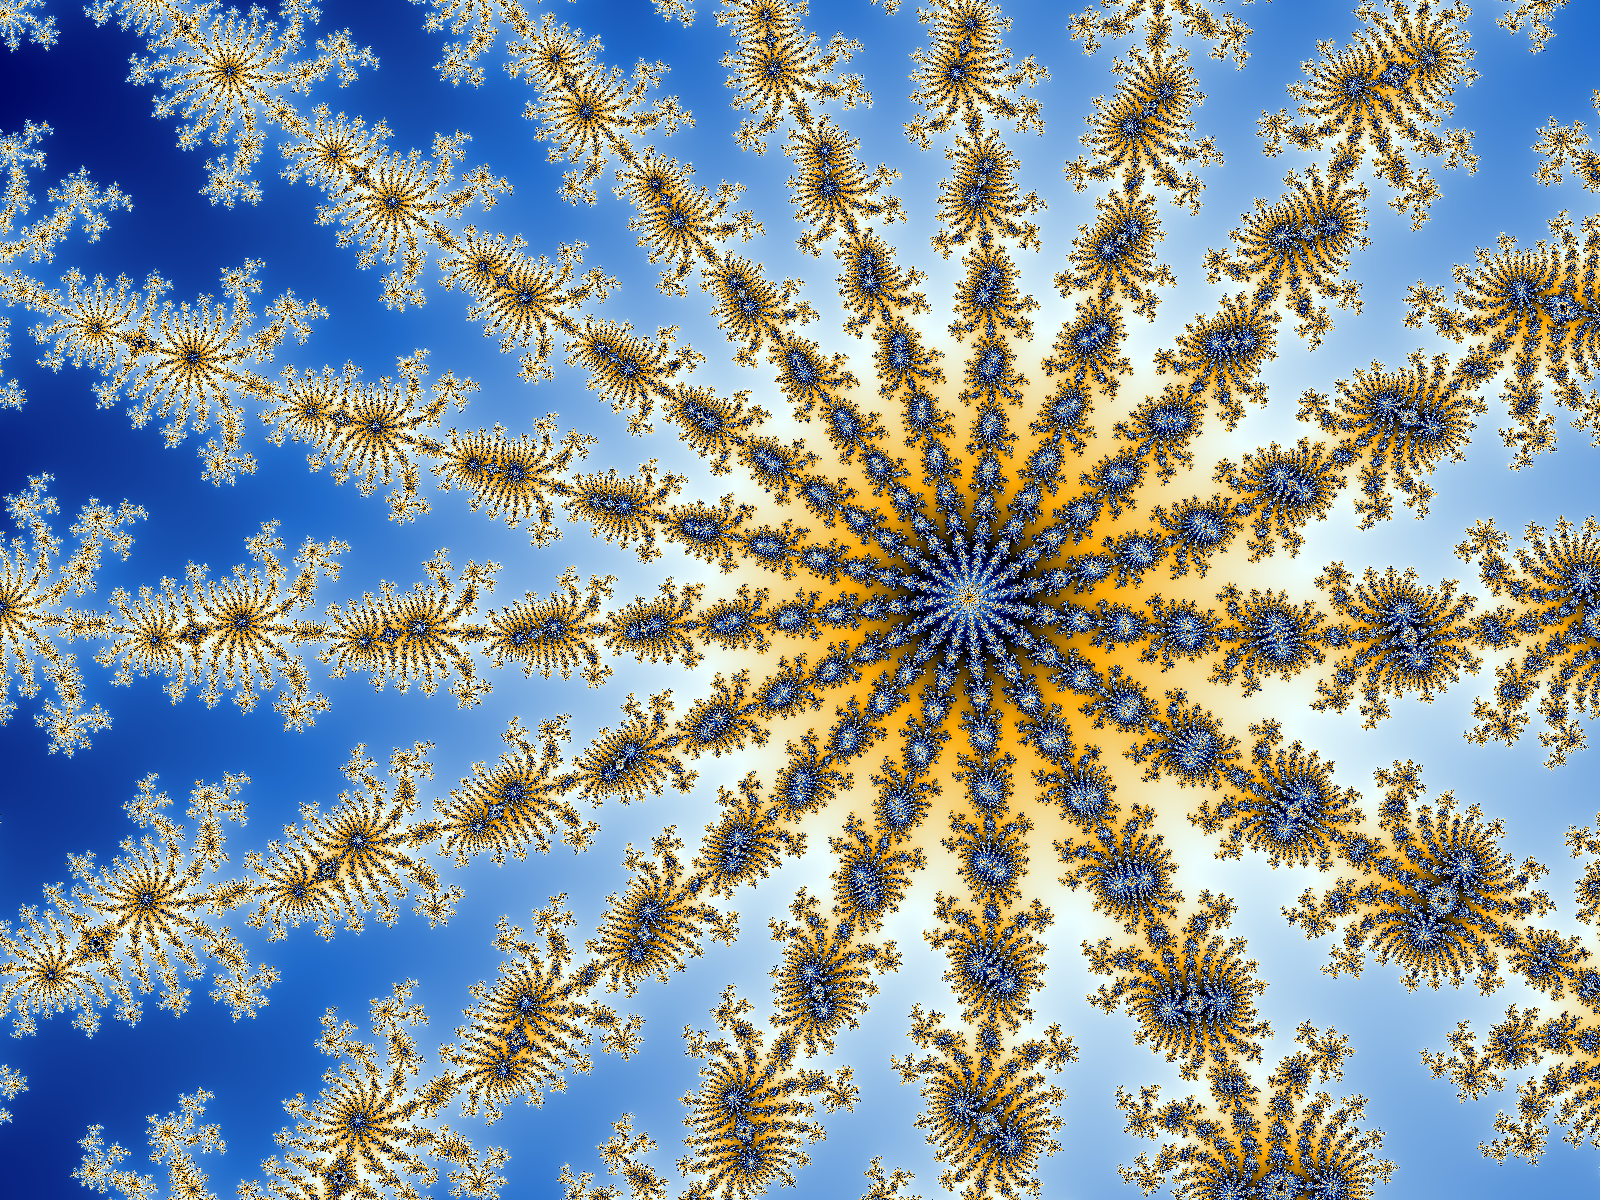
\includegraphics[width=1.1\textwidth]{data/mb4.png}}
\centerline{stred $(-0.65550685,0.3783525)$ }
\centerline{$m=236.2$}
\ep

\begin{uloha}
  Pohraj sa s Mandelbrotovou množinou.
\end{uloha}

\fi

%%%%%%%%%%%%%%%%%%%%%%%%%%%%%%%%%%%%%%%%%%%%%%%%%%%%%%%%%%%%%%%%%%%%%%%%%%%%
\if\sectxxv1
\section{vyhľadávacie stromy: {\tt<set>} a {\tt<map>} v STL}

Pri farbení Mandelbrotovej množiny v závere minulej kapitoly som robil túto vec:
''{\em \ldots pre každý počet iterácií } [som] {\em našiel maximálnu a minimálnu hodnotu
\ldots}''. Ak si sa pozrel do môjho programu, tak si videl, že som trochu cheatoval
a použil som typ \prg!map! z STL, o ktorom som ti doteraz nehovoril. Ale v tejto
kapitole to chcem napraviť. Začnime jednoduchou rozcvičkou:

\begin{uloha}
  Na vstupe je číslo $n$. A potom postupnosť príkazov. Každý príkaz je tvaru
  {\tt ! x} alebo {\tt ? x} a posledný príkaz je {\tt \#}. 
  Predpokladajme, že máme $n$ žiaroviek očíslovaných $1,\ldots,n$, 
  ktoré su na začiatku vypnuté. Príkaz {\tt ! x} znamená, že sme prepli žiarovku
  číslo $x$ (ak bola vypnutá, bude zapnutá a naopak). Pre každý príkaz {\tt ? x}
  treba vypísať, {\tt svieti} alebo {\tt nesvieti} podľa toho, v akom stave je práve žiarovka
  číslo $x$.
\end{uloha}

Jednou z možností, ako túto úlohu vyriešiť, bolo urobiť si vektor $n$ hodnôt typu \prg!bool!,
napr. \prg!vector<bool> a(n,false)! tak, že v \prg!a[i]! si budeme udržiavať stav $i$-tej
žiarovky. Predpokladajme teraz ale, že by žiarovky neboli očíslované $1$ až $n$, ale
že by mali iba výrobné čísla. Vstup by mohol vyzerať napríklad:
\begin{verbatim}
! 3736272
! 843984
? 3736272
! 84872634
! 72876
? 99
? 843984
#
\end{verbatim}

Problém je, že nevieme, aké výrobné čísla sa na vstupe objavia. Nemôžme si držať v pamäti 
pole pre všetky možné čísla, takže chceme mať zapamätané iba tie žiarovky, ktoré sme 
už videli. Teraz ale stoja proti sebe dve veci: ak chcem nájsť stav žiarovky s číslom 
{\tt id}, hodilo by sa mi mať žiarovky utriedené podľa čísla: mohol by som použiť
binárne vyhľadávanie, aby som zistil, či {\tt id} svieti. Ak ich utriedené nemám,
musím zakaždým prejsť všetky, čo trvá dlho. Na druhej strane, keď sa  objaví nová
žiarovka, ľahko ju pridám na koniec, ale potom nebudú utriedené. Musel by som 
všetky žiarovky v poli poposúvať, čo zase trvá dlho. 
Riešenie je namiesto poľa (vektora) použiť dátovú štruktúru, ktorá nemá všetky dáta
v jednom kuse pamäte, ale vo viacerých, ktoré na seba navzájom ukazujú pointrami. Tým
sa bude dať docieliť, že pri vkladaní mového prvku
bude namiesto posúvania všetkých hodnôt stačiť presmerovať
zopár pointrov. 

\ods Aby som ti ukázal, ako také štruktúry fungujú, začnime s jednoduchším príkladom
a k žiarovkám sa vrátime na konci kapitoly.

\begin{uloha}
  Úradník má kartotéku, kde má uložené spisy očíslované $0,1,\ldots,n-1$ (na začiatku
  v tomto poradí).
  Keď potrebuje nájsť spis $i$, začne prehľadávať zaradom od začiatku kartotéky
  a vždy prečíta číslo spisu, až kým nenájde ten s číslom $i$. Ten potom použije a 
  uloží na začiatok kartotéky. Napíš program, ktorý má na vstupe čísla $n, m$ a potom
  $m$ čísel spisov (medzi 0 a $n-1$). Pre každé číslo spisu vypíš riadok, v ktorom 
  sú čísla spisov, ktoré úradník prečítal pri hľadaní. Napríklad

  \ods
  \bp
  \begin{verbatim}
6 4
5
3
4
1
\end{verbatim}
\ep
\bp
\begin{verbatim}
0 1 2 3 4 nasiel som 5!
5 0 1 2 nasiel som 3!
3 5 0 1 2 nasiel som 4!
4 3 5 0 nasiel som 1!
\end{verbatim}
\ep
\end{uloha}

Na riešenie použijeme dátovú štruktúru {\em spájaný zoznam} ({\em linked list}).
Každý prvok zoznamu je uložený v samostatne alokovanej pamäti a má pointer
na nasledujúci prvok. Spravíme si typ

\begin{lstlisting}
struct Node {
  int val;
  Node *nxt;
  Node(int _val = -1, Node *_nxt = nullptr) {
    val = _val;
    nxt = _nxt;
  }
};
\end{lstlisting}

v ktorom bude jeden prvok zoznamu\footnote{%
  Možno ťa zaskočilo, že súčasťou typu {\tt Node} je premenná {\tt nxt}, ktorá
  je pointer na typ {\tt Node}. Nie je v tom ale nič zvláštne -- pointer je iba číslo
  adresy v pamäti. Typ pointra (v našom prípade {\tt Node *}) iba hovorí kompilátoru,
  že na adrese uloženej v premennej {\tt nxt} má očakávať premennú typu {\tt Node}.
  Pretože všetky pointre sú rovnako dlhé, kompilátoru nevadí, že typ {\tt Node} zatiaľ nie 
  je pripravený, stačí mu vedieť, koľko miesta treba v pamäti vyhradzovať.
  }. V programe budeme mať zoznam zapamätaný iba pointrom
na jeho začiatok \prg!Node *head;! Zoznam {\tt [0 1 2 3 4 5]} by v pamäti vyzeral takto:
    

    \def\llnode(#1,#2)[#3]#4{
      \begin{scope}[shift={(#1,#2)}]
        \draw [\nodecolor, rounded corners=2pt] (-0.5,-0.5) rectangle (0.5,0.5)
        (-0.5,0) -- (0.5,0)
        (-0.5,0.25) node [anchor=west]{{\tt val:}}
        (0.3,0.25) node[anchor=center]{{\tt #4}}
        (-0.5,-0.25) node [anchor=west]{{\tt nxt:}}
        (0.3,-0.25) node[anchor=center] {$\bullet$};
        \coordinate (n#3) at (0.3,-0.25);
        \coordinate (b#3) at (-0.5,0.25);
      \end{scope}
    }

    \def\head(#1,#2){
      \node[\nodecolor,anchor=east] (head) at (#1,#2) {{\tt head:}};
      \node[\nodecolor,right = 0mm of head, ] (headbullet) {$\bullet$};
    }

\ods
\centerline{
  \begin{tikzpicture}[xscale=1.4*0.8,yscale=0.8]
    {\small
    \def\nodecolor{cyan!50!blue}
    \foreach \v/\c[count =\i] in {0/A, 1/B, 2/C, 3/D, 4/E, 5/F} {
      \llnode(1.5*\i,0.5)[\c]{\v}
    }
    \foreach \x/\y in {A/B, B/C, C/D, D/E, E/F} {
    \draw[->,\nodecolor,shorten >= 0.15ex](n\x) to[out=0, in=180] (b\y);
    }
    \head(0,0);
    \draw[\nodecolor,->, shorten >= 0.15ex] (headbullet) to[out=0,in=180] (bA);
    \draw[\nodecolor,-|] (nF) to [out=0,in=90] ++(0.5,-0.5);
    }
  \end{tikzpicture}
}

\ods
Vyrobíme ho jednoducho:

\begin{lstlisting}
head = nullptr;
for (int i = 0; i < n; i++)
  head = new Node(n - 1 - i, head);
\end{lstlisting}

V cykle vždy pri vyhodnocovaní pravej strany priradenia 
vyrobíme novú premennú typu {\tt Node}, v ktorej nastavíme {\tt val}
na správnu hodnotu a {\tt nxt} na rovnaké miesto, ako v práve ukazuje {\tt head}.
V priradení potom nastavíme {\tt head}, aby ukazoval na túto novú premennú.

\ods
\centerline{

  \begin{tikzpicture}[xscale=1.4*0.8, yscale=0.8]
    {\small
    \def\nodecolor{cyan!50!blue}
    \foreach \v/\c[count =\i] in {4/A, 5/B} {
      \llnode(0.8+1.5*\i,0.5)[\c]{\v}
    }
    \foreach \x/\y in {A/B} {
    \draw[->,\nodecolor,shorten >= 0.15ex](n\x) to[out=0, in=180] (b\y);
    }
    \head(0,0);
    \draw[\nodecolor,->, shorten >= 0.15ex] (headbullet) to[out=0,in=180] (bA);
    \draw[\nodecolor,-|] (nB) to [out=0,in=90] ++(0.5,-0.5);
    
    \def\nodecolor{orange!80!black}
    \llnode(0.5,1.2)[C]{3}
    \draw[\nodecolor,->, shorten >= 0.15ex] (nC) to [out=0,in=90] ($(bA)+(0.5,0.25)$);
    }  
  \end{tikzpicture}
  \hfill
  \begin{tikzpicture}[xscale=1.4*0.8,yscale=0.8]
    {\small
    \def\nodecolor{cyan!50!blue}
    \foreach \v/\c[count =\i] in {4/A, 5/B} {
      \llnode(1.5+1.5*\i,0.5)[\c]{\v}
    }
    \foreach \x/\y in {A/B} {
    \draw[->,\nodecolor,shorten >= 0.15ex](n\x) to[out=0, in=180] (b\y);
    }
    \head(0,0);
    
    \llnode(1.5,1.2)[C]{3}
    \draw[\nodecolor,->, shorten >= 0.15ex] (nC) to [out=0,in=90] ($(bA)+(0.5,0.25)$);
    
    \draw[\nodecolor,-|] (nB) to [out=0,in=90] ++(0.5,-0.5);
    
    \def\nodecolor{orange!80!black}
    \draw[\nodecolor,->, shorten >= 0.15ex] (headbullet) to[out=0,in=180] (bC);
   }
  \end{tikzpicture}
}

\ods
Povedzme, že už máme vyrobený zoznam a máme v ňom nájsť hodnotu {\tt x}\footnote{%
a sme si istí, že {\tt x} sa v zozname nachádza, takže nemusíme kontrolovať, či sme
prišli na koniec zoznamu}. Spravím si premennú {\tt Node *p = heaad;}, s ktorou pôjdem
po zozname

\begin{lstlisting}
while (p->val != x) p = p->nxt;
\end{lstlisting}

Teraz budem v situácii, že {\tt p} ukazuje na hľadaný prvok:

\ods
\centerline{
  \begin{tikzpicture}[xscale=1.4*0.8,yscale=0.8]
    {\small
    \def\nodecolor{cyan!50!blue}
    \foreach \v/\c[count =\i] in {0/A, 1/B, 2/C, 3/D, 4/E, 5/F} {
      \llnode(1.5*\i,0.5)[\c]{\v}
    }
    \foreach \x/\y in {A/B, B/C, C/D, D/E, E/F} {
    \draw[->,\nodecolor,shorten >= 0.15ex](n\x) to[out=0, in=180] (b\y);
    }
    \head(0,0);
    \draw[\nodecolor,->, shorten >= 0.15ex] (headbullet) to[out=0,in=180] (bA);
    \draw[\nodecolor,-|] (nF) to [out=0,in=90] ++(0.5,-0.5);
    
    \def\nodecolor{orange!80!black}
    \draw[\nodecolor,->, shorten >= 0.15ex ] (4*1.5,1.5) node[anchor=south]{{\tt p}} 
    -- ++(0,-0.5);
    }
  \end{tikzpicture}
}

\ods Ako presunúť nájdený prvok na začiatok zoznamu? Najprv ho vypojím a potom napojím
na začiatok. Na vypojenie potrebujem nastaviť {\tt nxt} v predchodcovi na {\tt p->nxt}.
Preto si upravím cyklus, ktorým prechádzam zoznam tak, aby som našiel aj predchodcu {\tt p}:

\begin{lstlisting}
Node *p = head, *prev = nullptr;
while (p->val != x) {
  prev = p;
  p = p->nxt;
}
if (prev != nullptr) 
  prev->nxt = p->nxt;
\end{lstlisting}

\ods
\centerline{
  \begin{tikzpicture}[xscale=1.4*0.8,yscale=0.8]
    {\small
    \def\nodecolor{cyan!50!blue}
    \foreach \v/\c[count =\i] in {0/A, 1/B, 2/C, 3/D, 4/E, 5/F} {
      \llnode(1.5*\i,0.5)[\c]{\v}
    }
    \foreach \x/\y in {A/B, B/C, D/E, E/F} {
    \draw[->,\nodecolor,shorten >= 0.15ex](n\x) to[out=0, in=180] (b\y);
    }
    \head(0,0);
    \draw[\nodecolor,->, shorten >= 0.15ex] (headbullet) to[out=0,in=180] (bA);
    \draw[\nodecolor,-|] (nF) to [out=0,in=90] ++(0.5,-0.5);
    
    \def\nodecolor{orange!80!black}
    \draw[\nodecolor,->, shorten >= 0.15ex ] (4*1.5,1.5) node[anchor=south]{{\tt p}} 
    -- ++(0,-0.5);
    
    \def\nodecolor{green!50!black}
    \draw[\nodecolor,->, shorten >= 0.15ex ] (3*1.5,1.5) node[anchor=south]{{\tt prev}} 
    -- ++(0,-0.5);
     
     \draw[\nodecolor,->, shorten <= 0.5ex, shorten >= 0.15ex ] (nC) to [out=-80,in=270]
     ($(bE)+(0.5,-0.75)$);
 

    }
  \end{tikzpicture}
}

\ods
Teraz môžem presunúť {\tt p} na začiatok podobne, ako pri vytváraní zoznamu:

\begin{lstlisting}
p->nxt = head;
head = p;
\end{lstlisting}

\ods Celé riešenie potom vyzerá takto:

\begin{lstlisting}
int main() {
  int n, m;
  cin >> n >> m;
  Node *head = nullptr;
  for (int i = 0; i < n; i++)
    head = new Node(n - 1 - i, head);
  while (m > 0) {
    m--;
    int x;
    cin >> x;
    Node *p = head, *prev = nullptr;
    while (p->val != x) {
      cout << p->val << " ";
      prev = p;
      p = p->nxt;
    }
    cout<<"nasiel som "<<x<<"!"<<endl;
    if (prev != nullptr) {
      prev->nxt = p->nxt;
      p->nxt = head;
      head = p;
    }
  }
}
\end{lstlisting}

\begin{uloha}
  Pri riešení úlohy~\ref{uloha:mergesort} (MergeSort) v kapitole~\ref{sect:binarysearch}
  sme v operácii {\em merge}
  vždy prechádzali dve polia a výsledok kopírovali do tretieho. Napíš program na 
  triedenie algoritmom {\em MergeSort}, ktorý používa spájané zoznamy (funkcia
  {\tt sort} dostane ako parameter začiatok zoznamu) a nekopíruje
  dáta.
\end{uloha}

\ods
Spájaný zoznam a pole sú v istom zmysle opakom jeden druhého: v poli sa dá jednoducho prejsť
na hociktorý prvok, ale zle sa preusporiadava, lebo prvky treba kopírovať. V spájanom zozname
sa zle prechádza na konkrétny prvok, lebo treba prejsť celý zoznam, ale dobre sa
preusporiadava, lebo stačí poprehadzovať pointre. Skúsme spojiť dobré vlastnosti z oboch.
Binárne vyhľadávanie v usporiadanom poli\footnote{%
  nateraz nás bude zaujímať pole, v ktorom sa hodnoty neopakujú -- 
  ako v príklade so žiarovkami} sa dá predstaviť ako rozhodovací strom:

\ods
\centerline{\begin{tikzpicture}[scale=0.8]
  \foreach \h[count=\i] in {1,2,1,3,1,2,1,4,1,2,1,3,1,2,1} {
    \draw[thin,gray,dotted] (\i+0.5,0.5) -- (\i+0.5,1.2+1.2*\h) coordinate (tmp-\i);
 
  }

  \foreach \i/\d  in {2/1,4/2,6/1,8/4,10/1,12/2,14/1} {
    \pgfmathtruncatemacro{\prev}{\i-\d}
    \pgfmathtruncatemacro{\next}{\i+\d}
    \draw[thick] (tmp-\prev) -- (tmp-\i) -- (tmp-\next);
  }

  \foreach \v [count=\i] in { 12,14,17,21,25,29,30,32,34,37, 38,41,42,45,49} {
    \filldraw[fill=yellow!20!white](\i,0) rectangle node[anchor=center]{{\tt \v}} (\i+1,1);

    \filldraw[fill=green!10!white] (tmp-\i) circle (2.2ex) node [anchor=center] {{\tt \v}};
  }
  
  \draw[thick,red] (11,0) rectangle (12,1);
  \foreach \i in {8,12,10,11} {
    \draw[very thick,red] (tmp-\i) circle(2.2ex);
  }

\end{tikzpicture}}

\ods
Keď chceme nájsť číslo $38$, najprv sa pozrieme do stredu, porovnáms číslon $32$, keďže
$38>32$, vydáme sa vpravo, porovnáme so $41$ atď. Našim cieľom teraz bude vyrobiť si takýto
rozhodovací strom v pamäti pomocou smerníkov. Keď sa pozrieš na obrázok, vidiš, že strom
sa skladá z krúžkov, ktoré budem volať {\em uzly} alebo {\em vrcholy}. V každom uzle 
je číslo, ktorému budem hovoriť {\em kľúč}. Najvyšší uzol v strede (na obrázku $32$) 
bude {\em koreň}, uzly naspodu budú {\em listy}. Z každého uzla okrem listu vedú 
dve čiary ({\em hrany}), ktoré vedú do koreňov menších stromov (tým hovoríme
{\em synovia} uzla). Najdlhšia vzdialenosť od koreňa do nejakého listu sa volá 
{\em hĺbka}. Základná vlastnosť,
ktorá umožňuje binárne vyhľadávanie, je to, že v celom strome aj vo všetkých podstromoch
platí: \cmd{keď si zoberiem hocijaký vrchol $v$, tak všetky kľúče v podstrome, ktorého koreň 
je ľavý syn $v$, sú menšie ako kľúč vo $v$
a všetky kľúče v podstrome, ktorého koreň je pravý syn $v$, sú zase väčšie}. 
Takýto strom budeme volať {\em binárny vyhľadávací strom}.
Spravme si takýto typ:

\begin{lstlisting}
struct Node {
  int key;
  Node *left, *right;

  Node(int _key = 0, Node *_l = nullptr, Node *_r = nullptr) {
    key = _key;
    left = _l;
    right = _r;
  }

  ~Node() {
    if (left != nullptr) delete left;
    if (right != nullptr) delete right;
  }

};
\end{lstlisting}

\ods
Vyzerá veľmi podobne ako pri spájanom zozname, len má dva pointre (na ľavého 
a pravého syna). 
Pridal som navyše deštruktor: ak sa ide z pamäti odstrániť
premenná typu {\tt Node} (či už pri volaní \prg!delete! alebo inak), najprv sa
zavolá deštruktor, ktorý sa pozrie, že existuje ľavý a/alebo pravý syn a ak áno,
rekurzívne ich zmaže (t.j. zavolá sa deštruktor ľavého syna, ktorý zavolá deštruktor
jeho synov atď), až sa zmaže celý strom. 

\ods
Ak máme utriedené pole prvkov, môžeme z neho vyrobiť strom napríklad takto:

\vbox{
  \begin{lstlisting}
Node *vyrob(vector<int> &a, int i, int j) {
  Node *res = new Node();
  if (i == j) {
    res->key = a[i];
  } else {
    int m = (i + j) / 2;
    res->key = a[m];
    if (i != m) res->left = vyrob(a, i, m - 1);
    if (m != j) res->right = vyrob(a, m + 1, j);
  }
  return res;
}
  \end{lstlisting}
}

\ods
Funkcia {\tt vyrob} má ako parametre referenciu na vektor a dva indexy {\tt i}
a {\tt j} a vyrobí strom, ktorý bude mať kľúče z úseku \prg!a[i]!\ldots\prg!a[j]!
(vrátane): zistí sa stredný prvok {\tt a[m]} a ak je ľavý alebo pravý úsek neprázdny,
rekurzívne sa zavolá {\tt vyrob} a novovytvorené podstromy sa priradia do pointrov
{\tt left} a {\tt right}. Ak mám napr. pole {\tt [10, 11, 14, 16, 20, 32, 42, 47, 50]}
a zvolám \prg!Node *root = vyrob(a, 0, a.size()-1);!, vyrobí sa v pamäti
takáto štruktúra z pointrov:

    \def\tnode(#1)[#2]#3{
      \begin{scope}[shift={(#1)}, xscale=1.3*0.7, yscale=0.7]
        \filldraw [\nodecolor, rounded corners=3pt, fill=white ] 
        (-0.5,-0.5) rectangle (0.5,0.5)
        (-0.5,0) -- (0.5,0)
        (0,0) -- (0,-0.5)
        (0,0.25) node [anchor=center]{\textcolor{magenta}{\tt #3}}
        (-0.25,-0.25) node[anchor=center] {\scriptsize {$\bullet$}}
        (0.25,-0.25) node[anchor=center] {{\scriptsize $\bullet$}}
        ;
        \coordinate (#2l) at (-0.25,-0.25);
        \coordinate (#2r) at (0.25,-0.25);
        \coordinate (#2) at (0,0.5);
        \coordinate (#2h) at (-0.5,0);
      \end{scope}
    }

\ods
\centerline{
  \begin{tikzpicture}[scale=0.8]
    {\small
    \def\nodecolor{cyan!50!blue}
    \foreach \h[count=\i] in {1,2,1,3,1,2,1,4,1,2,1,3,1,2,1} {
      \coordinate (tmp-\i) at (0.9*\i,0.15*\h*\h+0.8*\h) ;
    }

    \foreach \v/\c[count=\i] in {10/2, 11/4, 14/6, 16/7, 20/8, 32/10, 42/12, 47/14, 50/15} {
      \tnode(tmp-\c)[n\i]{\v}
    }

    
    \foreach \a/\b in {n2l/n1,n2r/n3,n3r/n4,n5l/n2,n5r/n7,n7l/n6,n7r/n8,n8r/n9} {
      \draw[\nodecolor,->,shorten >= 0.2ex] (\a) to[out=270,in=90] (\b);
    }
    \draw[\nodecolor,->,shorten >= 0.2ex, shorten <= 0.5ex ] ($(n5)+(0,0.5)$)
    node[anchor=south]{{\tt root}} -- (n5);
    }
  \end{tikzpicture}
}


\ods
Keď chceme zistiť, či sa nejaký kľúč v strome nachádza, stačí prechádzať stromom 
od koreňa (napr. \prg!root->find(42);!). 
Metóda {\tt find} vráti pointer na uzol s daným kľúčom,
alebo \prg!nullptr!, ak sa tam kľúč nenachádza. 

\begin{lstlisting}
struct Node {
  int key;
  Node *left, *right;
  Node(int _key = 0, Node *_l = nullptr, Node *_r = nullptr) {...}
  ~Node() {...}

  Node *find(int x) {
    if (x == key) return this;
    if (x < key && left != nullptr) return left->find(x);
    if (x > key && right != nullptr) return right->find(x);
    return nullptr;
  }
};
\end{lstlisting}

\ods
Teraz sme docielili, že v pamäti máme namiesto poľa prvky pospájané smerníkmi
a môžeme v nich vyhľadávať rovnako, ako pri binárnom vyhľadávaní v poli (teda
v logaritmickej zložitosti). Pomohli ale v tom, že aj pridanie prvku má logaritmickú
zložitosť: jednoducho ideme po strome, ako keby sme vyhľadávali, a keď prídeme
na koniec, vyrobíme nový uzol. Metóoda {\tt insert} vráti \prg!true!, ak sa vrchol
v skutočnosti pridal a \prg!false!, ak už v strome bol:

\begin{lstlisting}
struct Node {
  int key;
  Node *left, *right;
  Node(int _key = 0, Node *_l = nullptr, Node *_r = nullptr) {...}
  ~Node() {...}
  Node *find(int x) {...}

  bool insert(int x) {
    if (x == key) return false;
    if (x < key && left != nullptr) return left->insert(x);
    if (x > key && right != nullptr) return right->insert(x);
    Node *nd = new Node(x);
    if (x < key) left = nd;
    else right = nd;
    return true;
  }

};
\end{lstlisting}

\ods
Zdá sa, že všetko funguje, a to je podozrivé. A naozaj. Keď začneš s jednoprvkovým
poľom {\tt [10]} a postupne voláš {\tt insert} pre $11, 14, 16, 20, 32, 42, 47, 50$,
v pamäti to bude vyzerať takto:

\ods
\centerline{
  \begin{tikzpicture}[scale=0.8]
    {\small
    \def\nodecolor{cyan!50!blue}

    \foreach \v[count=\i] in {10, 11, 14, 16, 20, 32, 42, 47, 50} {
      \tnode(\i,0-\i)[n\i]{\v}
    }

    
    \foreach \i in {1,...,8} {
      \pgfmathtruncatemacro{\j}{\i+1}
      \draw[\nodecolor,->,shorten >= 0.2ex] (n\i r) to[out=270,in=90] (n\j);
    }
    \draw[\nodecolor,->,shorten >= 0.2ex, shorten <= 0.5ex ] ($(n1)+(0,0.5)$)
    node[anchor=south]{{\tt root}} -- (n1);
    }
  \end{tikzpicture}
}

\ods
Takže mám obyčajný spájaný zoznam a vyhľadávanie je má lineárnu zložitosť.
Problém je, samozrejme, v tom, že pridanie prvku môže spôsobiť, že strom 
prestane byť {\em vyvážený}, t.j. prestane platiť, že v každom uzle je hĺbka
ľavého a pravého podstromu skoro rovnaká. Tomu sa dá zabrániť tak, že po 
každom vložení prvku sa zavolá {\em vyvažovacia operácia}, ktorá zabezpečí, 
že strom bude ''rozumne''\footnote{%
t.j. tak, aby bolo zaručené, že operácie majú logaritmickú zložitosť}
vyvážený. Je veľa spôsobov, ako toto vyvažovanie urobiť (AVL stromy, Red-Black stromy,
\ldots). Ukážem ti jeden spôsob, zvaný AA stromy. 

\ods
Celý prístup vyzerá takto: najprv si poviem pravidlá, ktoré musí AA strom spĺňať. Potom
sa presvedčím, že každý strom, ktorý tieto pravidlá spĺňa, má logaritmickú hĺbku. Nakoniec
naprogramujem operácie (vkladanie, vyhľadávanie, mazanie) tak, aby udržovali splnené pravidlá
a navyše ich zložitosť bola úmerná hĺbke. Tak poďme na to.

\ods
V AA-strome má každý uzol okrem kľúča aj ''poschodie'' ({\em level}). Pre zjednodušenie
použijeme techniku zarážky a vyrobíme jeden špeciálny uzol {\em ''prízemie''}, ktorý bude na 
leveli 0. Pravidlá pre dobrý AA-strom sú takéto:

\ods

\centerline{\fcolorbox{magenta}{magenta!3!white}{\parbox{0.9\textwidth}{
\begin{enumerate}\itemsep=-1mm
\item Je to binárny vyhľadávací strom: v každom uzle platí, že všetky uzly v ľavom podstrome
  majú menšie kľúče a všetky uzly v pravom podstrome väčšie.
\item Každý uzol (okrem prízemia) má dvoch synov. 
\item \label{aarule3} Ľavý syn je na leveli o 1 menšom ako rodič.
\item Pravý syn je na rovnakom alebo o 1 menšom leveli ako rodič.
\item \label{aarule5} 
  Ak je pravý syn na rovnakom leveli ako rodič, jeho pravý syn je na menšom leveli.
\end{enumerate}
}}}

\ods Pravidlo~\ref{aarule5} hovorí, že nemôžu byť na rovnakom leveli tri uzly
rodič -- pravý syn -- jeho pravý syn. Zároveň, keďže prízemie má level 0, tak
podľa pravidla~\ref{aarule3}, listy musia byť na leveli 1 atď. AA-strom teda vyzerá nejak 
takto (farebné pásy sú levely):


\def\level(#1:#2)[#3]#4 {
  \fill[fill=#3] (\levelmin,#1) rectangle (\levelmax,#2);
}

\ods
\centerline{
  \begin{tikzpicture}[
      nodelink/.style={#1, ->, shorten >= 0.2ex},
      nodelink/.default={cyan!50!blue},
      scale=0.8]
    {\small

    \def\levelmin{-0.7}
    \def\levelmax{18.2}
    \level(-1:0.9)[green!10!white]{}
    \level(0.9:2.7)[yellow!10!white]{}
    \level(2.7:4.5)[orange!10!white]{}
    \level(4.5:6.4)[red!10!white]{}

    \def\nodecolor{cyan!50!blue}
    \foreach \x/\y/\v[count=\i] in {
      0/0.1/1,1/-0.1/2,2/0.1/4,3/-0.1/5,4/0.1/7,5/0.1/9,6/0.1/11, 7/0.1/13,8/0.1/15,
    9/0.1/17,10/0.1/19,11/-0.1/20,12/0.1/22,13/-0.1/23,14/0.1/25,
    1.5/1.1/3, 3/0.9/6, 5.5/1/10, 7.5/1.1/14, 8.5/0.9/16, 11.5/1.1/21, 12.55/0.9/24,
    4.5/2.12/8,9.5/2.12/18, 7.5/3.25/12
    } {
      \tnode(1.25*\x,1.8*\y)[n\i]{\v}
    }

    \coordinate (base) at (8.75,-1.7);
    \foreach \i/\d in {1/l,2/l,2/r,3/l,4/l,4/r,5/l,5/r,6/l,6/r,7/l,7/r,8/l,8/r,9/l,9/r,10/l,
    10/r,11/l,12/l,12/r,13/l,14/l,14/r,15/l,15/r} 
      \draw[gray,very thin] (n\i\d) 
      .. controls ($ (n\i\d) + (0,-1.3) $) ..
    (base);
  

    \foreach \a/\b in {16l/1,17l/3,17r/5,18l/6,18r/7, 19l/8,20l/9,20r/10,21l/11,22l/13,22r/15,
    23l/16,23r/18,24l/19,24r/21,25l/23,25r/24}
    \draw[nodelink=\nodecolor](n\a) to [out=270,in=90](n\b);

    \foreach \a/\b in {1/2, 3/4,11/12,13/14,16/17,19/20,21/22}
    \draw[nodelink=\nodecolor](n\a r) to [out=0,in=180](n\b h);

    \def\nodecolor{gray}
    \tnode(base)[tmp]{  }

    }
  \end{tikzpicture}
}


\ods
Terz chcem vyrátať, akú najväčšiu hĺbku môže mať AA strom, v ktorom je $n$ uzlov. Spomeň si,
že hĺbka je dĺžka najdlhšej cesty z koreňa do nejakého listu. Keď začnem z koreňa a postupujem
smerom k listu, tak nikdy nejdem na vyšší level: buď idem na nižší (napr. z $18$ do
$14$) alebo ostávam na tom istom (napr. zo $14$ do $16$). Ale takitsto nemôžem ísť
cez viac ako dva uzly na jednom leveli. Takže hĺbka je najviac dvojnásobok počtu levelov.
Dobre. Poďme teda vyrátať, koľko najviac levelov môže mať AA-strom, ktorý má $n$ uzlov. 
Najprv sa opýtam tak trochu opačnú otázku: 
koľko najmenej listov môže mať AA-strom, ktorý má $\ell$ levelov?
Koreň je na najvyššom leveli (teda na leveli $\ell$). 
Jeho ľavý syn je koreň AA-stromu s $\ell-1$ levelmi. Ak je
pravý syn koreňa na nižšom leveli, tak je tiež
koreňom nejakého (iného) AA-stromu s $\ell-1$ levelmi.
Ak je pravý syn koreňa na rovnakom leveli (na leveli $\ell$), tak jeho ľavý syn je koreň 
AA-stromu s $\ell-1$ levelmi. V každom prípade, v AA-strome s $\ell$ levelmi
viem nájsť dva rôzne AA-stromy
s $\ell-1$ levelmi. Preto ak si označím $L(\ell)$ najmenší počet listov, ktorý môže
mať AA-strom s $\ell$ levelmi, tak $L(\ell)\ge2L(\ell-1)$.
Dostávam teda $L(1)=1$, $L(2)\ge2$, $L(3)\ge4$, $L(4)\ge8$, \ldots, t.j. 
$L(\ell)\ge2^{\ell-1}$. Teda AA-strom s $\ell$ levelmi musí mať aspoň $2^{\ell-1}$
uzlov. Vráťme sa teraz k pôvodnej otázke: koľko najviac levelov má AA-strom s $n$ uzlami?
Keby ich mal aspoň $2+\log n$, tak by musel mať 
$L(2+\log n)\ge2^{2+\log n-1}=2n$ listov. To ale nemôže, lebo má len $n$ uzlov. Takže
AA-strom s $n$ uzlami musí mať menej ako $2+\log n$ levelov, a preto má aj logaritmickú hĺbku.

\ods
Ostáva už len posledné: naprogramovať vkladanie, vyberanie a vyhľadávanie do AA-stromu tak,
aby ich zložitosť zodpovedala hĺbke stromu. Keďže AA-strom je binárny vyhľadávací strom,
vyhľadávanie je ľahké. Najprv si spravím typ \prg!Node! podobne ako predtým. Rozdiel
bude v tom, že uzol si navyše bude pamätať svoj level. Konštruktor aj metóda
\prg!find! okrem kľúča dostanú aj pointer na prízemie (\prg!base!).
Namiesto deštruktora budem mať procedúru \prg!destroy!, lebo deštruktory nemôžu
mať parametre a ja potrebujem vedieť, čo je zarážka.

\ods
\begin{lstlisting}
struct Node {
  int level, key;
  Node *left, *right;

  Node(int k, Node *base) { level = 1; key = k; left = right = base; }

  void destroy(Node *base) {
    if (this == base) return;
    left->destroy(base);
    right->destroy(base);
    delete this;
  }

  bool find(int k, Node *base) {
    if (this == base) return false;
    if (key == k) return true;
    if (k < key)
      return left->find(k, base);
    else
      return right->find(k, base);
  }
};
\end{lstlisting}

Urobím si aj nový typ \prg!Tree! pre celý strom, v ktorom budem mať zapamätaný koreň
a prízemie:

\ods
\begin{lstlisting}
struct Tree {
  Node *root, *base;

  Tree() {
    base = new Node(0,nullptr); // vyrobim si prizemie
    base->level = 0;
    base->left = base->right = base;
    root = base; 
  }

  ~Tree() { root->destroy(base); delete base; }

  bool find(int key) { return root->find(key, base); }
};
\end{lstlisting}

\ods
Pridávanie ale začne byť trochu komplikovanejšie. Zoberme si jednoduchú funckiu {\tt insert}
z predchádzajúceho prípadu. Začnem s prázdnym stromom a pridám doňho čísla $9$ a $20$. Bude to vyzerať nejak takto (modré číslo znamená level, čiarkovaná čiara je prízemie):

\def\aaangle{17}
\def\aanormalcolor{yellow!7!white}
\def\aanode(#1)#2#3{%
  \filldraw[thick, fill=\aanormalcolor] (#1) node {{\tt #2}} circle (2.2ex) 
        ++ (1ex,1ex) node [anchor=south west] {\textcolor{blue}{{\small\tt #3}}} ;
  }
\def\aasub(#1)#2#3{%
  \coordinate(tmp1) at ($(#1)+(270-16:1.3)$);
  \coordinate(tmp2) at ($(#1)+(270+16:1.3)$);
  \filldraw[thick, fill=green!7!white] 
      (#1) -- (tmp1) -- (tmp2) -- (#1);
  \def\tmpr{1.8ex}    
  \filldraw[thick, fill=green!7!white] 
      ($(#1)+(-\tmpr,-\tmpr)$) rectangle 
      node[align=center] {{\tt #2}} 
      ($(#1)+(\tmpr,\tmpr)$) 
      ($(#1)+ (\tmpr,\tmpr)$) node[anchor=south west]  {\textcolor{blue}{{\small\tt #3}}} ;
  }
\def\ground(#1)#2{
  \coordinate (tmp1) at ($(#1)+(270#2\aaangle:5)$);
  \coordinate (tmp2) at (intersection of #1--tmp1 and {-10,0}--{10,0});
  \draw(#1)--(tmp2);
}
\ods\centerline{
  \begin{tikzpicture}
    \foreach\x/\y[count=\i]in{0/1,1/0.87} 
      \coordinate (n\i) at (1.5*\x,1.5*\y);
  
    \draw[dashed](-1,0)--(2.5,0);
    \ground(n1)-
    \ground(n2)-
    \ground(n2)+
    \draw(n1)--(n2);
    \draw (n1) -- +(0,0.7);
    \aanode(n1){9}{1}
    \aanode(n2){20}{1}
  \end{tikzpicture}
}

\ods
Keď chcem pridať číslo $15$, vznikne problém:

\ods\centerline{
  \begin{tikzpicture}
    \foreach\x/\y[count=\i]in{0/1.4,1.6/1.2,1/0.5} 
      \coordinate (n\i) at (\x,1.5*\y);

    \draw[dashed](-1.2,0)--(2.7,0);
    \ground(n1)-
    \ground(n2)+
    \ground(n3)-
    \ground(n3)+
    \draw(n1)--(n2) --(n3);
    \draw(n1) -- +(0,0.7);
    \aanode(n1){9}{1}
    \aanode(n2){20}{1}
    \aanode(n3){15}{1}
  \end{tikzpicture}
}

\ods
Uzol $15$ musí byť na leveli 1, lebo je to list, ale zároveň je ľavým synom uzla $20$, preto
$20$ musí mať level $2$. Lenže pravý syn $20$ky je prízemie (s levelom 0), preto
$20$ musí mať level $1$. Takže je zrejmé, že nestačí len aktualizovať levely, ale bude treba 
prerobiť aj celý strom. V tomto príklade môžem na uzol $20$ použiť operáciu {\em skew} 
({\em posun}), ktorá vyzerá takto:

\ods
\centerline{\begin{tikzpicture}
\foreach\x/\y[count=\i]in{0/0, 1.4/0, 0.7/1.35, 2.2/1.8, 3/0}
      \coordinate (n\i) at (\x,\y);
      
\draw (n1) -- (n3) -- (n2) (n3)--(n4)--(n5) (n4) -- ++(0,0.7);   
\aanode(n3){$x$}{k}
\aanode(n4){$y$}{k}
\aasub(n1){$A$}{k-1}
\aasub(n2){$B$}{k-1}
\aasub(n5){$C$}{k-1}

\node[draw, single arrow, minimum height=22mm, minimum width=8mm,
  single arrow head extend=2mm, anchor=center] at (5.5,0.7) {};

\begin{scope}[shift={(8,0)}]
  \foreach\x/\y[count=\i]in{0/0, 1.6/0, 0.7/1.8, 2.2/1.35, 3/0}
      \coordinate (n\i) at (\x,\y);
      
  \draw (n1) -- (n3) --(n4) (n2)--(n4)--(n5) (n3) -- ++(0,0.7);   
  \aanode(n3){$x$}{k}
  \aanode(n4){$y$}{k}
  \aasub(n1){$A$}{k-1}
  \aasub(n2){$B$}{k-1}
  \aasub(n5){$C$}{k-1}
\end{scope}

\end{tikzpicture}}


\ods
Povedané slovami: ak mám podstrom s koreňom $y$ na leveli $k$, 
ktorý má ľavého syna $x$ na leveli $k$ (čím
sa porušilo pravidlo~\ref{aarule3}) a $x$ má obidvoch synov na leveli $k-1$, môžem 
za koreň podstromu zvoliť $x$ a pravého syna $x$ prevesiť pod $y$. Po operácii posun
strom ostane dobrý vyhľadávací strom, lebo všetky kľúče v podstrome $B$ sú menšie ako $y$.
Operáciu \prg!skew! si naprogramujem ako metódu \prg!Node!. Zavolám ju v koreni
podstromu (napr. \prg!root=root->skew()!) a bude vracať
pointer na nový koreň stromu:

\begin{lstlisting}
Node *skew() {
  if (left->level != level) return this;
  Node *res = left, *tmp = left->right;
  left->right = this;
  left = tmp;
  return res;
}
\end{lstlisting}
\ods

Ak aplikujem {\tt skew} na uzol $20$ z príkladu, dostanem 

\ods\centerline{
  \begin{tikzpicture}
    \foreach\x/\y[count=\i]in{0/1.4,1.6/1.2,1/0.5} 
      \coordinate (n\i) at (\x,1.5*\y);

    \draw[dashed](-1.2,0)--(2.7,0);
    \ground(n1)-
    \ground(n2)+
    \ground(n3)-
    \ground(n3)+
    \draw(n1)--(n2) --(n3);
    \draw(n1) -- +(0,0.7);
    \aanode(n1){9}{1}
    \aanode(n2){20}{1}
    \aanode(n3){15}{1}

    \node[draw, single arrow, minimum height=20mm, minimum width=8mm,
  single arrow head extend=2mm, anchor=center] at (4.5,1) {};


    \begin{scope}[shift={(8,0)}]
    \foreach\x/\y[count=\i]in{0/1.3, 1.7/0.5, 1.2/1} 
      \coordinate (n\i) at (\x,1.5*\y);

    \draw[dashed](-1.2,0)--(2.7,0);
    \ground(n1)-
    \ground(n2)+
    \ground(n2)-
    \ground(n3)-
    \draw(n1)--(n3) --(n2);
    \draw(n1) -- +(0,0.7);
    \aanode(n1){9}{1}
    \aanode(n2){20}{1}
    \aanode(n3){15}{1}
    \end{scope}
  \end{tikzpicture}
}

\ods
Teraz som vyriešil problém v pravom podstrome uzla $9$, ale problém je v samotnej $9$ke:
uzly $15$ aj $20$ sú na leveli 1, a tým porušujú pravidlo~\ref{aarule5}. To ošetrím druhou
operáciou, ktorú nazvem {\em split} ({\em rozdelenie}) a vyzerá takto:

\ods
\centerline{\begin{tikzpicture}
\foreach\x/\y[count=\i]in{0.7/1.8,2.1/1.6,3.5/1.4, 0/0,1.4/0,2.8/0,4.2/0}
      \coordinate (n\i) at (\x,\y);
      
  \draw (n4) -- (n1) -- (n2) -- (n3)--(n7) (n5)--(n2) (n6)--(n3) (n1) -- ++(0,0.7);   
\aanode(n1){$x$}{k}
\aanode(n2){$y$}{k}
\aanode(n3){$z$}{k}
\aasub(n4){$A$}{k-1}
\aasub(n5){$B$}{k-1}
\aasub(n6){$C$}{k-1}
\aasub(n7){$D$}{k-1}

\node[draw, single arrow, minimum height=20mm, minimum width=8mm,
  single arrow head extend=2mm, anchor=center] at (6.5,0.7) {};

\begin{scope}[shift={(9,0)}]
\foreach\x/\y[count=\i]in{0.7/1.4,2.1/1.9,3.5/1.4, 0/0,1.4/0,2.8/0,4.2/0}
      \coordinate (n\i) at (\x,\y);
      
  \draw (n4) -- (n1) -- (n2) -- (n3)--(n7) (n5)--(n1) (n6)--(n3) (n2) -- ++(0,0.7);   
\aanode(n1){$x$}{k}
\aanode(n2){$y$}{k+1}
\aanode(n3){$z$}{k}
\aasub(n4){$A$}{k-1}
\aasub(n5){$B$}{k-1}
\aasub(n6){$C$}{k-1}
\aasub(n7){$D$}{k-1}
\end{scope}

\end{tikzpicture}}

\ods
Slovami, ak mám postupne dvoch pravých synov na rovnakom leveli ako rodič, môžem stredného
posunúť na vyšší level. Opäť to naprogramujem rovnako, ako predtým, t.j. ako metódu,
ktorá vracia pointer na nový koreň:

\ods
\begin{lstlisting}
 Node *split() {
    if (right->right->level != level) return this;
    right->level++;
    Node *res = right;
    right = right->left;
    res->left = this;
    return res;
  }
\end{lstlisting}
\ods
Keď aplikujem {\tt split} na vrchol $15$, výsledný strom bude

\ods\centerline{
  \begin{tikzpicture}
    \foreach\x/\y[count=\i]in{0/1.3, 1.7/0.5, 1.2/1} 
      \coordinate (n\i) at (\x,1.5*\y);

    \draw[dashed](-1.2,0)--(2.7,0);
    \ground(n1)-
    \ground(n2)+
    \ground(n2)-
    \ground(n3)-
    \draw(n1)--(n3) --(n2);
    \draw(n1) -- +(0,0.7);
    \aanode(n1){9}{1}
    \aanode(n2){20}{1}
    \aanode(n3){15}{1}

\node[draw, single arrow, minimum height=20mm, minimum width=8mm,
  single arrow head extend=2mm, anchor=center] at (4.5,1) {};

\begin{scope}[shift={(8,0)}]

    \foreach\x/\y[count=\i]in{0/0.5, 1.6/0.5, 0.8/1.4} 
      \coordinate (n\i) at (\x,1.5*\y);

    \draw[dashed](-1.2,0)--(2.7,0);
    \ground(n1)-
    \ground(n2)+
    \ground(n2)-
    \ground(n1)+
    \draw(n1)--(n3) --(n2);
    \draw(n3) -- +(0,0.7);
    \aanode(n1){9}{1}
    \aanode(n2){20}{1}
    \aanode(n3){15}{2}
\end{scope}
  \end{tikzpicture}
}

\ods
Pridaním listu a následným volaním {\tt skew} a {\tt split} sa mi mohlo stať, že
sa porušia pravidlá vyššie v strome. V mojom príklade je teraz koreň namiesto 
uzla $9$ s levelom $1$, uzol $15$ s levelom $2$. Keby to nebol celý strom, ale 
nad ním by bol napr. uzol $30$ s levelom $2$, porušilo by sa mi v ňom pravidlo~\ref{aarule3}.
Možnosti, ako sa to môže stať, sú ale rovnaké, ako pri pridávaní listu\footnote{%
  všimni si, že jediné miesto, kde level môže stúpnuť, je pri operácii {\tt split},
  ale potom sú obaja synovia na menšom leveli}. Preto celé pridávanie môžem napísať
  jednoducho takto:

\begin{lstlisting}
struct Node {
  int level, key;
  Node *left, *right;

  Node(int k, Node *base) { ... }
  void destroy(Node *base) { ... }
  bool find(int k, Node *base) { ... }
  
  Node *skew() { ... }
  Node *split() { ... }

  Node *insert(int k, Node *base) {
    if (this == base) return new Node(k, base);
    if (k == key) return this;
    if (k < key)
      left = left->insert(k, base);
    else
      right = right->insert(k, base);
    return skew()->split();
  }
};

struct Tree {
  Node *root;
  Node *base;

  Tree() { ... }
  ~Tree() { ... }

  void insert(int key) { root = root->insert(key, base); }
  bool find(int key) { return root->find(key, base); }
};

\end{lstlisting}

\ods
Uzly, ktoré sú v strome, sa dajú odstrániť podobným spôsobom. Ak mám odstrániť list,
nájdem ho ako pri vyhľadávaní, zmažem ho, a po zmazaní dovyvažujem strom. Problém je,
čo urobiť, ak mám vymazať uzol, ktorý nie je list. Pomôže drobná finta: ak mám
vymazať uzol $x$, ktorý má ľavého syna, nájdem si uzol $y$ s najväčším kľúčom v podstrome
ľavého syna (t.j. najpravejší list). Viem, že $y$ je väčší, ako všetky kľúče v ľavom podstrome
$x$ a zároveň menší, ako všetky kľúče v pravom podstrome. Môžem teda vymeniť hodnoty
$x$ a $y$, a už mi stačí vymazať list. Ak $x$ nemal ľavého syna, ale iba pravého, 
urobím to symetricky (hľadám najľavejší list). V súbore 
\link{\rootpath/aatree.h}{aatree.h}
je strom aj s dopísanou operáciou {\tt erase}: pri postupe smerom nadol
si v premennej {\tt deleted} uchovávam posledný uzol, ktorého kľúč je $\ge k$. Keď
prídem do príslušného listu (najľavejšieho alebo najpravejšieho), tak vymením
hodnoty a dovyvažujem strom (skús si premyslieť, ako to funguje).

\ods
Vráťme sa teraz k úlohe o žiarovkách s výrobnými číslami.
S použitím AA stromu je to ľahké.

\begin{uloha}
  Na vstupe je  postupnosť príkazov. Každý príkaz je tvaru
  {\tt ! x} alebo {\tt ? x} a posledný príkaz je {\tt \#}. 
  Predpokladajme, že máme žiarovky, 
  ktoré su na začiatku vypnuté. Príkaz {\tt ! x} znamená, že sme prepli žiarovku
  s výrobným číslom $x$ (ak bola vypnutá, bude zapnutá a naopak). Pre každý príkaz {\tt ? x}
  treba vypísať, {\tt svieti} alebo {\tt nesvieti} podľa toho, v akom stave je práve žiarovka
  číslo $x$.
\end{uloha}

Skús si napísať rekurzívnu funkciu na nasledujúcu úlohu:

\begin{uloha}
  Napíš funkciu, ktorá vypíše všetky kľúče z AA stromu v utriedenom poradí.
\end{uloha}


\ods
V STL sú podobné stromy naprogramované v type, ktorý sa volá {\em monžina} ({\em set}). 
Na pužitie treba pridať \prg!#include <set>!.
Je to šablóna, ktorá má ako parameter typ kľúča, takže napr. \prg!set<int> s;! je
strom, ktorý má 
kľúče typu \prg!int!. Namiesto \prg!int! to môže byť hocijaký iný typ, ktorý má definované
porovnanie. Pri vlastných typoch treba \prg!operator<! definovať ako \prg!const!,
napr. takto:

\begin{lstlisting}
struct Osoba {
  string meno, priezvisko;

  bool operator<(const Osoba& x) const {
    if (priezvisko == x.priezvisko) return meno < x.meno;
    return priezvisko < x.priezvisko;
  }
};
\end{lstlisting}

\prg!const! pri parametri {\tt x} 
znamená, že {\tt x} je referencia na premennú typu {\tt Osoba},
ale funkcia \prg!operator<! sľubuje, že {\tt x} nebude meniť. Podobne \prg!const! za menom
funkcie sľubuje, že sa nebude meniť \prg!*this!, t.j. ak zavolám \prg!x.operator<(y)!,
tak sa nezmení ani {\tt x} ani {\tt y}. 
Pri takejto definícii môžem použiť \prg!set<Osoba>! a budem mať v strome osoby utriedené podľa
priezviska a pri rovnakom priezvisku podľa mena.

\ods
Iná možnosť je použiť šablónu {\tt set}
s dvoma parametrami, kde druhý parameter je typ porovnávacej
funkcie, a porovnávacia funckia je potom parametrom konštruktora. 
Keby typ {\tt Osoba} nemal definované porovnanie, alebo keby som chcel
mať strom usporiadaný najprv podľa mena a potom podľa priezviska, môžem napísať
(potrebujem pridať \prg!#include <functional>!):

\begin{lstlisting}
set<Osoba, function<bool(const Osoba &, const Osoba &)>> s(
    [](const Osoba &x, const Osoba &y) {
      if (x.meno == y.meno) return x.priezvisko < y.priezvisko;
      return x.meno < y.meno;
    });
\end{lstlisting}

Tým hovorím, že chcem vyrobiť vyhľadávací strom s uzlami s hodnotou {\tt Osoba} a na 
porovnávanie budem používať funkciu (lambdu), ktorá zoberie referencie na dve premenné
typu {\tt Osoba} a vráti \prg!bool!.

\ods
Podobne ako v našom type {\tt Tree}, typ \prg!set! má
operácie \prg!s.insert(x)! a \prg!s.erase(x)!. Keďže je to kontainer, má 
definované aj iterátory\footnote{Na rozdiel od vektora, iterátor pre \prg!set! sa
dá posunúť len na susedný prvok, t.j. môžem mať \prg!it++! alebo \prg!it--!, ale 
nie \prg!it+10!}, takže napr.

\begin{lstlisting}
for (auto it = s.begin(); it != s.end(); it++) cout << *it << " ";
\end{lstlisting}

vypíše všetky prvky. Navyše je zaručené, že pri prechode iterátorom
budú prvky uspriadané od najmenšieho po najväčši. Vyhľadávanie prvku robí
metóda {\tt find(x)}, ktorá vráti iterátor na prvok s kľúčom {\tt x}, 
alebo {\tt end()}, ak tam 
prvok s daným kľúčom nie je.
Takže zistiť, či je kľúč {\tt x} v množine, sa dá pomocou \prg~if (s.find(x) != s.end())~
Metóda {\tt erase} má dve verzie: buď vymaže prvok s daným kľúčom alebo prvok s
daným iterátorom. Napr. \prg!s.erase(s.begin())! vymaže najmenší prvok.
Hodí sa ešte funkcia \prg!upper_bound(x)! (resp. \prg!lower_bound(x)!), ktorá vráti
iterátor na najmenší prvok väčší (resp. väčší alebo rovný) ako \prg|x|.

\ods
Ako presne je \prg!set! naprogramovaný je na konkrétnom kompilátore, ale musí zaručiť,
aby zložitosť všetkých operácií (vyhľadávanie, vkladanie, mazanie) bola logaritmická.
Existujúce kompilátory väčšinou používajú
tzv. {\em Red-Black} stromy, ktoré majú trochu iný spôsob vyvažovania, ale v podstate
sú veľmi podobné AA stromom. 
V nasledovnom grafe je porovnanie časov. Pre rôzne hodnoty $n$ som
povkladal do stromu $n$ rôznych čísel (v náhodnom poradí) a potom som ich (v náhodnom poradí)
zo stromu vymazal. Meral som si priemerný čas, ktorý trvala jedna operácia. Vidno, že
\prg!set! je trochu rýchlejší\footnote{a aj konzitentnejší, modrá krivka je viac roztrasená}, 
ako náš {\tt Tree}, ale zase nie až tak o veľa. V obidvoch
prípadoch rastie čas, ktorý treba na vloženie (vymazanie) iba veľmi pomaly 
v závislosti od veľkosti stromu.


\ods
\begin{tikzpicture}
\begin{axis}[
  width=\textwidth, 
  height=10cm,
  xlabel=$n$,
  ylabel=čas ($\mu$s),
  legend cell align={left},
  legend pos = north west,
  %  scaled x ticks=false,
  %scaled y ticks=false,
    /pgf/number format/.cd,
        1000 sep={}
]
  \addplot+[blue!80!white, 
  line join=round, mark size=0.5pt] table [y=aa, x=n]{data/tree_test.dat};
  \addlegendentry{{\tt aatree.h}}
  \addplot+[orange!80!white, 
  line join=round, mark size=0.5pt] table [y=set, x=n]{data/tree_test.dat};
  \addlegendentry{{\tt set<int>}}
\end{axis}
\end{tikzpicture}

\ods


\ods
V STL je aj niekoľko podobných dátových štruktúr. \prg!multiset! sa od \prg!set!
líši tým,
že dovoľuje mať viacero prvkov s rovnakým kľúčom\footnote{%
  Tu si treba dať pozor: \prg!s.erase(x)! vymaže všetky prvky s kľúčom \prg!x!.
  Na vymazanie jedného treba použiť \prg!s.erase(s.find(x))!, t.j. nájsť iterátor 
  na nejaký konkrétny uzol s kľúčom {\tt x} a potom vymazať ten.}. 

\ods
  Podobný ako \prg!set! je aj typ \prg!map!, v ktorom každý uzol 
  má okrem kľúča aj hodnotu. Je to šablóna s dvoma parametrami, 
  napr. \prg!map<string,int> m;! používa ako kľúč
  \prg!string! \footnote{\prg!string! má definovaný operátor porovnania, ktorý dva reťazce
  porovná podľa abecedy ako slová v slovníku} a každý uzol má hodnotu typu \prg!int!.
  K uloženým hodnotám sa dá príjemne pristupovať pomocou operátora \prg![]!, podobne
  ako pri vektore, takže napr. \prg!m["zaba"]=5;! vloží do stromu uzol s kľúčom
  \prg!"zaba"! a hodnotou 5 (ak tam už uzol s takým kľúčom bol, zmení jeho hodnotu).
  Podobne \prg!x=m["zaba"];! uloží do premennej \prg!x! hodnotu, ktorá je v uzle
  s kľúčom \prg!"zaba"! (ak taký uzol nie je, tak sa vytvorí, a jeho hodnota bude 0;
  v tom prípade sa teda do \prg!x! uloží 0). 
  Metódy \prg!find! a \prg!erase! fungujú rovvnako ako
  pri type \prg!set!: \prg!find! vráti iterátor na uzol s daným kľúčom a
  \prg!erase! vymaže buď uzol s daným kľúčom, alebo iterátor. 

\ods 
 Iterátory v type \prg!map! sú trochu zložitejšie. Kým iterátor pre \prg!set! sa dá
 chápať ako pointer na kľúč (napr. ak mám \prg!auto it=s.begin();!, tak \prg!*s! je 
 kľúč), iterátor na \prg!map! potrebuje ukazovať na dve veci: kľúč a hodnotu. Dať dve veci
 do jednej premennej je treba tak často, že je v STL na to špeciálny typ \prg!pair!
 ktorý vyzerá takto:

\begin{lstlisting}
template<class T1, class T2>
struct pair {
  T1 first;
  T2 second;
};
\end{lstlisting}

Sú v ňom definované rôzne pomocné funkcie (napr. \prg!operator==! a pod.). Taktiež
aj funkcia (šablóna) \prg!make_pair! (kotrá ušetrí písanie \prg!<T1,T2>!):

\begin{lstlisting}
template<class T1, class T2>
pair<T1, T2> make_pair(T1 x, T2 y) { 
  return pair<T1, T2>(x, y); 
}
\end{lstlisting}

Iterátor na \prg!map! sa správa ako pointer na \prg!pair!, kde prvá zložka je
kľúč a druhá hodnota. Napr. keby som chcel mať vyhľadávací strom, v ktorom
podľa zvuku viem nájsť živočícha, použil by som \prg!map<string,string>! napr.
takto:

\begin{lstlisting}
#include <iostream>
#include <map>
#include <string>
using namespace std;

int main() {
  map<string, string> m;
  m["vauu"] = "vlk";
  m["mnau"] = "macka";
  m["kvak"] = "zaba";
  m["singularna kohomologia"] = "matematik";

  for (auto it = m.begin(); it != m.end(); it++)
    cout << it->second << " hovori '" << it->first << "'" << endl;
}
\end{lstlisting}

Všimni si, že program bude vypisovať živočíchy utriedené abecedne podľa zvuku, ktorý vydávajú.
No a posledná vec, iterátory na \prg!set! aj \prg!map! sú, na rozdiel od vektora \prg!const!.
Preto ak mám napr. \prg!vector<int> a;!, tak môžem napísať

\begin{lstlisting}
auto it = a.begin();
it++;
*it=10;
\end{lstlisting}

a bude to to isté, ako \prg!a[1]=10!, ak by som mal \prg!set<int> a;!, tak 
\prg!*it=10;! napísať 
nemôžem\footnote{To, samozrejme, dáva zmysel: nemôžem len tak zmeniť hodnotu v 
uzle vyhľadávacieho stromu; tým sa mi veci môžu pokaziť.}.

\ods
Predtým, ako sa pustíme do úloh, ešte jedna poznámka o zložitosti. Ukázali sme si, že \prg!set! a 
\prg!map! sú naprogramované tak, že zložitosť všetkých operácií je logaritmická. To je pravda,
ale ak to povieme presnejšie, tak logaritmický je počet volaní porovnania. Ak by si mal
napr. \prg!set<string>!, tak pri vyhľadávaní
sa v každom kroku musí porovnať hľadaný reťazec s kľúčom príslušného uzla. A to môže trvať
dosť dlho, ak máš dlhé reťazce. Takže počet porovnaní síce je logaritmický, ale jedno porovnanie
môže byť veľmi drahé. Na to si treba dávať pozor, ak používaš ako kľúč zložitejšie typy.

\begin{uloha}
  Na vstupe je číslo $n$ a potom $n$ riadkov, z ktorých každý opisuje výsledok hry.
  Riadok v tvare {\tt Jano Fero 10} znamená, že hráč {\tt Jano} vyhral od hráča {\tt Fero}
  {\tt 10} tokenov (t.j. {\tt Jano} má o $10$ viac a {\tt Fero} o $10$ menej).
  Napíš program, ktorý vypíše všetkých hráčov v abecednom poradí a pre každého jeho
  záverečný zisk (t.j. kladné číslo, ak má viac tokenov ako na začiatku a záporné
  ak má menej). Napr.

\ods
\bp
\begin{verbatim}
5
Jano Fero 10
Fero Mara 42
Mara Jano 14
Dream Techno 20
Techno Fero 84
\end{verbatim}
\ep\hfill\bp
\begin{verbatim}
Dream: 20
Fero: -52
Jano: -4
Mara: -28
Techno: 64
\end{verbatim}
\ep
\end{uloha}

\ods
Poďme teraz spolu vyriešiť takúto úlohu:

\begin{uloha}
Máme za úlohu vykonať $n$ činností očíslovaných $0,1,\ldots,n-1$. Zároveň máme daných
  $m$ závislostí $i\mapsto j$, ktoré hovoria, že činnosť $i$ treba urobiť pred činnosťou 
  $j$. Na vstupe sú v prvom riadku čísla $n$ a $m$ a potom nasleduje $m$ riadkov 
  tvaru {\tt i j} opisujúcich jednotlivé závislosti. Napíš program, ktorý vypíše poradie,
  v akom sa dajú činnosti vykonať, alebo napíše, že sa to nedá. Napr.

\ods
  \def\nd(#1)#2{
     \filldraw[thick, fill=yellow!10!white] (#1) node {{\tt #2}} circle (2ex);
   }
   \def\lnk(#1,#2)#3{
    \draw [->, shorten >= 2.4ex] (n#1) to[out=#3,in=180-#3] (n#2);
   }
\begin{minipage}[t]{0.2\textwidth}\vspace{0pt}
\begin{verbatim}
4 6
1 0
3 0
1 2
3 1
3 2
2 0
\end{verbatim}
\end{minipage}\begin{minipage}[t]{0.8\textwidth}\vspace{0pt}
\begin{verbatim}
3 1 2 0 
\end{verbatim}

  \begin{tikzpicture}    
    \foreach \v [count=\i] in {3,1,2,0}
    \coordinate (n\v) at (1.5*\i,0);

    \lnk(3,0){65}
    \lnk(1,0){315}
    \lnk(1,2){0}
    \lnk(3,1){0}
    \lnk(3,2){45}
    \lnk(2,0){0}

    \foreach \v in {3,1,2,0} {
    \nd(n\v){\v}
    }
  \end{tikzpicture}
\end{minipage}

\ods
alebo

\begin{minipage}[t]{0.2\textwidth}\vspace{0pt}
\begin{verbatim}
4 5
0 1
1 2
1 3
3 2
2 0
\end{verbatim}
\end{minipage}\begin{minipage}[t]{0.8\textwidth}\vspace{0pt}
\begin{verbatim}
neda sa
\end{verbatim}

  \begin{tikzpicture}    
    \foreach \v/\x/\y in {0/0/0,1/1.5/0,3/3/0,2/1.5/-1.2}
    \coordinate (n\v) at (\x,\y);

    \foreach \u/\v in {0/1,1/3,1/2,2/0,3/2}
    \draw [->, shorten >= 2.4ex] (n\u) -- (n\v);

    \foreach \v in {3,1,2,0} {
    \nd(n\v){\v}
    }
  \end{tikzpicture}
\end{minipage}
\end{uloha}

\ods
Keď si predstavím závislosti ako šípky, podobne ako na predchádzajúcich obrázkoch, tak
je jasné, že môžem začať iba takou činnosťou, do ktorej žiadna šípka nevchádza. Ak je takých
viac, tak ich môžem robiť v ľubovoľnom poradí. Keď nejakú činnosť urobím, 
odstránim šípky, ktoré z nej vychádzajú a zase to opakujem: nájdem činnosť,
do ktorej nič nevchádza, urobím ju, odstánim z nej odchádzajúce šípky
atď. Na to, aby som to naprogramoval, si
najprv pre každú činnosť musím pamätať, ktoré šípky z nej vychádzajú.
To urobím takto:

\vbox{
\begin{lstlisting}
vector<vector<int>> G(n);

for(i=0; i<m; i++) {
  int x, y;
  cin >> x >> y;
  G[x].push_back(y);
}
\end{lstlisting}
}
Teda {\tt G} je vektor, ktorého prvky sú opäť vektory. Na začiatku ho inicializujem na veľkosť
{\tt n}, t.j. na začiatku {\tt G} obsahuje {\tt n} prázdnych vektorov. Potom vždy načítam
závislosť {\tt x $\mapsto$ y} a pridám {\tt y} na koniec vektora \prg!G[x]!. Na konci
\prg!G[x]! obsahuje zoznam všetkých činností, do ktorých odchádzajú šípky z {\tt x}.
Teraz potrebujem zistiť, do ktorej činnosti nevchádza žiadna šípka. Počet šípok, ktoré
vchádzajú do nejakej činnosti, budem volať jej {\em stupeň}. Potrebujem teda nájsť činnosť,
ktorá má stupeň 0. To by som vedel urobiť napríklad tak, že by som mal pole
\prg!vector<int> deg;!\footnote{ako degree, čiže stupeň} a v cykle, v ktorom načítavam
závislosti, by som pridal \prg!deg[y]++!. Lenže to by znamenalo, že na nájdenie 
činnosti so stupňom 0 musím možno prejsť v cykle celé pole. A budem to musieť robiť
počas celeého programu veľakrát. Je preto lepšie mať činnosti uložené vo vyhľadávacom strome. 
Čo od toho stromu budem potrebovať? Jednak nájsť činnosť s najmenším stupňom
a jednak zmenšiť stupeň nejakej činnosti (keď odoberám šípky). Keby som používal 
upravený {\tt aatree.h} bolo by to ľahké: kľúčom stromu by bol stupeň činnosti, v uzle
by bolo zapamätané aj číslo činnosti a
zároveň by som si pre každú činnosť {\tt i} pamätal pointer {\tt p[i]}
na príslušný uzol v strome. 
Nájsť činnosť s najmenším stupňom potom viem tak, že sa pozriem na číslo činnosti v koreni.
Zmenšiť stupeň činnosti {\tt i} viem tak, že odoberiem zo stromu uzol 
{\tt p[i]}, vyrobím nový
uzol pre činnosť {\tt i} so stupňom o 1 menším, vložím ho do stromu a zapamätám si
pointer naňho v {\tt p[i]}.

\ods
Ja ale chcem použiť STL typy, takže to spravím trochu inak.
V uzloch stromu si
tiež budem  pamätať stupeň aj číslo danej činnosti, ale obidve budú
byť súčasťou kľúča, pričom usporiadanie bude podľa stupňa. Zároveň si pre každú
činnosť budem pamätať jej číslo a aktuálny stupeň aj v pomocnom poli.
Spravím si preto typ:

\begin{lstlisting}
struct Deg {
  int i, deg;
  bool operator<(const Deg& x) const {
    if (deg != x.deg) return deg < x.deg;
    return i < x.i;
  }
};
\end{lstlisting}

Okrem \prg!vector<vector<int>> G! si spravím pomocné pole \prg!vector<Deg> inD!, 
kde si budem udržovať stupne
a inicializujem si ho takto:

\begin{lstlisting}
vector<Deg> inD(n);
for (int i = 0; i < n; i++) {
  inD[i].i = i;
  inD[i].deg = 0;
}
\end{lstlisting}

Načítavanie vstupu bude veľmi podobné ako pred chvíľou:

\begin{lstlisting}
vector<vector<int>> G(n);

for(i=0; i<m; i++) {
  int x, y;
  cin >> x >> y;
  G[x].push_back(y);
  inD[y].deg++;
}
\end{lstlisting}


Po načítaní vstupu si všetky činnosti aj ich stupne
uložím do stromu (budem si ich teda pamätať dvakrát -- raz v poli a raz v strome):

\begin{lstlisting}
set<Deg> s;
for (int i = 0; i < n; i++) 
  s.insert(inD[i]);
\end{lstlisting}

Teraz už môžem napísať hlavnú časť programu. Postupne budem zo stromu odoberať činnosti
tak, že zoberiem činnosť {\tt i}
z koreňa a skontrolujem, že má stupeň 0. Ak nie, činnosti 
sa nedajú splniť\footnote{príkaz \prg!exit(0);! robí to, že ukončí celý program}.
Ak má stupeň 0, uložím si ju do výstupného poľa a znížim stupne všetkým činnostiam
\prg!w! zo zoznamu \prg!G[i]!\footnote{to je zoznam činností, do ktorých odchádzajú 
šípkky z {\tt i}} tak, že v strome vyhľadám uzol s kľúčom \prg!inD[w]!,
vymažem ho, a vložím nový s o 1 menším stupňom:

\begin{lstlisting}
vector<int> out;
while (s.size() > 0) {
  Deg v = *s.begin();
  if (v.deg > 0) {
    cout << "neda sa" << endl;
    exit(0);
  }
  out.push_back(v.i);
  s.erase(s.begin());
  for (int w : G[v.i]) {
    s.erase(inD[w]);  // najde a vymaze  uzol s klucom inD[w] 
    inD[w].deg--;     // v poli zmensi stupen
    s.insert(inD[w]); // prida uzol s novym klucom do stromu
  }
}
\end{lstlisting}

\ods
Tu som použil nový zápis \prg!for (int w: x) <prikaz>!, ktorý je skratkou za
\begin{lstlisting}
 for (auto it = x.begin(); it != x.end(); it++) {
   int w = *it;
   <prikaz>
 }
\end{lstlisting}
a {\tt x} môže byť hocičo, čo má príslušné iterátory (\prg!vector!, \prg!set!,
\prg!map!, vlastný typ, \ldots). Samozrejme, {\tt w} môže byť
ľubovoľného typu\footnote{%
  Poznámka pre fajnšmekrov: Keby som mal napr. \prg!vector<vector<int>> G;!
  a napíšem \prg!for (auto w : G) w[0]=7;!, tak \prg!w! bude typu \prg!vector<int>!
  a pri vykonávaní neviditeľného \prg!vector<int> w = *it! vovnútri cyklu
  sa vo {\tt w} 
  vytvorí lokálna kópia vektora \prg!*it!.
  Výsledkom bude, že dáta sa budú veľakrát kopírovať a hodnoy v {\tt G} sa nezmenia.
  Ak napíšem \prg!for (auto &w : G) x[0]=7;!, tak {\tt w} bude typu \prg!vector<int>&!,
  t.j. referencia (pointer) na vektor a preto sa hodnoty z {\tt G} nebudú kopírovať,
  ale sa budú meniť priamo.
}, nielen \prg!int!. 


\ods
Nakoniec iba vypíšem pole \prg!out! a hotovo:
\begin{lstlisting}
for (int x : out) cout << x << " ";
cout << endl;
\end{lstlisting}

Tu je zopár príkladov, kde sa dajú výhodne použiť typy \prg!set! a \prg!map!.

\begin{uloha}
  Na vstupe je $n$ celých kladných čísel. V jednom kroku si môžem zvoliť hocijaké
  párne číslo $c$ a všetky výskyty $c$ vydeliť dvoma. Napr. ak mám pole
  {\tt 3 6 4 12 5 12 6} a zvloím si $12$, dostanem {\tt 6 6 4 6 5 6 6}.
  Napíš program, ktorý pre zadané pole zistí, koľko najmenej krokov treba 
  na to, aby všetky čísla v ňom boli nepárne. Napr. pre vstup 
  {\tt 3 6 4 12 5 12 6} je odpoveď {\tt 4} : postupne zvolím $12, 6, 4, 2$.
\end{uloha}

\begin{uloha}
  Na vstupe je pole $n$ čísel. V jednom kroku môžem vybrať hocijaké dve čísla, odstrániť
  ich z poľa a pridať do poľa ich súčet. Cena kroku je pridaný súčet. Napr. ak mám
  pole {\tt 6 4 1 3} a vyberiem si $6$ a $3$, tak budem mať pole {\tt 4 1 9} a 
  zaplatím $9$. Napíš program, ktorý zistí, akú najmenšiu cenu treba na to, aby
  v poli ostalo jediné číslo. Napr. pre vstup  {\tt 6 4 1 3} je výsledok $26$:
  najprv vyberiem $1$ a $3$, pričom zaplatím $4$ a budem mať pole {\tt 6 4 4}.
  Potom vyberiem $4$ a $4$, zaplatím $8$ a dostanem pole {\tt 6 8} a nakoniec
  vyberiem $6$ a $8$ a zaplatím $14$.
\end{uloha}

\begin{uloha}
  V systéme sú rôzne produkty, každý má meno skladajúce sa z písmen a číselnú
  verziu. Verzie sa postupne zvyšujú od $1$. Produkt a jeho verzia sa oddeľujú
  pomlčkou, tkaže nap. {\tt hrniec-3} je verzia $3$ produktu {\tt hrniec}.
  Na vstupe sú tri typy príkazov: {\tt ? produkt}, {\tt * produkt-verzia}, 
  \hbox{\tt + produkt}. Vstup je ukončený príkazom {\tt !}.
  V prvom prípade treba odpovedať číslom aktuálnej verzie (alebo $0$,
  ak produkt neexistuje), v druhom prípade je odpoveď {\tt ano}/{\tt nie} podľa toho,
  či v systéme existuje produkt s danou verziou (možno aj staršou) a v treťom prípade 
  pridať novú verziu s číslom o 1 väčším ako doteraz aktuálna verzia.

  \ods
\bp
\begin{verbatim}
+ hrniec
+ hrniec
+ ponozka
* hrniec-1
* ponozka-4
? ponozka
? hrniec
!
\end{verbatim}
\ep
\bp
\begin{verbatim}
ano
nie
1
2
\end{verbatim}
\ep
\end{uloha}

\begin{uloha}
Na vstupe je niekoľko riadkov, na každom riadku je veta tvaru 
  {\tt <Podmet> je <privlastok>.} alebo {\tt <Podmet> nie je <privlastok>.}
Posledný riadok vstupu obsahuje iba znak {\tt '!'}. Napíš program, ktorý prečíta 
vstup a pre každý podmet vypíše všetky prívlastky.


  \ods
\bp
\begin{verbatim}
Slon je velky.
Stolicka je tvrda.
Zaba nie je tvrda.
Slon je makky.
Zaba je zelena.
Stolicka nie je zelena.
Slon je hladny.
Zaba je makka.
!
\end{verbatim}
\ep
\bp
\begin{verbatim}
Slon je hladny, makky a velky.
Stolicka je tvrda.
Zaba je makka a zelena.
\end{verbatim}
\ep
\end{uloha}

\begin{uloha}
Na prvom riadku vstupu sú tri čísla: $w$, $h$, $n$.
Začíname s obdĺžnikom rozmerov $w\times h$. Nasleduje $n$ riadkov, ktoré popisujú čiary
  cez obdĺžnik. Riadok {\tt H y} znamená, že nakreslíme horizontálnu (vodorovnú)
  čiaru cez celý obdĺžnik vo výške {\tt y}. Riadok {\tt V x} znamená, že nakreslíme
  vertikálnu (zvislú) čiaru vo vzdialenosti {\tt x}. Napíš program, ktorý
  po každom vstupe vypíše plochu najväčšieho dielika. Napríklad pre $w=8$, $h=6$
  môže byť takáto postupnosť:

  \ods
  \centerline{\begin{tikzpicture}[scale=0.5]
  \def\w{8}
  \def\h{6}
  \def\hlist{0}
  \def\vlist{0}
  \def\addH#1{\edef\hlist{\hlist,#1}}  
  \def\addV#1{\edef\vlist{\vlist,#1}}  
  \def\uloha(#1,#2)(#3,#4)#5#6{
    \filldraw[fill=green!10!white](#1,#2)rectangle(#3,#4);
    \draw (0,0) rectangle (\w,\h);
    \node [above] at (0.5*\w,\h) {{\tt #5}};
    \node [below] at (0.5*\w,0) {najväčší dielik je $#6$};
    \foreach\y in \hlist {\draw(0,\y)--(\w,\y);}
    \foreach\x in \vlist {\draw(\x,0)--(\x,\h);}
  }

    \addH1
    \uloha(0,1)(\w,\h){H 1}{40}

    \addV3
    \begin{scope}[shift={(10,0)}]
      \uloha(3,1)(\w,\h){V 3}{25}
    \end{scope}

    \addV7
    \begin{scope}[shift={(20,0)}]
      \uloha(3,1)(7,\h){V 7}{20}
    \end{scope}

    \addV5
    \begin{scope}[shift={(0,-9)}]
      \uloha(0,1)(3,\h){V 5}{15}
    \end{scope}

    \addH5
    \begin{scope}[shift={(10,-9)}]
      \uloha(0,1)(3,5){H 5}{12}
    \end{scope}
  \end{tikzpicture}}
\end{uloha}

\begin{uloha}
  V prvom riadku vstupu sú tri čísla $n$, $k$, $a$, ktoré predstavujú súčiatku, ktorú treba
  testovať. Je to rúrka dlhá $n$ a v nej je $k$ valčekov dĺžky $a$, ktoré sa nedotýkajú.
  Napr. pre $n=16$, $k=3$, $a=3$ niektoré správne súčiastky môžu vyzerať takto:

  \ods
  \centerline{\begin{tikzpicture}[scale=0.4]
    \def\grd{%
    \foreach\x in {1,...,16} {
      \draw (\x-1,0) rectangle (\x,1);
      \node [above] at (\x-0.5,1) {{\scriptsize\tt\x}};
    }
    }
    \def\rct#1{(#1,0) rectangle (#1+3,1)}

    \def\clr{yellow!20!white}
    \filldraw[\clr] \rct0 \rct6 \rct{10};
    \grd

    \begin{scope}[shift={(20,0)}]
      \filldraw[\clr] \rct1 \rct9 \rct{13};
    \grd
    \end{scope}

    \begin{scope}[shift={(0,-3)}]
      \filldraw[\clr] \rct3 \rct7 \rct{11};
    \grd
    \end{scope}

    \begin{scope}[shift={(20,-3)}]
      \filldraw[\clr] \rct0 \rct4 \rct{13};
    \grd
    \end{scope}
  \end{tikzpicture}}

  \ods
  Ďalej je dané číslo $m$ a potom $m$ pozícií (číslovaných od 1), 
  na ktorých sa súčiastka testovala a zistilo sa,
  že na tej pozícii nie je valček. Napr. ak by sa testovali pozície $4,5,6,10,14$, súčiastka
  by mohla vyzerať ako vľavo hore. Keby ale na žiadnej z pozícií $4,5,6,10,14,1$ 
  valček nebol, tak je jasné,
  že súčiastka je chybná. Napíš program, ktorý prečíta jednotlivé testy a vypíše,
  po ktorom teste začne byť jasné, že súčiastka je chybná. 
\end{uloha}

\ods
Typy \prg!set! a \prg!map! sú síce naprogramované pomocou vyhľadávacích stromov, ale zámerom
je, že spôsob, akým sú naprogramované, je vecou kompilátora a teba ako programátora
to nemá čo zaujímať; máš len zaručené, že operácie vkladania, vyhľadávania a mazania
majú logaritmickú zložitosť. Preto ani nemáš v programe prístup priamo k uzlom stromu.
Niekedy by sa to ale hodilo. Nasledovný príklad ľahko vyriešiš, ak upravíš náš
AA strom \prg!Tree! tak, že každý uzol si bude navyše pamätať, 
koľko listov je v jeho podstrome.

\begin{uloha}
  Napíš program, ktorý vyhodnocuje postupnosť príkazov: {\tt pridaj x}, {\tt uber x}
  a {\tt ? x}, kde {\tt x} je nejaké nezáporné celé číslo. Príkazy {\tt pridaj} a {\tt uber}
  pridávajú a uberajú čísla do/z množiny. 
  Pre každý príkaz {\tt ? x} treba vypísať, koľko čísel 
  menších ako {\tt x} je momentálne v množine.
  Posledný príkaz je {\tt !}.
\end{uloha}

\begin{uloha}
  Napíš program, ktorý vyhodnocuje postupnosť príkazov: {\tt pridaj x}, {\tt uber x}
  a {\tt ? x}, kde {\tt x} je nejaké nezáporné celé číslo. Príkazy {\tt pridaj} a {\tt uber}
  pridávajú a uberajú čísla do/z množiny. 
  Pre každý príkaz {\tt ? x} treba vypísať $x$-té najmenšie číslo (brané od 0), ktoré
  sa v množine nenachádza.
  Posledný príkaz je {\tt !}.

  \ods
  Napr. ak v množine sú čísla $\{2,3,6,8\}$ tak {\tt ? 0} vráti {\tt 0} (lebo $0$ nie
  je v množine), {\tt ? 3} vráti {\tt 5}
  lebo v množine nie sú čísla $0,1,4,5$ a {\tt ? 5} vráti {\tt 9}.
\end{uloha}

\fi

%%%%%%%%%%%%%%%%%%%%%%%%%%%%%%%%%%%%%%%%%%%%%%%%%%%%%%%%%%%%%%%%%%%%%%%%%%%%
\if\sectxxvi1
\section{Binárne súbory a kompresia}

Doteraz sme na vstup a výstup používali objekty {\tt cin} a {\tt cout}, ktoré
sú tzv. {\em streamy}. Predstavujú štandardný vstup a výstup, za obvyklých
okolností sú to klávesnica a konzola, ale pri spúšťaní z príkazového riadka sa dajú 
presmerovať. Niekedy ale chceme priamo z programu písať do súboru. Na to existuje
knižnica \prg!fstream! (\prg!#include <fstream>!), v ktorej sú (okrem iného) definované
triedy \prg!ifstream! a \prg!ofstream! na čítanie a zapisovanie z/do súborov. Používajú
sa podobne. 

\begin{lstlisting}
#include <fstream>
#include <iostream>
using namespace std;

int main() {
  ifstream s("pako.txt");
  int x = -1;
  s >> x;
  cout << s.good() << " " << s.eof() << " " 
       << s.fail() << x << endl;
}
\end{lstlisting}

\ods
V tomto programe som vyrobil premennú \prg!s! typu \prg!istream! zviazanú so súborom
{\tt pako.txt} v aktuálnom adresári (t.j. tam, kde sa spúšťa binárka). 
Potom z neho skúšam načítať číslo. Trieda \prg!istream! má metódu \prg!bool good()!, ktorá
vždy povie, či je stream pripravený a metódu \prg!bool eof()!, ktorá hovorí, či bol
dosiahnutý koniec súboru. 
Ďalšia užitočná funkcia je \prg!fail()!, ktorá hovorí, či pri poslednom načítavaní
nastala chyba 
Vyskúšaj si spustiť tento program za rôznych okolností:
ak  súbor {\tt pako.txt} neexistuje, ak existuje, ale na začiatku nemá číslo, ale písmeno, 
ak existuje,
na začiatku má číslo a za ním nejaké znaky (napr. koniec riadka) a napokon ak existuje
a je v ňom iba jedno číslo (bez konca riadka). Všimni si, že ak raz nastane chyba a stream
prestane byť {\tt good}, už taký ostane, a {\tt eof} sa dosiahne, až keď sa pokúsi načítavať
za posledný znak v súbore. Ak chceš skončiť prácu so streamom, môžeš zavolať \prg!s.close()!.
Ak to nespravíš, všetko potrebné sa spraví v deštruktore (v našom prípade na konci programu).
Nasledovný program postupne prečíta zo súboru všetky čísla a vypíše ich:

\vbox{
\begin{lstlisting}
#include <fstream>
#include <iostream>
using namespace std;

int main() {
  ifstream s("pako.txt");
  int x = -1;
  while (true) {
    s >> x;
    if (s.fail()) break;
    cout << x << endl;
  }
}
\end{lstlisting}
}

To isté sa dá docieliť aj jednoduchšie:

\begin{lstlisting}
#include <fstream>
#include <iostream>
using namespace std;

int main() {
  ifstream s("pako.txt");
  int x = -1;
  while (s >> x)
    cout << x << endl;
}
\end{lstlisting}

Čo znamená to \prg!while (s >> x)!? Podobne, ako sme v kapitole~\ref{sect:cukor}
pre náš typ {\tt Tabulka} definovali 

\begin{lstlisting}
ostream& operator <<(ostream& str , const Tabulka& o)
\end{lstlisting}

tak aj \prg!ifstream::operator>>(...)! vracia referenciu \prg!ifstream&!. Zároveň
má \prg!ifstream! definovaný \prg~operator bool() {return !fail();}~, ktorým sa dá hodnota
\prg!ifstream! pretypovať na \prg!bool! (a výsledok je \prg!true! práve vtedy,
ak volanie \prg!fail! vráti \prg!false!). Takže zápis \prg!while (s >> x)! hovorí
\cmd{Prečítaj z {\tt s} celé číslo, ulož ho do {\tt x} a vráť referenciu na {\tt s}. 
Príkaz {\tt while} očakáva výraz typu {\tt bool}, 
preto zavolaj pretypovací operátor z {\tt ifstream}
a použi výslednú hodnotu.} Cyklus sa teda vykonáva, kým bolo načítanie úspešné.

\ods
Pretože \prg!ifstream! pracuje so súborom, nemusí, na rozdiel od \prg!cin! čítať súvisle
za sebou. Dá sa predstaviť tak, že po súbore sa pohybuje kurzor, ktorý určuje miesto, z ktorého
sa práve ide čítať. Pozíciu kurzora vracia funkcia \prg!tellg()!. Kurzor sa dá posúvať
pomocou \prg!seekg()!, ktorá má dva parametre: prvý určuje o koľko sa má kurzor posunúť
a druhý odkiaľ sa má počítať: \prg!ios::beg! od začiatku súbora, \prg!ios::end! od konca, 
\prg!ios:cur! od súčasnej pozície. 
To \prg!ios::beg!, \prg!ios::end!, \prg!ios::cur! sú nejaké
konštanty, ktoré sú definované
v rámci {\tt ios}; nebudeme teraz rozoberať, čo to presne je.
Vyskúšaj si napísať súbor {\tt pako.txt} s číslami,
medzerami a prázdnymi riadkami a spustiť si tento program:

\begin{lstlisting}
#include <fstream>
#include <iostream>
using namespace std;

int main() {
  ifstream s("pako.txt");
  int x = -1;
  s.seekg(0, ios::end);
  cout << "subor ma " << s.tellg() << " bytov." << endl;
  s.seekg(0, ios::beg);
  while (s >> x)
    cout << x << " a kurzor je na " << s.tellg() << endl;
}
\end{lstlisting}

\ods
Trieda \prg!ofstream! funguje podobne, 
s tým rozdielom, že vždy vytvorí nový súbor (ak súbor s daným
menom existoval, tak ho prepíše) a bude doňho zapisovať. Kvôli efektivite sa nezapisuje ihneď,
ale najprv do vyhradeného poľa v pamäti, ktoré sa do súboru zapíše až pri volaní \prg!close!.
Dá sa to ale urobiť aj skôr, zavolaním \prg!flush()!. Ak nechceš, aby sa súbor premazal,
môžeš použiť druhý parameter v konštruktore (resp. v \prg!open!), ktorým môžeš nastaviť
rôzne vlastnosti. Ak zavoláš \prg!ofstream s("pako.txt",ios:app);!, bude sa zapisovať na
koniec existujúceho súboru ({\em append}). Presúvať kurzor sa dá rovnako, ale namiesto
\prg!seekg! a \prg!tellg! treba použiť metódy \prg!seekp! a \prg!tellp!.

\ods
Súbory sa, rovnako ako pamäť, dajú predstaviť ako pole núl a jednotiek. Ak máš premennú
\prg!int x = 42!, v pamäti sú bity nastavené podľa dvojkového zápisu:
{\tt 00101010} (a ešte ďalších 7 bytov samých núl, lebo \prg!int! má 8 bytov).
Operátory \prg!>>! a \prg!<<! ale čítajú a píšu textovú reprezentáciu: ak 
máš \prg!ofstream s;!
a napíšeš \prg!s << x!, do súboru sa napíšu dva byty: {\tt 00110100} (čiže $52$) a 
{\tt 00110010} (čiže $50$), čo sú ASCII kódy pre
znak \prg!'4'! a znak \prg!'2'!. Typy \prg!ifstream! a \prg!ofstream! umožňujú zapisovať
a čítať aj priamo byty\footnote{%
  Ak pracuješ na inom systéme ako na Linuxe, operačný systém môže niektoré znaky (napr. 
  koniec riadku) prekladať inak. To znamená, že sa do súboru zapíše viac/iných znakov.
  Ak tento preklad nechceš, treba pri otváraní súboru použiť prepínač \prg!ios::binary!,
  napr. \prg!ifstream is("pako.txt", ios::in | ios::binary);! alebo
  \prg!ofstream os("pako.txt", ios::out | ios::binary);!. Všimni si, že na použitie
  viacerých prepínačov použivam bitové OR. To je častá finta, ako v jednej premennej typu
  \prg!int! zapamätať niekoľko prepínačov: ak ich hodnoty sú mocniny dvojky, napr.
  \prg!int a=1, b=2, c=4, d=8;! tak každý z nich má v dvojkovom zápise iba jednu jednotku. 
  Preto napr. \prg!int x = b|d! je v dvojkovej sústave {\tt 0010 | 1000}, čiže
  {\tt 1010}, t.j. $10$.  Preto pre \prg!x=10! sú zapnuté prepínače {\tt b} a {\tt d}. 
  Otestovať, či je niektorý bit nastavený sa dá napr.
  \prg~if (x&d != 0) ...~.
  } pomocou funkcií \prg!read! a \prg!write!. Tie dostávajú ako parameter pointer na 
  \prg!char! a číslo $n$ a prečítajú resp. zapíšu $n$ bytov do/z pamäte. Samozrejme, 
  treba si dávať pozor, aby tá pamäť bola vhodne alokovaná, inak sa môže prepísať
  nejaká iná premenná (prípadne program spadne na segfault). 

  \ods Vyskúšaj spustiť nasledovný program:
  
\begin{lstlisting}
#include <fstream>
#include <iostream>
using namespace std;

void zapis(long int x) {          
  ofstream s("pako.txt", ios::out | ios::binary);
  s.write((char *)&x, sizeof(x));
  s.close();                     // netreba, urobil by destruktor
}

void citaj(long int &x) {        // toto & znamena referenciu
  ifstream s("pako.txt", ios::in | ios::binary);
  s.read((char *)&x, sizeof(x)); // ale toto & znamena adresu
  s.close();                     // netreba, urobil by destruktor
}

int main() {
  long int x = 7020664791986103674;
  zapis(x);
  long int y;
  citaj(y);
  cout << y << endl;
  cout << sizeof(y) << endl;
}
\end{lstlisting}  

Teraz sa v nejakom editore pozri, čo sa vytvorilo v súbore \prg!pako.txt!.

\ods
Najmenšia jednotka, ktorá sa dá zapisovať a čítať je jeden byte, t.j. 8 bitov.
Aj typ \prg!bool!, ktorému by inak stačil 1 bit, má v pamäti (a v súbore)
veľkosť 1 byte. Nasledovný 
kus porgramu

\begin{lstlisting}
bool a[40];
for (int i = 0; i < 20; i++) {
  a[2 * i] = false;
  a[2 * i + 1] = true;
}
ofstream s("pako.txt", ios::out | ios::binary);
s.write((char *)a, sizeof(a));
s.close();
\end{lstlisting}

preto do súboru {\tt pako.txt} zapíše 40 bytov s hodnotami striedavo 0 a 1.
Preto ak chceme zapisovať do súboru priabo bity, musíme to spraviť ručne. Vyrobíme
si triedu {\tt BitWriter}, ktorá bude mať otvorený súbor na zápis a zároveň si bude
pamätať buffer \prg!buff!
na zapisovanie bitov: to môže byť napr. 8-bitový \prg!unsigned char! 
alebo 32-bitový \prg!unsigned int! alebo niečo iné, čo budeme mať ako šablónu
\prg!Buffer!.
Zároveň si budeme pamätať pozíciu bitu, ktorý práve nastavujeme ako \prg!int sz!,
takže ak máme pridať bit \prg!v! na koniec, zvýšime \prg!sz! a
spravíme \prg!(buff<<1)|(int)v!, čiže
posunieme binárny zápis \prg!buff! o 1 pozíciu doľava a na poslené miesto zapíšeme 
pomocou OR hodnotu \prg!v!. Ak zaplníme všetky bity, tak buffer zapíšeme do súboru
a vynulujeme. Ostáva jeden problém: na konci treba do súboru zapísať zostávajúci buffer,
ktorý doplníme nulami. Potom ale nevieme rozlíšiť, koľko núl bolo doplnených.
Môžme to spraviť tak, že na začiatok súboru napíšeme napr. \prg!long int len!, kde
si budeme pamätať celkovú dĺžku. Ako ju napísať na začiatok? Najprv tam zapíšeme 0,
aby sme mali v súbore urobené miesto a pred zatvorením súboru nastavíme kurzor
pomocou \prg!seekp! na začiatok a zapíšeme. Na zapisovanie bitu môžeme definovať
\prg!operator<<! a môžeme prihodiť aj verziu {\tt <<} pre čísla, ktorá postupne
zapíše všetky bity. Výsledok môže vyzerať nejak takto:

\begin{lstlisting}
template <typename Buffer = unsigned int>
struct BitWriter {
  ofstream f;
  Buffer buff;
  int sz;
  long int len;
  const int N = sizeof(Buffer);

  BitWriter(const string &fname) {
    f.open(fname, ios::out | ios::binary);
    sz = 0;
    buff = (Buffer)0;
    len = 0;
    f.write((char *)&len, sizeof(len));
  }

  ~BitWriter() {
    if (sz > 0) {    // zapis do suboru zostavajuci buffer
      buff <<= 8 * N - sz;
      f.write((char *)(&buff), N);
    }
    f.seekp(0);     // na zaciatok zapiseme vyslednu velkost
    f.write((char *)&len, sizeof(len)); 
    f.close();
  }

  BitWriter &operator<<(bool v) {
    buff = (buff << 1) | ((int)v);
    sz++;
    len++;
    if (sz == 8 * N) {
      f.write((char *)(&buff), N);
      sz = 0;
      buff = (Buffer)0;
    }
    return *this;
  }

  template <typename T>
  BitWriter &operator<<(const T &v) {
    for (int i = 8 * sizeof(T) - 1; i >= 0; i--)
      (*this) << ((v & (1 << i)) != 0);
    return *this;
  }
};
\end{lstlisting}

\begin{uloha}
  Naprogramuj analogickú triedu {\tt BitReader}, ktorá bude čítať (pomocou
  operátora {\tt >>}) to, čo {\tt BitWriter} zapísal. Pridaj \prg!operator bool(){...}!
  ktorý vráti true, ak sa ešte nedočítalo do konca.
\end{uloha}

Nejaká verzia tried {\tt BitWriter} a {\tt BitReader} je v súbore
\link{\rootpath/bitwriter.h}{bitwriter.h}

\subsection*{Projekt: pakovač}

Asi poznáš rôzne programy\footnote{napr. {\tt zip}, {\tt rar}, {\tt pkzip}, {\tt bzip2},
{\tt gzip}, {\tt 7-zip} a mnohé iné}, ktoré zoberú veľký súbor a urobia z neho 
menší\footnote{väčšina z nich robí ešte veľa ďalších vecí, napr. že zabalí celý adresár
do jedného súboru, ale to nás teraz nebude zaujímať}. Ako to môže fungovať? Finta je v tom,
že nemôže. Povedzme, že chceme vedieť každý súbor s dĺžkou aspoň $1$ MiB (t.j. 
$1024\times1024=1048576$ bytov) skrátiť o $10$ bytov, t.j. vyrobiť kratší súbor, z ktorého
vieme ten pôvodný zrekonštruovať. Je jasné, že ak z dvoch rôznych pôvodných súborov $A$, $B$
dostaneme rovnaký skrátený súbor $X$, už je to celé v keli, lebo nevieme, či z $X$ sa má
zrekonštruovať $A$ alebo $B$. Čiže pre rôzne pôvodné súbory potrebujeme mať rôzne skrátené
súbory. Lenže všetkých súborov s dĺžkou $N$ bytov je $256^N$ (lebo jeden byte má $2^8=256$ 
rôznych hodnôt) a o $10$ bytov kratších súborov je iba $256^{N-10}$. Teda iba malý
zlomok $\frac{256^{N-10}}{256^N}=\frac{1}{256^10}\approx0.00000000000000000000008271\%$ 
všetkých
súborov vieme skrátiť. Zostávajúcu drvivú väčšinu 
\hbox{$\approx99.99999999999999999999991729\%$}
súborov neskrátime ani len o $10$ bytov, nech by sme robili čokoľvek.
Tak prečo tie programy fungujú? Súbory, ktoré používame, nie sú náhodné; väčšinu možných
súborov nikto nikdy nevytvorí, takže je nám srdečne jedno, že sa nedajú skrátiť. Nám záleží
na tom,
aby sa dalo skrátiť tých zopár málo, ktoré používame. 
Zober si napr. súbor 
\linkk{\rootpath/huff/demacek.txt}{\hbox{demacek.txt}}{Ondrej Demáček je legendárny učiteľ 
informatiky, ktorý vychoval niekoľko generácií slovenských programátorov.}: 
má $81571$ bytov, ale používa 
iba $11$ rôznych znakov:  \prg!'.'!, \prg!':'!, \prg!'-'!, \prg!'='!, \prg!'+'!,
\prg!'*'!, \prg!'#'!, \prg!'%'!, \prg!'@'!
a k tomu medzera a koniec riadku. Na uloženie jedného znaku sa používa byte, t.j. 8 bitov,
aj keby stačilo $\log(11)\approx 3.45$ bitu\footnote{%
  Bit je predsa nula alebo jednotka, tak ako môžeme použiť $3.45$ bitu? Myslíme
  tým priemernú dľžku na jeden znak. Ak by sme chceli zakódovať každý z 11 znakov, 
  potrebovali by sme $4$ bity na znak ($3$ nestačia). Ak by sme si ale povedali, že budeme
  kódovať dvojznakové kombinácie, ktorých je $11.11=121$, na jeden dvojznak by nám
  stačilo $7$ bitov ($2^7=128$), teda v priemere $\frac{7}{2}=3.5$ bitu na znak.
 Čím dlhšiu kombináciu
  znakov budeme kódovať naraz, tým viac sa budeme blížiť k hodnote $3.45$ na znak.
  }.
Keby sme si na začiatok súboru zaznačili znaky, ktoré používame, a potom používali iba 
ich čísla, súbor by sme skráili na menej ako polovicu. Väčšina súborov, ktoré nás zaujímajú,
ale používa veľa rôznych znakov, takže tout fintou veľa neušetríme. Ale pravda je, že 
v súboroch spravidla nie sú všetky znaky zastúpené rovnomerne. Napr. v slovenskom
texte (s diakritikou)
\linkk{\rootpath/huff/dobsinsky.txt}{\hbox{dobsinsky.txt}}{tri diely Dobšinského rozprávok
zo servera \url{https://zlatyfond.sme.sk/}} tvorí $18$ najfrekventovanejších 
znakov\footnote{
  medzera, a, o, e, i, l, t, n, s, r, k, v, d, m, u, p, čiarka, h }
dokopy viac ako $80\%$ textu. V anglickom texte 
\linkk{\rootpath/huff/robinson.txt}{\hbox{robinson.txt}}{román Robinson Crusoe zo servera
\hbox{\url{https://www.gutenberg.org}}} je to ešte výraznejšie, $18$ najfrekventovanejších
znakov\footnote{medzera, e, t, o, a, n, h, i, s, r, d, l, u, m, w, čiarka,  c, f}
zaberá až viac ako $88\%$ textu. 
Aj v rámci frekventovaných znakov sú veľké rozdiely, nasledukúce grafy
ukazujú rozloženie početnosti najfrekventovanejších znakov:

\ods
\def\freqplot#1#2{
\begin{tikzpicture}
\begin{axis}[
    ybar interval,
    grid=none,
    ymajorgrids,
  width=\textwidth, 
  %ylabel=frekvencia \%,
  xlabel={\tt #2},
    xtick={},
    xticklabels={,,},
    x tick label style={major tick length=0pt},
    y tick label style={},
    yticklabel={\pgfmathparse{\tick}\pgfmathprintnumber{\pgfmathresult}\%},
    xmin=0,
    ymin=0,
    xmax=50
]
  \addplot+[draw=blue!40!black,fill={rgb:blue,5;green,3;white,4}] 
  table [y=f, x=n]{data/#1_cnt.dat};
\end{axis}
\end{tikzpicture}
}

\bp
\freqplot{dobsinsky}{dobsinsky.txt}
\ep
\bp
\freqplot{robinson}{robinson.txt}
\ep

Programy sa správajú podobne ako prirodzený jazyk, vľavo je frekvencia početnosti znakov
pre súbor 
\link{\rootpath/huff/blender.src}{blender.src}, čo je 
zdrojový kód (v jazyku C++) grafického programu \link{https://www.blender.org/}{blender}.
Pre skompilované binárky je situácia horšia (graf vpravo je súbor 
\link{\rootpath/huff/wesnoth.bin}{wesnoth.bin}, čo je 
hlavná binárka hry \link{https://www.wesnoth.org/}{The Battle for Wesnoth}),
ale aj tam sa niektoré byty vyskytujú častejšie ako iné.

\ods
\bp
\freqplot{blender}{blender.src}
\ep
\bp
\freqplot{wesnoth}{wesnoth.bin}
\ep

\def\code#1{\textcolor{magenta}{\tt #1}}

\ods Ako vieme jednoducho využiť nerovnomernosti v zastúpení jednotlivých bytov\footnote{%
  V slovenskom texte je to trochu zložitejšie, lebo používa kódovanie UTF8, v ktorom jeden 
  znak (napr. keď má diakritiku) môže zaberať viac bytov; navyše, ten istý znak ({\em glyf})
  sa dá niekedy zapísať rôznymi bytami. Nič z tohto nebudeme brať do úvahy a budeme pracovať 
  s bytami.}? Namiesto toho, aby sme každý znak zakódovali 8-bitovým číslom, môžeme znakom,
  ktoré sa vyskytujú častejšie, priradiť kratšie kódy. Treba si ale dávať pozor, 
  aby sme to, čo zakódujeme, vedeli aj dekódovať. Napr. keby sme priradili kódy
  $a\mapsto\code{01}$ a $b\mapsto\code{0101}$, tak nevieme, či \code{0101} má byť
  $aa$ alebo $b$. Navyše chceme, aby sme zakódovaný súbor vedeli dekódovať efektívne.
Povedzme, že máme kód $a\mapsto\code{00}$, $b\mapsto\code{001}$, $c\mapsto\code{01}$
a $d\mapsto\code{10}$.
Keď vidíme začiatok postupnosti $\code{0010101\cdots}$ tak ju nevieme dekódovať, kým sa 
nepozrieme na koniec, lebo $\code{00101\cdots01}$ sa dekóduje ako $bccc\cdots c$, ale
$\code{00101\cdots010}$ sa dekóduje ako $addd\cdots d$.
Dobrý spôsob, ako zaručiť, že zakódovanú postupnosť 
budeme vedieť efektívne dekódovať, je navrhnúť kódy tak,
aby žiadny nebol začiatkom ({\em prefixom}) iného (napr. v našom poslednom príklade
je kód $a$čka \code{00} prefixom kódu $b$čka \code{001}. Každý takýto {\em bezprefixový}
kód si vieme nakresliť do stromu: koreň stromu bude zodpovedať všetkým kódom,
jeho ľavý syn všetkým kódom začínajúcim nulou a pravý syn kódom začínajúcim jednotkou.
Napríklad tento strom:

\ods
\centerline{\begin{tikzpicture}[scale=0.8]
  \foreach \x/\y [count=\i] in {0/-1,
  -1.5/-2.5, 1.5/-2.5,
  -2.5/-4, -0.5/-4, 0.5/-4,2.5/-4,
  -0.4/-5.8, 1.4/-5.8
  } 
  \coordinate (n\i) at (\x,\y);

  \foreach \i/\j in {1/2,2/4,3/6, 6/8}
  \draw (n\i) -- node[anchor=east] {\textcolor{magenta}{\tt 0}} (n\j);
  
  \foreach \i/\j in {1/3,2/5,3/7,6/9}
  \draw (n\i) -- node[anchor=west] {\textcolor{magenta}{\tt 1}} (n\j);

  \foreach \i in {1,...,9}
  \filldraw[fill=white] (n\i) circle (2ex);

  \foreach \i/\a in {4/a,5/b,8/c,9/d,7/e}
  \node[draw=none] at (n\i) {{\tt \a}};
\end{tikzpicture}}

\ods
reprezentuje kód, ktorý priradí $a\mapsto\code{00}$, $b\mapsto\code{01}$,
$c\mapsto\code{100}$, $d\mapsto\code{101}$, $e\mapsto\code{11}$. Uvedom si, že ak
hodnoty jednotlivých znakov sú v listoch, tak kód je naozaj bezprefixový.
Naopak, každému stromu vieme priradiť bezprefixový kód. Takže kód a strom je v podstate to 
isté. Naša úloha je teraz takáto: máme daný text a chceme k nemu nájsť taký kód (t.j.
strom), že po zakódovaní dostaneme najkratší možný výstup. Ako to urobiť? Zoberme
si nasledovný text\footnote{Nie je to práve literrárny skvost, ale chcel som, aby tam
bolo čo najmenej rôznych znakov.}:

\begin{verse}
\noindent
  \textcolor{rgb:blue,5;green,3;white,1}{\tt%
ema ma mamu. mama ma malu emu ale ema nema lamu. mama ma lamu. mama a ema melu malu lamu. mala
lama nelame emu. emu lame eme lana. nela ema a lena melu lan. mama ma nulu. mama lame eme lamu.
  lama ma lunu. ela ma umelu lamu. lama ma mlela.%
  }
\end{verse}

Jendotlivé znaky sa v texte vyskytujú takto:

\ods
\centerline{\begin{tabular}%
  {|>{\tt\textcolor{stringcolor}\bgroup'}c<{'\egroup}|r|l@{\ \%\;}|}\hline
a&51&21.4286\\\hline 
\textvisiblespace&50&21.0084\\\hline
m&47&19.7479\\\hline
l&27&11.3445\\\hline
e&24&10.084\\\hline 
u&19&7.98319\\\hline
.&12&5.04202\\\hline 
n&8&3.36134\\\hline 
\end{tabular}}

\ods
\def\pis#1{\textcolor{stringcolor}{\tt '#1'}}
Ako bude vyzerať dobrý strom? Určite písmeno \pis{n}, ktoré sa v texte vyskytuje najmenej,
dostane najdlhší kód. Prečo? Dajme tomu, že \pis{n} dostane kód dĺžky 3, ale \pis{l} dĺžky
5. Výskyty písmen \pis{n} a \pis{l} preto dokopy dajú $8\cdot3+27\cdot5=159$ bitov. 
Keby som ale všetky ostatné kódy nechal tak, a vymenil kódy \pis{n} a \pis{l}, písmená
 \pis{n} a \pis{l} budú dávať iba $8\cdot 5+27\cdot 3=121$ bitov.
Podobne druhý najdlhší kód bude mať druhý najzriedkavejší znak, \pis{.}. 
Dva najdlhšie kódy v strome majú znaky, ktoré sú v dvoch najspodnejších listoch. Teraz si 
všimni, že vždy sa dajú nájsť dva najhlbšie listy, ktoré majú spoločného rodiča. 
To znamená, že zatiaľ síce neviem, ako bude výsledný strom vyzerať, ale viem, že znaky
\pis{n} a \pis{.} budú na spodku stromu napr. takto (nezáleží na tom, ktorý
je vpravo a ktorý vľavo):

\ods
\centerline{\begin{tikzpicture}[scale=0.6]
  \foreach \x/\y [count=\i] in {0/-1,
  -1/-2.5, 1/-2.5,
  } 
  \coordinate (n\i) at (\x,\y);

  \foreach \i/\j in {1/2}
  \draw (n\i) -- node[anchor=east] {\textcolor{magenta}{\small\tt 0}} (n\j);
  
  \foreach \i/\j in {1/3}
  \draw (n\i) -- node[anchor=west] {\textcolor{magenta}{\small\tt 1}} (n\j);

  \foreach \i in {1,...,3}
  \filldraw[fill=white] (n\i) circle (2.1ex);

  \foreach \i/\a in {2/n,3/.}
  \node[draw=none] at (n\i) {{\small\tt \a}};
\end{tikzpicture}}

\ods
\def\psi{$\mathfrak{z}$}
\def\psii{$\mathfrak{y}$}
\def\psiii{$\mathfrak{d}$}
Ako bude vyzerať zvyšok stromu? Viem, že \pis{n} a \pis{.} majú rovnaký kód,
ktorý sa líši iba tým, že jeden má na konci nulu a druhý jednotku. Takže viem, že výsledný
text bude mať $8$-krát nulu (z kódov \pis{n}) a $12$-krát jednotku (z kódov \pis{.}).
Keď si odmyslím tieto posledné znaky, \pis{n} a \pis{.} sa správajú ako jedno
písmenko, napr. \pis{\psi}. Preto ak chcem nájsť najlepší strom pre celý text, stačí
mi nájsť najlepší strom pre nasledovný text:

\begin{verse}
\noindent
  \textcolor{rgb:blue,5;green,3;white,1}{\tt%
ema ma mamu\psi{} mama ma malu emu ale ema \psi{}ema lamu\psi{} mama ma lamu\psi{} mama a ema melu malu lamu\psi{} mala lama \psi{}elame emu\psi{} emu lame eme la\psi{}a\psi{} \psi{}ela ema a le\psi{}a melu la\psi{}\psi{} mama ma \psi{}ulu\psi{} mama lame eme lamu\psi{} lama ma lu\psi{}u\psi{} ela ma umelu lamu\psi{} lama ma mlela\psi{}
}
\end{verse}

Spravím rovnakú úvahu: pozriem si početnosti jednotlivých znakov, zoberiem dva najmenej
početné (v tomto prípade \pis{\psi} a \pis{u}) a aktualizujem strom

\definecolor{donec}{rgb}{0.06, 0.3, 0.57}
\ods
\bp
\centerline{\begin{tabular}%
  {|>{\tt\textcolor{stringcolor}\bgroup'}c<{'\egroup}|r|l@{\ \%\;}|}\hline
a&51&21.42866\\\hline
\textvisiblespace&50&21.0084\\\hline
m&47&19.74799\\\hline
l&27&11.34454\\\hline
e&24&10.084\\\hline
\psi&20&8.403368\\\hline
u&19&7.98319\\\hline
\end{tabular}}  
\ep
\hfill
\bp
\centerline{\begin{tikzpicture}[scale=0.6]
  \foreach \x/\y [count=\i] in {0/-1,
  -1/-2.5, 1/-2.5,
  -2/-1, -1/0.5
  } 
  \coordinate (n\i) at (\x,\y);

  % stare hrany
  \foreach \i/\j in {1/2}
  \draw[donec] (n\i) -- node[anchor=east] {\textcolor{donec}{\small\tt 0}} (n\j);
  \foreach \i/\j in {1/3}
  \draw[donec] (n\i) -- node[anchor=west] {\textcolor{donec}{\small\tt 1}} (n\j);
  
  % nove hrany
  \foreach \i/\j in {5/4}
  \draw (n\i) -- node[anchor=east] {\textcolor{magenta}{\small\tt 0}} (n\j);
  \foreach \i/\j in {5/1}
  \draw (n\i) -- node[anchor=west] {\textcolor{magenta}{\small\tt 1}} (n\j);

  % stare vrcholy
  \foreach \i in {2,3}
  \filldraw[draw=donec,fill=white] (n\i) circle (2.1ex);
  \foreach \i/\a in {2/n,3/.}
  \node[draw=none] at (n\i) {\textcolor{donec}{\small\tt \a}};

  % nove vrcholy
  \foreach \i in {1,4,5}
  \filldraw[fill=white] (n\i) circle (2.1ex);
  \foreach \i/\a in {1/\psi,4/u,5/{}}
  \node[draw=none] at (n\i) {{\small\tt \a}};
  
\end{tikzpicture}}
\ep

\ods
Opäť v texte spojím znaky \pis{\psi} a \pis{u} do nového znaku \pis{\psii} a dostanem text

\begin{verse}
\noindent
  \textcolor{rgb:blue,5;green,3;white,1}{\tt%
ema ma mam\psii{}\psii{} mama ma mal\psii{} em\psii{} ale ema \psii{}ema lam\psii{}\psii{} mama ma lam\psii{}\psii{} mama a ema mel\psii{} mal\psii{} lam\psii{}\psii{} mala lama \psii{}elame em\psii{}\psii{} em\psii{} lame eme la\psii{}a\psii{} \psii{}ela ema a le\psii{}a mel\psii{} la\psii{}\psii{} mama ma \psii{}\psii{}l\psii{}\psii{} mama lame eme lam\psii{}\psii{} lama ma l\psii{}\psii{}\psii{}\psii{} ela ma \psii{}mel\psii{} lam\psii{}\psii{} lama ma mlela\psii{}
}
\end{verse}

\ods
Zistím si početnosti a zaradím dva najmenej početné znaky do stromu:

\ods
\bp
\centerline{\begin{tabular}%
  {|>{\tt\textcolor{stringcolor}\bgroup'}c<{'\egroup}|r|l@{\ \%\;}|}\hline
a&51&21.42866\\\hline
\textvisiblespace&50&21.0084\\\hline
m&47&19.74799\\\hline
\psii&39&16.3866\\\hline
l&27&11.3445\\\hline
e&24&10.084\\\hline
\end{tabular}}
\ep
\hfill
\bp
\centerline{\begin{tikzpicture}[scale=0.6]
  \foreach \x/\y [count=\i] in {0/-1,
  -1/-2.5, 1/-2.5,
  -2/-1, -1/0.5,
  3/-2.5, 5/-2.5, 4/-1
  } 
  \coordinate (n\i) at (\x,\y);

  % stare hrany
  \foreach \i/\j in {1/2, 5/4}
  \draw[donec] (n\i) -- node[anchor=east] {\textcolor{donec}{\small\tt 0}} (n\j);
  \foreach \i/\j in {1/3, 5/1}
  \draw[donec] (n\i) -- node[anchor=west] {\textcolor{donec}{\small\tt 1}} (n\j);
  
  % nove hrany
  \foreach \i/\j in {8/6}
  \draw (n\i) -- node[anchor=east] {\textcolor{magenta}{\small\tt 0}} (n\j);
  \foreach \i/\j in {8/7}
  \draw (n\i) -- node[anchor=west] {\textcolor{magenta}{\small\tt 1}} (n\j);

  % stare vrcholy
  \foreach \i in {1,...,5}
  \filldraw[draw=donec,fill=white] (n\i) circle (2.1ex);
  \foreach \i/\a in {2/n,3/.,1/\psi,4/u,5/\psii}
  \node[draw=none] at (n\i) {\textcolor{donec}{\small\tt \a}};

  % nove vrcholy
  \foreach \i in {6,...,8}
  \filldraw[fill=white] (n\i) circle (2.1ex);
  \foreach \i/\a in {6/l,7/e,8/{}}
  \node[draw=none] at (n\i) {{\small\tt \a}};
  
\end{tikzpicture}}
\ep

\ods
Teraz som dostal dva nesúvislé kusy stromu, ale to mi nijak nevadí: viem, že vo výsledom 
strome bude kdesi visieť jeden kus a kdesi inde druhý. Pokračujem rovnako ďalej, spojím
\pis{l} a \pis{e} do jedného znaku \pis{\psiii}:

\begin{verse}
\noindent
  \textcolor{rgb:blue,5;green,3;white,1}{\tt%
\psiii{}ma ma mam\psii{}\psii{} mama ma ma\psiii{}\psii{} \psiii{}m\psii{} a\psiii{}\psiii{} \psiii{}ma \psii{}\psiii{}ma \psiii{}am\psii{}\psii{} mama ma \psiii{}am\psii{}\psii{} mama a \psiii{}ma m\psiii{}\psiii{}\psii{} ma\psiii{}\psii{} \psiii{}am\psii{}\psii{} ma\psiii{}a \psiii{}ama \psii{}\psiii{}\psiii{}am\psiii{} \psiii{}m\psii{}\psii{} \psiii{}m\psii{} \psiii{}am\psiii{} \psiii{}m\psiii{} \psiii{}a\psii{}a\psii{} \psii{}\psiii{}\psiii{}a \psiii{}ma a \psiii{}\psiii{}\psii{}a m\psiii{}\psiii{}\psii{} \psiii{}a\psii{}\psii{} mama ma \psii{}\psii{}\psiii{}\psii{}\psii{} mama \psiii{}am\psiii{} \psiii{}m\psiii{} \psiii{}am\psii{}\psii{} \psiii{}ama ma \psiii{}\psii{}\psii{}\psii{}\psii{} \psiii{}\psiii{}a ma \psii{}m\psiii{}\psiii{}\psii{} \psiii{}am\psii{}\psii{} \psiii{}ama ma m\psiii{}\psiii{}\psiii{}a\psii{}
}
\end{verse}

\ods
\bp
\centerline{\begin{tabular}%
  {|>{\tt\textcolor{stringcolor}\bgroup'}c<{'\egroup}|r|l@{\ \%\;}|}\hline
a&51&21.42866\\\hline
\psiii&51&21.4286\\\hline
\textvisiblespace&50&21.0084\\\hline
m&47&19.74799\\\hline
\psii&39&16.3866\\\hline
\end{tabular}}
\ep
\hfill
\bp
\centerline{\begin{tikzpicture}[scale=0.6]
  \foreach \x/\y [count=\i] in {0/-1,
  -1/-2.5, 1/-2.5,
  -2/-1, -1/0.5,
  3/-2.5, 5/-2.5, 4/-1,
  1/0.5, 0/2
  } 
  \coordinate (n\i) at (\x,\y);

  % stare hrany
  \foreach \i/\j in {1/2, 5/4,8/6}
  \draw[donec] (n\i) -- node[anchor=east] {\textcolor{donec}{\small\tt 0}} (n\j);
  \foreach \i/\j in {1/3, 5/1, 8/7}
  \draw[donec] (n\i) -- node[anchor=west] {\textcolor{donec}{\small\tt 1}} (n\j);
  
  % nove hrany
  \foreach \i/\j in {10/5}
  \draw (n\i) -- node[anchor=east] {\textcolor{magenta}{\small\tt 0}} (n\j);
  \foreach \i/\j in {10/9}
  \draw (n\i) -- node[anchor=west] {\textcolor{magenta}{\small\tt 1}} (n\j);

  % stare vrcholy
  \foreach \i in {1,...,8}
  \filldraw[draw=donec,fill=white] (n\i) circle (2.1ex);
  \foreach \i/\a in {2/n,3/.,1/\psi,4/u,5/\psii,6/l,7/e,8/\psiii}
  \node[draw=none] at (n\i) {\textcolor{donec}{\small\tt \a}};

  % nove vrcholy
  \foreach \i in {9,10}
  \filldraw[fill=white] (n\i) circle (2.1ex);
  \foreach \i/\a in {9/m,10/{}}
  \node[draw=none] at (n\i) {{\small\tt \a}};
  
\end{tikzpicture}}
\ep

\ods
Takto budem postupne zdola nahor vytvárať strom: vždy spojím dve najmenej početné znaky do 
jedného a zlepím príslušné kusy stromu spoločným vrcholom, až dostanem napr. strom:

\ods
\def\stromzobrazka{%
\centerline{\begin{tikzpicture}[scale=0.6]
  \foreach \x/\y [count=\i] in {0/-1,
  -1/-2.5, 1/-2.5,
  -2/-1, -1/0.5,
  3/0.5, 5/0.5, 4/2,
  1/0.5, 0/2,
  2/4,
  -4/2, -2/2, -3/4, -0.5/6 
  } 
  \coordinate (n\i) at (\x,\y);

  \foreach \i/\j in {10/5,1/2, 5/4,8/6,11/10,14/12,15/14}
  \draw (n\i) -- node[anchor=east] {\textcolor{magenta}{\small\tt 0}} (n\j);
  \foreach \i/\j in {10/9,1/3, 5/1, 8/7,11/8,14/13,15/11}
  \draw (n\i) -- node[anchor=west] {\textcolor{magenta}{\small\tt 1}} (n\j);

  \foreach \i in {1,...,15}
  \filldraw[fill=white] (n\i) circle (2.1ex);
  \foreach \i/\a in {2/n,3/.,1/{},4/u,5/{},6/l,7/e,8/{},9/m,10/{},11/{},
  12/{\textvisiblespace},13/a,14/{},15/{}}
  \node[draw=none] at (n\i) {{\small\tt \a}};
\end{tikzpicture}}}
\stromzobrazka

\ods
Táto metóda je známa pod menom {\em Huffmanovo} kódovanie. Poďme ju teraz skúsiť 
naprogramovať. Najprv sa treba rozhodnúť, ako budeme v pamäti reprezentovať strom,
ktorý vytvárame. Spravme si takýto typ:

\begin{lstlisting}
struct Item {
  unsigned char val;
  int par = -1, freq = 0;
  int l = -1, r = -1;
};
\end{lstlisting}

v ktorom si o každom znaku budeme pamätať jeho hodnotu (\prg!char val!) a početnosť 
(\prg!int freq!). Tieto znaky budeme mať uložené v poli a hodnoty \prg!par, l, r! budú
indexy rodiča, ľavého a pravého syna. Takže strom z obrázka hore by mohol
vyzerať napr. takto:

\ods
\centerline{
\begin{tikzpicture}[xscale=0.9,yscale=0.5]
    \def\cmd(#1)#2{
      \begin{scope}[shift={(#1,0)}]
        \draw (0,-0.1) rectangle (1,5.2);
        \foreach \v [count = \i] in {#2}{
          \node [anchor=south] at (0.5,\i-1) {{\tt \textcolor{magenta}{\v}}};
        }
        \node [anchor=south] at (0.5,5.2) {$#1$};
      \end{scope}
      }

  \foreach \l [count = \i] in {r,l,par,freq,val}
   \node [anchor=south east] at (0,\i-1) {{\tt \l}};

  \cmd(0){-1,-1,10,27,\pis{l}}
  \cmd(1){-1,-1,8,12,\pis{.}}
  \cmd(2){-1,-1,9,19,\pis{u}}
  \cmd(3){-1,-1,8,8,\pis{n}}
  \cmd(4){-1,-1,12,50,\pis{\textvisiblespace}}
  \cmd(5){-1,-1,12,51,\pis{a}}
  \cmd(6){-1,-1,11,47,\pis{m}}
  \cmd(7){-1,-1,10,24,\pis{e}}
  \cmd(8){3,1,9,20,{}}
  \cmd(9){2,8,11,39,{}}
  \cmd(10){0,7,13,51,{}}
  \cmd(11){9,6,13,86,{}}
  \cmd(12){4,5,14,101,{}}
  \cmd(13){11,10,14,137,{}}
  \cmd(14){12,13,-1,238,{}}
\end{tikzpicture}
}

\ods
Ako takéto pole vyrobíme? Začiatok je ľahký: prečítame vstupný súbor do poľa znakov,
prejdeme cez neho a pre každý znak (je ich iba 256 možných) si v pomocnom poli {\tt freq}
budeme pamätať, koľkokrát sa tam príslušný znak vyskytuje. Nakoniec pre každý znak,
ktorý má nenulový počet výskytov pridáme jeden {\tt item}:

\begin{lstlisting}
ifstream f(src, ios::in | ios::binary);
f.seekg(0, ios::end);
vector<unsigned char> text(f.tellg());
f.seekg(0, ios::beg);
f.read((char *)(text.data()), text.size());

vector<int> freq(256, 0);
for (unsigned char c : text) freq[c]++;

vector<Item> items;
for (int i = 0; i < 256; i++) if (freq[i] > 0) 
    items.push_back({(unsigned char)i, -1, freq[i], -1, -1});
\end{lstlisting}

\ods
Ďalej budeme potrebovať opakovane spájať najmenej početné znaky. Budeme na to potrebovať
dátovú štruktúru, kde vieme 1) vložiť znak a 2) odobrať znak s najmenšou početnosťou. 
Takáto dátová štruktúra sa volá {\em halda} ({\em heap}) a ľahko by sme si ju 
vedeli naprogramovať v poli, ale keď máme v ruke kladivo (typ {\tt set}), tak všetko
vyzerá ako klinec: spravíme si premennú {\tt heap}  typu {\tt set}. 
Treba si ale premyslieť, čo budeme do nej
ukladať. Na jednej strane potrebujeme, aby boli prvky usporiadané podľa početnosti. 
Na druhej strane, keď zoberieme najmenej početný znak (hodnotu {\tt *heap.begin()}),
potrebujeme na základe nej vedieť upraviť pole {\tt items}. Použijeme jednoduchú fintu,
ktorú umožňuje verzia typu {\tt set} s porovnávacou funkciou: v premennej {\tt heap}
si budeme ukladať iba indexy do poľa {\tt items} a porovnávacia funkcia 
sa bude rozhodovať podľa hodnoty {\tt items[i].freq}:

\begin{lstlisting}
multiset<int, function<bool(int, int)>> heap(
    [&items](int i, int j) { 
        return items[i].freq < items[j].freq; 
    });
\end{lstlisting}

Tento zápis hovorí, že používam šablónu na ukladanie typu \prg!int! s tým,
že v konštruktore pridám porovnávaciu funkciu typu \prg!function<bool(int, int)>!,
t.j. lambdu, ktorá zoberie dva parametre typu \prg!int! a vráti \prg!bool!.
Vzápätí takú premennú s menom \prg!heap! vyrobím, a v konštruktore 
jej pridám lambdu, ktorá má ako {\em capture} referenciu\footnote{%
  to je dôležité: zápis {\tt[items](\prg!int i,int j!)\{...\}} by do lambdy
zobral hodnotu {\tt items}, t.j. 
lokálnu kópiu poľa {\tt items}, ako vyzeralo v čase volania konštruktora}
  na pole {\tt items}:
\prg![&items](int i, int j) {...}!. Preto v tele lambdy viem pristupovať k poľu
{\tt items} a porovnávať dva prvky {\tt i} a {\tt j} podľa početností znakov
\prg!items[i].freq! a \prg!items[j].freq!. Tu si ale treba dať dobrý pozor a uvedomiť si
čo sa deje: v type {\tt set} sa pracuje s vyvažovaným stromom, kde v uzloch sú uložené
čísla. Vždy, keď treba dve čísla porovnať, tak namiesto {\tt <} sa zavolá príslušná
lambda. To znamená, že ak by sme zmenili hodnoty {\tt freq} v poli {\tt items}, strom, 
ktorý je vyrobený v {\tt heap} už nebude správny. Preto hodnoty v {\tt items} musíme 
meniť tak, že najprv odoberieme z {\tt heap} index, ktorého frekvenciu chceme zmeniť,
potom zmeníme frekvenciu, a potom index znovu pridáme do {\tt heap}, takže všetky porovnania,
ktoré sa v strome {\tt heap} robia, budú konzistentné. Ešte si treba uvedomiť, 
že v {\tt heap} síce budeme mať uložené rôzne čísla (indexy do {\tt items}), ale 
porovnávame ich podľa našej funkcie, a keďže môžeme mať viacero znakov s rovnakou
frekvenciou, potrebujeme použiť typ {\tt multiset}. Pri vytváraní poľa {\tt items}
si zároveň pripravíme pole {\tt idx}, ktoré použijeme neskôr pri samotnom vytváraní kódu:
pre každý znak \prg!c! mám v \prg!idx[c]! uložené, kde v {\tt items} je príslušný list.
Celý kus kódu môže vyzerať takto:

\begin{lstlisting}
vector<int> idx(256, -1);
for (int i = 0; i < 256; i++) if (freq[i] > 0) {
    int n = items.size();
    items.push_back({(unsigned char)i, -1, freq[i], -1, -1});
    heap.insert(n);
    idx[i] = n;
}
int n_chars = items.size(); // pocet listov stromu

while (heap.size() > 1) {
  int i = pop(heap);
  int j = pop(heap);
  int n = items.size();
  items.push_back({0, -1, items[i].freq + items[j].freq});
  items[i].par = items[j].par = n;
  heap.insert(n);
}
\end{lstlisting}

\ods
Funkcia {\tt pop} je len jednoduchá pomocná funkcia, by som ušetril písanie, napr. takto:

\begin{lstlisting}
template <typename T>
int pop(T &heap) {
  int u = *heap.begin();
  heap.erase(heap.begin());
  return u;
}
\end{lstlisting}

\ods
Zatiaľ máme v poli {\tt items} nastavených rodičov, ale ešte sme nenastavovali
položky {\tt l} a {\tt r}. Tie môžeme nastaviť napr. takto:

\begin{lstlisting}
for (int i = 0; i < items.size(); i++)
  if (items[i].par != -1) {
    if (items[items[i].par].l == -1)
      items[items[i].par].l = i;
    else
      items[items[i].par].r = i;
  }
\end{lstlisting}

\ods
Keď máme hotové pole {\tt items}, chceme pre každý znak vyrobiť jeho kód. To je
jednoduché: postupujeme smerom k rodičovi a podľa toho, či to bol ľavý alebo
pravý syn, priradíme 0 alebo 1. Nakoniec kód obrátime, lebo ho chceme mať smerom
od koreňa k listom:

\begin{lstlisting}
vector<vector<bool>> code(n_chars);

for (int i = 0; i < n_chars; i++)
  for (int j = i; items[j].par != -1; j = items[j].par)
    if (items[items[j].par].l == j)
      code[i].push_back(true);
    else
      code[i].push_back(false);

for (auto &x : code) reverse(x.begin(), x.end());
\end{lstlisting}

\ods
Do výstupného súboru potrebujeme zapísať pre každý znak jeho kód. Potrebujeme ale
nejak zapísať aj ''slovník'', t.j. pre každý znak zapísať jeho kód. Ten chceme zapísať 
tak, aby sme použili čo najmenej bitov a pritom bolo jednoduché ho zapísať aj prečítať.
Dá sa to urobiť napr. tak, že zapíšeme rekurzívne celý strom: ak sme v liste, zapíšeme
bit {\tt 1} a za ním znak (8 bitov). Ak sme vo vnútornom vrchole, zapíšeme bit {\tt 0}
a za ním rekurzívny zápis ľavého a pravého syna. Strom z nášho príkladu:

\ods
\stromzobrazka

\ods
by sme zapísali {\tt 0\textcolor{blue!60!white}{01\textvisiblespace1a}0001u01n1.1m01l1e}.
Pri dekódovaní najprv prečítame slovník do premennej typu {\tt *Node}

\begin{lstlisting}
struct Node {
  unsigned char val;
  Node *l, *r;
  Node() : l(nullptr), r(nullptr) {}
  ~Node() {
    if (l) delete l;
    if (r) delete r;
  }
};
\end{lstlisting}

Samotné dekódovanie je priamočiare: čítame bity, prechádzame stromom a vždy, keď prídeme
do listu, vypíšeme príslušný znak:

\begin{lstlisting}
void decompress(const string &src, const string &dst) {
  BitReader<> in(src);
  ofstream dstf(dst, ios::out | ios::binary);
  Node *root = readTree(in);
  for (Node *p = root; in;) {
    bool v;
    in >> v;
    if (v)
      p = p->l;
    else
      p = p->r;
    if (p->l == nullptr) {
      dstf.write((char *)&(p->val), 1);
      p = root;
    }
  }
}
\end{lstlisting}

\ods
Nakoniec by sme chceli vyrobiť program, ktorý vie kódovať a dekódovať podobne, ako 
štandardné programy, teda funguje z príkazového riadka ({\em CLI, command line interface}).
Zatiaľ vieme skompilovať program, ktorý keď sa spustí, číta zo štandardného vstupu
alebo zo súboru. Ale veľakrát vidíš programy, ktoré čítajú parametre
priamo pri spustení, napr. {\tt gzip -k subor.txt}
Tieto parametre operačný systém posiela programu ako parametre funkcie {\tt main}.
Ak v programe namiesto {\tt int main() ...} napíšeš {\tt int main (int argc, char** argv)...}
premenná {\tt argc } bude obsahovať počet argumentov a premenné {\tt argv[0]},
{\tt argv[1]},\ldots,{\tt argv[argc-1]} postupne všetky parametre (ako reťazce znakov 
\prg!char *! alokované kdesi v systémovej pamäti) s tým, že {\tt argv[0]} je názov
binárky, t.j. pre príklad {\tt gzip -k subor.txt} je \prg!argc==3!, \prg!argv[0]=="gzip"!,
\prg!argv[1]=="-k"! a \prg!argv[2]=="subor.txt"!.

\begin{uloha}
  Naprogramuj Huffmanovu kompresiu. Program má dostať ako parametre zdrojový súbor z cieľový
  súbor. Ak je spustený s prepínačom {\tt -d} má dekódovať, inak kódovať.
\end{uloha}

Po naprogramovaní vyzerajú veľkosti súborov takto:

\ods
\def\line#1#2#3{{\tt #1}&$#2$&$#3$&$\calc[precision=3]{8*#3/#2}$&%
$\calc[precision=2]{100*#3/#2}\;\%$\\}
\centerline{
  \begin{tabular}{|l|r|r|r|r|}\hline
    súbor & pôvodne (B) & Huffman (B) & bit/znak& kompresia \\\hline
    \line{blender.src}{54259819}{35354132}
    \line{demacek.txt}{81571}{31013}
    \line{dobsinsky.txt}{2045382}{1266856}
    \line{robinson.txt}{659018}{369272}
    \line{wesnoth.bin}{22159352}{16074583}\hline
  \end{tabular}
}

\ods
Jednou z nevýhod tohto kódovania je, že neberie do úvahy závislosti medzi znakmi. 
Napr. v slovenčine je \pis{y} pomerne častý znak, ale po \pis{š} nejde takmer nikdy.
Preto \pis{y} by mohlo dostávať rôzne dlhý kód v závislosti od toho, čo bolo pred ním.
Mohli by sme to urobiť tak, že si vyrobíme veľa nezávislých Huffmanových kódov: pre každé
predchádzajúce písmenko (tzv. {\em kontext}) jeden a pri kódovaní a dekódovaní
vždy použijeme ten správny. Problém je, že ak by sme chceli mať kontext dlhší, napr.
2, 3, či viac predchádzajúcich písmen, počet stromov bude veľmi narastať. 
Iná možnosť, ako docieliť podobný efekt, je z takejto úvahy: ak by som mal program 
({\em prediktor}), ktorý
vie vždy z doterajšieho textu povedať, aké písmenko bude nasledovať, tak netreba nič 
komprimovať, prediktor mi súbor rovno vygeneruje. 
Taký program nedúfam, že budem mať, ale čo ak by som 
mal nie celkom dokonalý, ale stále dosť dobrý prediktor, ktorý dosť často trafí, aké písmenko
bude nasledovať, a ak sa aj netrafí, nebude mať veľkú chybu. Na zrekonštruovanie pôvodného
textu mi stačí pamätať si iba chybu, ktorú prediktor spravil. Ak je prediktor dobrý,
môžem dúfať, že chyby budú väčšinou nuly, a teda sa budú dať skomprimovať lepšie, ako 
pôvodný súbor. Napríklad si môžem pre každý kontext (niekoľko predchádzajpúcich písmeniek)
pamätať znaky usporiadané podľa početnosti, koľkokrát som ktorý v danom kontexte videl.
Prediktor potom vráti poradie znaku v tomto usporiadaní. Ak je napr. kontext {\tt nsk},
a pamätám si usporiadanie písmen {\tt ý, é, á, ú, o, a, ... } a na vstupe je ako
ďalšie písmenko {\tt o}, prediktor vráti $4$, lebo to je poradie {\tt o} v tomto kontexte.

\begin{uloha}
  Naprogramuj takýto prediktor.
\end{uloha}

Ak sa pozrieš, ako tento prediktor funguje pre kontext troch písmeniek, vidno, že po 
predspracovaní súborov sa frekvencie znakov výrazne zmenia (priesvitné modré stĺpce
sú pôvodné frekvencie bez prediktora, zelené s prediktorom)

\def\freqplot#1#2{
\begin{tikzpicture}
\begin{axis}[
    grid=none,
    ymajorgrids,
  width=\textwidth, 
  %ylabel=frekvencia \%,
  xlabel={\tt #2},
    xtick={},
    xticklabels={,,},
    x tick label style={major tick length=0pt},
    y tick label style={},
    yticklabel={\pgfmathparse{\tick}\pgfmathprintnumber{\pgfmathresult}\%},
    xmin=0,
    ymin=0,
    ymax=65,
    xmax=20
]
  \addplot+[ybar interval,draw=green!40!black,fill={rgb:red,3;green,7;white,4},
  mark size=0] 
  table [y=f, x=n]{data/#1_prd_cnt.dat};
  \addplot+[ybar interval, draw=blue!40!black, fill={rgb:blue,5;green,3;white,9}, 
  opacity=0.6, mark size=0] 
  table [y=f, x=n]{data/#1_cnt.dat};
\end{axis}
\end{tikzpicture}
}

\bp
\freqplot{dobsinsky}{dobsinsky.txt}
\ep
\bp
\freqplot{robinson}{robinson.txt}
\ep

\bp
\freqplot{blender}{blender.src}
\ep
\bp
\freqplot{wesnoth}{wesnoth.bin}
\ep

\ods
Keď teraz Huffmanovým pakovačom skomprimujem výsledky prediktora, dostnem lepšiu kompresiu:

\ods
\def\tmp#1#2{$\calc[precision=3]{8*#2/#1}$&$\calc[precision=2]{100*#2/#1}\;\%$}
\def\line#1#2#3#4#5{{\tt #1}&\tmp{#2}{#3}&\tmp{#2}{#4}&\tmp{#2}{#5}\\}
\def\lbl{& bit/znak& kompresia }
\centerline{
  \begin{tabular}{|c|r|r|r|r|r|r|}\hline
    \multirow{2}{*}{súbor}
    &\multicolumn{2}{c|}{Huffman}&\multicolumn{2}{c|}{Huffman s prediktorom}&
    \multicolumn{2}{c|}{{\tt gzip}}\\\cline{2-7}
     \lbl\lbl\lbl \\\hline
    \line{blender.src}{54259819}{35354132}{16621515}{10570257}
    \line{demacek.txt}{81571}{31013}{13864}{12312}
    \line{dobsinsky.txt}{2045382}{1266856}{773429}{788664}
    \line{robinson.txt}{659018}{369272}{239737}{246535}
    \line{wesnoth.bin}{22159352}{16074583}{10270957}{7402770}\hline
  \end{tabular}
}

\ods
Ako vidíš, prediktor výrazne pomohol kompresii, v niektorých prípadoch je výsledok
lepší ako {\tt gzip}\footnote{aj keď beží o dosť pomalšie}. 
Väčšina kompresných algoritmov používa buď Huffmanovo kódovanie
kombinované s tzv. {\em run-length encoding}\footnote{%
  Huffmanov kód z princípu nevie urobiť menšiu ako 8-násobnú kompresiu, lebo na každý
  znak použije aspoň 1 bit. Ak je vo vstupnom súbore dlhá postupnosť rovnakých znakov,
  napr. {\tt 0000000000000}, je lepšie ju nahradiť {\tt [13]0} s významom \cmd{trinásťkrát
  zopakuj nulu}.} alebo algoritmy, ktoré kódujú nie jednotlivé znaky, ale celé skupiny
  znakov (napr. \link{https://en.wikipedia.org/wiki/LZ77_and_LZ78}{LZ77}).

\ods
S kompresiou sa môžeš v rámci projektu hrať ďalej: ak vymyslíš lepší prediktor, kompresia
bude lepšia. Zaujímavá súťaž je \link{http://prize.hutter1.net/}{Hutter Prize}, kde
môžeš vyhrať cenu, ak skomprimuješ jeden konrétny súbor (úryvok z wikipédie) lepšie ako 
ostatní. Ak vieš, že v súbore je anglický text, prediktor môže vychádzať zo slovníka,
štruktúry vety, \ldots . Keďže ide o to, skomprimovať konrétny súbor, čo ti bráni celý
súbor vložiť priamo do programu ako jeden veľký \prg!cout<<"cely text co mam vypisat"!?
Nič, môžeš to tak urobiť, ale hodnotí sa celková skomprimovaná dľžka vrátane binárky,
ktorá rozbaľuje (v skutočnosti tam pošleš len binárku, ktorá keď sa spustí, má ten konkrétny
súbor vygenerovať). 

\fi


%%%%%%%%%%%%%%%%%%%%%%%%%%%%%%%%%%%%%%%%%%%%%%%%%%%%%%%%%%%%%%%%%%%%%%%%%%%%
\if\sectxxvii1
\section{Náhoda a pravdepodobnosť}

\ods
Čo je to náhoda? Dalo by sa povedať, že niečo (napr. keď hodím kockou) je náhodné,
ak sa nedá dopredu povedať, ako to dopadne.
Existuje náhoda? To je ťažká otázka. Ako totiž rozlíšim, či sa niečo dopredu nedá povedať,
alebo to iba neviem? Ak sa traja kamaráti dohodnú, že zavolajú štvrtému v priebehu jednej 
minúty, jemu to bude pripadať ako veľká náhoda, že z celého dňa si všetci vybrali akurát
túto minútu. Aj pri hádzaní kockou by klasická fyzika povedala, že ak presne viem všetky
parametre (veľkosť a hustotu kocky, tvar ruky, silu a smer trasenia, odpor vzduchu,\ldots)
tak viem dopredu vypočítať, čo na kocke padne. Preto sa fyzici dlho domnievali, že náhoda
neexistuje, sú len tzv. skryté parametre. S nástupom kvantovej fyziky sa pohľad zmenil
a väčšina si skôr myslí, že náhoda (t.j. javy, ktoré sa dopredu naozaj nedajú predpovedať,
lebo od ničoho predtým nezávisia) existuje. Ako je to naozaj sa asi nikdy nedozvieme, ale
to nám nebráni s náhodou počítať. Keď vieme, že o náhodnom jave sa dopredu nedá nič povedať,
znamená to, že keď vidíme výsledok, dozvieme sa niečo, čo sme predtým nemohli vedieť
(získame informáciu). Napr. ak mám mincu, na ktorej
úplne náhodne môže padnúť $0$ alebo $1$, a vidím, že padla $1$, dozviem sa $1$ bit informácie.
Ak by som mal mincu, na ktorej stále padá $1$, nedozviem sa nič, čo by som už dopredu
nevedel. Ak mám mincu, kde nula padá veľmi zriedka a vidím, že padla $1$, niečo sa dozviem,
ale je to menej ako $1$ bit. Ak si pripomenieš
predchádzajúcu kapitolu, tak prediktor bol spôsob, ako z doterajšieho vstupu povedať
niečo o budúcom. Ak mám dobrý prediktor, viem veľa predpovedať, teda sa málo informácie
dozviem a vstup je málo náhodný. A naopak. Takže ak mám mincu, kde stále padá $1$,
budem ňou dlho hádzať a budem si písať výsledky, dostanem takúto postupnosť:

\ods
\centerline{{\tt 
1111111111111111111111111111111111111111111111111111111111111111111111111111111}}

\ods
na ktorú mám $100\%$ prediktor. Ak som si skúsil vygenerovať súbor $10$ MB jednotkových bitov,
{\tt gzip} ho spakoval na $10\,216$ B. Keby som mal úplne náhodnú mincu, výsledky hodov by
mohli vyzerať napr. takto

\ods
\centerline{{\tt
01011100111001010000101001100110111001000001100000010001101011010101011011011011}}

\ods
a žiaden prediktor by mi nepomohol. A $10$ MB náhodných bitov {\tt gzip} spakoval na
$10\,487\,390$  B (teda vôbec). Nakoniec, keby som mal mincu, kde jednotka padá iba v $1\%$
prípadov, výsledky by vyzerali nejak takto:

\ods
\centerline{{\tt 
00000000000000100000000000000000000000000000001000000000000000000000000000000000}}

\ods
Prediktor, čo vždy predikuje nulu je veľmi dobrý -- pomýli sa iba v $1\%$ prípadov. 
A aj {\tt gzip} spakuje $10$ MB takýchto bitov na $1\,343\,524$ B.

\ods
To znamená, že síce neviem, či nejaká skutočne náhodná postupnosť bitov 
existuje, ale viem povedať, že ak by existovala, tak žiaden prediktor mi
nepomôže skomprimovať
ju.
Z toho viem napr. povedať, že keď by som veľakrát hádzal náhodnou mincou, 
tak vo výsledku je zhruba rovnako
veľa núl a jednotiek. Ak by tam bolo viac jednotiek, tak prediktor, čo hovorí vždy $1$,
by mi pomohol.

\ods
S náhodou súvisí aj {\em pravdepodobnosť}. Kým náhodnosť je vlastnosť nejakého procesu
(napr. náhodné hádzanie kocky), pravdepodobnosť je vlastnosťou nejakého javu (napr. že 
padne číslo deliteľné tromi). 

\ods
Ak mám náhodný proces (napr. hádzanie kockou), 
ktorý môže mať $n$ rôznych výsledkov (napr. na kocke môže 
padnúť $6$ rôznych čísel) a mám jav, ktorý nastane pri $k$ z nich (napr. číslo deliteľné 
tromi na kocke je len $3$ a $6$, t.j. $k=2$), tak poviem, že pravdepodobnosť tohto javu je
$\frac{k}{n}$.

\ods 
Z toho, čo sme hovorili, je zrejmé, že ak mám jav s pravdepodobnosťou napr. $0.01$,
tak pri veľkom počte opakovaní budem ten jav vidieť v $1\%$ prípadov.

\ods
Napr. aká je pravdepodobnosť, že na kocke padne šestka? Jedna šestina, t.j. asi $0.167$. 
Keď veľakrát hádžem kockou,
v šestine prípadov hodím šestku. Aká je pravdepodobnosť, že keď hodím 
dvakrát, obidva razy hodím šestku?
Všetkých možných výsledkov dvoch hodov je $6\cdot 6=36$ a dve šestky sú iba v jednom 
z nich, t.j. pravdepodobnosť je $\frac{1}{36}=\frac{1}{6}\cdot\frac{1}{6}\approx0.0278$. 
Aká je pravdepodobnosť, že hodím šestku päťkrát za sebou? 
$\left(\frac{1}{6}\right)^5\approx0.00013$.
To platí vždy: ak mám náhodný jav s pravdepodobnosťou
$p$ a zopakujem ko $k$-krát, tak pravdepodobnosť, že nastane vždy, je $p^k$.
Ale stále platí to, že náhodný jav nijak nezávisí od minulosti: ak hádžem kockou 
a päťkrát za sebou mi padne šestka, aká je pravdepodobnosť, že padne aj šiestykrát?
Zdalo by sa, že to bude malá pravdepodobnosť. Ale kocka si nijak históriu nepamätá.
Čo bolo, bolo, zase je to len jedna šestina.


\ods
Je to veľmi prekvapivé, ale náhoda nám v skutočnosti môže pomôcť niečo rátať. 
Predstav si, že Bob a Bobek majú každý na disku veľký súbor, povedzme 1 
TB\footnote{To je $1000$ GB, alebo $2^{40}$ bytov, 
takže na uloženie dĺžky takého súboru už nestačí $32$-bitové číslo,
preto budeme používať $64$-bitové.}.
Tie súbory by mali byť rovnaké, ale oni si nie sú istí, či sa náhodou medzičasom nezmenili,
tak by to potrebovali overiť. Jedna možnosť je, aby Bob poslal Bobkovi po sieti 
svoj súbor a Bobek u seba oba súbory porovná. Ale posielať 1 TB po sieti je priveľa. 
Spravia teda toto. 
Bobov súbor je postupnosť $8\cdot2^{40}=2^{43}$ núl a jednotiek (1 byte má 8 bitov).
Bob si predstaví, že celý súbor je jedno naozaj obrovské číslo $N$
zapísané v dvojkovej sústave.
$2^{43}=8796093022208$, teda $N$ môže byť až
$2^{2^{43}}=2^{8796093022208}$, čo je v desiatkovej sústave
zhruba jednotka a za ňou $2.6$ bilióna núl. 
To je síce veľa, ale to nevadí.
Bob si vymyslí náhodné $64$-bitové prvočíslo\footnote{To sa
zdá ako ťažká úloha, ale keby Bob mal k dispozícii mincu, ktorá mu dáva náhodne nuly
a jednotky, tak s trochou šikovnej matematiky, ktorú tu teraz nebudem ukazovať,
sa to dá naprogramovať pomerne ľahko.} $p$ a vyráta zvyšok z $N$ po delení $p$ (ktorý si
označí ako $z$).
To sa dá naprogramovať rovnako, ako keď počítaš delenie na papier -- súborom stačí 
raz prejsť jedným cyklom.

\begin{uloha}
  Naprogramuj funkciu, ktorá pre dané meno súboru a číslo $p$ zráta zvyšok po delení
  čísla $N$ číslom $p$, kde $N$ je (veľmi veľké) číslo, ktoré predstavuje daný súbor.
\end{uloha}

Namiesto celého súboru pošle Bobkovi iba $p$ a $z$, t.j. dve $64$-bitové čísla. 
Bobek si predstaví svoj súbor ako obrovské číslo $N'$ a
vypočíta  zvyšok $z'$ po delení $p$ a porovná $z$ a $z'$.
Ak sa rovnajú, vyhlási súbory za rovnaké, ak nie, povie, že sú rôzne. 

\ods
Bude takéto porovnanie fungovať? Nie vždy. Ak sú súbory skutočne rovnaké, t.j.
ak $N=N'$, tak pochopiteľne nech je $p$ hocijaké, tak aj zvyšok po delení bude rovnaký.
Ale môže sa stať, že súbory sú rôzne a napriek tomu výjdu po delení rovaké zvyšky.
Aká je pravdepodobnosť, že sa Bobek na konci pomýli?
Ak $N$ a $N'$ majú po delení $p$ rovnaký zvyšok, potom $N-N'$ má po delení $p$ zvyšok $0$.
Aj $N$ aj $N'$ sú $2^{43}$-bitové čísla, preto aj ich rozdiel je $2^{43}$-bitové číslo.
Ak označím $n=2^{43}$, tak $N-N'\le 2^n$. Predstavím si prvočíselný rozklad 
$N-N'=p_1\cdot p_2\cdots p_z\le 2^n$. Každé z $p_i$
je aspoň $2$, preto $z<n$ (keby bolo v rozklade viac ako $n$ prvočísel, ich súčin
by bol väčší ako $2^n$). Bobek sa pomýli, ak $p$ delí $N-N'$, t.j. ak
Bob nešťastnou náhodou za $p$
zvolil jedno z tých najviac $n$ prvočísel z rozkladu $N-N'$. 

\ods
Napríklad, ak by králici mali takéto (krátke) súbory:

\ods
\centerline{
  \begin{tikzpicture}[scale=0.7]
    \def\file#1{
      \foreach\v/\a[count=\i] in {#1} {
    \draw (\i,0) rectangle node[align=center, above, yshift=-1.5ex]  
    {\textcolor{stringcolor}{\tt \v}}(\i+1,1) ;
    \node [align=center, above] at (\i+0.5,-0.7) {{\small\tt \a}};
   }
    \node [align=right, above] at (0,-0.7) {{\small\tt ASCII}}; 
  }

  \node[align=center] at (10,2) {Bobov súbor:} ;
  \file{P/80,r/114,a/97,l/108,\ /32,s/115,i/105,\ /32,v/118,o/111,\ /32,v/118,a/97,n/110,
    i/105,?/63}
  \begin{scope}[shift={(0,-4)}]
    \file{K/75,r/114,a/97,l/108,i/105,c/99,i/105,\ /32,n/110,a/97,\ /32,v/118,i/105,n/110,
    e/101,!/33}
    \node[align=center] at (10,2) {Bobkov súbor:} ;
  \end{scope}

  \end{tikzpicture}
}

\ods
tak 

\begin{eqnarray*}
  N&=&106932137465082389165385936127520565567\\
  N'&=&100285997508730872704130855374389404961\\
  N-N'&=&6646139956351516461255080753131160606= \\
  &=& 2 \cdot 7 \cdot 3323 \cdot 3571161089 \cdot 40003838440072490937307
\end{eqnarray*}

V rozklade $N-N'$ je len $5$ prvočísel, z nich iba $4$ sa zmestia do $64$ bitov.
Bobek sa preto pomýli iba pri štyroch voľbách $p$. 

\ods
Aby sme vedeli odhadnúť, aká je v najhoršom prípade
pravdepodobnosť, že Bobek sa pomýli,
treba vedieť, koľko je $64$-bitových prvočísel. Presne to ťažko povedať,
ale platí\footnote{opäť jedna pekná matematická úvaha, ktorú tu teraz nepoviem},
že pre hocijaké číslo $x$, počet prvočísel menších ako $x$ (čo sa zvykne označovať ako 
$\pi(x)$) je $\pi(x)>\frac{x}{\log(x)}$. Keď si za $x$ dosadím $2^{64}$, dostanem,
že $64$-bitových prvočísel je viac ako $415828534266394360\approx 2^{58.5}$.
Preto ak si Bob vyberie náhodné $64$-bitové prvočíslo, tak pravdepodobnosť, že Bobek sa
pomýli, bude najviac $\frac{n}{415828534266394360}$. Pre terabajtový súbor je $n=2^{43}$,
takže po dosadení máme pravdepodobnosť chyby $\approx0.0000211531$.
Preto ak by porovnávali veľa súborov, tak najviac zhruba $2$ z $10000$ budú porovnané zle.
To je pomerne málo, ale čo ak je ten súbor tak dôležitý, že Bob a Bobek nechcú riskovať
ani takúto malú chybu? Bob môže celý postup zopakovať dvakrát, to znamená, že Bobkovi
pošle štyri $64$-bitové čísla $p$, $z$, $p'$, $z'$. Bobek vie, že ak sú súbory rovnaké,
tak v obidvoch prípadoch mu musí vyjsť rovnaký zvyšok. Preto ak mu čo len raz vyjde rôzny,
vie, že súbory sa nazoaj líšia. Takže pravdepodobnosť. že sa pomýli teraz, je 
$\approx(0.0000211531)^2=0.00000000044745363961$. Ak Bob celý postup zopakuje
dvadsaťkrát, t.j. pošle Bobkovi $40$ $64$-bitových čísel, pravdepodobnosť, že
sa Bobek pomýli bude iba $\approx 3.217\cdot 10^{-94}$ (to je nula, desatinná čiarka,
$93$ núl a potom $3217$). To je oveľa mensia pravdepodobnosť, ako že sa počítač sám
odseba pokazí.



\ods
Je ešte veľa iných príkladov toho, ako náhodné čísla môžu pomôcť urobiť lepšie programy,
nateraz sa ale uspokojíme s tým, že náhodné čísla sú užitočné a chceli by sme ich mať.
Ako ich ale získať? Rôzne operačné systémy poskytujú rôzne spôsoby, ako ich získavať, 
spravidla tak, že sa systém meria časy rôznych udalostí (stláčania kláves, prijatie 
sieťových paketov a pod., v skutočnosti sa v pozadí robia pomerne zložité
veci), ktoré sa dajú považovať za náhodné podobne ako hádzanie 
kockou. Napr. v linuxe existuje súbor {\tt /dev/urandom}, do ktorého systém píše náhodné
bity. Takže ak programuješ v linuxe, môžeš napísať napr.

\vbox{\begin{lstlisting}
int main() {
  unsigned int x;
  ifstream rand("/dev/urandom", ios::binary);
  for (int i = 0; i < 10; i++) {
    rand.read((char *)&x, sizeof(x));
    cout << x % 100 << " ";
  }
  cout << endl;
}
\end{lstlisting}}

a vždy, keď ten program spustíš, vypíše sa $10$ náhodných čísel z rozsahu 
$0,\ldots,99$.

\ods
Iná možnosť je skúsiť náhodné čísla vyrobiť priamo nejakým programom. Môže to 
fungovať? Zjavne nie: hovorili sme, že náhodné veci sú také, pre ktoré nemám
dobrý prediktor, ale program, ktorý tie čísla generuje, by bol úplne spoľahlivý
prediktor. Na druhej strane, ak si pamätáš, ako poskakovali niektoré body v
úlohe \ref{uloha-mandelbrot}, tak to vyzeralo pomerne chaoticky. Ak by si
nevedel presný bod, ale iba jeho veľkosť (t.j. vzdialenosť od 0), tak predpovedať
veľkosť nasledujúceho bodu v Mandelbrotovej iterácii by bolo veľmi ťažké. 
Tak fungujú tzv. {\em pseudonáhodné generátory}.
Aj keď nevieme
náhou vyrobiť, môžeem ju vedieť namnožiť. 
Pseudonáhodný generátor je program, ktorý dostane krátky náhodný vstup (tzv. 
{\em seed}) a z neho vyrobí postupnosť čísel, ktoré síce nie sú náhodné, ale žiaden
program s polynomiálnou zložitosťou ich nevie rozoznať od skutočne náhodných. To 
znamená, že pseudonáhodné čísla by sme mohli pre všetky rozumné účely použiť rovnako
dobre ako náhodné. Či takýto dokonalý pseudonáhodný generátor existuje, zatiaľ nikto
nevie, ale existuje viacero takých, 
ktoré sú dosť dobré v tom zmysle, že nikto zatiaľ nevymyslel,
ako ich výstup rozlíšiť od náhodných čísel.

\ods 
Jedna z možností, ako navrhnúť pseudonáhodný generátor je napr.\footnote{%
  Tu som použil inú formu šablóny. Doteraz sme ako parameter šablóny 
  používali typ, ale parametrom môže byť aj číslo. Toto funguje rovnako 
  ako pri typoch -- pre každú hodnotu parametra sa vyrobí nový typ, v ktorom 
  sa v čase kompilácie parameter nahradí príslušnou hodnotou.
}

\begin{lstlisting}
using Int = unsigned long int;

template <Int a, Int c, Int m>
struct Nahoda {
  Int x; 

  Nahoda(Int seed) { x = seed; }
  
  int operator()() {
    x = (a * x + c) % m;
    return x % (1 << 30);
  }
};
\end{lstlisting}

\ods
Keď teraz napíšem

\begin{lstlisting}
Nahoda<7, 3, 23> r(3);
for (int i = 0; i < 20; i++) cout << r() << " ";
cout << endl;
\end{lstlisting}

vypíše sa {\tt 1 10 4 8 13 2 17 7 6 22 19 21 12 18 14 9 20 5 15 16}. To na prvý pohľad vyzerá
náhodne, ale 
ak pokračujem vo vypisovaní a namiesto $20$ vypíšem $60$ čísel, dostanem 
{\tt 1 10 4 8 13 2 17 7 6 22 19 21 12 18 14 9 20 5 15 16 0 3 1 10 4 8 13 2 17 7 6 22 19 21 12 18 
14 9 20 5 15 16 0 3 1 10 4 8 13 2 17 7 6 22 19 21 12 18 14 9 } -- čísla sa po chvíli 
začnú opakovať. Keď sa nad tým zamyslíš, tak ak mám v tomto generátore parameter {\tt m},
tak najneskôr po {\tt m} krokoch sa číslo zopakuje a potom sa už bude opakovať stále. Môžeme
to skúsiť napraviť tak, že zvolíme veľmi veľké {\tt m}, napr.\footnote{%
  Tento pseudonáhodný generátor použila v minulosti IBM na svojich mainframoch
  pod menom {\em randu}. Parameter  $a=2^{16}+3$, a $m=2^{31}$.} \prg!Nahoda<65539,0,2147483648>!
Teraz sa už čísla tak skoro neopakujú. Skúsil som 4 rôzne seedy a výstup som naškáloval do rozsahu $0\ldots1$:

\ods  
\def\tmp#1#2{%
\begin{tikzpicture}
\begin{axis}[
  width=\textwidth, 
  height=3.5cm,
  xlabel={},
  ylabel={},
  xticklabels={,,},
  legend cell align={left},
  legend pos = north west,
  xmax=500,
  xmin=1
]
  \addplot+[#1, 
  line join=round, mark size=0.2pt, mark color=red] table [y=#2, x=n]{data/randu.dat};
\end{axis}
\end{tikzpicture}}

\tmp{blue!50!white}{r1}

\tmp{green!50!black}{r2}

\tmp{orange!70!black}{r3}

\tmp{magenta!50!white}{r4}

\ods
Teraz vyzerá byť všetko v poriadku, ale nie je. Ak si budem z generátora brať trojice čísel (naškálovaných na
rozsah $0\ldots1$) a predstavím si ich ako body v 3D priestore, očakával by som náhodné pozície ako na obrázku
vľavo. Ale {\tt randu} dá body, ktoré všetky ležia na 15 rovinách ako na obrázku vpravo. 
Ak si chceš napr. len vyrobiť "náhodné" testovacie vstupy pre tvoj program, tak to asi nijak príliš nevadí,
ale ak by si náhodné čísla chcel použiť napr. na bezpečné šifrovanie, tak podobné chyby môžu spôsobiť,
že sa tvoj program bude dať hacknúť. Náhoda je náročná vec.

\bp
\begin{tikzpicture}
    \begin{axis}
    [   view={-35}{35},
      xrange=0:1,
      yrange=0:1,
      xmin=0, xmax=1,
      ymin=0, ymax=1,
      zmin=0, zmax=1,
      unit vector ratio=1 1 1,
      scale=2,
    ]
    \addplot3[scatter, only marks, mark color=blue, mark size=0.21pt, domain=0:1, y domain = 0:1] file{data/randucube2.dat};
    \end{axis}
\end{tikzpicture}
\ep
\hfill
\bp
\begin{tikzpicture}
    \begin{axis}
    [   view={-35}{35},
      xrange=0:1,
      yrange=0:1,
      xmin=0, xmax=1,
      ymin=0, ymax=1,
      zmin=0, zmax=1,
      unit vector ratio=1 1 1,
      scale=2,
    ]
    \addplot3[scatter, only marks, mark color=blue, mark size=0.21pt, domain=0:1, y domain = 0:1] file{data/randucube.dat};
    \end{axis}
\end{tikzpicture}
\ep

\ods
Pri lepšej voľbe parametrov môže ale aj takáto jednoduchá procedúra dobre fungovať na generovanie pseudonáhodných čísel.
Napr. $\left\langle1103515245,12345,2^{31}\right\rangle$,
$\left\langle25214903917,11,2^{48}\right\rangle$
alebo 
$\left\langle6364136223846793005,1442695040888963407,2^{64}\right\rangle$, 
sú populárne voľby. Samozrejme, existuje aj veľa všelijakých iných prístupov. Skús sa zamyslieť, ako by si generoval
pseudonáhodné čísla po svojom, prípadne ako by si testoval, či čísla, ktoré vidíš, sú náhodné alebo generované nejakým
programom.

\ods
Najjednoduchší spôsob, ako (pseudo)náhodné čísla použiť bez toho, aby si sa 
spoliehal na konkrétny operačný systém (ako napr. {\tt /dev/urandom}), 
je funkcia {\tt random()}. Je definovaná v knižnici {\tt cstdlib}, ktorú ale
{\tt iostream} používa tak či tak. Takže na použitie {\tt random} potrebuješ
buď 
\prg!#include<cstdlib>!
alebo 
\prg!#include<iostream>! 
.
Pred použitím treba inicializovať seed volaním {\tt srandom(seed)} a potom každé  
volanie {\tt random()} vráti číslo
z rozsahu $0,\ldots,2^{31}-1$. Napr.

\vbox{\begin{lstlisting}
#include <iostream>
using namespace std;
int main() {
  srandom(42);
  for (int i = 0; i < 10; i++) {
    cout << random() % 100 << " ";
  }
  cout << endl;
}
\end{lstlisting}}

vypíše 10 pseudonáhodných čísel z rozsahu $0,\ldots,99$.
Pretože tento program má fixný seed, tak vždy, keď ho spustíš, vypíše rovnaké
čísla. Otázka teda znie, ako získať seed, ktorý by bol pri každom 
spustení rôzny. To sa dá
napríklad tak, že za seed dáš čas, keď sa program spustil (napr. počet milisekúnd
od nejakého fixného dátumu). Ako to urobiť?
\fi

%%%%%%%%%%%%%%%%%%%%%%%%%%%%%%%%%%%%%%%%%%%%%%%%%%%%%%%%%%%%%%%%%%%%%%%%%%%%
\if\sectxxviii1
\section{Meranie času, statické a privátne metódy}

Na meranie času slúži knižnica {\tt chrono}. 
Môže pôsobiť trochu komplikovane, ale my z
nej budeme používať iba niečo. Základom je, že sú rôzne druhy hodiniek ({\tt clock}),
napr. \prg!system_clock! alebo \prg!high_resolution_clock!. Každé hodinky majú
nejaký začiatočný čas a od neho si pamätajú počet tiknutí (každé hodinky môžu mať
rôznu rýchlosť).
Zvyšné triedy spracovávajú tiknutia hodiniek tak, aby sa
dali použiť na meranie času. Prvou triedou je {\tt duration}, v ktorej sa ukladá počet
tiknutí nejakej rýchlosti. Je to šablóna s dvoma parametrami -- prvý je typ, v ktorom
sa počet ukladá, a druhý typ, ktorý udáva, koľko sekúnd trvá jedno tiknutie.
Na dĺžku tiknutia sa používa typ \prg!ratio!, čo je šablóna reprezentujúca zlomok.
Napr. \prg!duration<long, ratio<1,10>>! 
uchováva počet tiknutí v type \prg!long!
a jedno tiknutie trvá desatinu sekundy. 
Treba zdôrazniť, že dĺžka tiknutia je parameter šablóny, 
pre každú dĺžku sa teda vyrobí separátny typ. 
Pre typické časy sú vyrobené pomocné typy, napr. \prg!milliseconds!
je \prg!duration<long, ratio<1,1000>>!, \prg!hours! je \prg!duration<int,ratio<3600,1>>!
a pod.

\ods
Počet tiknutí sa dá nastaviť v konštruktore a vrátiť funkciou \prg!count()!.
Premena jednotiek sa dá robiť pomocou šablóny \prg!duration_cast! takto:

\begin{lstlisting}
#include <chrono>
#include <iostream>

using namespace std;
using namespace chrono;
using Dvojsekundy = duration<double, ratio<2, 1>>;

int main() {
  milliseconds m(1000);
  Dvojsekundy ds = duration_cast<Dvojsekundy>(m);
  cout << m.count() << " " << ds.count() << endl;
} 

\end{lstlisting}

Tento program vypíše {\tt 1000 0.5}. Premenná {\tt m}  ráta v milisekundách a
obsahuje $100$ tikov. Premenná {\tt s} ráta v dvojsekundových intervaloch:
$1000$ms je $1$s a to je $0.5$ dvojsekundového intervalu.

\ods
Druhou pomocnou triedou je \prg!time_point!. Je to šablóna, ktorej parametrom sú hodinky,
a pamätá si počet tiknutí od začiatku hodiniek. Každé hodinky majú funkciu \prg!::now()!,
ktorá vráti aktuálny \prg!time_point!, napr.
\prg!time_point<system_clock> vcul = system_clock::now();!

\ods Zápis s dvoma dvojbodkami je nový\footnote{i keď sme ho už stretli napr.
pri parametroch ako \prg!ios::binary!, kde sme ho tíško odignorovali} a v tomto
prípade označuje volanie tzv. {\em statickej metódy}. Doteraz sme hovorili,
že vlastný typ vyrobený pomocou \prg!struct! má svoje premenné. 
Zoberme napr. takýto 
typ {\tt Mamut}

\begin{lstlisting}
struct Mamut {
  int ID;
  float chobot;
  vector<float> chlp;
};
\end{lstlisting}

v ktorom je o mamutovi uložený jeho identifikátor,  dĺžka chobotu 
a dĺžka každého chlpu. Každá premenná typu {\tt Mamut} má vyhradenú
pamäť na všetky tri položky. Povedzme, že keď chcem pridať nového mamuta,
chcem mu dať nový identifikátor tak, aby všetky mamuty mali rôzne
identifikátory. 
Na to si môžem urobiť globálnu premennú {\tt volne}, v ktorej si budem
pamätať prvý voľný identifikátor. To ale nie je veľmi pekné, lebo po čase (napr.
keď budem chcieť typ {\tt Mamut} použiť v inom programe) ľahko zabudnem, že 
k typu {\tt Mamut} patrí aj globálna premenná {\tt volne}. A navyše sa mi
ľahko môže stať, že si {\tt volne} kdesi v programe omylom niečím prepíšem.
Premennú {\tt volne} ale môžem definovať ako statickú premennú typu {\tt Mamut}:

\begin{lstlisting}
struct Mamut {
  int ID;
  float chobot;
  vector<float> chlp;

  Mamut() {
    ID = volne;
    volne++;
  }
  int pocet_chlpov() { return chlp.size(); }
  int get_ID() { return volne; }

  static int volne;
};

int Mamut::volne = 1;

int main() {
  Mamut m;
  cout << m.ID << endl;
  cout << Mamut::volne << endl;
}
\end{lstlisting}

a vyrobiť globálnu premennú \prg!Mamut::volne!, ktorá logicky patrí k
typu {\tt Mamut}, ale nepatrí žiadnej konkrétnej premennej:
každá premenná typu {\tt Mamut} má stále v pamäti iba tri položky
{\tt ID}, {\tt chobot} a {\tt chlp}.
Zápis 
\prg!static int volne;! iba hovorí \cmd{očakávam, že v programe bude
definovaná globálna premenná \prg!Mamut::volne!} t.j.
pred začiatkom programu musíš mať definíciu \prg!int Mamut::volne;!
Program by vypísal $1$ a $2$.

\ods
Podobne je to s metódami. Hovorili sme, že každá metóda nejakého typu má neviditeľný
prvý parameter \prg!this!. Ak metódu označím ako \prg!static!, tento parameter
mať nebude a bude to obyčajná funkcia, ktorá ale logicky patrí k typu.
Napr. môžem označiť \prg!static int get_ID(){...}! a bude to obyčajná funkcia, 
ktorá vráti \prg!Mamut::volne!,
ale nemôžem to urobiť pri \prg!pocet_chlpov()!, lebo v nej používam 
\prg!this->chlp.size()!.

\ods
Stále mi ale ostáva problém, že {\tt Mamut::volne} môžem omylom kdekoľvek prepísať.
Ja by som pritom chcel zaručiť, aby sa používala iba v konštruktore typu 
{\tt Mamut}. Na to slúži privátna časť typu. Ak v definícii typu napíšem
\prg!private:!, všetky nasledujúce premenné a metódy budú privátne. Naspäť
do verejnej časti sa prepnem kľúčovým slovom \prg!public:!

\vbox{
\begin{lstlisting}
struct A {
  int x; // verejne
  private:
  int y; // privatne
  public:
  int z; // verejne
  private:
  int u; // privatne
};
\end{lstlisting}
}

\ods
K privátnym premenným sa dá pristupovať iba z metód príslušnej triedy. V mojom
prípade môžem premennú {\tt volne} urobiť v type {\tt Mamut} privátnou:

\begin{lstlisting}
struct Mamut {
  int ID;
  float chobot;
  vector<float> chlp;

  Mamut() {
    ID = volne; // toto je v poriadku, lebo k premennej volne
    volne++;    // pristupujem z metody (konstruktora) Mamut
  }

  int pocet_chlpov() { return chlp.size(); }
  static int get_ID() { return volne; }

  private:
  static int volne;
};

int Mamut::volne = 1; // toto je v poriadku, 
                      // inicializacia ma vynimku

int main() {
  Mamut m;
  cout << m.ID << endl; 
  cout << Mamut::volne << endl;    // toto je chyba, Mamut::volne
                                   // je privatne v type Mamut
  cout << Mamut::get_ID() << endl; // toto je v poriadku                                 
}
\end{lstlisting}

Teraz nikde v programe nemôžem k premennej {\tt Mamut::volne} pristupovať,
takže mám zaručené, že si ju omylom neprepíšem.
Podobne to funguje aj s metódami: privátne metódy sa dajú volať iba z iných
metód typu, ktorému patria. Napr.

\begin{lstlisting}
struct A {
  int x;

  private:
  int y;
  void hrr(int a) { y += a; }

  public:
  int frr(int a) {  // k privatnym premennym a metodam
    y = x;          // mozem pristupovat
    hrr(a);
    return y;
  }
};

int main() {
  A a;
  a.x = 1;                   // ok, x je public
  // a.y = 2;                <- chyba  
  // a.hrr()                 <- chyba
  cout << a.frr(4) << endl;  // ok, vypise 5
}
\end{lstlisting}

Privátne časti typov umožňujú ľahšie udržiavať poriadok vo väčších programoch: 
napr. typ \prg!set! v {\tt g++} má v \prg!public! časti všetky metódy ako 
\prg!insert()!, \prg!erase()!,
\prg!find()!, \prg!size()!, \ldots a v \prg!private! časti
implementáciu red-black stromu. Keby sa niekedy autori rozhodli vymeniť red-black
strom za AA-strom, môžu to urobiť bez strachu, že nejaké programy prestanú 
fungovať. 
Len pripomeniem, čo by malo byť jasné: privátne a statické premenné/metódy sú rôzne veci:
statický znamená, že je to normálna globálna premenná alebo funkcia, ale logicky patrí
k danému typu (a tým pádom môže byť privátna). Privátne premenné/metódy sú také, ku ktorým
sa dá pristupovať len z metód typu, ktorému patria.
Na záver tejto vsuvky posledná poznámka: okrem kľúčového slova 
\prg!struct! sa na definovanie nových typov dá použiť aj \prg!class!. Robia
presne to isté, iba \prg!struct! má default časť \prg!public! a \prg!class!
má default \prg!private!.

\ods
Poďme naspäť k meraniu času. 
Skončili sme pri tom, že každý typ hodiniek má statickú metódu
\prg!now()!, ktorá vráti aktuálny čas ako \prg!time_point!, napr.

\begin{lstlisting}
time_point<system_clock> vcul = system_clock::now();
\end{lstlisting}

Ešte treba vedieť, že \prg!time_point! má metódu \prg!time_since_epoch()!, ktorá
vráti \prg!duration! od začiatku príslušných hodiniek a že 
dve premenné typu \prg!time_point! môžem odčítať a dostanem 
príslušný \prg!duration!.

\ods
Keď chcem preto nastaviť seed do pseudonáhodného generátora, často sa používa čosti ako

\begin{lstlisting}
srandom(system_clock::now().time_since_epoch().count());
\end{lstlisting}

\begin{uloha}
  Naprogramuj funkciu \prg!template<typename F> int meraj(F f){...}!, ktorá
  má ako parameter funkciu/lambdu bez parametrov a odmeria, koľko milisekúnd trvá
  jej spustenie.
\end{uloha}

\ods
S riešením predchádzajúvej úlohy
môžeš skúsiť pozorovať, ako je kompilátor schopný veci optimalizovať. 
Zober si napr. program

\begin{lstlisting}
int main() {
  cout << meraj([]() {
    int x;
    for (int i = 0; i < 1000000000; i++) x++;
  }) << endl;
}
\end{lstlisting}

A skompiluj ho raz {\tt g++ 107.cc -o 107} a raz s prepínačom {\tt O3} napr.
{\tt g++ -O3 107.cc -o 107}. Pri optimalizácii kompilátor pochopil, že v tom cykle
nič zaujímavé nerobíš a dá sa to zrátať priamo.

\begin{uloha}
S pomocou predchádzajúcej úlohy napíš program, ktorý odmeria rýchlosť triedenia takto:
pre každé $n$ z rozsahu $10000,20000,30000,\ldots,1000000$ sa $10\times$ vygeneruje
náhodný vektor s $n$ prvkami, odmeria sa čas, ktorý treba na jeho utriedenie
  funkicou \prg!sort! z knižnice \prg!algorithm! a vypíše sa priemer z 
  časov v milisekundách.
\end{uloha}

\fi

%%%%%%%%%%%%%%%%%%%%%%%%%%%%%%%%%%%%%%%%%%%%%%%%%%%%%%%%%%%%%%%%%%%%%%%%%%%%
\if\sectxxix1
\section{Projekt: mapy náhodných ostrovov}

Náhodné čísla, okrem toho, že môžu pomôcť niečo efektívnejšie naprogramovať,
ako sme videli pri porovnávaní súborov, a môžu sa s nimi vyrábať testovacie vstupy 
pri ladení programov, sa dajú dobre využiť aj pri generovaní rôznych vecí,
ktoré chceme, aby zakaždým vyzerali inak. Tu sa hodí, že máme pseudonádondé
čísla: na rozdiel od náhodných totiž môžeme použiť seed na to, aby sme
"náhodné" veci presne zopakovali, ak treba. Určite poznáš rôzne hry, ktoré
vedia generovať náhodné svety. V tomto projekte predpokladáme,
že aby sa dej odohrával na hornatom ostrove 
a chceme, aby sa zakaždým vygeneroval iný. 
V tomto projekte chceme vygenerovať náhodný ostrov a vykresliť ho v štýle starých 
tieňovaných máp nejak takto:

\ods
\centerline{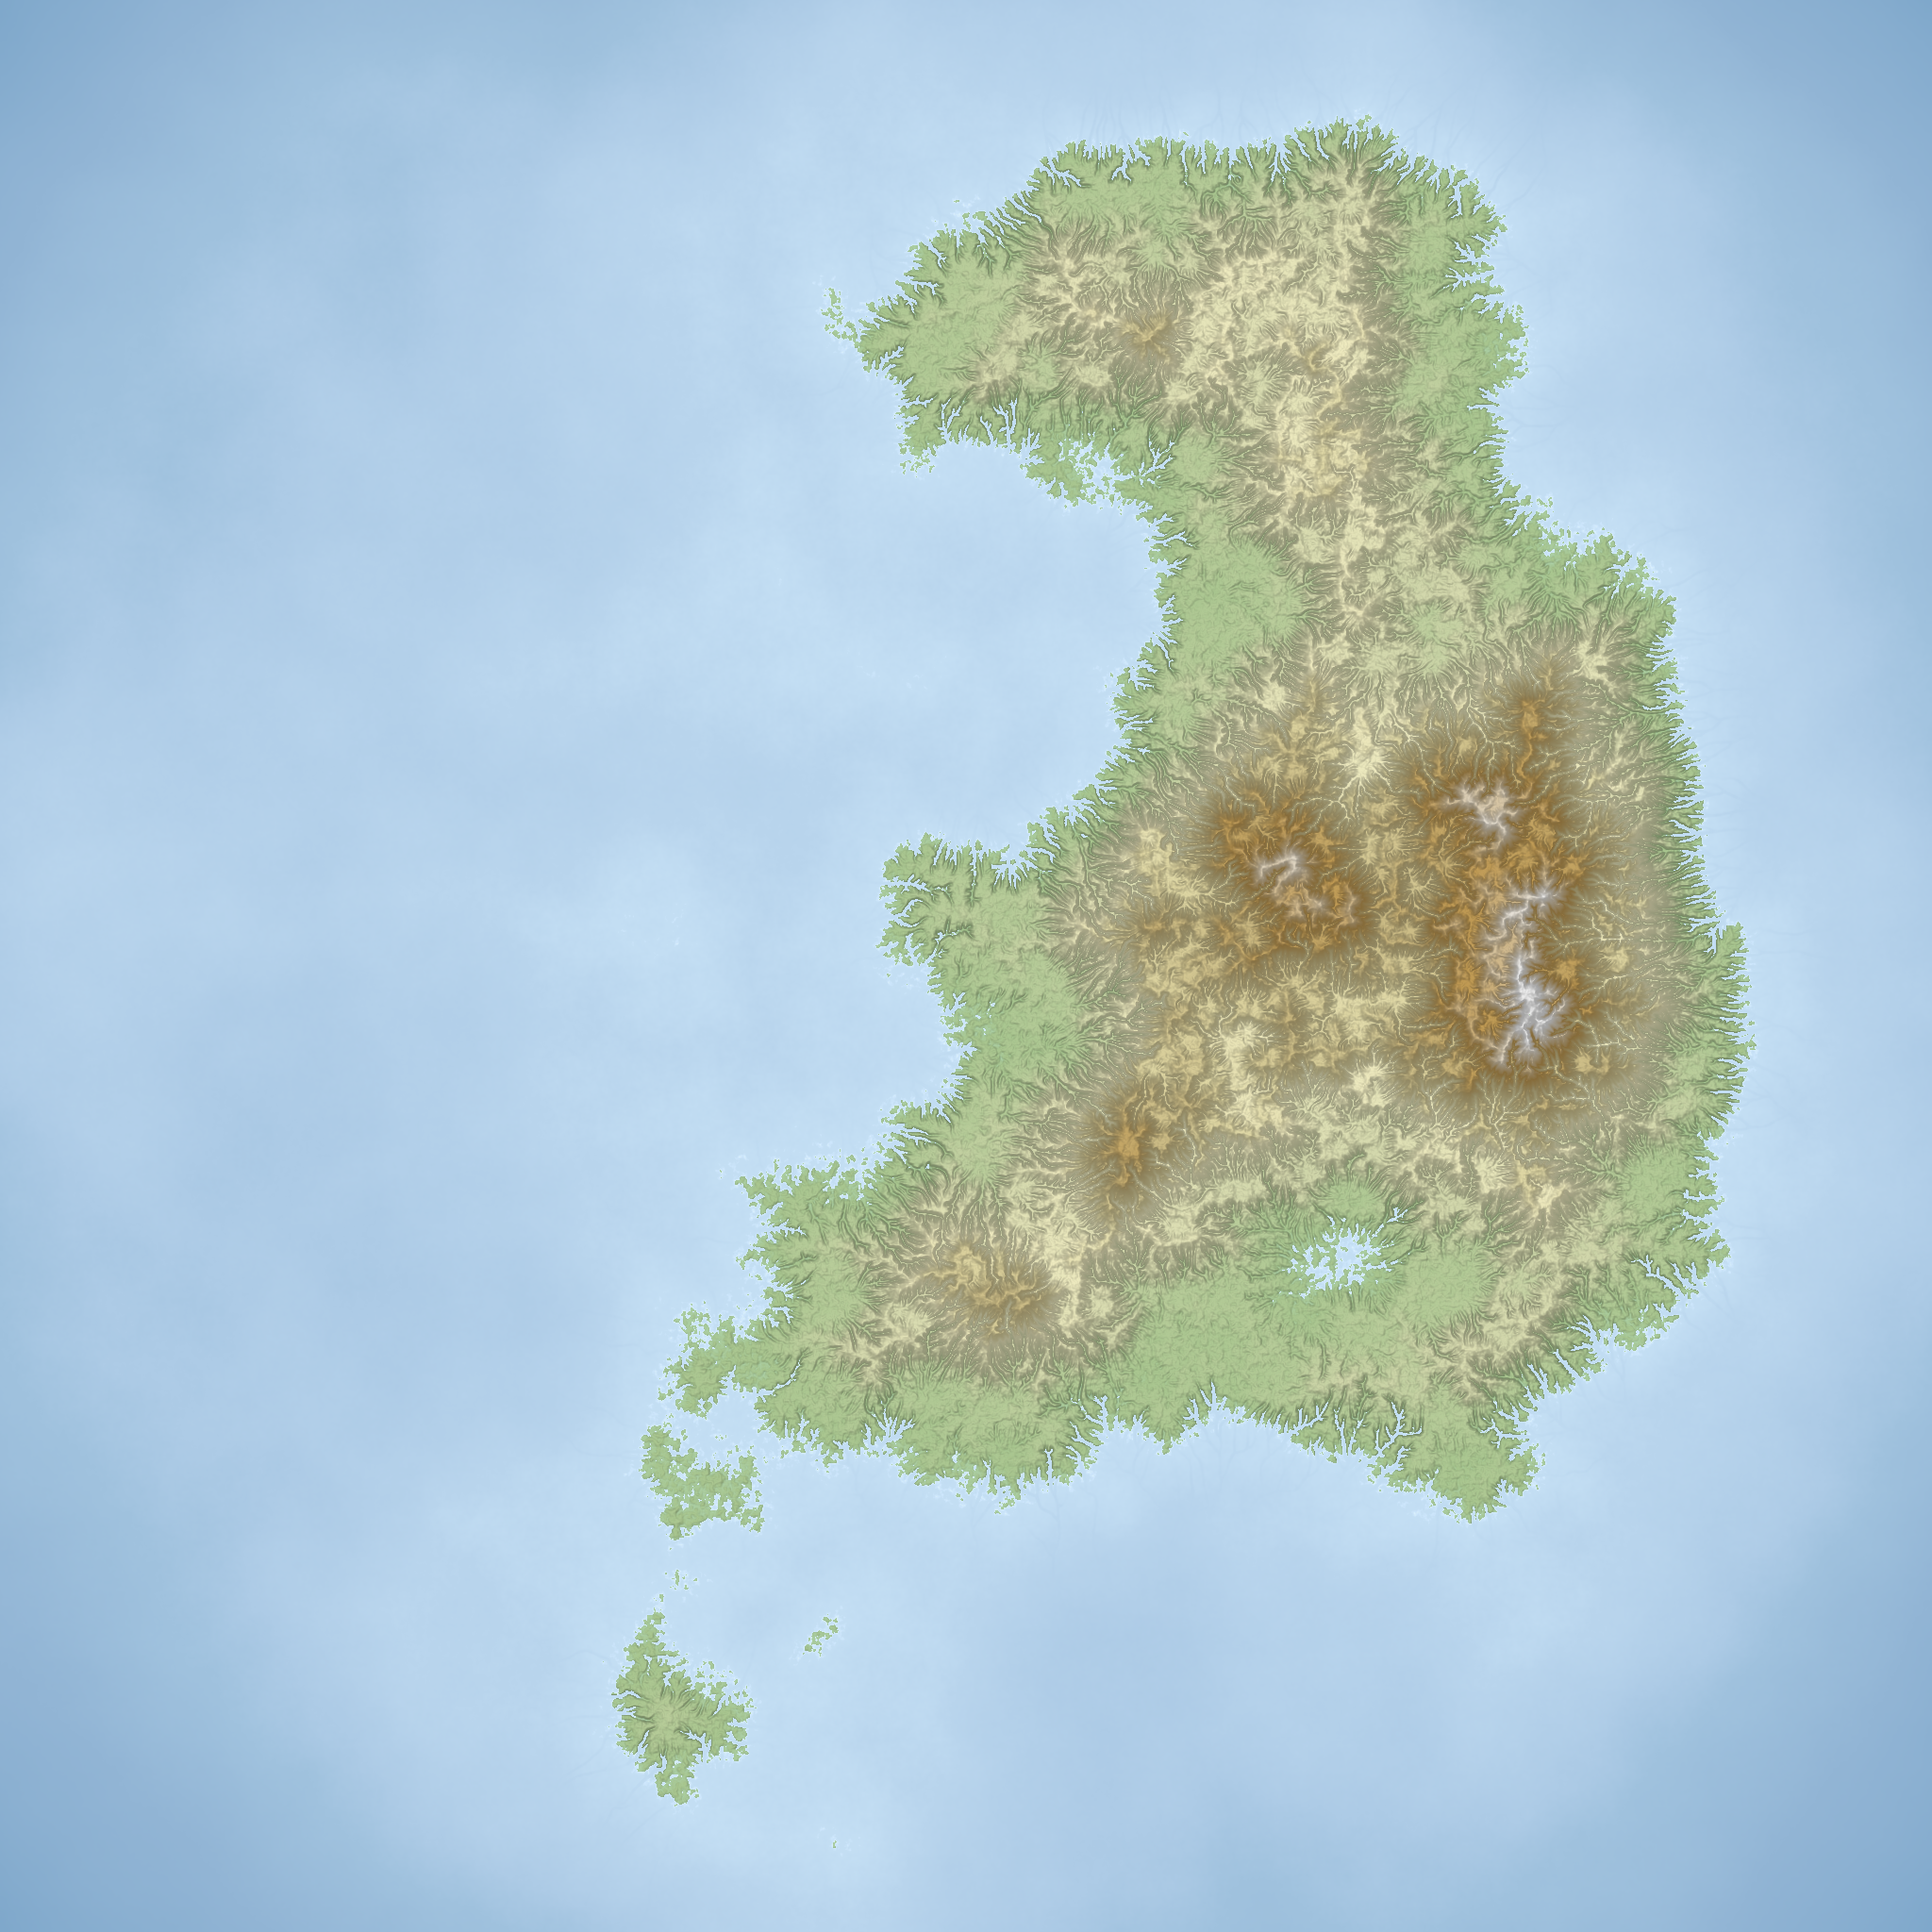
\includegraphics[width=0.8\textwidth]{data/86_rendered.png}}

\ods
Úlohu si rozdelíme na menšíe časti a o každej z nich si niečo povieme.
Najprv si  vyrobíme 
výškovú mapu ({\em heightmap}): tabuľku \prg!double! s číslami z rozsahu
$0\ldots1$, kde $0$ znamená najmenšiu a $1$ najväčšiu výšku (obrázok A).
Z nej potom urobíme dva obrázky: jeden, ktorý bude určovať farbu získame tak,
že každému pixelu priradíme farbu z nejakého gradientu podľa jeho výšky (obrázok B)
a druhý, ktorý bude určovať tiene, vyrobíme  podľa sklonu terénu (obrázok C). Napokon
oba obrázky spojíme do výsledku (obrázok D).


\ods
\centerline{
  \begin{tikzpicture}[scale=5]
    \def\tmp#1{\includegraphics[width=3.8cm]{data/86_#1.png}}
    \node (A) at (0,0) {\tmp{heightmap}};
    \node (B) at (1,0) {\tmp{colored}};
    \node (D) at (2,0) {\tmp{rendered}};
    \node (C) at (1,-1) {\tmp{normal}};

    \foreach \a in {A,B,C,D}
    \node [above = of \a, yshift = -11mm] {(\a)};

    \draw[->] (A) -- (B);
    \draw[->] (B) -- (D);
    \draw[->] (A) to[out=270,in=180] (C);
    \draw[->] (C) to[out=0,in=270] (D);
  \end{tikzpicture}}

Začneme s prípravnou prácou: na zapisovanie finálneho výsledku môžeme použiť náš starý súbor
\hbox{\link{\rootpath/obrazok.h}{obrazok.h}.} Okrem toho budeme veľa robiť s tabuľkami,
kde budeme mať buď reálne čísla alebo farby, tak je dobré sa na to pripraviť.

\begin{uloha}
  Uprav triedu {\tt Tabulka} z kapitoly \ref{sect:cukor} tak, aby sa v nej 
  dali ukladať akékoľvek typy (pomocou šablóny).
\end{uloha}

Prvý pokus o náhodnú výškovú mapu môže vyzerať nejak takto\footnote{%
Tu idem použiť zápis, ktorý sme doteraz nemali a zaslúži si komentár. Ak mám napr. premennú
\prg!int i!, tak vieš, že \prg!i++! je príkaz, ktorý priráta k \prg!i! jednotku. Doteraz som ti
nepovedal, že \prg!i++! sa dá použiť aj ako výraz. Keby som mal napr. \prg!vector<int> a!,
tak \prg!int x = a[i++]! znamená \cmd{Do \prg!x! ulož hodnotu \prg!a[i]! a potom zvýš \prg!i! o jednotku}.
Je to teda to isté, ako keby som napísal \prg!x = a[i]; i = i+1;!.
Niekedy si možno zbadal aj zápis \prg!++i!, ktorý sám osebe robí to isté, t.j. pripočíta k \prg!i! jednotku,
ale urobí to na začiatku. Preto \prg!int y = a[++i]! je to isté ako \prg!i = i+1; y = a[i];!
}

\begin{lstlisting}
#include <algorithm>
#include <chrono>
#include <cstdlib>
#include <fstream>
#include <iostream>
#include <vector>
#include <sstream>

#include "obrazok.h"
#include "tabulka.h"

using namespace std;
using namespace chrono;

double rnd() { return (double)(random() % (1 << 30)) / (double)(1 << 30); }

void zapis(Tabulka<double>& T, const char* fname) {
  vector<unsigned char> data(T.m * T.n * 4);
  for (int i = 0; i < T.m; i++)
    for (int j = 0; j < T.n; j++) {
      int offs = 4 * ((T.n - j - 1) * T.n + i);
      for (int k = 0; k < 3; k++)
        data[offs++] = 255.0 * T(i, j);
      data[offs++] = 255;
    }
  zapis_rgba_png(T.n, T.m, data.data(), fname);
}

int main(int argc, char** argv) {
  unsigned long seed =
      duration_cast<milliseconds>(system_clock::now().time_since_epoch())
          .count();
  if (argc > 1) {
    stringstream ss(argv[1]);
    ss >> seed;
  } else {
    cout << "vygenerovany seed: " << seed << endl;
  }
  srandom(seed);

  int n = 1024;
  Tabulka<double> T(n, n);
  for (int i = 0; i < n; i++)
    for (int j = 0; j < n; j++) T(i, j) = rnd();

  zapis(T, "sum.png");
}
\end{lstlisting}

\ods
V tomto programe som si spravil pomocné funkcie {\tt rnd()}, ktorá vráti (pseudo) náhodné číslo
ako \prg!double! z rozsahu $0\ldots1$ a {\tt zapis()}, ktorá zoberie tabuľku s výškovou mapou
a zapíše z nej obrázok do súboru tak, že nula je čierna a jednotka je biela. Pri zapisovaní 
obrázka potrebujem na jeden pixel štyri byty {\tt r,g,b,a}. Keďže chcem vyrobiť odtiene sivej,
hodnoty {\tt r,g,b} nastavím všetky rovnako, a to na hodnotu {\tt 255 * T(i,j)}.

\ods 
V hlavnom programe najprv nastavím seed podľa hodiniek ako v predchádzajúcej kapitole. Potom 
sa pozriem, či nie je na príkazovom riadku parameter a ak je, zoberiem ho ako seed. Ak budem 
chcieť zopakovať ten istý ostrov, stačí zadať rovnaký seed. Spustím program a výsledok je


\ods
\centerline{\begin{tikzpicture}[scale=0.8]

  \coordinate (A) at (-2mm,-2mm);
  \coordinate (B) at (4cm, 1cm);
  \draw[red] (A) -- (B);
  \filldraw[draw=red, fill=white] (A) circle (1mm) (B) circle (2.5cm);

  \node[anchor=north east] at (0,0) {
\includegraphics[width=6cm]{data/sum.png}};
  \node at (B) {
\includegraphics[width=2.6cm]{data/sum_big.png}};
  \draw[draw=red] (A) circle (1mm) (B) circle (2.5cm);
\end{tikzpicture}}

\ods
Ugh. Zväčšený roh vpravo ukazuje, prečo to nefunguje: keďže každý pixel je 
nezávislé náhodné číslo, nie je medzi nimi žiaden vzťah. Hodnoty medzi jednotlivými
pixelmi skáču tak, že výsledkom, keď sa naňho pozerám trochu z diaľky, je sivá plocha.
Potrebujem niečo, čo by síce bolo náhodné, ale zasa nie až tak úplne. Ukážem ti 
jednu z možností, ako náhodnosť regulovať. Volá sa podľa chlapíka, čo s tým prvý prišiel,
{\em Perlin noise}. S ním sa dajú generovať rôzne veľké náhodné vzory, ktorých kombináciou
vznikajú fraktálovité náhodné útvary.

\ods
% perlin 17
\centerline{\begin{tikzpicture}[scale=3.4]
  \foreach \i in {0,1} {
    \foreach \j in {0,1,2} {
      \pgfmathtruncatemacro{\tmp}{1+3*\i+\j}
      \node at (\j,-\i) {\includegraphics[width=31mm]{data/sample_perlin_\tmp.png}};
      }}

  \node[draw, single arrow, minimum height=12mm, minimum width=8mm,
  single arrow head extend=2mm, anchor=center] at (2.75,-0.5) {};

      \node at (3.5,-0.5) {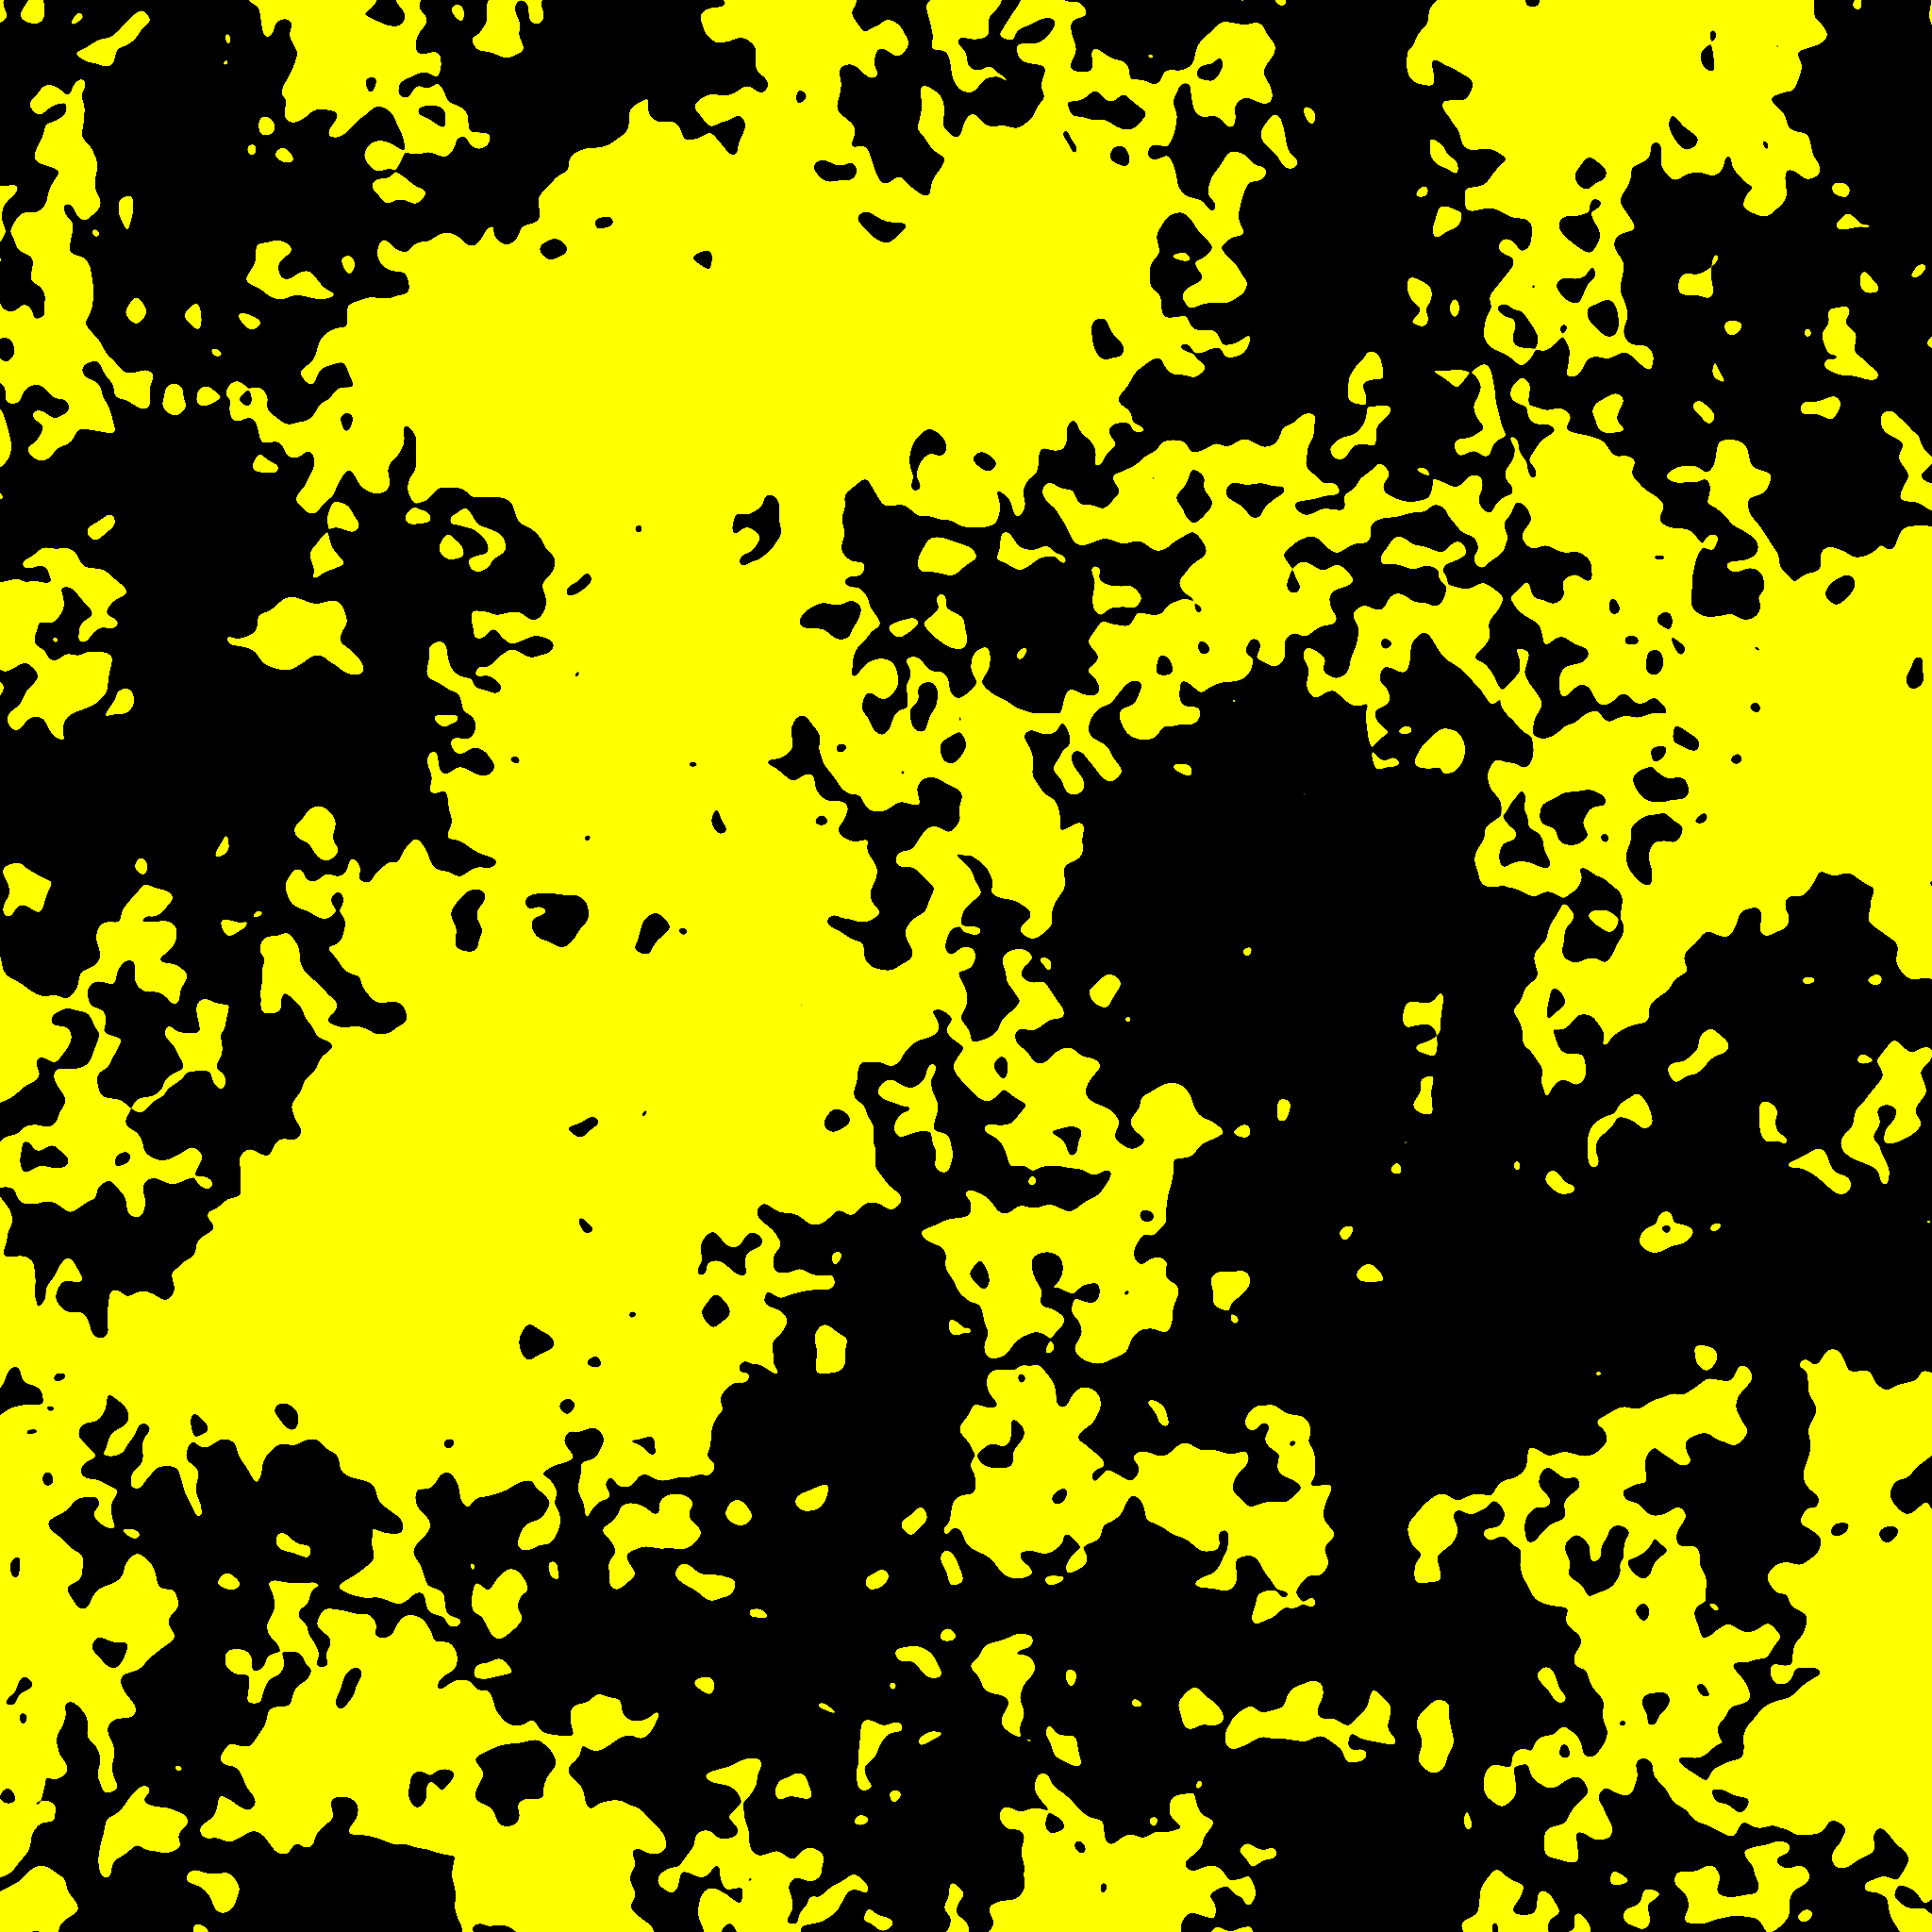
\includegraphics[width=3cm]{data/sample_perlin.png}};
      
\end{tikzpicture}}


\ods
Perlin noise najprv popíšeme matematicky a potom sa pozrieme na to, ako ho naprogramovať.
Zoberme si rovinu. Každému bodu chceme priradiť číslo tak, že čísla menšie ako $-1$ znamenajú
čiernu, čísla väčšie ako $1$ bielu a medzi nimi je spojitý prechod. Budeme tak dostávať 
obrázky ten nasledujúci ako vľavo. Keby sme chceli vzorku ako tá vpravo, môžeme každý bod zaokrúhliť: ak je
kladný, pixel bude žltý, ak je záporný, pixel bude čierny.

\centerline{
  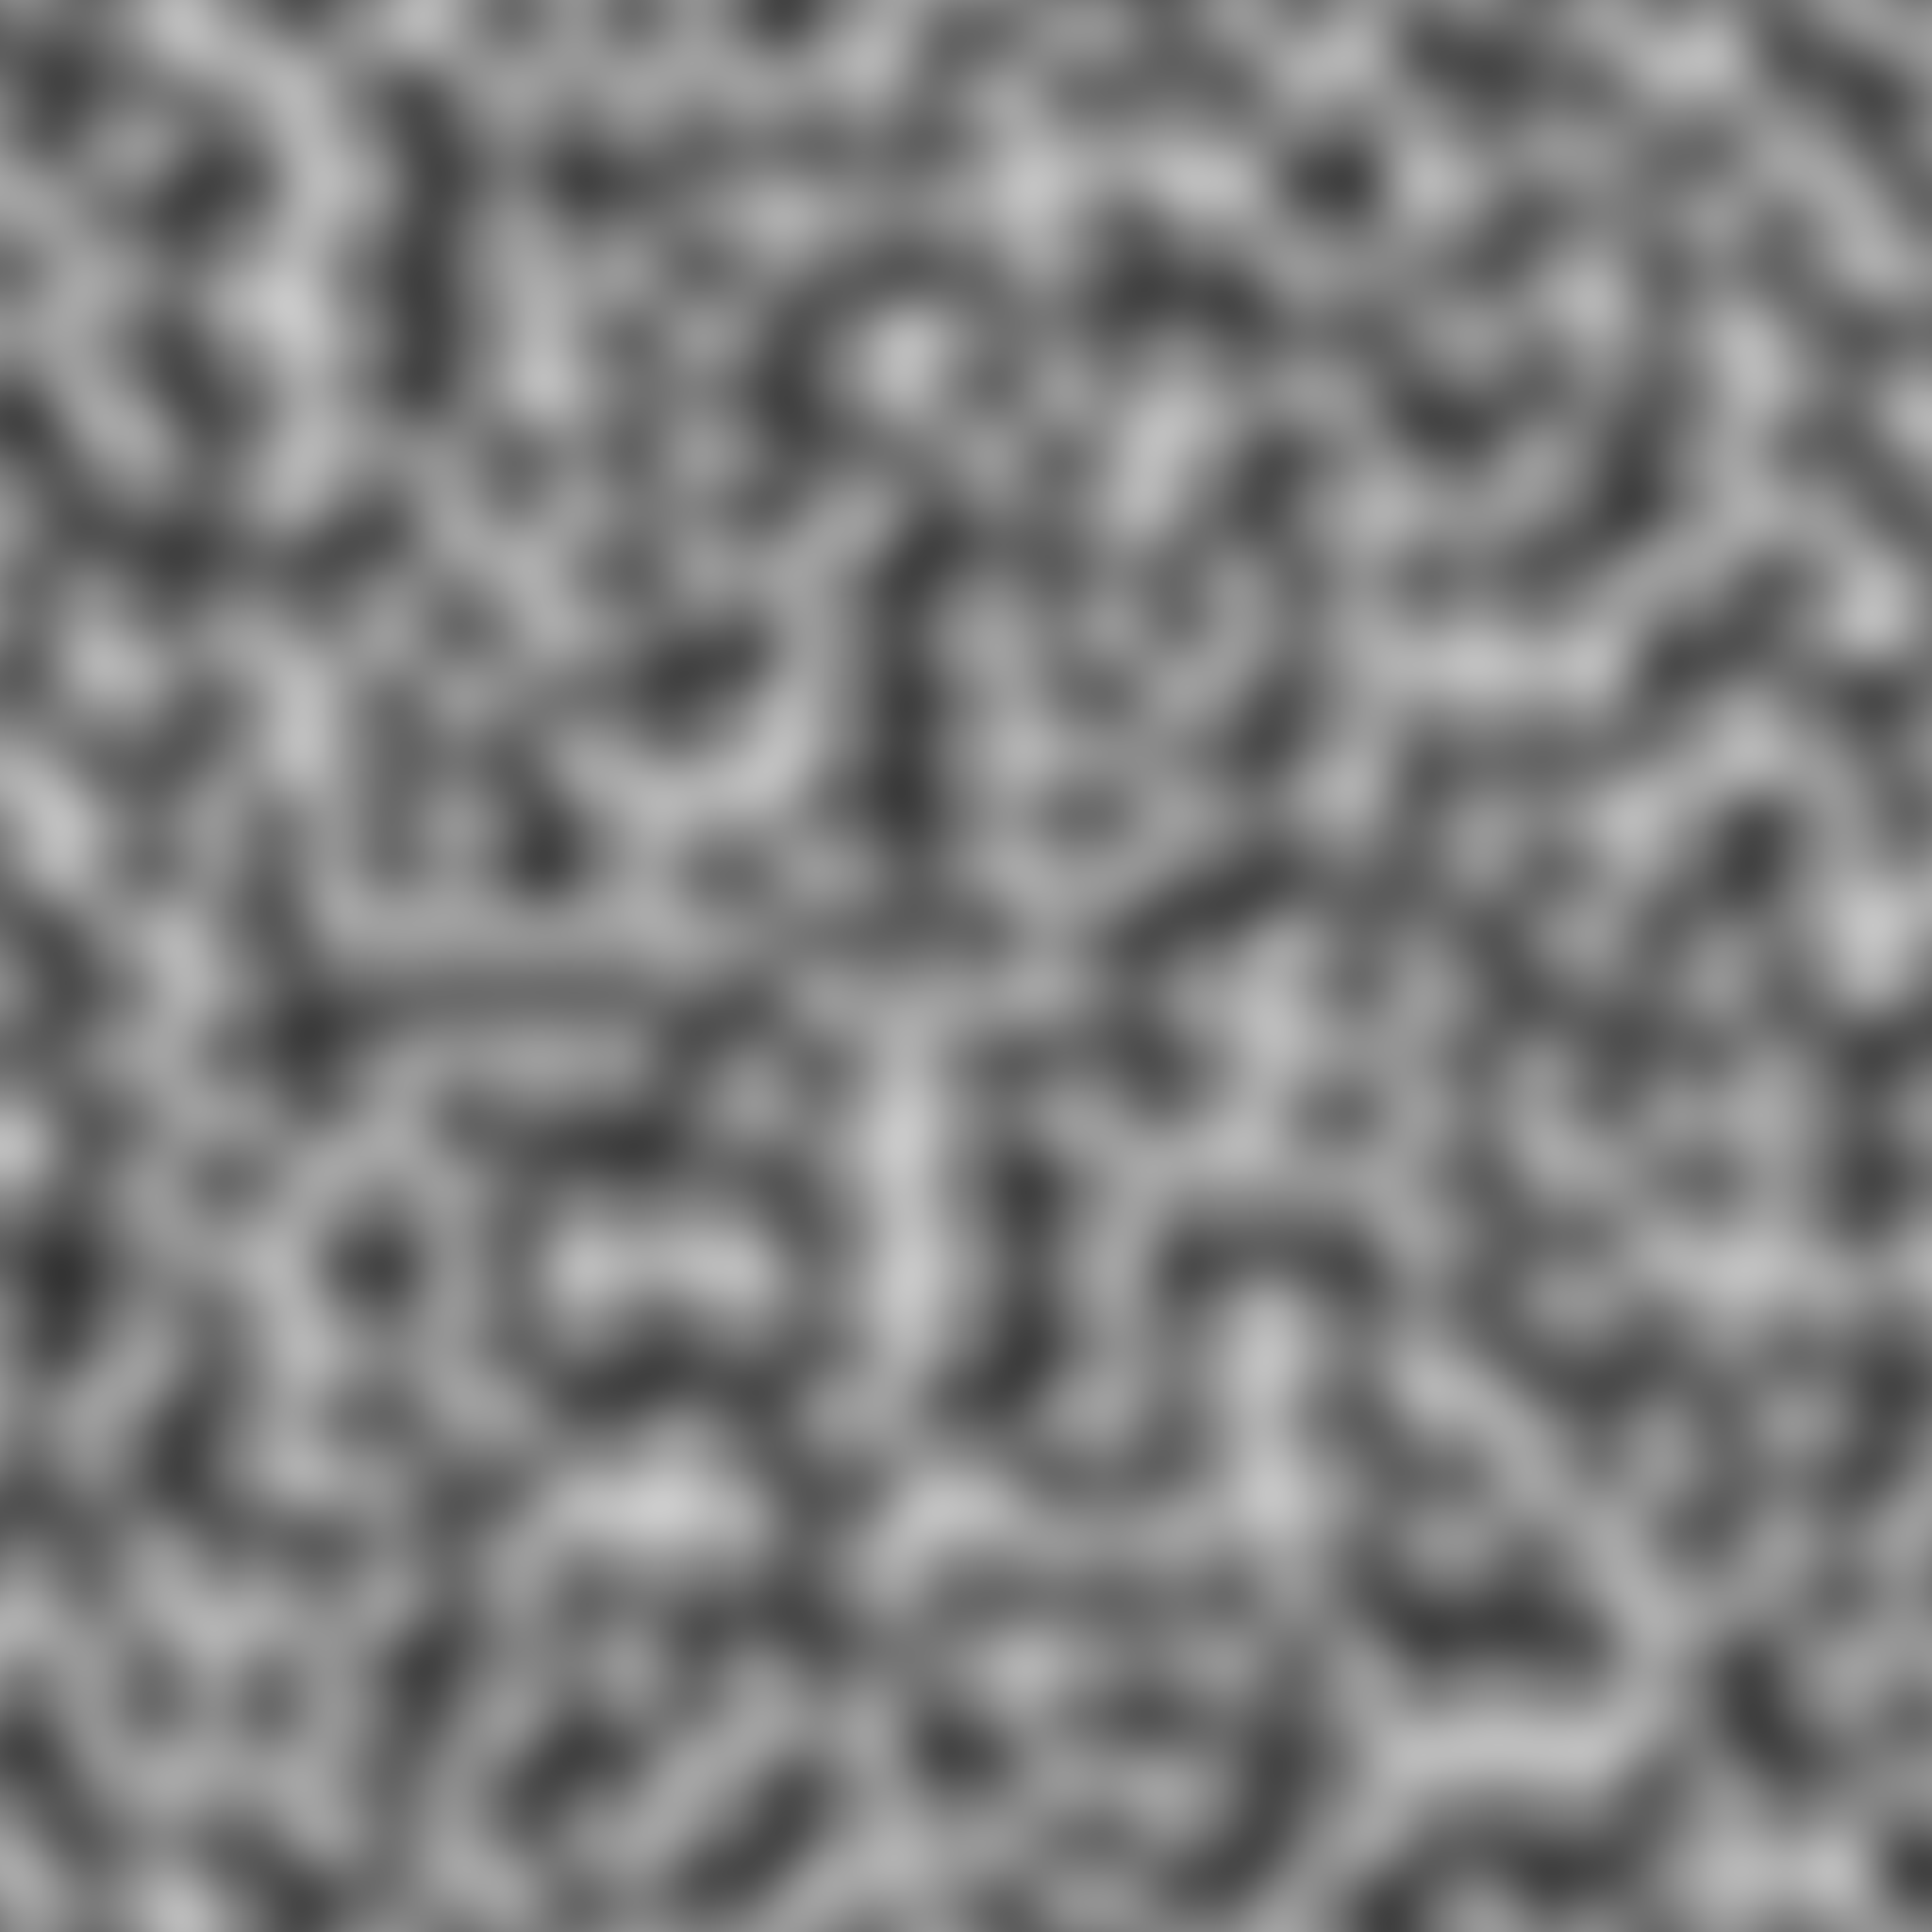
\includegraphics[width=0.4\textwidth]{data/perlin_single.png}
  \hskip 1cm
  
\includegraphics[width=0.4\textwidth]{data/perlin_single_crisp.png}
}

\ods
Základom pre vyrobenie obrázka vľavo je "natočený gradient". Zoberiem si nejaký bod $P$  a 
umiestnim doňho natočenú šípku. Tento gradient každému bodu v rovine 
priradí hodnotu podľa jeho pozície 
v smere šípky. Napr. ak mám šípku umiestnenú v bode $P=[-0.5,0.5]$, tak bodu $A$ sa
priradí číslo $0.7$ a bodu $B$ číslo $-0.4$.


\ods
\centerline{\begin{tikzpicture}[scale=1.5]
  \def\targetfill(#1)[#2]{% 
    \begin{scope}[shift={(#1)},rotate=#2]
    \shade[shading=axis,top color=white, bottom color = black, shading angle=40] 
    (0,0) circle (1);
  \end{scope}
  }
  \def\target(#1)[#2]{% 
    \begin{scope}[shift={(#1)},rotate=#2]
    \draw[red] (0,0) circle (1) (-1.5,0) -- (1.5,0);
  \draw[red,->] (0,-1.5) -- (0,1.5);
    \fill [red] (0,0) circle (0.35mm);
  \end{scope}
  }

  \def\point(#1)[#2]#3#4#5#6#7#8{
    \begin{scope}[shift={(#1)},rotate=#2]
      \coordinate (#5) at (0,#3);   
    \fill[#6] (#5) circle (0.35mm);
      \filldraw[#6, fill=#6, dashed] (#5) node[anchor=#7] {$#3$} -- ++(#4,0) 
      circle (0.35mm) node[anchor=south #8, black]{$#5$};
  \end{scope}
  }

  \coordinate (P) at (-0.5,0.5);
  \targetfill(P)[20]
  \draw[help lines, color=gray!30, dashed] (-2.9,-1.9) grid (2.9,2.9);
  \draw[->] (-3,0) -- (3,0) node[right] {$x$};
  \draw[->] (0,-2) -- (0,3) node[above] {$y$};
  \target(P)[20]
  \node[anchor=north east, red] at (P) {$P$};
  \point(P)[20]{0.7}{2.5}{A}{blue}{east}{west}
  \point(P)[20]{-0.4}{-1.5}{B}{green}{west}{east}

\end{tikzpicture}}

Výsledný obrázok získame tak, že si v rovine spravíme pravidelnú mriežku, 
v ktorej umiestnime náhodne otočené gradienty.
Každý bod roviny leží v nejakom štvorci mriežky a jeho výsledná farba sa určí kombináciou farieb zo
štyroch susedných gradientov.

\ods
\centerline{\begin{tikzpicture}[scale=3]
  \def\sza{0.2}
  \def\szb{0.36}
  \def\target(#1)[#2]{% 
    \begin{scope}[shift={(#1)},rotate=#2]
    \draw[red] (0,0) circle (\sza) (-\szb,0) -- (\szb,0);
  \draw[red,->] (0,-\szb) -- (0,\szb);
    \fill [red] (0,0) circle (0.15mm);
  \end{scope}
  }
  \node at (1,1) {
\includegraphics[width=6cm]{data/perlin_fixed.png}};
  \draw[help lines,color=gray!30, dashed] (0,0) grid (2,2);

  %perlin 12
  \foreach \x/\y/\a in 
  {0/0/80,0/1/140,0/2/140,1/0/280,1/1/190,1/2/30,2/0/170,2/1/90,2/2/130} {
    \target(\x,\y)[\a-90]
  }

  \coordinate (A) at (1.6,1.35);
  \filldraw[blue, dashed] (A) node[anchor=north] {$P$} circle (0.15mm) -- (1,1) (A) -- (1,2) (A) -- (2,1) (A) -- (2,2);
\end{tikzpicture}}

\ods
Kombináciu hodnôt urobíme podobne, ako sme robili interpoláciu farieb vo farebnom
gradiente v projekte o Mandelbrotovej množine,
až na to, že teraz potrebujeme interpolovať v dvoch rozmeroch (preto sa tomu hovorí {\em bilineárna interpolácia}).
Predstav si, že máme mriežku gradientov s krokom $d$ a chceme určiť farbu pre bod $P$ so súradnicami $[x,y]$.
Keď si všetky súradnice vydelím $d$čkom, mriežka bude mať krok $1$.
$P$ sa nachádza v mriežke medzi štyrmi bodmi $G_{00}$, $G_{10}$, $G_{01}$ a $G_{11}$.
Pripomeniem, že $\lfloor x\rfloor$ označuje celú časť z $x$, preto $G_{00}$ má súradnice
$\left\lfloor\frac{x}{d}\right\rfloor,\left\lfloor\frac{y}{d}\right\rfloor$ a ostatné 
4 body sú vždy o $1$ ďalej.

\ods
\centerline{\begin{tikzpicture}[scale=5.5]
  \def\ofs{0.2}
  \def\ofsi{0.35}
  \def\lclr{teal}
  \tikzstyle{link}=[dashed, thin, \lclr, shorten <= -0.6ex]
  \def\dot(#1)[#2]{\fill[#2] (#1) circle (0.007);}
  % pozicia, uhol, dlzka od-do, vyska, nazov suradnice
  \def\grr(#1)[#2](#3,#4)#5{
    \begin{scope}[shift={(#1)},rotate=#2]
      \draw[red] (-0.1,0) -- (0.1,0) (0,0) circle (0.05);
      \draw[->,red] (0,#3) -- (0,#4);
      \coordinate (#5) at ($(0,-100)!(P)!(0,100)$);
    \end{scope}
  }
  \draw[dashed] (0,0-\ofsi) node [below] {$\left\lfloor\frac{x}{d}\right\rfloor$} -- (0,0);
  \draw[dashed] (1,0-\ofsi) node [below] {$\left\lfloor\frac{x}{d}\right\rfloor+1$} -- (1,0);
  \draw[dashed] (1+\ofsi,0) node [right] {$\left\lfloor\frac{y}{d}\right\rfloor$} -- (1,0);
  \draw[dashed] (1+\ofsi,1) node [right] {$\left\lfloor\frac{y}{d}\right\rfloor+1$} -- (1,1);

  \draw (0-\ofs,0) -- (1+\ofs,0) (0-\ofs,1) -- (1+\ofs,1) (0,0-\ofs) -- (0,1+\ofs) (1,0-\ofs) -- (1,1+\ofs);
  \node[anchor = north east, inner sep=0.5cm] at (0,0) {$G_{00}$} ;
  \node[anchor = north west, inner sep=0.5cm] at (1,0) {$G_{10}$} ;
  \node[anchor = south east, inner sep=0.5cm] at (0,1) {$G_{01}$} ;
  \node[anchor = south west, inner sep=0.5cm] at (1,1) {$G_{11}$} ;
  

  \coordinate (P) at (0.43,0.6);
  
  \grr(0,0)[19](-0.15,0.5){v00} 
  \draw[link] (v00) node[anchor=north west] {$v_{00}$} -- (P);
  \dot(v00)[\lclr]
  
  \grr(1,0)[-30](-0.15,0.3){v10}
  \draw[link] (v10) node[anchor=north west] {$v_{10}$} -- (P);
  \dot(v10)[\lclr]

  \grr(0,1)[-62](-0.15,0.3){v01}
  \draw[link] (v01) node[anchor=south east] {$v_{01}$} -- (P);
  \dot(v01)[\lclr]

  \grr(1,1)[-130](-0.3,0.2){v11}
  \draw[link] (v11) node[anchor=south west] {$v_{11}$} -- (P);
  \dot(v11)[\lclr]


  \draw[blue,brace=1mm/](0,1.2)-- node[above=2.5ex]{$1$}(1,1.2);

  \coordinate (Px) at ($($(0,0)!(P)!(1,0)$) + (0,0-\ofs)$);
  \coordinate (Py) at ($($(0,0)!(P)!(0,1)$) + (0-\ofs,0)$);
 
  \draw[thin,lightgray]  (Px) -- ($(0,1)!(P)!(1,1)$)  (P)--(Py);
  \draw[blue,brace=1mm/mirror] (0,0-\ofs) -- node[below=2.5ex]{$r=\frac{x}{d}-\left\lfloor\frac{x}{d}\right\rfloor$} (Px);
   \draw[blue,brace=1mm/mirror] (Px) -- node[below=2.5ex]{$1-r$} (1,0-\ofs);

   \draw[blue,brace=1mm/] (0-\ofs,0) -- node[left=2.5ex]{$s=\frac{y}{d}-\left\lfloor\frac{y}{d}\right\rfloor$} (Py);
   \draw[blue,brace=1mm/] (Py) -- node[left=2.5ex]{$1-s$} (0-\ofs,1);

  \dot(P)[black]
  \node[anchor=west] at (P){$P\;\left[\frac{x}{d},\frac{y}{d}\right]$};
  \fill ($(0,0)!(P)!(1,0)$) node[anchor = north west]{$C$} circle (0.007)
   ($(0,1)!(P)!(1,1)$) node[anchor = south west]{$D$} circle (0.007);
\end{tikzpicture}}
\pagebreak[1]

\ods
Predpokladajme, že sme už vyrátali hodnoty, ktoré prislúchajú bodu $P$ v
jednotlivých gradientoch a označili sme si ich
$v_{00}$, $v_{10}$, $v_{01}$ a $v_{11}$. Ako z nich skombinovať výslednú hodnotu v $P$? 
Desatinná časť po vydelení $x/d$ 
je $r=\frac{x}{d}-\left\lfloor\frac{x}{d}\right\rfloor$. Keby si bod $P$
posúval v štvorci zľava doprava, hodnota $r$ sa bude plynule meniť medzi $0$ a $1$.
Preto hodnotu v bode $C$ vieme interpolovať ako $v_C=v_{00}(1-r)+v_{10}r$. 
Podobne hodnotu v bode $D$ interpolujeme
$v_D=v_{01}(1-r)+v_{11}r$. 
Napokon urobíme rovnakým spôsobom interpoláciu medzi $v_C$ a $v_D$ v smere osi $y$, 
takže výsledok bude $v_C(1-s)+v_Ds$. 

\ods
Skoro dobré, ale  je tam stále drobný
problém: pretože interpolujeme lineárne iba v rámci jedného štvorca,
vznikajú nám nepekné zlomy ako vľavo, kým my potrebujeme hladký prechod ako vpravo

\ods
\centerline{
  
\includegraphics[width=0.4\textwidth]{data/perlinL_fixed.png}
  \hskip 1cm
  
\includegraphics[width=0.4\textwidth]{data/perlin_fixed.png}
}

\phantom{a}
\hfill
\begin{tikzpicture}
\begin{axis}[
  width=60mm, 
  height=6cm,
  domain=0:1,
  xmin=0,
  xmax=1,
  ymin=0,
  ymax=1,
  xlabel=$r$,
  /pgf/number format/.cd,
        1000 sep={}
]
  \addplot[no markers,red!50!white]{x};
  \addplot[no markers,green!50!white]{1-x};
\end{axis}
\end{tikzpicture}
  \hfill
\begin{tikzpicture}
\begin{axis}[
  width=60mm, 
  height=6cm,
  domain=0:1,
  xmin=0,
  xmax=1,
  ymin=0,
  ymax=1,
  xlabel=$6r^5-15r^4+10r^3$,
  /pgf/number format/.cd,
        1000 sep={}
]
  \addplot[no markers,red!50!white]{x * x * x * (10 + x * (6 * x - 15))};
  \addplot[no markers,green!50!white]{1-x * x * x * (10 + x * (6 * x - 15))};
\end{axis}
\end{tikzpicture}
\hfill
\phantom{a}

\ods
Hladký prechod sa dá dosiahnuť tak, že namiesto interpolácie s parametrami $r$ a $1-r$, ktoré
sú pri koncoch špicaté, budeme interpolovať s parametrami $f(r)$ a $1-f(r)$ pre nejakú
vhodnú funkciu $f$, ktorá je na koncoch hladká. Perlin odporúča zobrať 
$f(r)=6r^5-15r^4+10r^3$. Môžeme aj tak, prečo nie.

\ods 
Teraz môžeme napísať takmer celý program na Perlin noise. 
Najprv si urobím pomocnú funkciu na lineárnu interpoláciu {\tt lerp}, ktorá sa
bude hodiť vo všeobecnejšej podobe

\ods
\begin{lstlisting}
template <typename T>
T lerp(const T& v0, const T& v1, double t) {
  return (1 - t) * v0 + t * v1;
}
\end{lstlisting}

\ods
Teraz vyrobím triedu {\tt Perlin},
ktorá bude mať dva parametre: {\tt n} veľkosť obrázka (pre jednoduchosť budem
robiť štvorcové obrázky rozmerov $n\times n$) a krok mriežky {\tt d}.
Zavolanie konštruktora vyrobí tabuľku {\tt H}, v ktorej bude výsledná výšková
mapa. Na natočené šípky budem mať triedu {\tt Vec} o ktorej si povieme viac o 
chvíľu, nateraz si ju predstav ako 

\ods
\begin{lstlisting}
struct Vec {
  double x, y;
};
\end{lstlisting}

\ods
Natočené šípky budú uložené v tabuľke $H$ rozmerov $m\times m$, kde 
$m=1+\left\lfloor\frac{n}{d}\right\rfloor$. V konštruktore
najprv vygenerujeme náhodné šípky tak, že zvolíme náhodný uhol {\tt theta} ($\theta$)
a šípka bude ukazovať do bodu so súradnicami $[\cos(\theta),\sin(\theta)]$
(o funkciách $\sin$ a $\cos$ pozri odbočku v kapitole~\ref{sect:editor}).
Potom už len vyrátam pre každý bod $P=[i,j]$ jeho farbu.
To znamená, že keď vyrobím premennú typu {\tt Perlin}, konštruktor vyrobí tabuľku {\tt H},
ku ktorej potom môžem pristupovať.

\ods
\begin{lstlisting}
struct Perlin {
  int n, d, m;  
  Tabulka<double> H;
  Tabulka<Vec> G;

  Perlin(int _n, int _d) : n{_n}, d{_d}, m{1 + n / d}, 
                           H(n, n), G(m, m) {
    for (int i = 0; i < m; i++)
      for (int j = 0; j < m; j++) {
        double theta = rnd() * M_PI * 2.0;
        G(i, j) = {cos(theta), sin(theta)};
      }

    for (int i = 0; i < n; i++)
      for (int j = 0; j < n; j++) {
        // bod P so suradnicami [i,j]
        Vec p{ (double)i / (double)d,  (double)j / (double)d};

        // suradnice bodu G00
        int o[2] = {(int)p.x, (int)p.y}; 

        // hodnoty v00, v10, v01 a v11
        double v[4];

        ... // tu ich treba nejak vyratat
        
        double r = fade(p.x - o[0]), s = fade(p.y - o[1]);
        double vc = lerp(v[0], v[1], r), vd = lerp(v[2], v[3], r);
        H(i, j) = lerp(vc, vd, s);
      }
  }

  // fade funkcia, ako ju odporucal Perlin
  double fade(double t) {
    return t * t * t * (10 + t * (6 * t - 15));
  }
};
\end{lstlisting}

\ods
Ostáva doplniť posledná vec, a to ako vyrátať hodnoty $v_{00},\ldots,v_{11}$,
teda ako pre daný bod zrátať jeho výšku v nejakom natočenom gradiente. 
Predtým sa ale hodí

\subsection*{Matematické intermezzo: o bodoch a vektoroch}

Bod v rovine je vec, ktorá má dve súradnice, $x$ a $y$. Ak mám dva body, napr.
$A[x,y]$, $B[x',y']$, tak najkratšia cesta z bodu $A$ do bodu $B$ je úsečka, ktorá
sa v smere osi $x$ pohne o $x'-x$ a v smere osi $y$ o $y'-y$. Takýto úsečka
sa volá prenášač 
({\em vektor}) a dá sa zapísať dvoma číslami pre posun v $x$-ovom
a $y$-ovom smere, takže vyzerá
rovnako ako bod so súradnicami $[x'-x,y'-y]$. Je preto prirodzené
si to predstaviť tak, že ak odčítam od seba dva body, dostanem vektor.
Ak treba body a vektory rozlíšiť, nad vektory sa niekedy
zvykne písať šípka, napr. vektor $v$ je $\vec v = B-A$. 
Podobne keď k nejakému bodu $C$ prirátame vektor $\vec v$, 
dostaneme nový bod (ten, do ktorého nás
vektor prenesie).

\ods
\centerline{
\begin{tikzpicture}[scale=0.5]
  \tikzstyle{vecs}= [-{>[length=2ex,width=1.7ex]}]
  \def\dot(#1){\fill (#1)circle (1.8pt) }
  \draw[dotted,thin,gray] (-1,-1) grid (12,8);
  \coordinate (A) at (1,3);
  \coordinate (B) at (8,6);
  \draw[red,style=vecs](A) -- node[anchor = south east, inner sep=2mm]{$\vec v=B-A$}(B);
  \dot(A) node[anchor=north east]{$A$};
  \dot(B) node[anchor=south west]{$B$};
  \draw[thin, teal, dashed] 
  (A) -- ++(3,-2) coordinate (AA)
  (B) -- ++(3,-2) coordinate (BB);
  \draw[magenta, style = vecs] (AA) -- (BB);
  \dot(AA) node[anchor=north]{$C$};
  \dot(BB) node[anchor=north west]{$C+\vec v$};
  \draw[thin] (-1.5,0) -- (12.5,0) (0,-1.5) -- (0,8.5);
\end{tikzpicture}}

Vektory môžeme sčitovať prirodzeným spôsobom po zložkách (t.j. 
$[x,y]+[x',y']=[x+x',y+y']$), čo sa dá nakresliť ako skladanie šípok: na konci jednej
nakreslíme druhú:

\ods
\centerline{
\begin{tikzpicture}[scale=0.5]
  \tikzstyle{vecs}= [-{>[length=2ex,width=1.7ex]}]
  \def\dot(#1){\fill (#1)circle (1.8pt) }
  \draw[dotted,thin,gray] (-1,-1) grid (12,8);
  \coordinate (A) at (1,1);
  \coordinate (B) at ($(A)+(6,2)$);
  \coordinate (C) at ($(B)+(3,5)$);
  \dot(A); \dot(B); \dot(C);
  \draw[orange,style=vecs](A) -- node[anchor = north west, inner sep=1mm]{$\vec u=[6,2]$}(B);
  \draw[teal,style=vecs](B) -- node[anchor = north west, inner sep=1mm]
  {$\vec v=[3,5]$}(C);
  \draw[magenta,style=vecs](A) -- node[anchor = south east, inner sep=1mm]
  {$\vec u+\vec v=[9,7]$}(C);
  \draw[thin] (-1.5,0) -- (12.5,0) (0,-1.5) -- (0,8.5);
\end{tikzpicture}}

\ods
Rovnako dobre dáva zmysel, aby sme vektor vynásobili číslom: napr. ak 
$\vec v=[x,y]$, tak $4.2\cdot\vec v=[4.2x,4.2y]$ je
šípka v rovnakom smere ako $\vec v$, iba $4.2$-krát dlhšia. Podobne $-0.5\cdot\vec v$ je
šípka polovičnej dĺžky a v opačnom smere. 

\ods
Ak mám bod $A[x,y]$, tak si viem povedať, že to je vlastne vektor $A-[0,0]$, t.j.
šípka, ktorá ukazuje zo začiatku súradnicovej sústavy do $A$. Teraz je bod a vektor naozaj
to isté. Premysli si to: napr. $[9,7]-[3,5]=[6,2]$ môžem interpretovať tak, že mám bod
so súradnicami $[9,7]$ a bod so súradnicami $[3,5]$, a vektor medzi nimi má súradnice $[6,2]$.
Ale rovnako môžem povedať, že ak mám vektor $[3,5]$, tak $-[3,5]$ je rovnako dlhý vektor v 
opačnom smere a $[9,7]+(-[3,5])$ je skladanie vektorov, ktorého výsledkom je vektor $[6,2]$.

\ods
Z Pytagorovej vety viem, že ak $\vec v$ je vektor so súradnicami $[x,y]$, tak jeho 
dĺžka je $\nrm{\vec v}=\sqrt{x^2+y^2}$. Ak obe súradnice vydelím dĺžkou, dostanem vektor
$\vec v'=\left[\frac{x}{\nrm{\vec v}},\frac{y}{\nrm{\vec v}}\right]$, ktorého dĺžka je 
$$\nrm{\vec v'}=\sqrt{\left(\frac{x}{\nrm{\vec v}}\right)^2+\left(\frac{y}{\nrm{\vec v}}\right)^2}
=\sqrt{\frac{x^2}{\nrm{\vec v}^2}+\frac{y^2}{\nrm{\vec v}^2}}
=\sqrt{\frac{1}{\nrm{\vec v}^2}(x^2+y^2)}=\sqrt{\frac{1}{\nrm{\vec v}^2}}\sqrt{x^2+y^2}=
\frac{1}{\nrm{\vec v}}\nrm{\vec v}=1
$$
Hovoríme, že $\vec v'$ je {\em normovaný} (resp. {\em normalizovaný}) vektor.

\ods
\centerline{
\begin{tikzpicture}[scale=0.5]
  \tikzstyle{vecs}= [-{>[length=2ex,width=1.7ex]}]
  \def\dot(#1){\fill (#1)circle (1.8pt) }
  \draw[dotted,thin,gray] (-1,-1) grid (12,8);
  \coordinate (A) at (9,7);
  \draw[magenta, style=vecs] (0,0) -- (A) node[anchor=south west]{$\vec v = [x,y]$};
  \dot(0,0); \dot(A);
  \draw[thin] (-1.5,0) -- (12.5,0) (0,-1.5) -- (0,8.5);
  \draw[thin,gray](A) -- ($(0,0)!(A)!(10,0)$) coordinate(Ax);
  \draw[brace=1mm/] (A) -- node[anchor=west, xshift=2ex]{$y$} (Ax);
  \draw[thick, teal, style=vecs] (0,0) -- node[anchor=south east]{$1$}
  ($0.4*(A)$) coordinate(B) node[anchor=south east]{$\vec v'$};
  \dot(B);
  \draw[thin,gray](B) -- ($(0,0)!(B)!(10,0)$) coordinate(Bx);
  \draw[brace=1mm/] (B) -- node[anchor=west, xshift=2ex]{$\frac{y}{\nrm{\vec v}}$} (Bx);
\end{tikzpicture}}

\ods
Máme teda vektory, ktoré vieme sčitovať, odčitovať a násobiť reálnym číslom. Samozrejme, toto
všetko by rovnako dobre fungovalo v troch (a viacerých) rozmeroch. Môžeme ale nejak rozumne
vynásobiť dva vektory medzi sebou? 
Tu to už nie je také jednoznačné. Môžme vymyslieť rôzne 
operácie, ktoré nazveme súčin, a ktoré budú mať rôzne vlastnosti podľa toho, čo práve potrebujeme počítať. 
Jeden spôsob je uvedomiť si, že vektor v rovine so súradnicami $[x,y]$
je vlastne komplexné číslo $x+iy$, takže môžeme používať násobenie ako pri komplexných číslach.
Ukážem ti ešte dva iné spôsoby, ktoré sa nám budú hodiť, a to tzv.  {\em skalárny} a {\em vektorový} súčin.

\ods
Skalárny súčin je spôsob násobenia, ktorý je veľmi prirodzený napr. vo fyzike. Možno vieš, že fyzikálna
veličina {\em práca} je súčin sily a dráhy, t.j. ak pôsobí na teleso sila $1$N a posunie ho tým o $1$m,
vykoná pri tom prácu $1$J. Zvyčajne sa to zapisuje $W=Fd$.

\ods
\centerline{
  \begin{tikzpicture}[scale=1] 
  \draw[white] (0,0) -- (0,-0.8);
    \definecolor{acol}{rgb}{0.85,0.85,0.95}
    \node[xscale=-1,yscale=1,inner sep=0pt, anchor = south] (auto) at (2.7,0) {\textcolor{acol}{\usymH{1F69A}{1cm}}};    
    \node[xscale=-1,yscale=1,cyan!50!white,anchor=south, inner sep=0pt] (vlak) at (0,0) {\usymH{1F683}{1cm}};
    \draw[draw=acol, shorten <= 0.68cm, shorten >= 0.5cm, line width=0.6mm] 
    ($(vlak.center)+(0,-0.2)$) -- ($(auto.center)+(0,-0.2)$);
  %\node[xscale=-1,yscale=1,blue,anchor=south, inner sep=0pt] at (5,3) {\usymH{1F681}{1cm}};

    \draw (-1.5,0) -- (6,0);
  \foreach \x in {0,...,5}
  \draw (\x,-0.1) -- (\x,0.1);
    \fill[red] (vlak.center) circle (0.8mm);
    \draw[red,line width=0.6mm,->,>=latex] (vlak.center) -- node[above]{$F$} ++(3,0);
    \draw[cyan,line width = 0.6mm,->,>=latex] (0,-0.4) -- node[below]{$d$} (5,-0.4);
    \fill[cyan] (0,-0.4) circle (0.8mm);

\end{tikzpicture}
}

\ods
Tu sa ale potichu predpokladá, že sila aj dráha sú čísla, a preto ich môžem násobiť. Lenže v skutočnosti sila aj dráha sú
vektory a môžu pôsobiť rôznym smerom

\ods
\centerline{
  \begin{tikzpicture}[scale=1] 
  \draw[white] (0,0) -- (0,-0.8);
    \definecolor{acol}{rgb}{0.85,0.85,0.95}
   % \node[xscale=-1,yscale=1,inner sep=0pt, anchor = south] (auto) at (2.7,0) {\textcolor{acol}{\usymH{1F69A}{1cm}}};    
    \node[xscale=-1,yscale=1,blue,anchor=south, inner sep=0pt] (heli) at (4,2.5) {\textcolor{acol}{\usymH{1F681}{1cm}}};
    \node[xscale=-1,yscale=1,cyan!50!white,anchor=south, inner sep=0pt] (vlak) at (0,0) {\usymH{1F683}{1cm}};
    \draw[draw=acol, shorten <= 0.8cm, shorten >= 0.3cm, line width=0.6mm] 
    (vlak.center) -- ($(heli.center)+(0,-0.3)$) coordinate (lano);

    \draw (-1.5,0) -- (6,0);
  \foreach \x in {0,...,5}
  \draw (\x,-0.1) -- (\x,0.1);
    \draw[cyan,line width = 0.6mm,->,>=latex] (vlak.center) -- node[below]{$\vec d$} ++(5,0) coordinate (endD);
    \draw[red,line width=0.6mm,->,>=latex] (vlak.center) -- node[above]{$\vec F$} ($(vlak.center)!0.8!(lano)$) 
    coordinate(endF);
    \draw[thin, gray, dashed] (endF) -- ($(vlak.center)!(endF)!(endD)$) coordinate(fin);
    \draw[thin, ->, >=latex ] (vlak.center) -- (fin);
    \def\len{0.95cm}
    \draw[thin] ($(vlak.center)!\len!(endD)$) arc(0:28:\len);
    \fill[red] (vlak.center) circle (0.8mm);
\end{tikzpicture}
}

\ods
V tomto prípade sa časť sily, ktorou pôsobí vrtuľník, vyplytvá na nadľahčovanie vagóna a prácu robí 
iba tá časť, ktorá je rovnobežná s dráhou, takže na vyrátanie práce násobím
dĺžku vektora $\vec d$ a priemetu $\vec F$ (čierna šípka na obrázku). 
Aby sa zachoval rovnaký zápis, chcel by som násobiť vektory tak,
aby som mohol napísať $W=\vec F\cdot\vec d$. Ako sa také násobenie dá urobiť? Výsledkom násobenia dvoch vektorov
musí byť číslo, ktoré vznikne vynásobením dĺžky jedného a priemetu druhého:

\ods
\centerline{
\begin{tikzpicture}[scale=0.5]
  \tikzstyle{vecs}= [-{>[length=2ex,width=1.7ex]}]
  \def\dot(#1){\fill (#1)circle (1.8pt) }
  \draw[dotted,thin,gray] (-1,-1) grid (12,7);
  %\draw[thin] (-1.5,0) -- (12.5,0) (0,-1.5) -- (0,8.5);
  \def\degi{20}
  \def\degii{40}
  \coordinate (A) at (\degi:12cm);
  \coordinate (B) at ($(0,0)!7.5cm!\degii:(A)$);
  \draw[magenta, vecs] (0,0) -- node[pos=0.8, below]{$\vec u$}(A);
  \draw[teal, vecs] (0,0) -- node[anchor = east]{$\vec v$}(B);
  \coordinate (Bx) at ($ (0,0)!(B)!(A) $);
  \draw[thin,gray] (B) -- (Bx)
     ($(0,0)!1.5cm!(A)$) arc (\degi:\degi+\degii:1.5cm)
     ($(Bx)!4mm!(0,0)$) arc (180+\degi:90+\degi:4mm)
     ;
  \node at ($(0,0)!1cm!0.5*\degii:(A)$) {$\alpha$};
  \draw[teal, brace=1mm/mirror](0,0) -- node[rotate=\degi,below=2mm]{$\nrm{\vec v}\cos(\alpha)$} (Bx);
  \dot(0,0);\dot(A);\dot(B);
\end{tikzpicture}}

\ods
Výsledok by teda mal byť $\vec u\cdot\vec v=\nrm{\vec u}\cdot\nrm{\vec v}\cdot\cos(\alpha)$, kde $\alpha$ označuje
uhol, ktorý tie dva vektory zvierajú. Teraz idem trochu počítať a na záver mi vyjde, že takýto skalárny
súčin sa dá veľmi jednoducho vyrátať. Tak poďme na to. Zoberme si vektory $\vec u$, $\vec v$ ako na predchádzajúcom obrázku
a označme si $a=\nrm{\vec u}$, $b=\nrm{\vec v}$, $p=b\cos(\alpha)$. Situácia teda vyzerá takto:

\ods
\centerline{
\begin{tikzpicture}[scale=0.5]
  \tikzstyle{vecs}= [-{>[length=2ex,width=1.7ex]}]
  \def\dot(#1){\fill (#1)circle (1.8pt) }
  \draw[dotted,thin,gray] (-1,-1) grid (12,7);
  %\draw[thin] (-1.5,0) -- (12.5,0) (0,-1.5) -- (0,8.5);
  \def\degi{20}
  \def\degii{48}
  \coordinate (A) at (\degi:12cm);
  \coordinate (B) at ($(0,0)!6cm!\degii:(A)$);
  \draw[magenta] (0,0) -- node[pos=0.8, below]{$a$}(A);
  \draw[teal] (0,0) -- node[anchor = east]{$b$}(B);
  \coordinate (Bx) at ($ (0,0)!(B)!(A) $);
  \draw[thin,gray] (B) -- node[anchor=west] {$c$} (Bx)
     ($(0,0)!1.5cm!(A)$) arc (\degi:\degi+\degii:1.5cm)
     ($(Bx)!4mm!(0,0)$) arc (180+\degi:90+\degi:4mm)
     (B) -- node [anchor=south west]{$d$} (A)
     ;
  \node at ($(0,0)!1cm!0.5*\degii:(A)$) {$\alpha$};
  \draw[teal, brace=1mm/mirror](0,0) -- node[rotate=\degi,below=2ex]{$p$} (Bx);
  \dot(0,0);\dot(A);\dot(B);
  \node[anchor=north east] at (0,0) {$[0,0]$};
  \node[anchor=west] at (A) {$[u_x,u_y]$};
  \node[anchor=south] at (B) {$[v_x,v_y]$};
\end{tikzpicture}}

\ods
\tikzexternaldisable
\def\mathnode(#1)#2{\tikz[remember picture,baseline=(#1.base)]\node[draw=none, inner sep=0pt, outer sep=0pt](#1){$#2$};}

Potrebujeme vyrátať skalárny súčin $\nrm{\vec u}\cdot\nrm{\vec v}\cdot\cos(\alpha)$, t.j. v našom označení
$ap$. Všimneme si dva pravouhlé trojuholníky: jeden so stranami $b$, $p$, $c$ a druhý so stranami $d$, $a-p$, $c$.
Z Pytagorovej vety dostaneme pre prvý z nich $p^2=b^2-c^2$ a pre druhý $c^2=d^2-(a-p)^2$. Keď to dáme dokopy,
dostaneme $p^2=b^2-d^2+(a-p)^2$. Teraz roznásobíme $(a-p)^2=(a-p)\cdot(a-p)=a^2-2ap+p^2$, takže máme
$$p^2=b^2-d^2+a^2-2ap+p^2$$
a teda
$$2ap=\mathnode(b){b^2}+\mathnode(a){a^2}\mathnode(d){-d^2}$$
Teraz si dosadím $b^2=\nrm{\vec v}^2=v_x^2+v_y^2$, $a^2=\nrm{\vec u}^2=u_x^2+u_y^2$  a 
$d^2=(u_x-v_x)^2+(u_y-v_y)^2$ a dostanem
$$2ap=\mathnode(bb){v_x^2+v_y^2}+\mathnode(aa){u_x^2+u_y^2}\mathnode(dd){-(u_x-v_x)^2-(u_y-v_y)^2}$$

\begin{tikzpicture}[remember picture, overlay, draw opacity=0.6] 
  \def\spoj[#1]#2#3{
  \node[fit=(#2),draw=#1, rounded rectangle,inner xsep=0] (tmp1) {};
  \node[fit=(#3),draw=#1, rounded rectangle,inner xsep=0] (tmp2) {};
  \draw[#1] (tmp1)--(tmp2);
 }
  \spoj[teal]b{bb}
  \spoj[magenta]a{aa}
  \spoj[blue]d{dd}
\end{tikzpicture}
\tikzexternalenable


\ods
Keď si roznásobím $(u_x-v_x)^2=u_x^2-2u_xv_x+v_x^2$ a $(u_y-v_y)^2=u_y^2-2u_yv_y+v_y^2$ a dosadím,
dostanem
$$ap=u_xu_y+v_xv_y$$

\ods
Takže si to zhrňme: ak mám dva vektory $\vec u=[u_x,u_y]$ a $\vec v=[v_x,v_y]$, tak

\ods
\centerline{\fbox{
  $\vec u\cdot\vec v=\nrm{\vec u}\cdot\nrm{\vec v}\cdot\cos(\alpha) = u_xu_y + v_xv_y$}}

\ods
Toto sa často hodí, lebo $u_xu_y + v_xv_y$ sa dá zrátať ľahko a rýchlo a ak sú $\vec u$ a $\vec v$ normované,
čiže ich dĺžka je $1$, tak priamo vyrátam kosínus uhla medzi nimi. 
Keď si nakreslím, ako závisí kosínus od veľkosti uhla, dostanem známy obrázok

\ods
\centerline{
\begin{tikzpicture}
\begin{axis}[
  width=0.6*\textwidth, 
  height=5cm,
  axis x line=middle,
  axis y line=left,
  axis line style={-},
  xtick={0,90,...,360},  
  xlabel=$\alpha$,
  xticklabel={\pgfmathtruncatemacro{\tmp}{\tick}$\tmp^\circ$},
  ylabel=$\cos(\alpha)$,
  scaled x ticks=false,
  scaled y ticks=false,
  domain=0:360,
  xmin=0,
  xmax=360,
  ymin=-1.1,
  ymax=1.1,
  /pgf/number format/.cd,
        1000 sep={}
]
  \addplot[dashed,very thin,gray!50!white]{1};
  \addplot[dashed,very thin,gray!50!white]{-1};
  \addplot[samples=1000,no markers,red!50!white]{cos(x)};
\end{axis}
\end{tikzpicture}}

\ods
Špeciálne, viem rýchlo zistiť, či sú dva vektory
kolmé: stačí overiť, či ich skalárny súčin je rovný nule. A, samozrejme, síce sme to všetko rátali v rovine, 
ale pre trojrozmerné vektory by to fungovalo úplne rovnako.

\ods
Iný spôsob súčinu, ktorý sa ale dá použiť iba pre trojrozmerné vektory, je tzv. {\em vektorový súčin}. 
Ak máš rovinu v 3D priestore  (napr. list paiera na stole) a v nej nakreslené hocijaké úsečky, tak 
existuje jeden smer, ktroý je kolmý na každú z nich:

\ods
\centerline{
  %\tikzset{external/force remake}
  \pgfmathsetseed{42} 
  \def\pravitko{
    %credit: https://tex.stackexchange.com/questions/289026/is-there-a-triangular-protractor-shape-built-in-to-tikz
    \begin{scope}[font=\scriptsize\sffamily]
      \filldraw[fill=white] (0:8) -- (180:8) -- (270:8) -- cycle;
\foreach \i in {225,315} \draw (\i:1) -- (\i:3) (\i:4.8) -- (\i:5.4);
\draw (-5.2,-0.5) -- ++(-1.6,0) (5.2,-0.5) -- ++(1.6,0);
\foreach \i [evaluate={\x=sqrt(4.25^2-\i^2);}] in {0.5,1,...,3.5}
  \draw [double=black, white, line width=0.125cm] (-\x,-\i) -- (\x,-\i);
\fill [white] (-2,-.25) rectangle (-2.75,-4)
  (2,-.25) rectangle (2.75,-4) (-.25,-.25) rectangle(.25,-4);
\foreach \i in {1,...,3} \draw (0,-\i+.25) -- ++(0,-0.5);
\foreach \i [evaluate={\x=sqrt(4.5^2-(\i/10)^2); \n=int(\i/10);
    \j=int(mod(\i,5)==0); \k=int(mod(\i,10));}] in {3,...,35}
  \draw (-2.5,-\i/10) -- ++(.1+\j/10,0) \ifnum\k=0 node [right]{\n}\fi
    (2.5,-\i/10) -- ++(-.1-\j/10,0) \ifnum\k=0 node [left]{\n}\fi;
\foreach \i [evaluate={\x=8*sin(45)/sin(\i>90 ? \i-45 : 135-\i); \n=int(180-\i);
    \t=(mod(\i,5)==0)/10+.1; \k=int(mod(\i,10));}] in {1,...,179}
  \draw (180+\i:\x) -- \ifnum\k=0 (180+\i:4.5)
      node [align=center, fill=white,rotate=\i-90, below=\t cm]
      {\ifnum\n=90 \n\else\n \\ \i\fi} \else ++(\i:\t)
     \ifnum\i>4 \ifnum\i<176 (180+\i:4.5) -- ++(180+\i:\t) \fi \fi \fi;
\foreach \i [evaluate={\n=int(abs(\i/10));
  \t=(mod(\i,5)==0)/10+.1; \k=int(mod(\i,10));}] in {-70,-69,...,70}
  \draw (\i/10, 0) -- ++(0,-\t,0) \ifnum\k=0 node [inner ysep=1,below]{\n}\fi;
\end{scope}
  }
  \begin{tikzpicture}[x={(1cm,0)},y={(45:0.4cm)},z={(0,1cm)},scale=3.5]
    \begin{scope}[plane x={(1.2,0,0)}, plane y={(0,1.2,0)},canvas is plane]
      \draw[teal,fill=teal!2!white](0,0) rectangle (2,2);
      \clip(0,0) rectangle (2,2);
      \foreach \i in {0,...,15} { 
        \pgfmathsetmacro{\x}{2*random()}
        \pgfmathsetmacro{\y}{2*random()}
        \pgfmathsetmacro{\a}{365*random()}
        \pgfmathsetmacro{\d}{0.3*(1+random())}
        \draw[gray] (\x,\y) -- ++(\a:\d);
      }
    \end{scope}
    \begin{scope}[
        shift={(1,2.5)},
        plane x={(-0.707,-0.707,1)}, 
        plane y={(0.707,0.707,1)},
        canvas is plane, 
        scale=0.05,
        every node/.style={scale=0.05},
      ]
      \pravitko
      \coordinate (A) at (270:8);
      \coordinate (v) at ($(0:8)-(A)$);
      \draw[red,thick,->] (A) -- ++($1.3*(v)$);
    \end{scope}
\end{tikzpicture}}


\ods
Takýto smer sa volá {\em normála} danej roviny. 
Pri vektorovom súčine, ako už názov napovedá, budeme počítať
vektor. Predpokladajme, že máme dva (3D) vektory $\vec u=[u_x,u_y,u_z]$ a $\vec v=[v_x,v_y,v_z]$.
Ich vynásobením dostaneme výsledný (3D) vektor $\vec w = \vec u\times\vec v$. Budeme chcieť, aby výsledok
$\vec w$ mal smer normály na rovinu, v ktorej ležia $\vec u$ a $\vec v$.
Okrem smeru si treba povedať, či má výsledok ísť "hore", alebo "dolu". Budeme chcieť,
aby platilo {\em pravidlo pravej ruky}: ak prstami pravej ruky ukážeš na $\vec u$ a 
vystretým palcom na $\vec v$, tak vrch dlane\footnote{
Všimni si, že tu 
na rozdiel od násobenia čísel alebo skalárneho súčinu záleží na poradí: 
$\vec u\times\vec v = - (\vec v\times\vec u)$.}

smeruje v smere $\vec u\times\vec v$:


\ods
\def\drawaxes{
    \draw[->,red, shorten >= 1ex] (0,0,0) -- (1,0,0) node{$x$};
    \draw[->,blue, shorten >= 1ex] (0,0,0) -- (0,1,0) node{$y$};
    \draw[->,teal, shorten >= 1ex] (0,0,0) -- (0,0,1) node {$z$};
  }


  \def\dTop[#1]{
    \begin{scope}[shift={(-0.38,0.5)}, xscale=-0.035, yscale=0.035, rotate=180]
      \draw[#1] svg {
    M -222.4252,370.46736 c 0,0 78.09933,-22.17038 100.9605,-16.10231 22.861172,6.06807 29.734046,20.38226 29.734046,20.38226 M 440.64946,-194.35246 c 0,0 5.6006,28.67018 15.53887,33.55993 9.93827,4.88975 29.07667,2.75792 40.11647,-4.71822 11.0398,-7.47613 2.6584,-42.39384 2.6584,-42.39384 M 331.92538,-344.75552 c 0,0 10.5773,31.36565 19.05613,36.27131 8.47883,4.90566 38.66552,1.57788 46.6844,-2.75128 8.01889,-4.32916 13.04957,-28.99798 13.04957,-28.99798 m -168.21416,-65.26014 c 6.17756,6.7793 0.79099,44.79739 13.80913,54.33948 13.01813,9.54209 43.85403,8.04415 55.38827,-0.24686 11.53425,-8.29101 8.84669,-30.10841 13.34782,-48.71803 m -161.1727,37.82961 c 2.11459,15.88406 -7.10301,42.73975 5.15248,51.50172 12.25549,8.76197 44.27784,7.69222 54.09212,2.11102 9.81428,-5.5812 8.32915,-32.96517 14.59136,-47.47943 m 7.79262,386.89534 C 224.20737,-87.455926 247.01408,-223.02691 237.7098,-356.1561 M 340.65006,35.549554 c 20.6969,-129.446566 -3.35315,-251.423144 -9.22294,-391.272874 M 440.83115,40.143094 c 9.16226,-83.966041 5.25395,-154.765284 -1.47033,-253.679384 m 84.6313,985.31679 c 5.14063,-161.34618 -18.47246,-233.61793 12.2561,-384.90278 30.72856,-151.28486 0.10128,-377.4470077 -17.32204,-528.91029 -11.09678,-93.47475 -59.76563,-105.90303 -79.56536,-71.50372 -5.18752,-32.53045 -12.34357,-70.65561 -26.89081,-123.11994 -14.54724,-52.46434 -65.6584,-49.84388 -81.04289,-19.0671 -2.32956,-15.4439 -2.78331,-21.82281 -6.38058,-44.39569 -5.76212,-36.15738 -60.84633,-32.7517 -72.95168,-19.1531 -11.16337,12.54043 -17.71816,44.91631 -14.38506,63.11602 -12.90154,-32.51953 -42.8587,-39.58443 -67.60334,-14.51906 -24.74464,25.06537 -32.79482,122.07217 -38.52995,237.91753 -5.73513,115.845355 -11.6547,247.60428 -1.89143,315.06657 9.29954,64.25795 -61.626269,88.29667 -132.0797675,67.0549 C -82.962511,225.0726 -146.264,240.93281 -199.57633,273.69211 c -53.31233,32.7593 -40.85268,118.55039 9.88565,107.09053 25.36916,-5.72993 121.342795,-14.01058 213.797195,8.97984 92.454405,22.99042 77.496795,73.09061 141.457855,104.09156 59.4688,28.82362 63.58928,198.90556 65.32075,281.53398
  };
    \end{scope}
  }


  \def\dBot[#1]{
    \begin{scope}[shift={(-1.1,0.35)}, xscale=-0.035, yscale=0.035, rotate=180]
      \draw[#1] svg {
    M 776.84581,381.52487 C 778.0352,266.09775 895.49019,170.55962 1056.6595,218.77989 m 360.6665,151.68747 c 0,0 -78.0994,-22.17038 -100.9605,-16.10231 -22.8612,6.06807 -29.7341,20.38226 -29.7341,20.38226 M 949.39833,30.73924 c 21.2951,-118.195166 -1.5116,-253.76615 7.7926,-386.89534 M 854.25073,35.549554 c -20.6969,-129.446566 3.3531,-251.423144 9.2229,-391.272874 m -109.404,395.866414 c -9.1623,-83.966041 -5.254,-154.765284 1.4703,-253.679384 m -84.6313,985.31679 c -5.1406,-161.34618 18.4725,-233.61793 -12.2561,-384.90278 -30.7285,-151.28486 -0.1013,-377.4470077 17.3221,-528.91029 11.0967,-93.47475 59.7656,-105.90303 79.5653,-71.50372 5.1875,-32.53045 12.3436,-70.65561 26.8908,-123.11994 14.5473,-52.46434 65.6584,-49.84388 81.0429,-19.0671 2.3296,-15.4439 2.7833,-21.82281 6.3806,-44.39569 5.7621,-36.15738 60.8463,-32.7517 72.9517,-19.1531 11.1633,12.54043 17.7181,44.91631 14.385,63.11602 12.9016,-32.51953 42.85867,-39.58443 67.60337,-14.51906 24.7446,25.06537 32.7948,122.07217 38.5299,237.91753 5.7352,115.845355 11.6548,247.60428 1.8915,315.06657 -9.2996,64.25795 61.6263,88.29667 132.0798,67.0549 80.5678,-24.29124 143.8693,-8.43103 197.1816,24.32827 53.3123,32.7593 40.8527,118.55039 -9.8857,107.09053 -25.3691,-5.72993 -121.3427,-14.01058 -213.7971,8.97984 -92.4545,22.99042 -77.4968,73.09061 -141.4579,104.09156 -59.46877,28.82362 -63.58927,198.90556 -65.32077,281.53398
  };
    \end{scope}
}


\centerline{
%\tikzset{external/force remake}
\tdplotsetmaincoords{50}{210}
\begin{tikzpicture}[tdplot_main_coords,scale=3.5]
\begin{scope}[plane x={(0,-0.9,0)}, plane y={(0.9,0,0)},canvas is plane]
  \dTop[gray,fill=orange!10!white]
    \draw[->,red] (0,0) -- (0,1.1) node[anchor=east]{$\vec u$};
    \draw[->,blue] (0,0) -- (160:1) node[anchor=north east]{$\vec v$};
\end{scope}
    \draw[->,teal] (0,0,0) -- (0,0,0.8) node[above] {$ \vec u\times\vec v$};
\end{tikzpicture}
\hfill
\tdplotsetmaincoords{50}{210}
\begin{tikzpicture}[tdplot_main_coords,scale=3.5]
    \draw[->,magenta] (0,0,0) -- (0,0,-0.8) node[below] {$ \vec v\times\vec u$};
\begin{scope}[plane x={(0,-0.9,0)}, plane y={(0.9,0,0)},canvas is plane]
  \begin{scope}[rotate=80]
  \dBot[gray,fill=orange!10!white]
  \end{scope}
    \draw[->,red] (0,0) -- (0,1.1) node[anchor=east]{$\vec u$};
    \draw[->,blue] (0,0) -- (160:1) node[anchor=north east]{$\vec v$};
\end{scope}
\end{tikzpicture}

}

\ods
Pri označovaní osí sa zvyčajne používa tzv. pravoruký systém, takže ak si nazvem
$\vec x=[1,0,0]$, $\vec y=[0,1,0]$ a $\vec z=[0,0,1]$, tak chcem, aby
$\vec x\times\vec y = \vec z$ a $\vec y\times\vec x=-\vec z$.
Ak mám vektor $\vec u=[u_x,u_y,u_z]$, tak 
$\vec u = u_x\vec x+ u_y\vec y+u_z\vec z$ a podobne
$\vec v = [v_x,v_y,v_z] = v_x\vec x+ v_y\vec y+v_z\vec z$.
V $z$-ovej súradnici výsledku by preto mohlo byť $u_xv_y$ s kladným znamienkom 
a $u_yv_x$ so záporným. A rovnako v ostatných dimenziách. To nás nabáda k definícii

\ods
\centerline{\fbox{$
[u_x,u_y,u_z]\times[v_x,v_y,v_z]=[
  u_yv_z-u_zv_y, 
  u_zv_x-u_xv_z, 
  u_xv_y-u_yv_x
]
$}}

\ods
Teraz si vieme ľahko overiť, že takto vymyslený súčin je to, čo chceme, totiž že
$\vec u\times\vec v$ je kolmý na $\vec u$ aj $\vec v$. Stačí použiť, čo sme si ukázli
pred chvíľou, totiž že kolmé vektory majú skalárny súčin $0$.
Preto rátajme


\tikzexternaldisable
\def\nd#1#2{\tikz[remember picture,baseline=(#1.base)]\node[draw=none, inner sep=0pt, outer sep=0pt](#1){\ensuremath{#2}};}

\begin{align*}
  (\vec u\times\vec v)\cdot \vec u &= 
[ u_yv_z-u_zv_y,u_zv_x-u_xv_z, u_xv_y-u_yv_x]\cdot[u_x,u_y,u_z] =\\
  &= (u_yv_z-u_zv_y)u_x+(u_zv_x-u_xv_z)u_y+( u_xv_y-u_yv_x)u_z = \\
  &= \nd{a}{u_yv_zu_x} - \nd{b}{u_zv_yu_x} + \nd{c}{u_zv_xu_y} 
    - \nd{d}{u_xv_zu_y} + \nd{e}{u_xv_yu_z} - \nd{f}{u_yv_xu_z} = \\
  &=0
\end{align*}
\begin{tikzpicture}[remember picture, overlay, draw opacity=0.6]
  \def\bx[#1]#2{
  \node[fit=(#2),draw=#1, rounded rectangle,inner xsep=0] {};
  }
  \bx[teal]{a}
  \bx[teal]{d}
  
  \bx[blue]{b}
  \bx[blue]{e}

  \bx[magenta]{c}
  \bx[magenta]{f}
\end{tikzpicture}
\tikzexternalenable

Preto $\vec u\times\vec v$ je kolmý na $\vec u$ a rovnako by sme vyrátali,
že je kolmý na $\vec v$.

\ods
Vektorový súčin sa dá, okrem počítania normály v 3D, použiť napr. na počítanie orientácie vektorov v 2D.
Zoberme vektory $\vec u=[u_x,u_y]$ a $\vec v=[v_x,v_y]$. Doplním ich do troch rozmerov, ako keby ležali v rovine
so $z=0$: $[u_x,u_y,0]$ a $[v_x,v_y,0]$ a vyrátam vektorový súčin $[0,0,u_xv_y-u_yv_x]$. Ak je $z$-ová súradnica
kladná, uhol, ktorý vektorý zvierajú je orientovaný proti smeru hodinových ručičiek, ak je záporná, tak v smere.

\ods
Posledná užitočná vlastnosť vektorového súčinu, ktorú tu spomeniem, je jeho veľkosť. Podobnými počtami, ako 
pri skalárnom súčine\footnote{iba trochu dlhšími, preto ich tu nebudem písať} sa dá vidieť, že

\ods
\centerline{\fbox{$\nrm{\vec u\times\vec v}=\nrm{\vec u}\cdot\nrm{\vec v}\cdot\sin(\alpha)$}}

\ods
Ak mám v priestore dva vektory, ktoré nie sú rovnobežné, definujú mi rovnobežník takto:

\ods
\centerline{
\begin{tikzpicture}[scale=0.5]
  \tikzstyle{vecs}= [-{>[length=2ex,width=1.7ex]}]
  \def\dot(#1){\fill (#1)circle (1.8pt) }
  \def\degi{5}
  \def\degii{65}
  \coordinate (A) at (\degi:12cm);
  \coordinate (B) at ($(0,0)!7cm!\degii:(A)$);
  \coordinate (Bx) at ($ (0,0)!(B)!(A) $);
  \coordinate (C) at ($ (A)+(B) $);
  
 \fill[yellow!10!white] (0,0) -- (A) -- (C) -- (B) -- cycle;
  \draw[dotted,thin,gray] (-1,-1) grid (15,9);
  \node at ($(0,0)!0.8cm!0.5*\degii:(A)$) {$\alpha$};
  \draw ($(0,0)!1.5cm!(A)$) arc (\degi:\degi+\degii:1.5cm);
  \draw[thick,teal,vecs] (0,0) -- node[left=2ex]{$\vec v$} (B);
  \draw[thick,magenta,vecs] (0,0) -- node[below]{$\vec u$} (A);
  \draw[thin,gray] (B) -- node[right]{$c$}(Bx);
  \draw[yellow!70!white] (A)--(C)--(B);

  \draw[thin,gray,dashed] 
     (0,0) -- ($(C)!(0,0)!(B)$) -- (B)
     (A)--($(B)!(A)!(C)$)
     ;

  \dot(0,0);\dot(A);\dot(B);\dot(Bx);\dot(C);
\end{tikzpicture}}

\ods
Ľahko vidíš, že $c=\nrm{\vec v}\cdot\sin(\alpha)$, a že presunutím odstávajúceho trojuholníka vpravo
dostaneme obdĺžnik s obsahom $\nrm{\vec u}\cdot\nrm{\vec v}\cdot\sin(\alpha)$.
Preto $\nrm{\vec u\times\vec v}$ je obsah rovnobežníka, ktorý je ohraničený vektormi $\vec u$ a $\vec v$.

\begin{uloha}
  Naprogramuj triedy {\tt Vec} a {\tt Vec3} pre dvoj- a trojrozmerné vektory, s operáciami sčítania, odčítania,
  násobenia číslom, skalárneho a vektorového súčinu (pre vektorový súčin môžeš použiť napr. \prg!operator^!).
\end{uloha}

\subsection*{Naspäť k Perlinovi}

Predchádzajúce matematické intermezzo sme začali v situácii, že posledná vec, ktorú sme potrebovali na rátanie Perlinovho
šumu, bolo vyrátať výšku bodu v gradiente.
Dajme tomu, že v bode $P$ máme umiestnený gradient, ktorý má smer vektora $\vec u$, pričom
$\nrm{\vec u}=1$. Chcem vyrátať výšku bodu $A$ v tomto gradiente. Ak si označím vektor
$\vec v=A-P$, tak výška, ktorú potrebujem, je $\nrm{\vec v}\cdot\cos(\alpha)$:


\ods
\centerline{\begin{tikzpicture}[scale=2]

  \coordinate (P) at (-0.5,0.5);
  \draw[help lines, color=gray!30, dashed] (-2.1,-1.1) grid (1.1,2.1);

  \begin{scope}[shift={(P)},rotate=30]
    \def\c{red!70!white}
    \draw[\c] (0,0) circle (1.1) (-1.5,0) -- (1.5,0);
    \draw[\c,->] (0,-1.5) -- node[pos=0.95, anchor=west]{$\vec u$} (0,1.5);
    \fill [\c] (0,0) circle (0.15mm);
    \node[anchor=north, inner sep = 2ex] at (0,0) {$P$};

    \coordinate (Ax) at (0,0.9);   
    \fill[teal] (Ax) circle (0.15mm);
    \draw[teal] (Ax)  -- ++(1.5,0) coordinate (A); 
    \fill[teal] (A) circle (0.15mm) ;
    \node[anchor=south] at (A) {$A$};
    \coordinate (O) at (0,0);
    \draw [teal,brace=1ex/]  (O) -- node[anchor=north east, inner sep=2.5ex]{$\nrm{\vec v}\cdot\cos(\alpha)$} (Ax);

    \draw [teal] (A) -- node[pos=0.3,anchor=north west]{$\vec v=A-P$} (O) -- 
    (Ax) pic[draw, angle radius=4ex] {angle = A--O--Ax};
    \node[above=1.5ex]  at (O) {$\alpha$};
  \end{scope}

\end{tikzpicture}}


\ods
Viem, že skalárny súčin $\vec u\cdot\vec v=\nrm{\vec u}\cdot\nrm{\vec v}\cdot\cos(\alpha)$.
Pretože $\nrm{\vec u}=1$, stačí mi zrátať $\vec u\cdot\vec v$ a mám hľadanú výšku.

\begin{uloha}
  Dokonči triedu {\tt Perlin}.
\end{uloha}

\ods
Keď už vieme robiť základný Perlin noise, môžme z neho vytvárať rôzne kombinácie.
Rôzne rozostupy mriežky s gradientami vyrábajú rôzne hustý šum. Prvých 6 veľkostí by mohlo
vyzerať ako nasledujúci obrázok (vľavo je celý šum, vpravo je priebeh výšok na reze v 
červenej čiare):


%\tikzset{external/force remake}

\def\plt#1#2{%
    \begin{scope}[shift={(0,-#2cm)}]
  \node[anchor=south west, inner sep=0]  at (0,0) {\includegraphics[width=3.2cm]{data/perlin_comb_#1.png}};
  \begin{scope}[shift={(2.5cm,0.1cm)}]
  \begin{axis}[
       axis lines=middle,
       enlargelimits=false,
  width=6cm,
  height=3cm,
    xtick={},
    xticklabels={,,},
    ytick={},
    yticklabels={,,}, 
    xmin=0,
    xmax=2047
]

  \addplot[red!80!white, 
  line join=round, mark size=0.5pt] table [y=t#1, x=i]{data/perlin_comb.dat};
\end{axis}
  \end{scope}
    \end{scope}
}

\centerline{
\begin{tikzpicture}[scale=2]
   \foreach \v [count=\i] in {1024,0512,0256,0128,0064,0032} {
    \plt{\v}{1.7*\i}
  }
\end{tikzpicture}
}

\ods
Vo výsledku chceme, aby hustý šum bol nízky a naopak riedky šum bol vysoký. Dosiahneme
to napr. tak, že začneme s najhustejším šumom a postupujeme zakaždým k dvojnásobne redším. V
každej iterácii 
najprv výsledok zmenšíme tak, že ho prenásobíme nejakým koeficientom, napr.
v mojom prípade $0.6$, potom vyrobíme novú premennú typu {\tt Perlin} s redším šumom a jej
tabuľku {\tt H} (ktorá vznikla v konštruktore) pripočítame k výsledku:

\vbox{
\begin{lstlisting}
Tabulka<double> P(n, n);
for (int t = 2; t < n; t *= 2) {
  P *= 0.6;
  P += Perlin(n, t).H;
}
\end{lstlisting}
}

\ods 
Čím je koeficient väčší, tým rovnomernejšie sú vo výsledku zastúpené
všetky veľkosti šumu, a tým viac sa blížime k náhodnému šumu. V tomto prípade som dostal
takýto výsledok:

\ods
\centerline{
\begin{tikzpicture}[scale=2]
  \plt{all}{0}
\end{tikzpicture}
}

\ods
Toto bude nateraz naša základná výšková mapa. Ofarbiť ju je ľahké: zoberiem si 
nejaký gradient, podobný ako pri Mandelbrotovej množine a podľa výšky priradím farbu. 
To by si nemal mať problém naprogramovať. Predsalen ale niekoľko poznámok: pretože 
o chvíľu budeme ešte s farbami pracovať, je lepšie namiesto triedy
\prg! struct Farba { unsigned char r,g,b,a };! používať pre farebné zložky
reálne čísla od 0 do 1, napr. ako \prg!Vec3! a do celých čísel ich prekonvertovať
až pri zápise do súboru, napr. takto:

\ods
\begin{lstlisting}
void zapis(Tabulka<Vec3>& T, const char* fname) {
  vector<unsigned char> data(T.m * T.n * 4);
  for (int i = 0; i < T.m; i++)
    for (int j = 0; j < T.n; j++) {
      int offs = 4 * ((T.n - j - 1) * T.n + i);
      data[offs++] = min(255 * T(i, j).x, 255.0);
      data[offs++] = min(255 * T(i, j).y, 255.0);
      data[offs++] = min(255 * T(i, j).z, 255.0);
      data[offs++] = 255;
    }
  zapis_rgba_png(T.n, T.m, data.data(), fname);
}
\end{lstlisting}

\ods
Pre pekné gradienty som sa inšpiroval zo stránky 
\link{http://soliton.vm.bytemark.co.uk/pub/cpt-city/}{cpt-city}. Je ich tam veľa a väčšina 
z nich sa dá voľne použiť\footnote{treba si ale prečítať licenciu}. 
Formát súboru {\tt gpf} je jednoduchý: v každom riadku sú 4 čísla: prvé udáva pozíciu
v gradiente (od 0 do 1) a potom nasledujú tri zložky pre {\tt r g b} (každé od 0 do 1).
Riadok, ktorý sa začína znakom \prg!'#'! je komentár.
Takže môžeš experimentovať s tým, že si nejaký gradient stiahneš a upravíš si ho, 
aby sa ti hodil. 

\begin{uloha}
  Naprogramuj triedu \prg!Gradient!, ktorá funguje podobne ako gradient z Mandelbrotovej
  množiny, ale vie čítať {\tt .gpf} súbory a pracuje s farbou uloženou vo \prg!Vec3!.
\end{uloha}

\ods
Pri ofarbovaní je dobré mať dva gradienty -- {\tt gWater} na vodu a 
{\tt gLand} na pevninu\footnote{
  V mojich obrázkoch som použil gradient {\sf afrikakarte-bath} a {\sf afrikakarte-topo}
  od používateľa {\sf Lilleskut}: 
  \hbox{\url{http://soliton.vm.bytemark.co.uk/pub/cpt-city/wkp/lilleskut/index.html}}}
Ak mám v premennej \prg!Tabulka<double> H(n,n)! uloženú výškovú mapu, tak tabuľku
\prg!Tabulka<Vec3> F(n,n)! s farbami vyrobím tak, že si poviem výšku hladiny
{\tt wl} (tu som si zobral {\tt -0.22}), 
všetko pod ňou farbím vodným gradientom a všetko nad ňou pevninovým.
Keďže gradient má rozsah od 0 do 1, nájdem si maximálnu a minimálnu výšku
a pri ofarbovaní si rozdiel skutočnej výšky a vodnej hladiny predelím rozdielom
od maxima, resp. minima tak, aby som dostal\footnote{%
  Napríklad ak {\tt H(i,j)} je na pevninve, tak {\tt H(i,j)-wl} udáva, ako vysoko je pixel nad vodnou hladinou.
  Najvyšší bod je {\tt maxl-wl} nad vodnou hladinou, preto {\tt (H(i,j)-wl) / (maxl-wl) }
  nadobúda hodnoty od 0 keď {\tt H(i,j)} je presne na hladine po 1, ak {\tt H(i,j)} je navyššie možné.
}číslo od 0 do 1:

\ods
\begin{lstlisting}
minl = 1e50, maxl = -1e50;
for (int i = 0; i < H.m; i++)
  for (int j = 0; j < H.n; j++)
    if (H(i, j) < minl)
      minl = H(i, j);
    else if (H(i, j) > maxl)
      maxl = H(i, j);

for (int i = 0; i < H.m; i++)
  for (int j = 0; j < H.n; j++)
    if (H(i, j) > wl)
      F(i,j) = gLand((H(i, j) - wl) / (maxl - wl));
    else
      F(i,j) = gWater((H(i, j) - minl) / (wl - minl));
\end{lstlisting}

\ods
Z výškovej mapy vľavo som dostal ofarbený obrázok vpravo:

\ods
\centerline{
  
\includegraphics[width=0.4\textwidth]{data/perlin_comb_render_heightmap.png}
  \hskip 1cm
  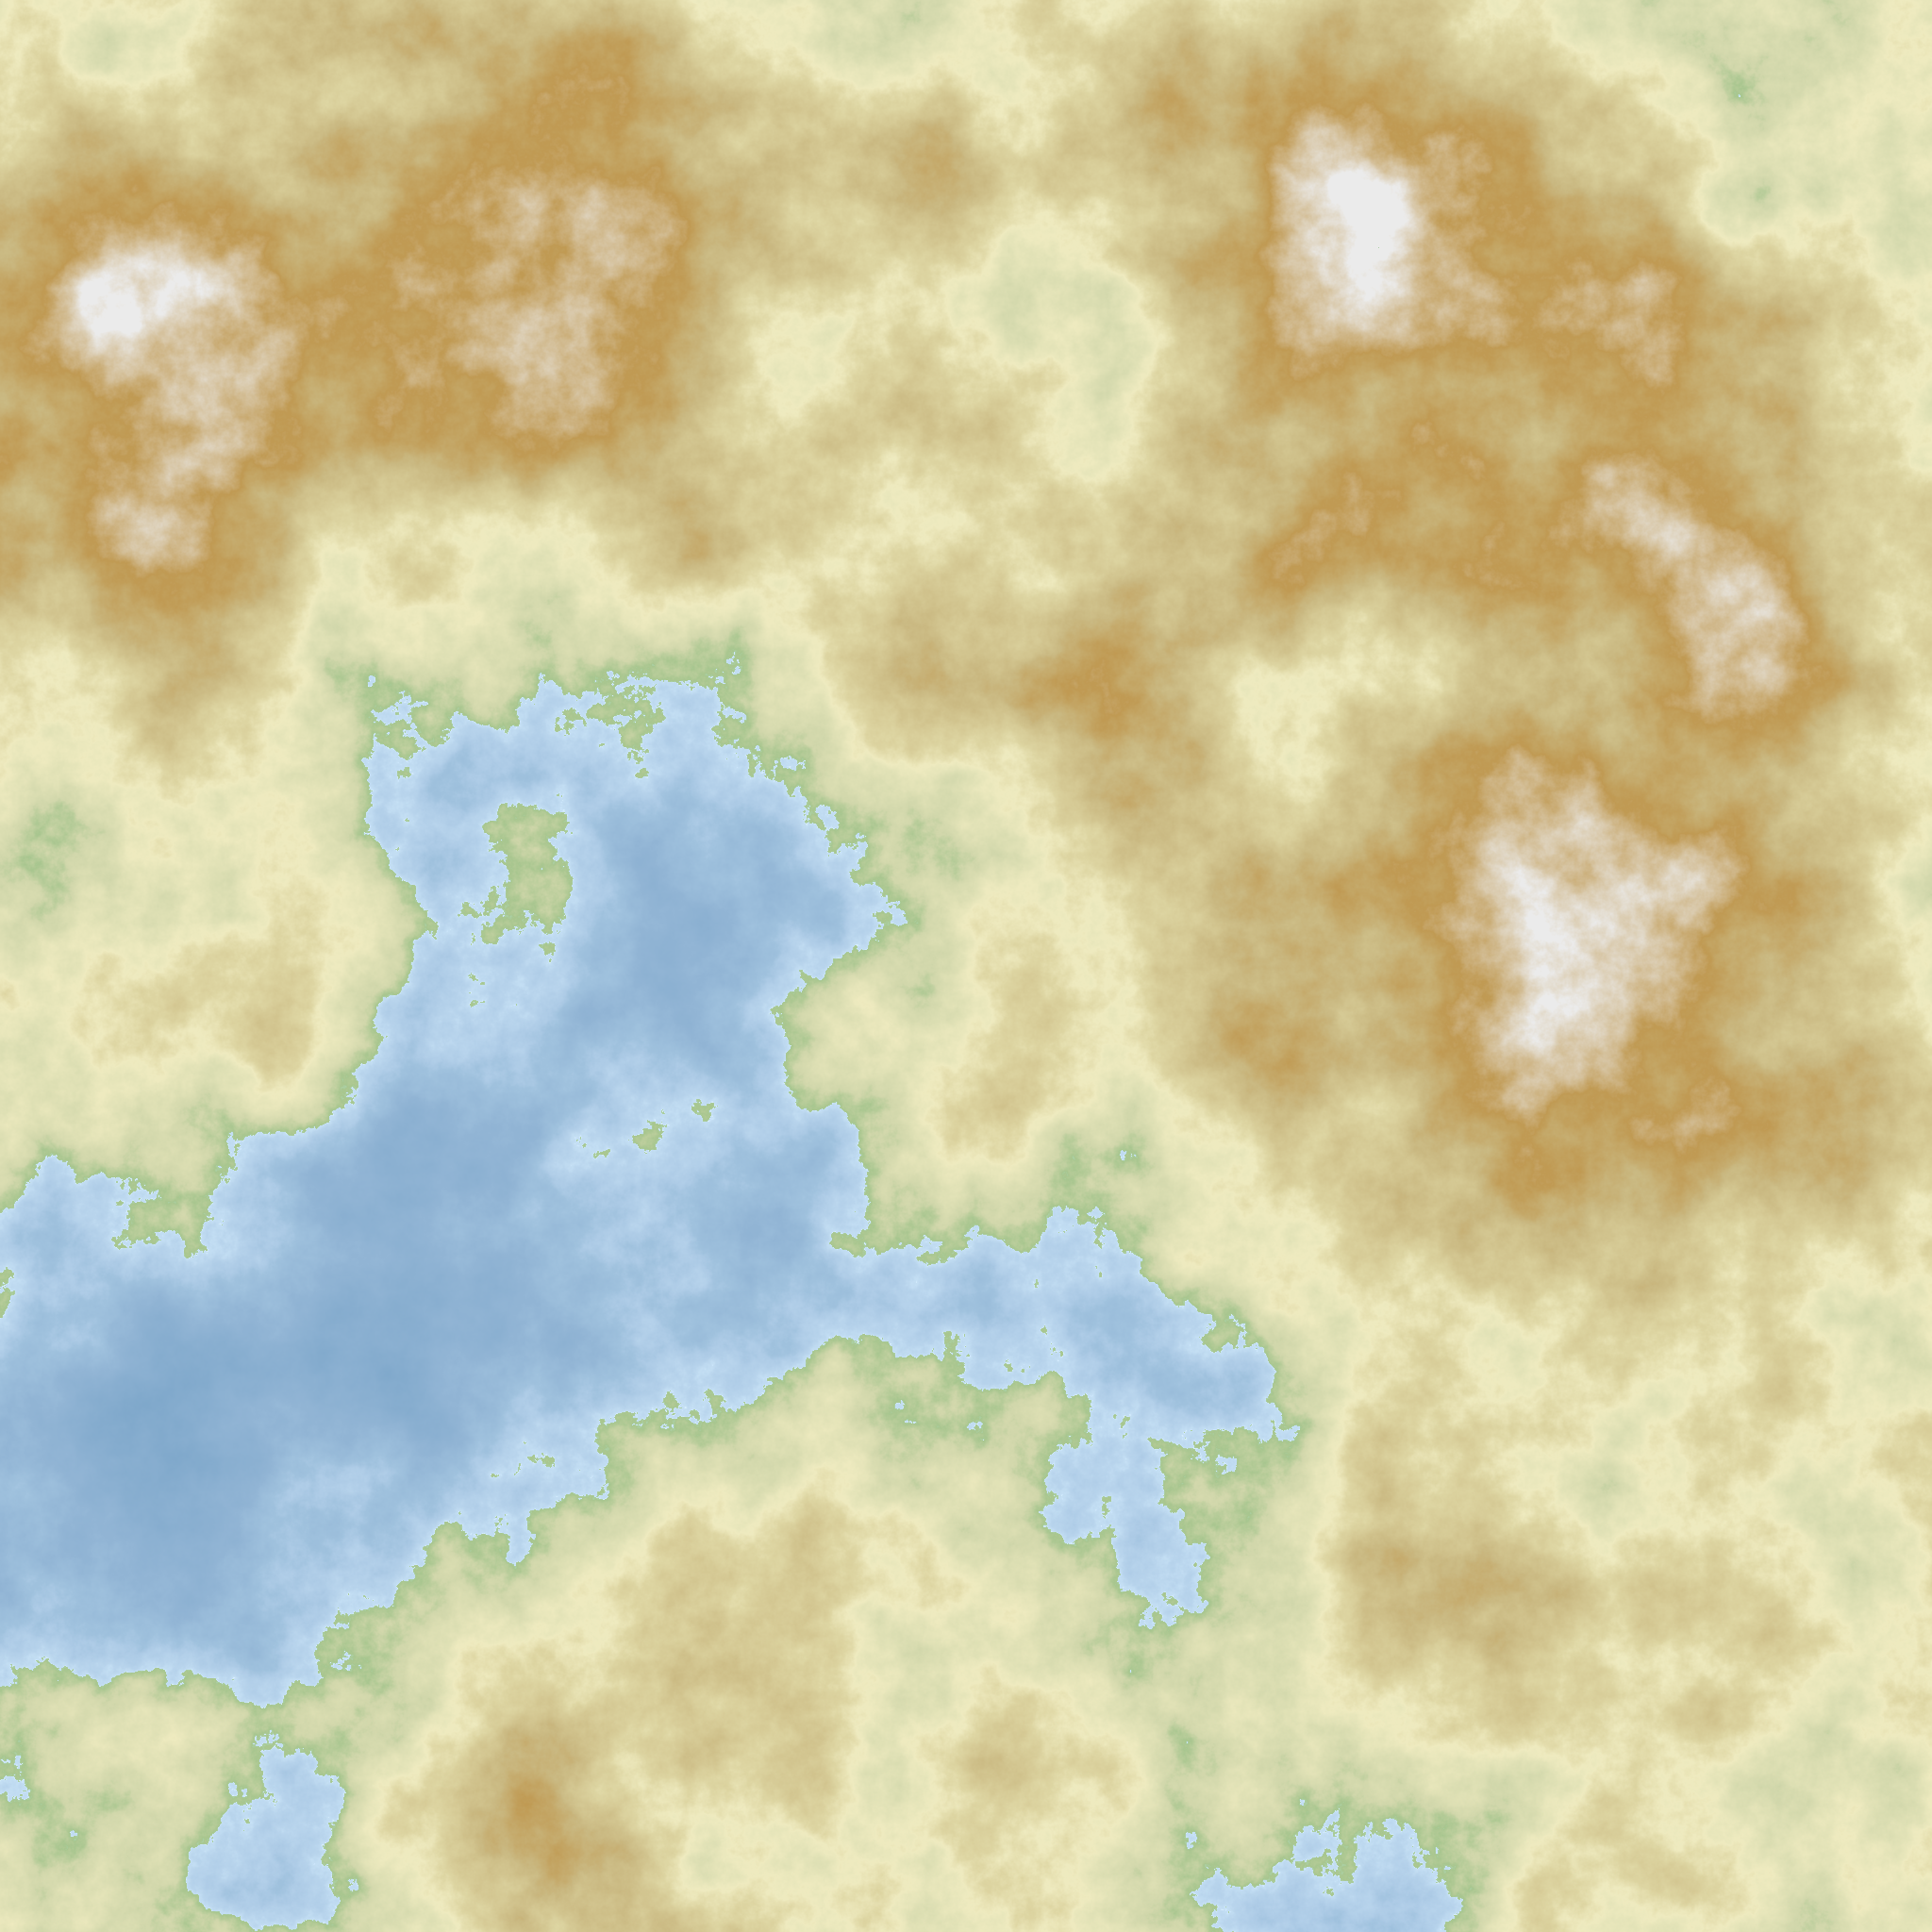
\includegraphics[width=0.4\textwidth]{data/perlin_comb_render_colored.png}
}

\ods 
Teraz bude treba zafarbený obrázok vytieňovať. Na to použijeme jednoduchý osvetľovací model
(tzv. Lambertov). Predstav si, že máš malú plôšku, ktorá má normálový vektor $\vec n$
a nejakú základnú farbu. Čím na ňu dopadá menej svetla, tým je tmavšia. Ako viem zistiť,
koľko svetla na ňu dopadá? Ak svetlo prichádza z nejakého smeru, pozriem sa na uhol
medzi zdrojom svetla a normálovým vektorom:
  
\centerline{
%\tikzset{external/force remake}
%\tdplotsetmaincoords{50}{45}
%\begin{tikzpicture}[tdplot_main_coords]
\begin{tikzpicture}[x={(1,0)}, z={(0,1)}, y={(0.5,0.5)}]
  \def\dot[#1](#2){\fill[fill=#1] (#2) circle (1.2pt) ;}
  \def\sun(#1,#2,#3){
    \begin{scope}[canvas is xz plane at y=#2]
      \begin{scope}[shift={(#1,#3)},every path/.style={fill=white,draw=orange,very thick}]
        \filldraw (0,0) circle (0.2cm);
      \def\n{20}  
        \foreach \i in {0,...,\n} {
          \pgfmathsetmacro{\tmp}{\i*360/\n}
        \draw (\tmp:0.3cm) -- (\tmp:0.4cm);
        }
    \end{scope}
    \end{scope}
  }

  \def\ax{2}\def\ay{1}\def\az{2}
  \def\sx{0}\def\sy{0}\def\sz{5}
  \def\ux{1}\def\uy{4}\def\uz{0}
  \def\vx{-1}\set{\vy}{1.0/\uy}\def\vz{0.6}

  \coordinate (Ax) at (\ax,\ay,0);
  \coordinate (h) at (0,0,\az);

  \coordinate (S) at (\sx,\sy,\sz);

  
  \normalize{\ux}{\uy}{\uz}
  \normalize{\vx}{\vy}{\vz}
  \coordinate (u) at (\ux,\uy,\uz);
  \coordinate (v) at (\vx,\vy,\vz);
  \coordinate (A) at ($(Ax)+(h)$);
  \def\s{1}
  \coordinate (P) at ($(A)-\s*(u) - \s*(v)$);
  \cross{\nx}{\ny}{\nz}{\ux}{\uy}{\uz}{\vx}{\vy}{\vz}

  \normalize{\nx}{\ny}{\nz}
  \coordinate (n) at (\nx,\ny,\nz);

  \begin{scope}[canvas is xy plane at z=0]
    \draw [gray!20, very thin] (-1,-1) grid (4,4);
  \end{scope}
  \draw[orange,thick,dotted] (\sx,\sy,0)  -- (S);
  \dot[orange](\sx,\sy,0)
 
  \coordinate (u2) at (\ux,\uy,0);
  \coordinate (v2) at (\vx,\vy,0);
  \coordinate (P2) at ($(Ax)-\s*(u2)-\s*(v2)$);


  \filldraw[fill=green!10] (P) -- ($(P)+2*\s*(u)$) --($(P)+2*\s*(u)+2*\s*(v)$) -- 
  ($(P)+2*\s*(v)$) -- cycle;
  \draw[green!50!black,thick,dotted](Ax)--($(A)+(0,0,0)$);

  \coordinate (An) at ($(A)+1.5*(n)$);
  \draw[draw=none]  pic[draw, angle radius=4ex] {angle = An--A--S};

  \draw[orange,thick,->,shorten >= 3ex] (A)--node[anchor=south west]{$\vec s$}(S);
  \draw[teal,thick,->] (A)--(An) node[anchor=west]{$\vec n$};
  \dot[green!50!black](A);
  \dot[green!50!black](Ax);
  \sun(\sx,\sy,\sz)
  \node[above=1ex] at (A) {$\alpha$};

  %\drawaxes
\end{tikzpicture}}

\ods
Kosínus tohoto uhla mi vyjadruje množstvo dopadajúceho svetla: ak plôška smeruje presne na zdroj svetla, uhol je $0$,
$\cos(0)=1$, takže farba je najsilnejšia. Ako uhol rastie, $\cos(\alpha)$ postupne klesá, až keď je uhol $90^\circ$,
tak nedopadá žiadne svetlo $\cos(90^\circ)=0$.
Ak $\vec s$ je vektor smerom k svetelnému zdroju, stačí mi znormalizovať ho
a vyrátať skalárny súčin s $\vec n$ a mám $\cos(\alpha)$, ktorý potrebujem.

\ods
Posledná otvorená otázka je, ako vyrátať normálový vektor pre nejaký pixel
vo výškovej mape. Môžem to spraviť napríklad tak, že sa pozriem na 8 okolitých pixelov. Každý z nich mi dáva trojuholník,
ktorému viem vypočítať normálový vektor pomocou vektorového súčinu. Výsledný vektor potom dostanem ako priemer 
normálových vektorov trojuholníkov:


\centerline{
%\tikzset{external/force remake}
%\tdplotsetmaincoords{50}{45}
%\begin{tikzpicture}[tdplot_main_coords]
\begin{tikzpicture}[x={(1,0)}, z={(0,1)}, y={(0.25,0.5)}, scale=3]
  \def\dot[#1](#2){\fill[fill=#1] (#2) circle (0.4pt) ;}

  \begin{scope}[canvas is xy plane at z=0]
    \draw [gray!20, very thin] (-0.5,-0.5) grid (2.5,2.5);
  \end{scope}

  \def\vaa{0.9}
  \def\vab{1.0}
  \def\vac{1.4}

  \def\vba{1.1}
  \def\vbb{1.2}
  \def\vbc{1.3}
  
  \def\vca{0.2}
  \def\vcb{0.6}
  \def\vcc{0.4}

  \def\chval#1{\if#10a\else\if#11b\else c\fi\fi}
  \def\w#1#2{\csname v\chval#1\chval#2\endcsname}
  \def\crd#1#2{#1,#2,\w{#1}{#2}}

  \coordinate (O) at (1,1,\w11);

  \coordinate (N) at (0,0,0);

  \foreach \i/\j/\ii/\jj/\f in {
    0/2/1/2/0%
    ,1/2/2/2/0%
    ,0/1/0/2/0%
    ,2/2/2/1/0%
    ,0/0/0/1/0%
    ,1/0/0/0/1%
    ,2/1/2/0/0%
    ,2/0/1/0/0%
  } {
    \draw[dotted] (\i,\j,0)--(\crd{\i}{\j}) (\ii,\jj,0) -- (\crd{\ii}{\jj});
    \filldraw[thin,gray,fill=yellow!10, opacity=0.6](\crd{\i}{\j})--(\crd{\ii}{\jj})--(\crd11)--cycle;

    \coordinate (A) at (\crd{\i}{\j});
    \coordinate (B) at (\crd{\ii}{\jj});
    \coordinate (P) at ($0.33*(A)+0.33*(B)+0.33*(O)$);
    \dot[blue](P)
    \set{\ux}{\ii-1}
    \set{\uy}{\jj-1}
    \set{\uz}{\w{\ii}{\jj}-\w11}
    \set{\vx}{\i-1}
    \set{\vy}{\j-1}
    \set{\vz}{\w{\i}{\j}-\w11}
    \cross{\nx}{\ny}{\nz}{\ux}{\uy}{\uz}{\vx}{\vy}{\vz}
    \normalize{\nx}{\ny}{\nz}
    \typeout{(\ux,\uy,\uz) x (\vx,\vy,\vz) =(nrm) (\nx,\ny,\nz)}
    \coordinate (n) at (\nx,\ny,\nz);
    \draw[blue,->](P)--($(P)+0.3*(n)$);
    \coordinate (N) at ($(N)+(n)$);
    \if\f1
      \draw[thick,red,->](O)--node[anchor=east]{$\vec u$}(A);
      \draw[thick,magenta,->](O)--node[anchor=north west, pos=0.6]{$\vec v$}(B);
    \fi
  }
  \coordinate (O) at (\crd11);
  \draw[thick,teal,->] (O) -- ($(O)+0.125*(N)$) node[above]{$\vec n$};

  \foreach \i in {0,1,2}{
    \foreach \j in {0,1,2} {
      \dot[black](\crd{\i}{\j})
    }}

    
  \draw[gray,brace=0.1ex/mirror] (0,0,0)--node[below=1.2ex]{$s$}(1,0,0);

  %\drawaxes
\end{tikzpicture}}

\ods
Naprogramovať sa to dá napríklad takto:

\ods
\begin{lstlisting}
Vec3 normala(Tabulka<double> &H, int i, int j, double s = 1) {
  Vec3 res;
  vector<Vec> dir{{0, 1},   {1, 1},  {1, 0},  {1, -1}, {0, -1},
                  {-1, -1}, {-1, 0}, {-1, 1}, {0, 1}};
  for (int t = 0; t < dir.size() - 1; t++) {
    int i0 = i + dir[t].x,     j0 = j + dir[t].y, 
        i1 = i + dir[t + 1].x, j1 = j + dir[t + 1].y;
    res +=
        -1.0 *
        (
         (Vec3{s * dir[t].x, s * dir[t].y, H(i0, j0)} 
          - Vec3{0, 0, H(i, j)}) 
          ^ // vektorovy sucin
         (Vec3{s * dir[t + 1].x, s * dir[t + 1].y, H(i1, j1)} -
          Vec3{0, 0, H(i, j)})
        );
  }
  return res.normalize();
}
\end{lstlisting}

\ods
Táto funkcia dostane ako parameter tabuľku {\tt H} a pozíciu pixela {\tt i,j}.
Navyše dostanem parameter {\tt s}, ktorý hovorí, ako ďaleko sú od seba jednotlivé pixely
(t.j. výškovú mapu si predstavujem ako sieť s krokom {\tt s}).

\ods
Pre obrázok s rozmermi $2048\times2048$ som si nastavil smer svetla na 
\prg!Vec3 light{-1, 1, 12};! a \prg!double s=0.004;! a 
z výškovej mapy {\tt H} som si vyrátal tabuľku \prg!Tabulka<double> N!
takto:

\begin{lstlisting}
light.normalize();
for (int i = 0; i < H.m; i++)
  for (int j = 0; j < H.n; j++)
    if (H(i, j) <= wl)
      N(i, j) = 1;
    else
      N(i, j) = light * normala(H, i, j, s);
\end{lstlisting}

\ods
Výsledok je na obrázku vľavo. Obrázok vpravo vznikol tak, že som každú farbu pixela na ofarbenej mape
prenásobil koeficientom \prg!0.6 + 0.4 * max(0.0, N(i, j));!

\ods
\centerline{
  
\includegraphics[width=0.4\textwidth]{data/perlin_comb_render_normal.png}
  \hskip 1cm
  \includegraphics[width=0.4\textwidth]{data/perlin_comb_render_rendered.png}
}

\ods
Toto už vyzerá ako mapa terénu, aj keď zrovna ostrov to nie je. To sa dá ale ľahko napraviť pri generovaní
výškovej mapy: okrem Perlinovho šumu sa navyše každý bod posunie dole úmerne jeho vzdialenosti od stredu 
obrázka. Okraje klesnú a v strede ostane ostrov. S trochou hrania sa s parametrami som dospel k takémuto
výsledku:

\ods
\centerline{
  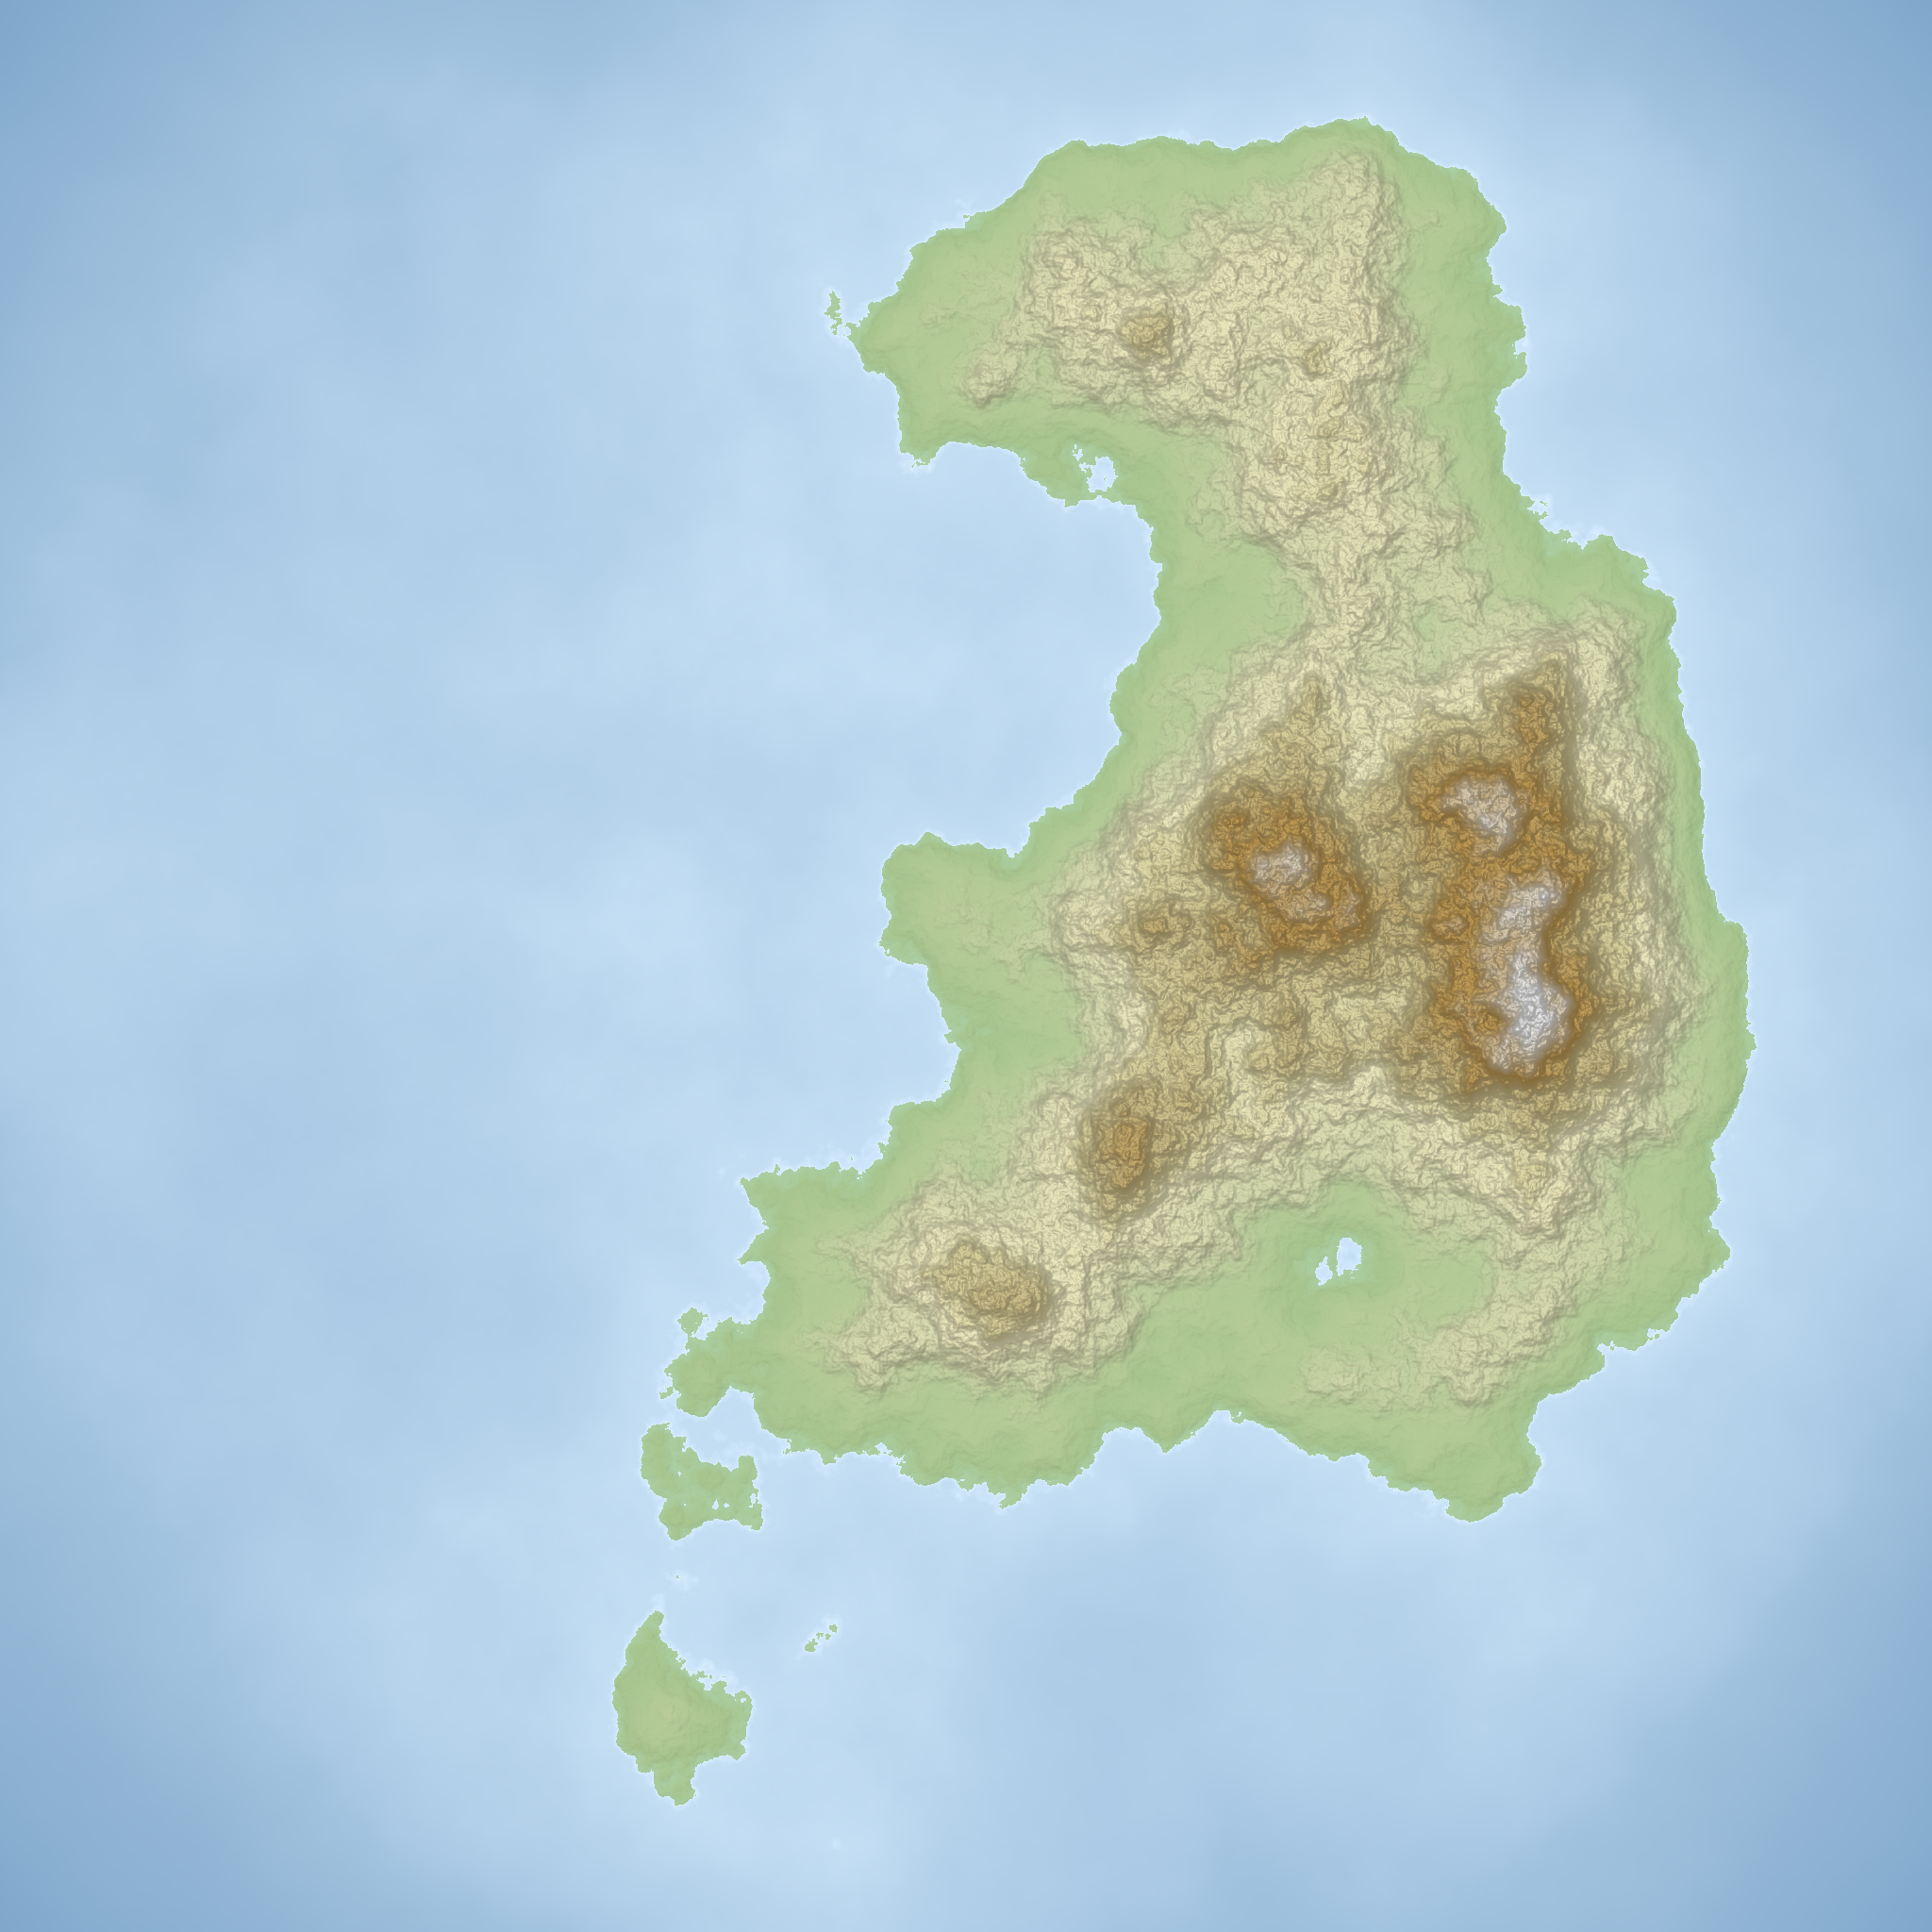
\includegraphics[width=0.8\textwidth]{data/86_rendered_dry.png}
}

\ods
Úplne posledná vec, ktorá tomu chýba, sú doliny riek a fjordy. Rozhodol som sa preto spraviť jednoduchú
fyzikálnu simuláciu vodnej erózie. Urobiť realistickú virtuálnu eróziu je téma sama osebe, ale 
v \link%
{https://www.firespark.de/resources/downloads/implementation\%20of\%20a\%20methode\%20for\%20hydraulic\%20erosion.pdf}%
{bakalárskej práci Hansa Beyera}
je veľmi zjednodušený a ľahko naprogramovateľný prístup, ktorý si tu môžeme vyskúšať.
Hlavná idea je, že na povrch našej výškovej mapy budeme púšťať kvapky\footnote{
  Vzhlľadom na mierku, ktorú máme, to bude skôr ako futbalový štadión plný vody, ale
  volajme to kvapka.}. Kvapka má nejaký objem vody a v nej je rozpusteny nejaky objem 
bahna. Ak je bahna málo a kvapka ide rýchlo, vymyje kúsok z povrchu: výšková mapa sa trochu 
zníží a v kvapke bude viac bahna. Naopak, ak je bahna veľa a kvapka ide pomaly, bahno sa bude
usadzovať: v kvapke ho ostane menej a povrch sa trochu zvýši.


\centerline{
\tikzset{external/force remake}
%\tdplotsetmaincoords{50}{45}
%\begin{tikzpicture}[tdplot_main_coords]
\begin{tikzpicture}[x={(1,0)}, z={(0,1)}, y={(0.5,0.5)}]
%\begin{tikzpicture}[x={(1,0)}, z={(0,0)}, y={(0,1)}]
  \def\dot[#1](#2){\fill[fill=#1] (#2) circle (1.2pt) ;}

  \def\rotplane[#1][#2][#3]{ %zxz
    \def\h{1}
    \def\d{1}
    \set{\ax}{-0.5*\d}\set{\ay}{-0.5*\d}\set{\az}{0}
    \set{\bx}{0.5*\d}\set{\by}{-0.5*\d}\set{\bz}{0}
    \set{\cx}{0.5*\d}\set{\cy}{0.5*\d}\set{\cz}{0}
    \set{\dx}{-0.5*\d}\set{\dy}{.5*\d}\set{\dz}{0}
    \set{\nx}{0}\set{\ny}{0}\set{\nz}{1}

    \rotz[#1]{\ax}{\ay}{\az}
    \rotz[#1]{\bx}{\by}{\bz}
    \rotz[#1]{\cx}{\cy}{\cz}
    \rotz[#1]{\dx}{\dy}{\dz}
    \rotz[#1]{\nx}{\ny}{\nz}

    \rotx[#2]{\ax}{\ay}{\az}
    \rotx[#2]{\bx}{\by}{\bz}
    \rotx[#2]{\cx}{\cy}{\cz}
    \rotx[#2]{\dx}{\dy}{\dz}
    \rotx[#2]{\nx}{\ny}{\nz}

    \rotz[#3]{\ax}{\ay}{\az}
    \rotz[#3]{\bx}{\by}{\bz}
    \rotz[#3]{\cx}{\cy}{\cz}
    \rotz[#3]{\dx}{\dy}{\dz}
    \rotz[#3]{\nx}{\ny}{\nz}

    \begin{scope}[shift={(0,0,\h)}]
    \draw (\ax,\ay,\az) -- (\bx,\by,\bz) -- (\cx,\cy,\cz) -- (\dx,\dy,\dz) -- cycle;
    \draw[->] (0,0,0) -- (\nx,\ny,\nz);
    \dot[black](0,0,0);
    \end{scope}

    \draw[dashed] (0,0,0) -- (0,0,\h);
    \draw[green] (0,0,0) -- (\nx,\ny,0);

  }

  \begin{scope}[canvas is xy plane at z=0]
    \draw [gray!20, very thin] (-1.5,-1.5) grid (1.5,1.5);
  \end{scope}

  \rotplane[0][45][50]
  \begin{scope}[shift={(2,0)}]
    \rotplane[0][0][0]
  \end{scope}


  %\drawaxes
\end{tikzpicture}}






\centerline{
\tikzset{external/force remake}
\begin{tikzpicture}[x={(1,0)}, z={(0,0.7)}, y={(0.25,0.5)}, scale=3.5]
%\begin{tikzpicture}[x={(1,0)}, z={(0,0)}, y={(0,1)}, scale=3.5]
  \def\dot[#1](#2){\fill[fill=#1] (#2) circle (0.4pt) ;}

  \begin{scope}[canvas is xy plane at z=0]
    \draw [gray!20, very thin] (-0.2,-0.2) grid (1.2,1.2);
  \end{scope}

  \def\vs{0.5}
  \def\newv(#1)#2#3#4{
    \def\tmpx{#2}
    \def\tmpy{#3}
    \def\tmpz{#4}
    \normalize{\tmpx}{\tmpy}{\tmpz}
    \coordinate (#1) at (\vs*\tmpx,\vs*\tmpy,\vs*\tmpz);
    \coordinate (#1!0) at (\vs*\tmpx,\vs*\tmpy,0);
  }
  \def\chval#1{\if#10a\else\if#11b\else\if#12c\else d\fi\fi\fi}
  \def\w#1#2{\csname v\chval#1\chval#2\endcsname}
  \def\crd#1#2{#1,#2,\w{#1}{#2}}

  \def\vaa{1.0} \newv(n00){-0.2}{-0.3}{1}
  \def\vab{1.3} \newv(n01){-0.2}{-0.7}{1.5}

  \def\vba{0.8} \newv(n10){-0.2}{-0.3}{1}
  \def\vbb{1.5} \newv(n11){-0.2}{-0.7}{1} 
  
  \foreach \i in {0,1}{
    \foreach \j in {0,1} {
      \coordinate (A\i\j) at (\crd{\i}{\j});
      \coordinate (A\i\j!0) at (\i,\j,0);
    }}


  \def\px{0.5} \def\py{0.7}


  \coordinate (P!0) at (\px,\py,0);
  \coordinate (P0!0) at (\px,0,0);
  \coordinate (P1!0) at (\px,1,0);

  \coordinate (P0) at ($(A00)!\px!(A10)$);
  \coordinate (P1) at ($(A01)!\px!(A11)$);
  \coordinate (P) at ($(P0)!\py!(P1)$);

  \foreach \a in {0,1}{
  \coordinate (nP\a) at ($(n0\a)!\px!(n1\a)$);
  \coordinate (nP\a!0) at ($(n0\a!0)!\px!(n1\a!0)$);
  }
  \coordinate (nP) at ($(nP0)!\py!(nP1)$);
  \coordinate (nP!0) at ($(nP0!0)!\py!(nP1!0)$);



  \foreach \a in {0,1}{
  \draw[green,->] (P\a)--($(P\a)+(nP\a)$);
  \draw[green,->](P\a!0)--($(P\a!0)+(nP\a!0)$);
  }
  \draw[green,->] (P)--($(P)+(nP)$);
  \draw[green,->](P!0)--($(P!0)+(nP!0)$);

  %\draw let \p1=(nP0!0),\p2=(n00!0),\p3=(n10!0) in (2,0) node{\x1,\y1 :: \x2,\y2 :: \x3,\y3};
  

  \draw (A00) -- (A10) -- (A11) -- (A01) -- cycle;
  \foreach \X in {P,P0,P1}{
  \dot[red](\X!0)
  \dot[magenta](\X)
}



  \foreach \i in {0,1}{
    \foreach \j in {0,1} {
      \draw[teal,->] (A\i\j) -- ($(A\i\j)+(n\i\j)$);
      \draw[cyan,->] (A\i\j!0) -- ($(A\i\j!0)+(n\i\j!0)$);

      \dot[black](A\i\j)
      \draw[dashed,gray,thin] (A\i\j!0) -- (A\i\j);
    }}


  %\drawaxes
\end{tikzpicture}}




\ods
\centerline{
  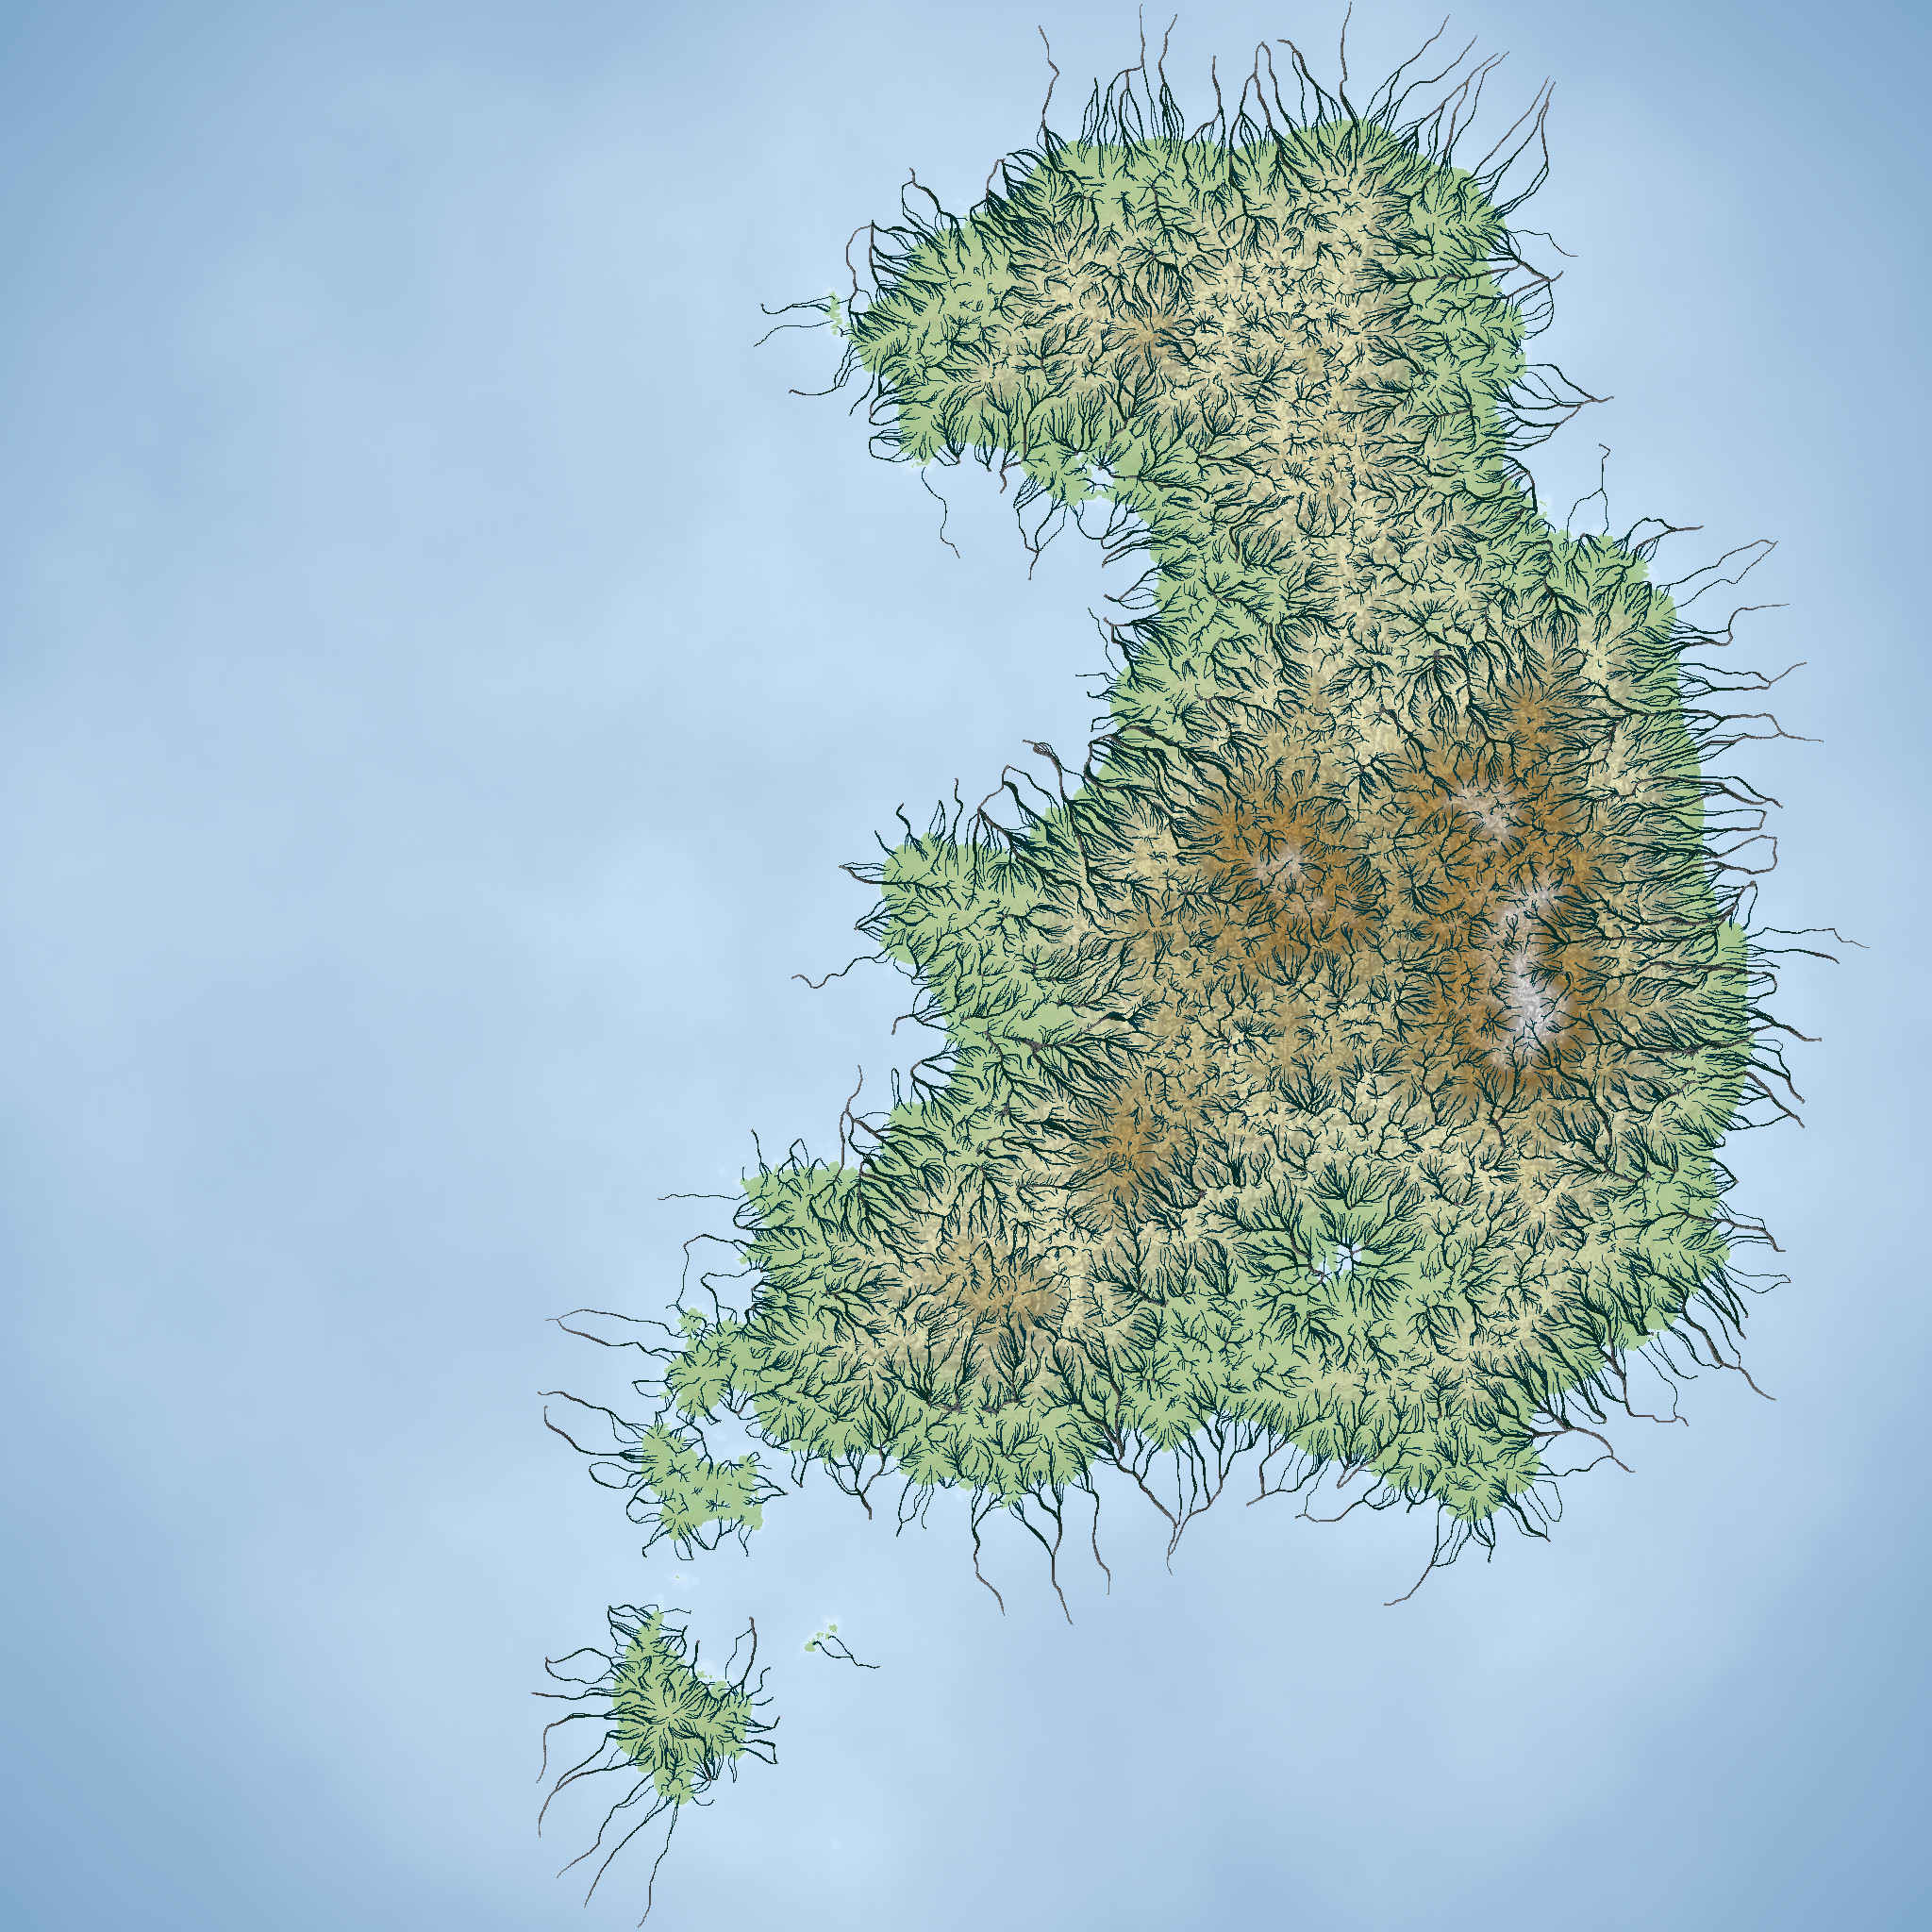
\includegraphics[width=0.4\textwidth]{data/86_rendered_droplets.png}
  \hskip 1cm
  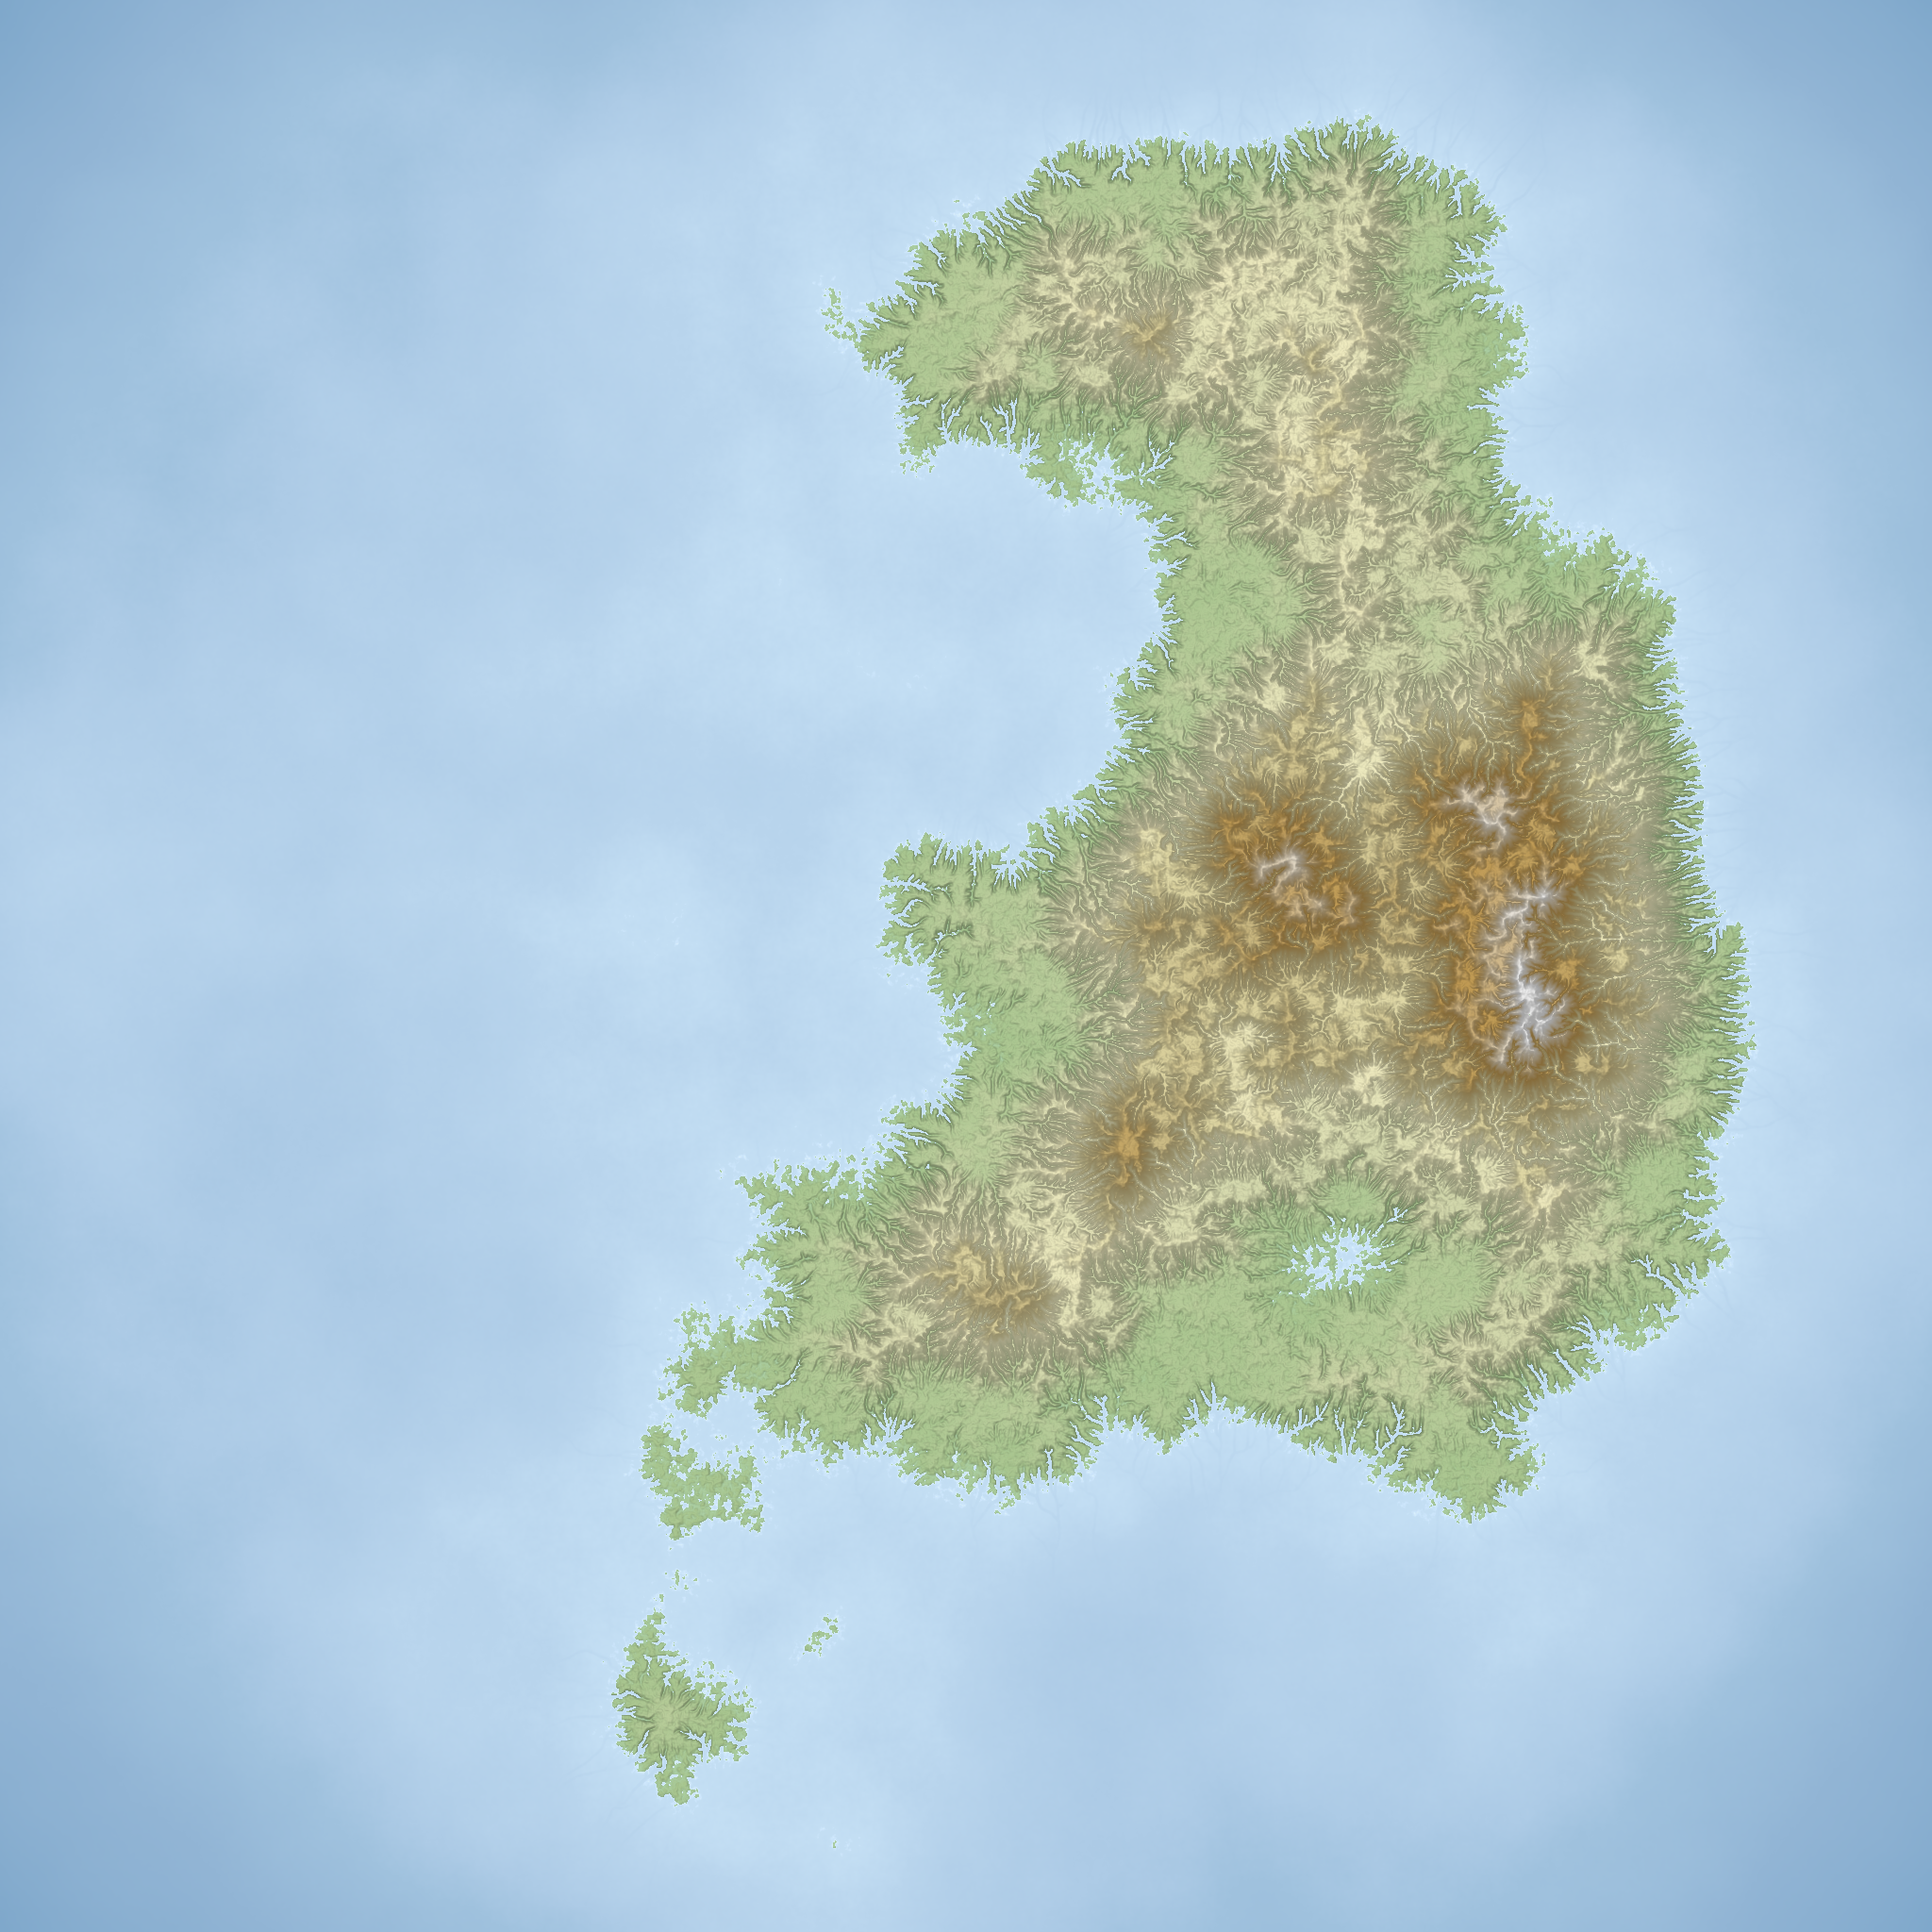
\includegraphics[width=0.4\textwidth]{data/86_rendered.png}
}

\fi

% pridat k funkciam - vypisat zarovnanu tabulku n x n
%  hasovanie

% projekt breakthrough (rozdelit veci do suborov, dedenie)
% grafika SDL (GUI - sofistikovanejsei dedenie, virtualne metody)
% thready



% NN

\end{document}
%%%%%%%%%%%%%%%%%%%%%%%%%%%%%%%%%%%%%%%%%%%%%%%%%%%%%%%%%%%%%%%%%%%%%%%%%%%%%%
\IGNORE{
\ods
Predstav si, že budem hádzať dvoma kockami a budem sa pozerať na súčet čísel
na oboch. Aké je priemerné číslo, ktoré mi budem dostávať?
Lákalo by to k takejto úvahe: môže mi padnúť $11$ rôznych súčtov: od $2$ po $12$.
Priemer je preto $(2+3+\cdots+12)/11=7$. Lenže napr. súčet $2$ mi môže padnúť iba jedným 
spôsobom, t.j. s pravdepodobnosťou $\frac{1}{36}$, ale napr. 
súčet $7$ šiestimi, t.j. s pravdepodobnosťou $\frac{6}{36}=\frac{1}{6}$. Preto 
súčet $7$ sa bude vyskytovať oveľa častejšie.

\ods
V matematike sa {\em náhodná premenná} volá niečo, čo viem vyrátať z náhodného javu. Napr.
ak hodím dve kocky, tak viem vyrátať súčet bodiek -- súčet bodiek je preto náhodná premenná.
{\em Stredná (očakávaná) hodnota} náhodnej premennej je priemerná hodnota výsledku, ktorý 
budem dostávať. Ak 
}

\IGNORE{
\ods
Ak mám vektor $\vec v$ so súradnicami $[x,y]$

\ods
\centerline{
  \begin{tikzpicture}[scale=4]
  \def\an{40}
  \def\ra{0.4ex}
    \draw[thin,dotted,step=0.5](-0.5,-0.5) grid (1,1);
    \draw(1.1,0) -- (0,0) node[anchor=north east]{$O=[0,0]$} -- (\an:1.1);

    \draw[red](1ex,0) arc (0:\an:1ex) node[midway,anchor=west]{$\alpha$};
    \draw[thin,gray](-35:1) arc (-35:125:1);

    \draw[-{>[length=3ex,width=1ex]},thin,gray] (0,0) -- (110:1) ;

    \coordinate (B) at (\an:1);
    \draw[red,-{>[length=3ex,width=1ex]}](0,0)--(B) node[midway,anchor=south east]
      {$\nrm{\vec v}$};
    \node[right=3mm of B]  {$B=[x,y]$};

    \draw[blue] (B) -- (B|-0,0) coordinate (A) node[midway, anchor=west] {$y = \sin(\alpha)$};
    \node[anchor=north west] at (A) {$A$};
    
    \draw (A)+(0,\ra) arc (90:180:\ra);
    \filldraw (A)+(-\ra/3,\ra/3) circle (.1pt);

    \def\g{rgb:green,5;yellow,4;blue,2;black,3}
    \draw[thick,draw=\g](0,0)--(A) 
    node[midway,anchor=north]{\textcolor{\g}{$x = \cos(\alpha)$}};
\end{tikzpicture}}
}

